\documentclass[12pt,twoside,a4paper]{article} 
\usepackage{fullpage}
\usepackage{graphicx}
\usepackage{enumerate}
\usepackage{float}
\usepackage{url} % Better display of ~ tilde
\usepackage{amsmath}
\usepackage{nccmath}
\usepackage{amssymb}
\usepackage{arcs}
\usepackage[polish,english]{babel} 
\usepackage{mathabx}
\usepackage[plmath,MeX]{polski} 
\usepackage[utf8]{inputenc}
\usepackage[font=footnotesize,format=plain,labelfont=bf,up,textfont=it,up]{caption}
\usepackage{mathtools}
\usepackage{listings}
\lstset{basicstyle=\tiny, language=Matlab}


\def\emptyline{\vspace{12pt}}
\pagenumbering{arabic}
\graphicspath{{./../}} % A path to the graphics directory
\numberwithin{equation}{subsection}
\numberwithin{figure}{subsection}
\selectlanguage{english} % We choose the auto-generated texts' language to be English
\addtolength{\voffset}{-1.0cm}
\inputencoding{utf8}
% \linespread{1.7} % bigger interline

\pagestyle{plain}
\title{Numerical evaluation of the Hilbert transform in~nonlinear optics}
 \author{Krzysztof Parjaszewski}
 \date{}
\def\Xint#1{\mathchoice
{\XXint\displaystyle\textstyle{#1}}%
{\XXint\textstyle\scriptstyle{#1}}%
{\XXint\scriptstyle\scriptscriptstyle{#1}}%
{\XXint\scriptscriptstyle\scriptscriptstyle{#1}}%
\!\int}
\def\XXint#1#2#3{{\setbox0=\hbox{$#1{#2#3}{\int}$ }\vcenter{\hbox{$#2#3$ }}\kern-.6\wd0}}
\def\ddashint{\Xint=} 
\def\dashint{\Xint-}
\newcommand{\ket}[1]{|#1\rangle}


\begin{document}

% \setlength{\parindent}{1\zw}
% \setlength{\baselineskip}{1.7\zw}

\maketitle


\begin{figure}[h]
  \begin{center}
    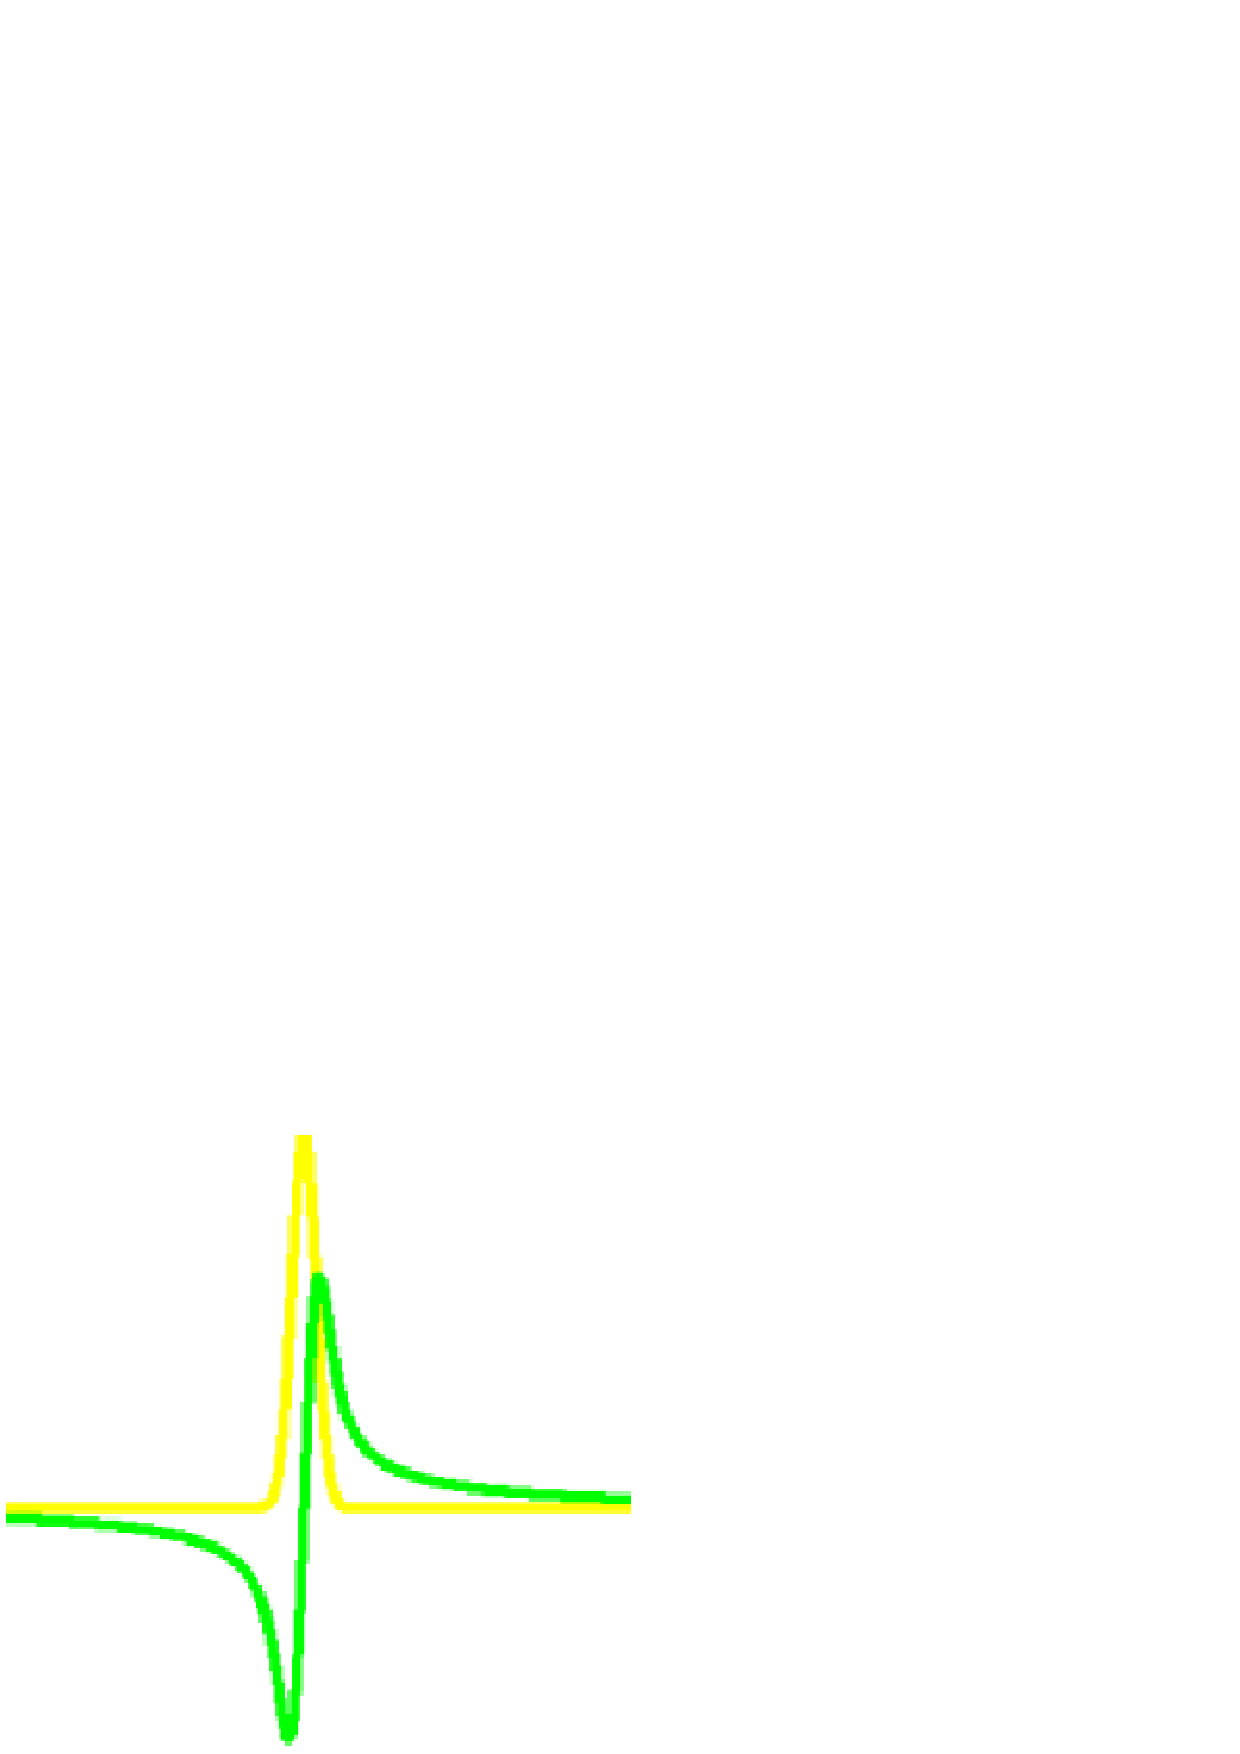
\includegraphics{img/title.png}
  \end{center}
\end{figure}


\section*{} \label{chap:preamble} 
\subsection*{Dedication} \label{chap:pre_dedication}


To my Family.


\section*{Abstract} \label{chap:abstract}

The motivation for this work comes from the real problem stated by physicists and chemists employing theoretical models to
describe the interaction between light and matter due to the low-level and intense light irradiation. We are interested in the light
behaviour both in the frequency and time domains. In the frequency domain the behaviour of light can be described with the Hilbert
transform, but to build a valid models - we need to handle two important problems. The first problem concerns the numerical evaluation
of the Hilbert Transform, which is defined with the singular and improper integral. The second problem concerns the question stated by
physicists: How to properly use these mathematical tools in a typical experiment and in the construction of a model useful in optical
research? We present comparison of several implementations of the numerical calculations of the Hilbert transform:

\begin{itemize} \label{used_methods}
 \item Numerical trapezoidal rule mixed with the Simpson's rule and the
cubic interpolation,
 \item Newton-Cotes quadrature of the sixth degree,
 \item Clenshaw-Curtis quadrature,
 \item Hilbert transform based on fast Hartley transforms,
 \item a method based on approximation with the orthonormal Hermite polynomials and Hermite functions,
 \item a method based on approximation with the Fourier series.
\end{itemize}

We also test two out-of-the-box MATLAB-implemented routines \texttt{quadgk} and \texttt{hil\-bert} - based on the fast Fourier
transform. The given physical models for both linear and nonlinear optics are analyzed and validated. We formulate hints for good
practises for scientists interested in the subject of optical experiments. Finally, we make conclusions about the numerical stability, advantages
and disadvantages of the developed implementations in further research on nonlinear optics.

\emptyline

\subsection*{Keywords} \label{chap:abstract_keywords}
numerical integration, Cauchy principal value integral, Hilbert transform, nonlinear optics, Kramers-Kronig relations, optical dispersion
relations

\subsection*{Promoters} \label{chap:abstract_promotors}

\subsubsection*{Nonlinear optics}

\textbf{Professor Marek Samoć} \\
Institute of Physical and Theoretical Chemistry \\
Wrocław University of Technology, PL-50-370 Wrocław \\
Wybrzeże Wyspiańskiego 27, Poland \\
+48-71-320-4466 | E-mail: Marek.Samoc@pwr.wroc.pl

\subsubsection*{Numerical analysis}

\textbf{Paweł Keller PhD} \\
Numerical Analysis Research Group, Institute of Computer Science \\
University of Wrocław, PL-50-383 Wrocław \\
Joliot-Curie 15, Poland \\
+48-71-375-7813 | E-mail: Pawel.Keller@ii.uni.wroc.pl


\subsection*{Reviewer}  \label{chap:abstract_reviewer}

\textbf{Professor Stanisław Lewanowicz} \\
Numerical Analysis Research Group, Institute of Computer Science \\
University of Wrocław, PL-50-383 Wrocław \\
Joliot-Curie 15, Poland \\
+48-71-375-7813 | E-mail: Stanislaw.Lewanowicz@ii.uni.wroc.pl

\subsection*{Author}  \label{chap:abstract_author}

\textbf{Krzysztof Parjaszewski} \\
Institute of Computer Science \\
University of Wrocław, PL-50-383 Wrocław \\
Joliot-Curie 15, Poland \\
+48-660-070-043 | E-mail: krzysztof.parjaszewski@gmail.com

\section{Practical motivations} \label{chap:practical_motivations}
Physics and chemistry are two scientific domains strictly connected with mathematics and the numerical analysis. Playing with the
experimental results and theoretical models scientists need the tools allowing them to validate or falsify their hypothesis, conclusions and
observations~(Figure \ref{fig:practical_nlo}).


\begin{figure} 
 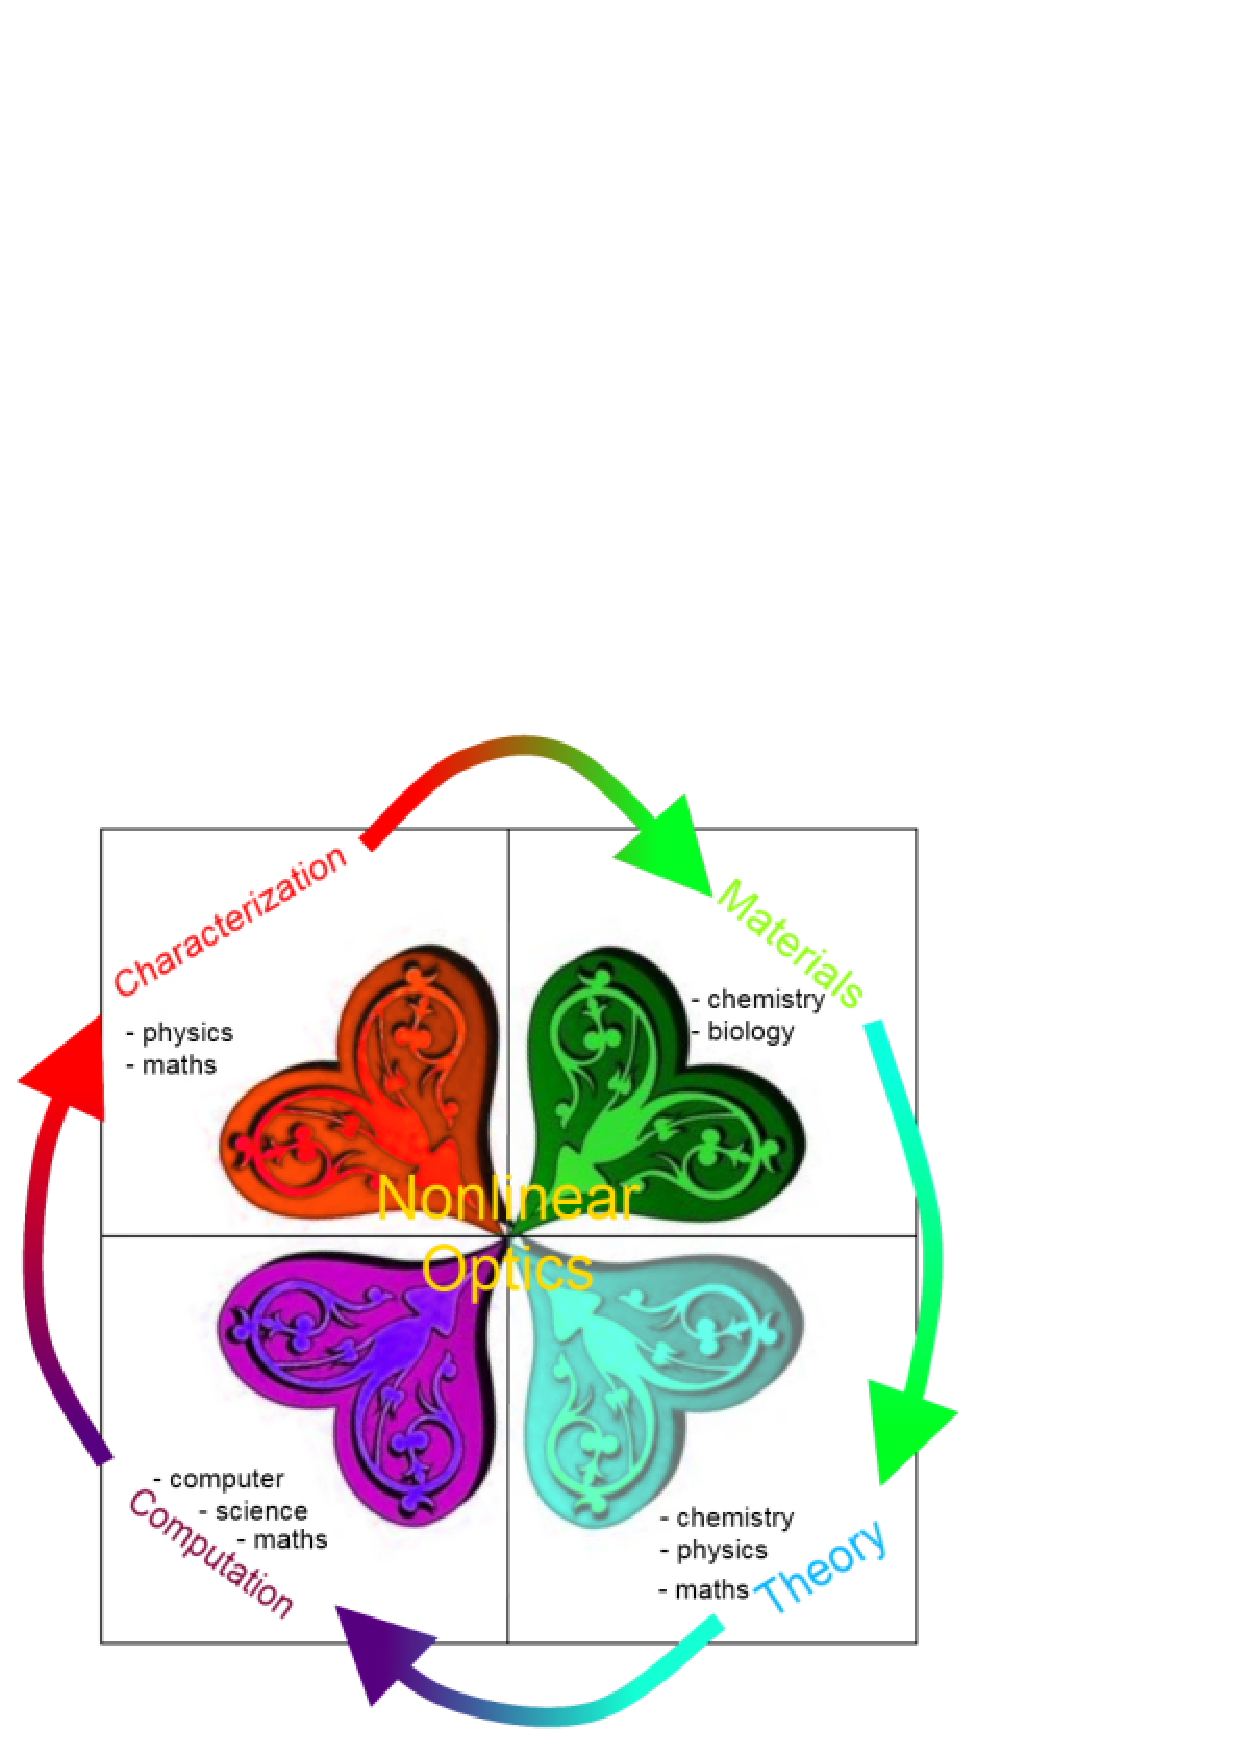
\includegraphics{img/nlo.png}
 \caption{Nonlinear optics derives from many fundamental disciplines: biology, chemistry, maths, physics and computer science.
 \label{fig:practical_nlo}}
\end{figure}


The first motivation for this thesis was the problem stated by physicians and chemists about the complex physical quantity called the
optical susceptibility denoted with $\chi$:

\begin{equation} \label{eq:pra_susceptibility}
	\chi = \Re (\chi) + \Im (\chi) . 
\end{equation}

The real part of the optical susceptibility is related with an optical phenomena - the refraction of light.
The imaginary part of the susceptibility is connected with the absorption of light. In many models these two physical quantities are connected
to each other with the modified Hilbert transform called the Kramers-Kronig relations:


\begin{equation} \label{eq:pra_hilbert_connection} 
	 \Re (\chi)  \overset{\mathcal{H}}{\rightleftharpoons} \Im (\chi) .
\end{equation}

The scientists require both mathematical and numerical tools to better understand the properties of the light beam interaction with matter. 

In this thesis we have prepared and discussed several tools that evaluates the Hilbert transform, which together with the proper physical
models, help to find a connection between the real and imaginary part of the optical susceptibility.   

The subject of this thesis is not only an academic exercise - in the last twenty years the global interest in photonics, and
especially application of light in modern devices for information transfer, storage and processing - including the construction of super-fast
all-optical computers - is steadily increasing. Recent years have seen much focus on the science and technology of photonics on
nano scale. 

This thesis consists of three important fragments. In the first fragment we have prepared the introduction into the mathematical calculations
(Chapter \ref{chap:mathematical_calculations}) and the overview of the theoretical physical models we will be using to check the
prepared numerical methods (Chapter \ref{chap:physical_models}). In the second fragment of this thesis we have prepared the short description of
each Hilbert transform evaluating methods (Chapters \ref{chap:htran} - \ref{chap:matlab}). In the last fragment we have compared the obtained
results (Chapter \ref{chap:comparison}) and drew the final conclusions (Chapter \ref{chap:conclusion}). You can also find the attached
source code in the document appendices.

The second motivation for this Thesis was to prepare a set of numerical tools for the advanced optical experiment called the
Z-Scan experiment, which has been described in the Appendix B.

\section{Mathematical calculations} \label{chap:mathematical_calculations}

\subsection{Hilbert transform - introduction}  \label{chap:mathematical_hilbert}

To define the Hilbert transform we will need to firstly define the convolution operator~$\convolution$. In the area of functional analysis
in mathematics the convolution is defined as the integral of a product of two functions, but one of them is shifted and
reversed~\cite{bracewell_fourier}:

\begin{equation} \label{eh:mth_convolution}
	(f \convolution g)(x) \stackrel{\mathrm{def}}{=}\  \int_{-\infty }^{\infty } f(\omega) \, g(x - \omega) d\omega .
\end{equation}
 
The result of the convolution of two functions $f$ and $g$ is a third function $h$ than can be described as the area overlap. The example
has been presented on Figure~(\ref{fig:mathematical_convolution}).

\begin{figure} 
	\begin{center}
		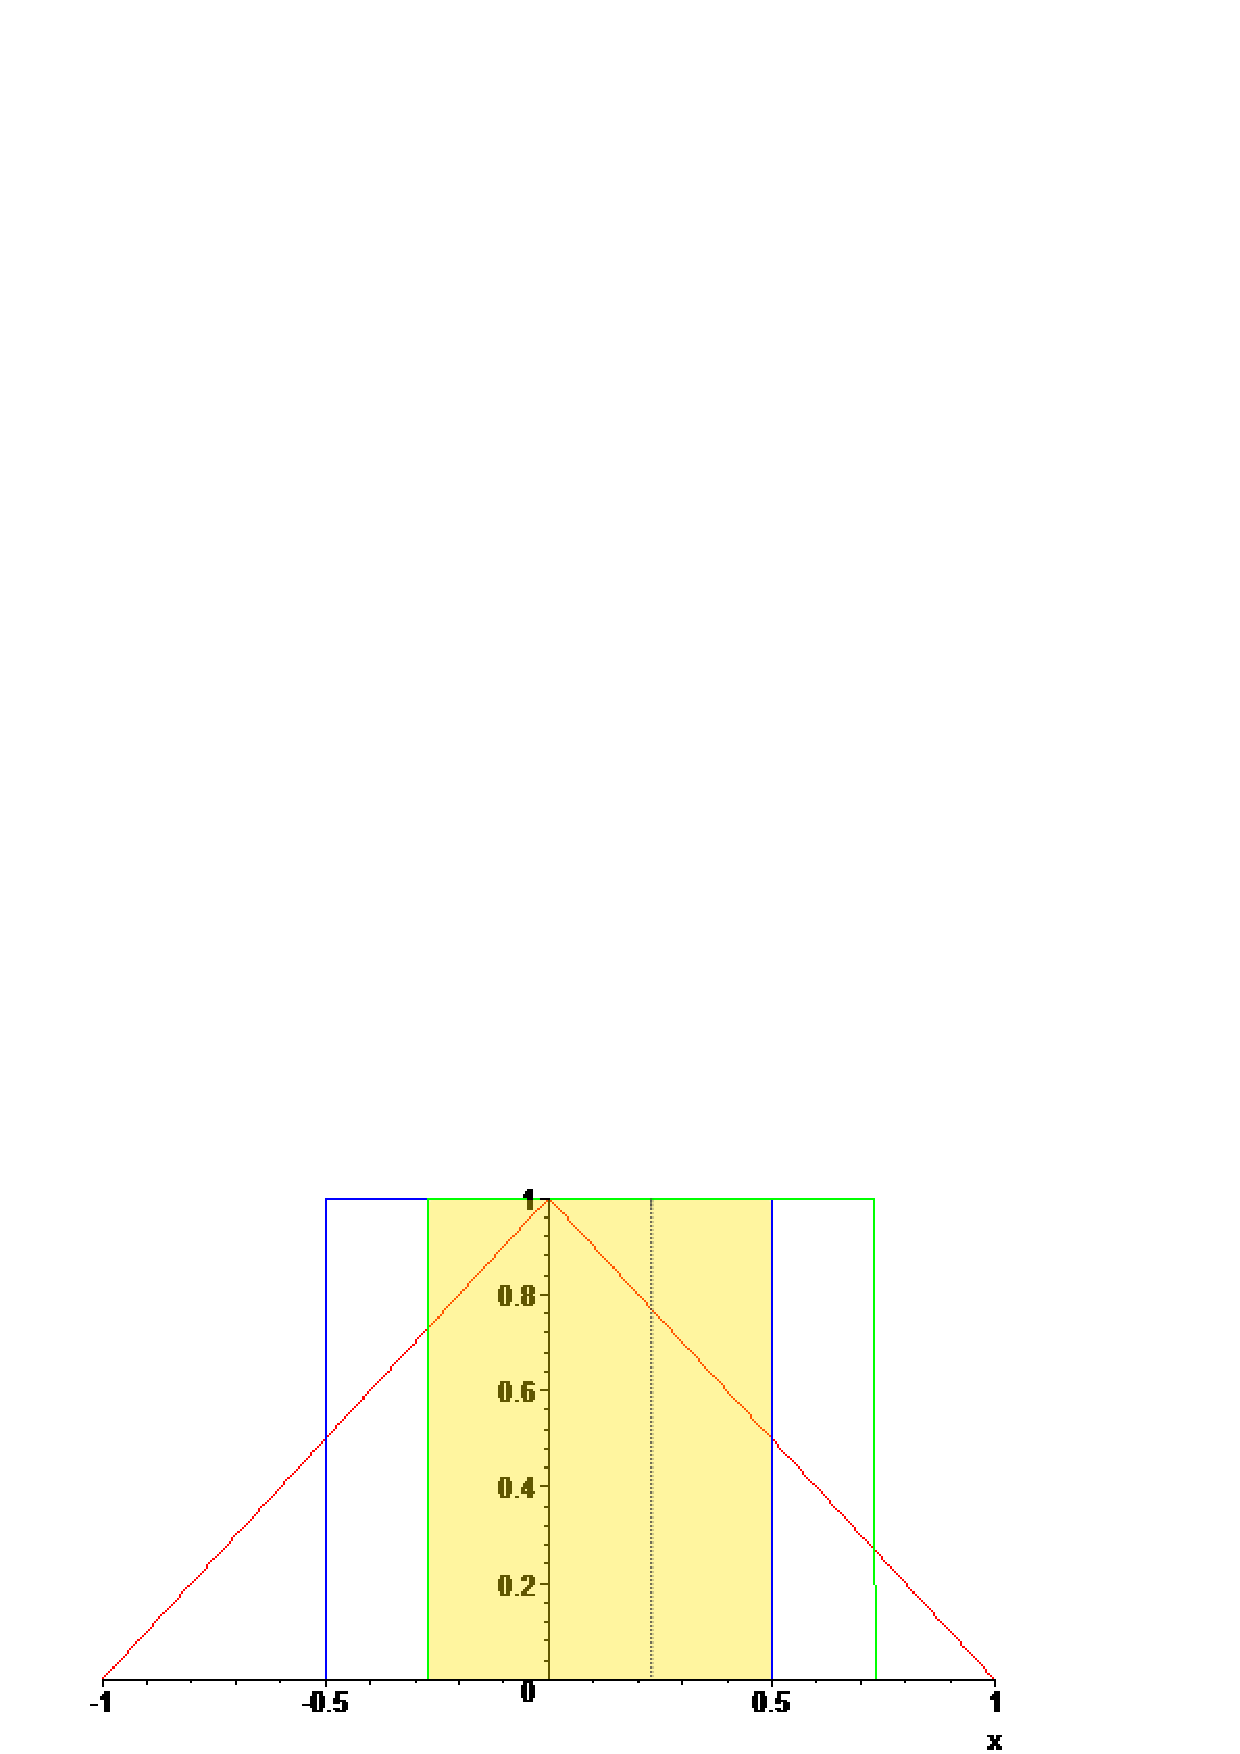
\includegraphics{img/convolution.png}
		\caption{The example of convolution: the rectangle-like function overlaps another, equal rectangle-like function to create a
		triangle-like convolution as the result. In fact - the result is the modified trapezoid for the general case.
		\label{fig:mathematical_convolution}}
	\end{center}
\end{figure}  

Now we are ready to define the Hilbert transform. In fact it is a convolution of given function $f(x)$ with the function $h(x) =
\frac{1}{x \, \pi}$. The Hilbert transform has been presented in the equation~(\ref{eq:mathematical_hilbert})

\begin{equation} \label{eq:mathematical_hilbert}
	\mathcal{H}[f(x)] \stackrel{\mathrm{def}}{=}
	 \ \dashint_{ - \infty }^{\infty } f(\omega) \, h(x - \omega) \, d\omega 
	=\ \frac{1}{\pi} \dashint_{ - \infty }^{\infty } \frac{f(\omega)}{(x - \omega)} \, d\omega . 
\end{equation}

It is important to stress that the dashed integral: $\dashint$ used in the equation~(\ref{eq:mathematical_hilbert}) means the Cauchy
principal value integral. It is the integration method for certain improper integrals like $h(x) =\ \frac{1}{x \, \pi}$. The Cauchy
principal value was designed to omit the singularity and it is a less rigorous integration method than the Riemann integral. For the example
singular $ h(x) $ it is defined as in the equation (\ref{eq:mathematical_cvp}):

\begin{equation} \label{eq:mathematical_cvp}
	\dashint_{ - \infty }^{\infty } \frac{f(\omega)}{(x - \omega)} \, d\omega = \lim_{a \to \infty}\,\int_{ - a}^{a }
	\frac{f(\omega)}{(x - \omega)} \, d\omega . 
\end{equation}

More information about the Cauchy principal value integral can be easily found in the literature \cite{henrici_applied}.

We have presented several pairs of functions and their Hilbert transforms in the
Table~(\ref{tab:mathematical_hexample})~\cite{weisstein_hilbert}.

\begin{table} 
  \centering
  \begin{tabular}{c | c}
    \hline \hline    
      $ f(x) $             & $ \mathcal{H}[f(x)] $ \\ 
    \hline \hline 
      $ sin(x) $           & $ cos(x) $ \\ 
    \hline
      $ cos(x) $           & $ - sin(x) $ \\ 
    \hline
      $ \frac{1}{1+x^2} $  & $ - \frac{x}{1 + x^2} $ \\ 
    \hline
      $ e^{-x^2} $         & $ e^{-x^2} \, \frac{ - 2 }{\sqrt{\pi}} \int_{0}^{x} e^{t^2} \, dt$ \\ 
    \hline
      $ \frac{sin(x)}{x} $ & $ \frac{cos(x)-1}{x} $ \\ 
    \hline
      $ \Pi(x) \equiv % case equation of the rectangle function
      \begin{cases} 
       0 \, \text{for}\, |x| > \frac{1}{2} \\
       \frac{1}{2}\, \text{for} |x| = \frac{1}{2} \\
       1\, \text{for}\, |x| < \frac{1}{2}
      \end{cases}        $ & $ \frac{1}{\pi} ln \Bigg{|} \frac{x - \frac{1}{2}}{x + \frac{1}{2}} \Bigg{|}  $ \\ 
    \hline
      $ \delta(x) \equiv \frac{1}{\pi} \, \lim_{\epsilon \to 0} \frac{\epsilon}{x ^ 2 + \epsilon ^ 2} 
                         $ & $ - \frac{1}{\pi \, x} $ \\
    \hline  
  \end{tabular} 
  \caption{The table presents example pair of functions with their Hilbert transforms.}
  \label{tab:mathematical_hexample}
\end{table}

\subsection{Fourier transform and its application}
 
In this thesis we will very often use the description of a function in the time or in the frequency domain. The Fourier transform is a
mathematical translation tool between those two domains and therefore is has many applications in modern physics and of course in optics.

Let $f : \mathbb{R} \to \mathbb{R} $ be a function of time. We can also call this function a signal. When we will search for the frequency
function, also named the frequency spectrum, we can apply the Hilbert transform on the time-domain $ f $ function: $ \mathcal{H}[f(t)] = 
\overarc{f}(\omega) $.

The one-dimensional Fourier transform is defined in the equation~(\ref{eq:mathematical_fourier}):

\begin{equation} \label{eq:mathematical_fourier}
  \overarc{f}(\omega) = \mathcal{F}[f(t)] \stackrel{\mathrm{def}}{=} \int_{- \infty} ^ {\infty} f(t) e ^{-2 \pi i t \omega} \, dt .
\end{equation}

We will also use the inverse Fourier transform as defined in the equation~(\ref{eq:mathematical_invfourier}):

\begin{equation} \label{eq:mathematical_invfourier}
  f(t) = \mathcal{F}^{-1}[\overarc{f}(\omega)] \stackrel{\mathrm{def}}{=} \int_{- \infty} ^ {\infty} \overarc{f}(\omega) e ^{-2 \pi i
  \omega t} \, d\omega .
\end{equation}

A typical example of a implemented Fourier transform can be find in the typical radio display called the equalizer as in the
Figure~(\ref{fig:mathematical_equalizer}).

\begin{figure} 
	\begin{center}
 		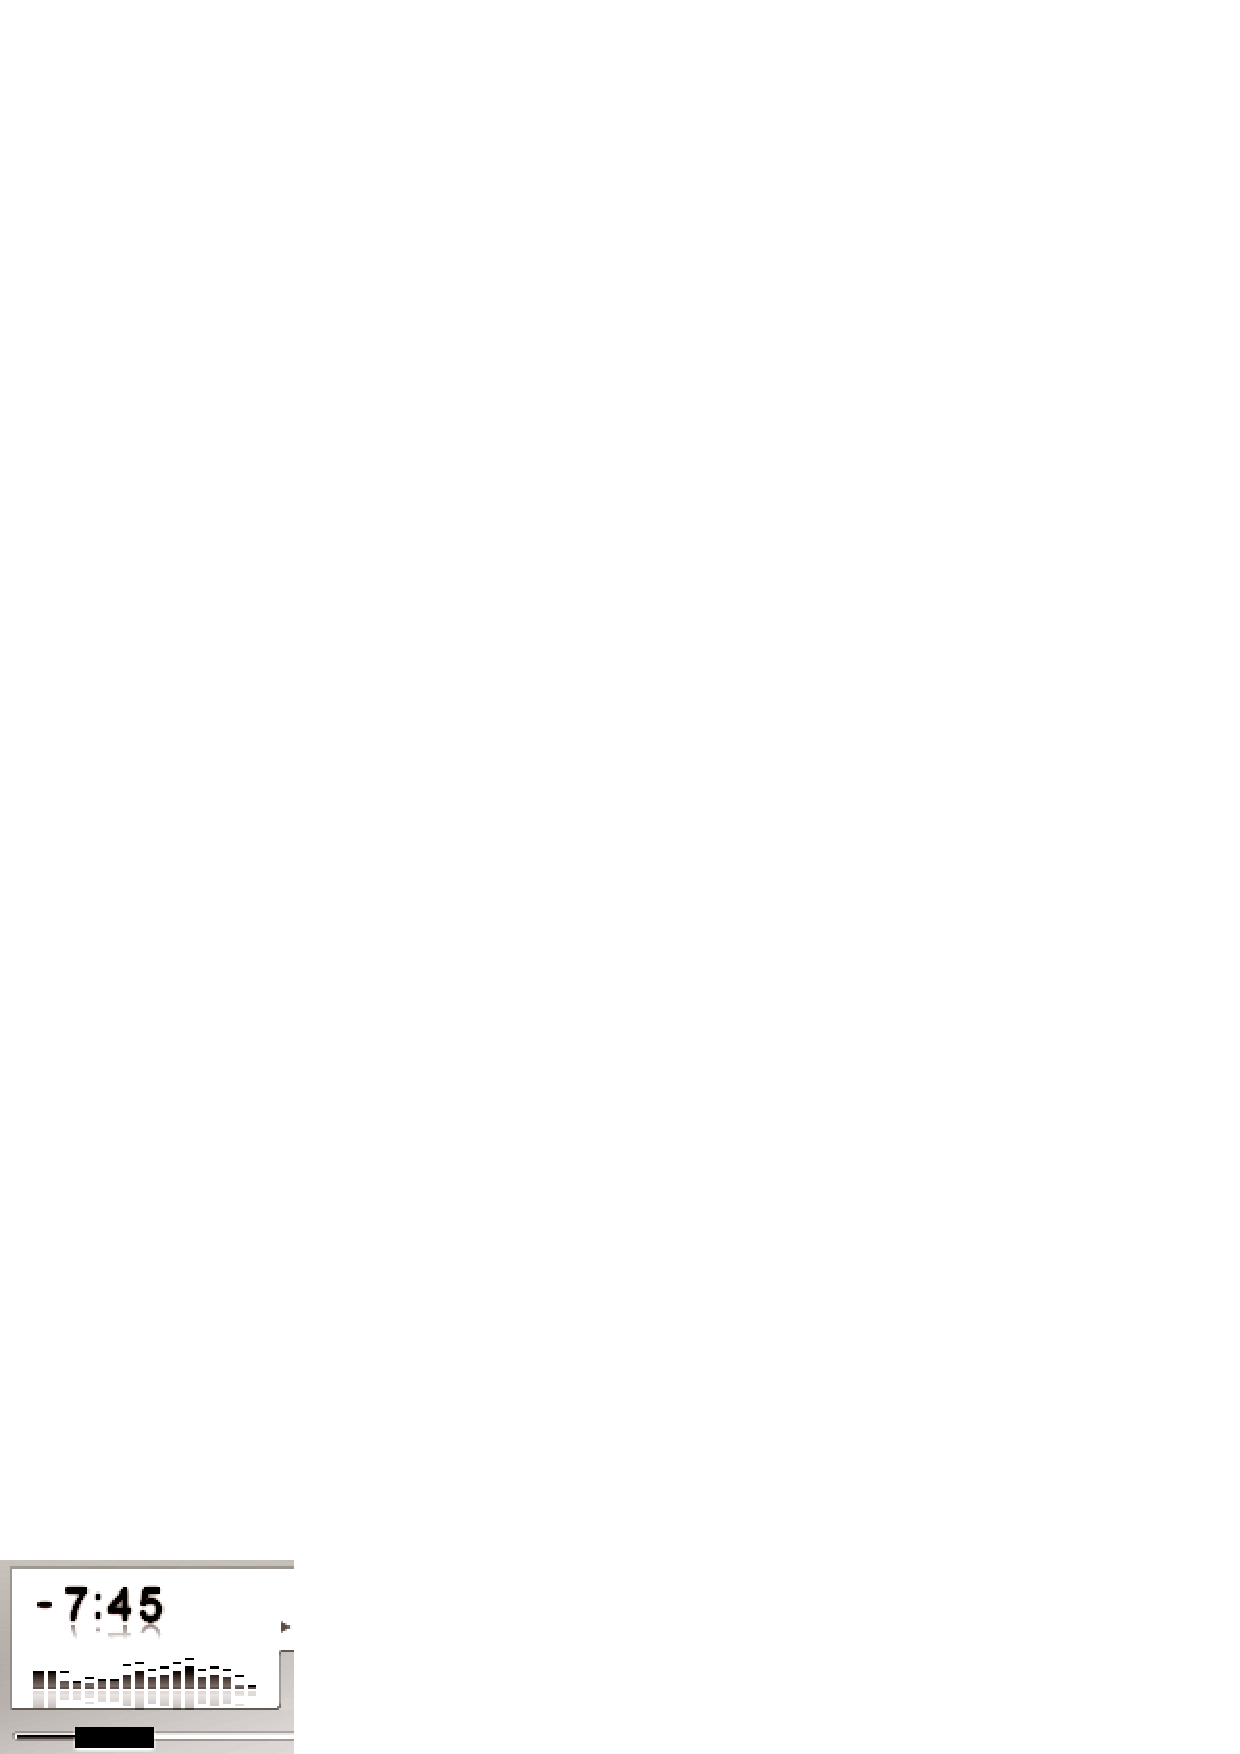
\includegraphics[width=60mm]{img/equalizer.png}
 		\caption{The typical radio display - showing the proper wavelengths used in the current fragment of a music track.
 		\label{fig:mathematical_equalizer}}
	\end{center}
\end{figure} 

The sound wave behaves in a similar way to the the light wave. We can investigate properties of a light in the time domain - but we can also
ask a question what different wavelengths is the investigated light beam created of. We will easily find the Fourier transform a good
mathematical tool for answering such question. More information about the Fourier transform and its application can be easily found in the
literature, for instance in Trott~\cite{trott_mathematica}.

\subsection{Lebesgue and Hardy spaces}

We shall also define the Lebesgue and the Hardy spaces for the next calculations. The Lebesgue space is also called the $L^p$ and is a
function space described in the functional analysis. We can now define a function $f : \mathbb{S} \to \mathbb{D}$. The function $f$ belongs
to the $L^p$ space if it is measurable and if raised to the $p^{\text{th}}$ power it has a finite integral on $\mathbb{S}$ with the measure
$ \mu $. The formal definition has been presented in the equation~(\ref{eg:mathematical_lebesgue}):

\begin{equation} \label{eg:mathematical_lebesgue}
  \|f\|_p \equiv ( \int_{S} |f|^p \, d\mu) ^ {\frac{1}{p}} < \infty .
\end{equation}

Instead of $\mathbb{S}$ we will often use the set of real numbers. The $L^2$ space, also named the set of quadratically integrable functions
is commonly used in physics. When we have the frequency domain of a light signal it must belongs to the $L^2$ space. Otherwise its energy would
be considered as infinite. The Hardy spaces are a part of research interests in the complex analysis. They can be defined on domains like
discs or circles, but they can also be defined for domains like the upper-half plane. We will take a closer look only for the third case.

The upper-half plane $ \mathbb{H} $ is the set of complex numbers defined as in equation (\ref{eq:mathematical_upperhalfplane}):

\begin{equation} \label{eq:mathematical_upperhalfplane}
  \mathbb{H} = \{ x + i \, y \;| y > 0; x, y \in \mathbb{R} \} .
\end{equation}

The complex analysis very often investigates properties of the holomorphic functions. We say a function $f : \mathbb{C} \to \mathbb{C}$ is
holomorphic when it has a complex derivative in each point of its domain and also in a small neighbourhood for each of domain points. For
the complex function $f$ the complex derivative is defined with a limit - very similar as for the real function - as in equation
(\ref{eq:mathematical_complexderivative}):

\begin{equation} \label{eq:mathematical_complexderivative}
  f(z_0)^{'} \stackrel{\mathrm{def}}{=} \lim_{z \to z_0} \frac{f(z) - f(z_0)}{z - z_0} \; \, \text{ and } \, z_0, \, z \in \mathbb{C} .
\end{equation}

The Hardy space $ H^{p} $ defined on the upper-half plane $ \mathbb{H} $ is a class of holomorphic functions for which the norm $
\|f\|_{H^p} $ is finite. The required norm satisfies the equation (\ref{eq:mathematical_hardynorm}):

\begin{equation} \label{eq:mathematical_hardynorm}
  \|f\|_{H^p} = sup_{ y > 0 } \left[ \int |f(x + i \, y)|^{p} \, dx \right]^{\frac{1}{p}} \, < \, \infty.
\end{equation}

\subsection{The causality principle} \label{chap:mathematical_causality}

The causality is the important hypothesis not only in physics, but also in philosophy and statistics. Causality in physics links the cause
with its effect. The first and easy example can be a force acting on a mass. The mass starts to accelerate because of the applied force.
Therefore the force is here the cause and the mass acceleration is the effect.

In the field of optical research - we will be interested in both light and matter properties. When a light signal is passing through a
matter, from the time-domain perspective - we can extract the input and the output signals, as presented on Figure
(\ref{fig:mathematical_inoutput}). From now on we will consistently use the \textbf{input} definition for the time-domain signal in time
period \textbf{before} the interaction with the investigated matter and the \textbf{output} definition for the the time-domain signal
\textbf{after} the interaction with matter.

 We must have in our mind, that not only in the field of optics some scientists creates the models which does not obey
 causality~\cite{mukamel_causal}. But in this thesis we will assume the causality applies to all models being investigated by us.

\begin{figure} 
  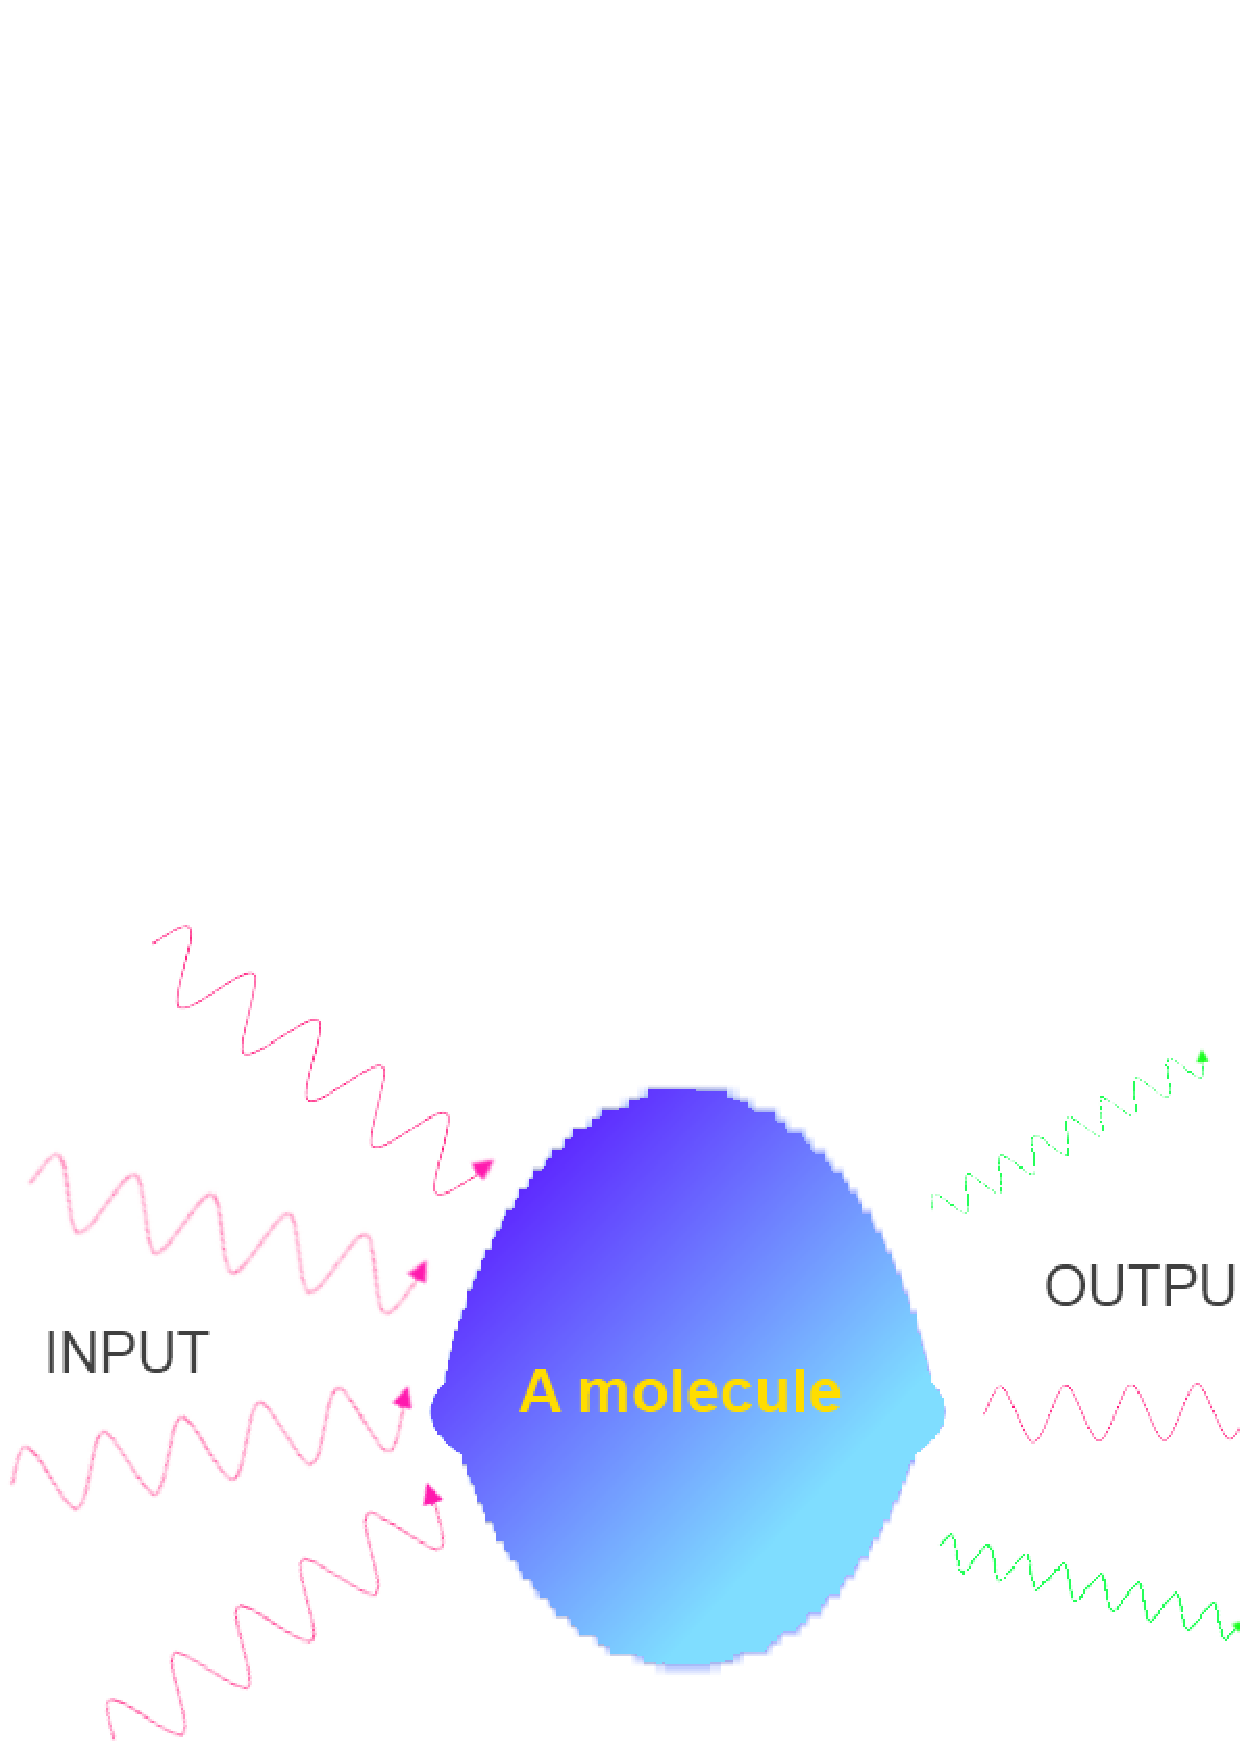
\includegraphics[width=150mm]{img/opt_phenom3.png}
  \caption{Schematic diagram of the nonlinear phenomenon -- the input beam(s') wavelength(s) may differ from the output signal(s).
  This happens only in case of the strong optical signals.
  \label{fig:mathematical_inoutput}}
\end{figure}

\subsection{The Titchmarsh theorem}

The central theorem in this thesis is the Titchmarsh theorem. It links the Fourier transform with the causality principle. We will focus on
the output signal $ a(t) : \mathbb{R} \to \mathbb{R} $ and assume that the interaction with matter happens in the $ t = 0 $ time, but the
interaction time is negligibly short. As the causal output signal - for time $ t < 0 $ it's value equals zero. Our second assumption will be
that the output signal is quadratically integrable. We will also assume that the Fourier transform of the output signal $ \chi(\omega) =
\mathcal{F}[a(t)] \, \in H^2 (\mathbb{H}) $ belongs to the Hardy space of the second order in the upper-half plane $ \mathbb{H} $. With such
assumptions the Titchmarsh theorem states for the $ \chi $ function that it's real and imaginary values are Hilbert transform of each other.

We have prepared the more formal notation of the Titchmarsh theorem in the following equations:

\textbf{We assume that:}
 
\begin{equation} \label{eq:mathematical_l2output}
  a(t) \in L^{2} (\mathbb{R}),
\end{equation}
\begin{equation} \label{eq:mathematical_faoutput}
  \text{For all } \, t < 0 \, \text{ : } \, a (t) = 0,
\end{equation}
\begin{equation} \label{eq:mathematical_ttisfourier}
  \chi(\omega) = \mathcal{F}[a(t)],
\end{equation}
\begin{equation} \label{eq:mathematical_tth2fourier}
  \chi(\omega) \in H^2(\mathbb{H}).
\end{equation}

\textbf{The Titchmarsh theorem states that:}  

\begin{subequations}  \label{eq:mathematical_titchmarsh_relations}
  \begin{equation} \label{eq:mathematical_titchmarsh_real}
    \Re (\mathrm{\chi}(\omega )) =  \frac{1}{\pi}\,\dashint_{ -\infty }^{\infty }
    \frac {\Im (\mathrm{\chi}(\Omega ))}{\Omega - \omega }\,d\Omega , 
  \end{equation}
  \begin{equation} \label{eq:mathematical_titchmarsh_imag}
    \Im (\mathrm{\chi}(\omega )) = -\frac{1}{\pi}\,\dashint_{ -\infty}^{\infty }
    \frac {\Re (\mathrm{\chi}(\Omega ))}{\Omega - \omega }\,d\Omega .
  \end{equation}
\end{subequations}

The Titchmarsh theorem states that the conditions from equations~(\ref{eq:mathematical_l2output} with~\ref{eq:mathematical_faoutput}),
(\ref{eq:mathematical_ttisfourier} with~\ref{eq:mathematical_tth2fourier}) and~(\ref{eq:mathematical_titchmarsh_real} with
\ref{eq:mathematical_titchmarsh_imag}) are mathematically equivalent.

Proof with an exhausting review of both the Fourier and Hilbert transforms was described by Edward Charles Titchmarsh in
\cite{titchmarsh_introduction} - the theory is described through all book chapters, but the theorem and its proof has been stated in Chapter
(\ref{chap:nc}) about the conjugated integrals also Hilbert transforms.


\section{Physical models to be used} \label{chap:physical_models}

\subsection{The linear and the nonlinear optics} \label{chap:physical_linearnonlinear}

From now on we will focus on the application of the Hilbert transform in the optical research. The central interest of the optical research
is the interaction of light and matter. 

The light, also called the electromagnetic radiation, is a form of energy which travels between particles in a wave manner. From the
microscopic point of view, light is also a beam of photons. The photon is the elementary massless particle that transport the special
quantities of energy. The energy $E$ of a single photon is inversely proportional to its wavelength $\lambda$ as described in the equation
(\ref{eq:photon_frequency}). The $h = 4.135667516(91) \times 10^{-15} eV \cdot s$ is the Planck constant and the $c = 299792458 \frac{m}{s}$
is the speed of light:

\begin{equation} \label{eq:photon_frequency}
	E(\lambda) = \frac {h\,c} {\lambda}.
\end{equation}

When the light interacts with matter the energy transfer occurs. If the light or more precisely the photon is absorbed - the matter
increases its energy by the quantum of energy transported by that photon. When the light is emitted, some portion of the matter's energy is
converted into a newly generated photon. In the optical research we are interested in both processes - the absorption and the generation of
light. We are also interested in the theory behind these two effects - which will help us understand the nature of light in general. The
good introduction into the theory of optics can be found in the McGraw-Hill encyclopedia~\cite{mcgraw_encyclopedia}, starting from the~$
12^{\text{th}} $ volume.

Optics is divided in the main two areas - the linear and the nonlinear optics. To distinguish linear from the nonlinear phenomena,
we need to remind the superposition. The superposition principle is applied to the linear system and its states the system fulfill the
additivity (\ref{eq:physical_additivity}) and the homogeneity (\ref{eq:physical_homogeneity}) properties. The additivity is a term taken
from algebra and it describes the function~$ f : \mathbb{X} \to \mathbb{Y}$ that preserves the addition operation:

\begin{equation} \label{eq:physical_additivity}
  \forall x, y \in X : f(x + y) = f(x) + f(y) .
\end{equation}

The homogeneity is an algebraic property of a function $f$: if the argument $x \in \mathbb{X} $ of a function $f : \mathbb{X} \to \mathbb{Y}
$ is multiplied by a scalar $ \alpha $ the result is also multiplied by this scalar. More precisely:

\begin{equation} \label{eq:physical_homogeneity}
  \forall \alpha \in \mathbb{R} \, \text{ and } \, \forall x \in \mathbb{X} : f(\alpha \, x) = \alpha \, f(x) .
\end{equation}

In the linear optics we state that the system satisfies the superposition principle. ``The system'' here is the investigated setup of light
and matter. From the microscopic point of view it means - the more often photons transfers energy to and from the mass, the more the same
effects take place and the only difference is the amount of energy being transferred in the set period of time. When the systems starts to
``saturate'', photons cannot be processed in the same way and some new optical phenomena take place.

\subsection{The response of a system} \label{chap:physical_systemresponse}

To better understand the relation between the light~\textbf{input} and~\textbf{output} we shall once more use the convolution.
Given the input signal in the time-domain: $ x(t) $ and the linear systems response function described as $ h(t) $ we can easily get the
output signal $ y(t) $ as the convolution $ x(t) \convolution h(t) $:

\begin{equation} \label{eq:physical_response}
  y(t) = x(t) \convolution h(t) \stackrel{\mathrm{def}}{=} \int_{ - \infty}^{ \infty} x( t - \tau ) \cdot h(\tau) \, d\tau .
\end{equation}

This definition gives no new information because we now nothing about the response function $ h(t) $. But from the convolution
theorem~\cite{katznelson_introduction} we know that the Fourier transform applied to the convolution of two given functions equals the
simple multiplication of two Fourier transforms:

\begin{equation} \label{eq:physical_convolution}
  \mathcal{F}(a(x) \convolution \chi(x)) = \mathcal{F}(a(x)) \cdot \mathcal{F}(\chi(x)) .
\end{equation}

The proof to the convolution theorem (\ref{eq:physical_convolution}) can be found in \cite{titchmarsh_introduction}.

The definition of the system's response (\ref{eq:physical_response}) is true for the linear case. For the nonlinear systems we must provide
the more complicated mathematical tool called the Volterra series model well described in the PhD thesis of Antonín
Novák~\cite{thesis_novak}. The output signal $ y(t) $ equals the sum of components, each of which is the~$ n ^ {\text{th}} $ order Volterra
operator $ \mathbf{K_n} $ of the input signal $ x(t) $:

\begin{equation} \label{eq:physical_volterraseries}
  y(t) = \sum_{n} \, \mathbf{K_n}[x (t) ].
\end{equation}

The $ n ^ {\text{th}} $ order Volterra operator $ \mathbf{K_n} $ is defined as the multidimensional convolution:

\begin{equation} \label{eq:physical_volterraoperator}
  \mathbf{K_n} = \int_{ - \infty}^{\infty} \ldots \int_{ - \infty}^{\infty} k_n (\tau_1, \ldots, \tau_n) \, \cdot \, x(t - \tau_1) \, \ldots
  \, (x - \tau_n)\, d\tau_1 \, \ldots \, d\tau_n .
\end{equation}

The $ k_n : \mathbb{X}^{n} \rightarrow \mathbb{Y} $ function is called the $ n ^ {\text{th}} $ order Volterra-kernel. 

We notice the output function for the linear case (\ref{eq:physical_response}) is equal to the nonlinear output function assuming that all
the Volterra-kernels of orders higher than one are equal to zero. We say the kernel is causal if it equals zero for any negative
argument.

From now on we must distinguish the light~\textbf{input}, the light~\textbf{output} and the matter~\textbf{response} functions from each
other. The matter~\textbf{response} function for the interaction of the $ n^{\text{th}} $ order is the $ n^{\text{th}} $ order
Volterra-kernel.

\subsection{The linear system} \label{chap:physical_linearsystem}

Let imagine an input single pulse-like signal ``shots'' the matter. We expect the matter to response with a short, fading response signal.
The $ \Theta (t) : \mathbb{R} \rightarrow \{0, \, 1 \} $ function will state the Heaviside function defined as in the equation
(\ref{eq:physical_heaviside}):

\begin{equation} \label{eq:physical_heaviside}
   \Theta(t)  =  
   \begin{cases}
     0 \, \text{for} \, t < 0, \\
     1 \, \text{otherwise}.
   \end{cases}
\end{equation}

Not getting into the theory of the linear optical response, we can create our first simple response function $ h_{\text{lin}} $ as the
fading sinusoidal exponent:

\begin{equation} \label{eq:physical_linear_response}
  h_{\text{lin}} (t) = 1 - e^{( - t)}\,\mathrm{sin}(20\,t)\,\Theta (t) .
\end{equation}

The plot of the equation (\ref{eq:physical_linear_response}) is given on Figure (\ref{fig:physical_linplot}).

\begin{figure}[H]
  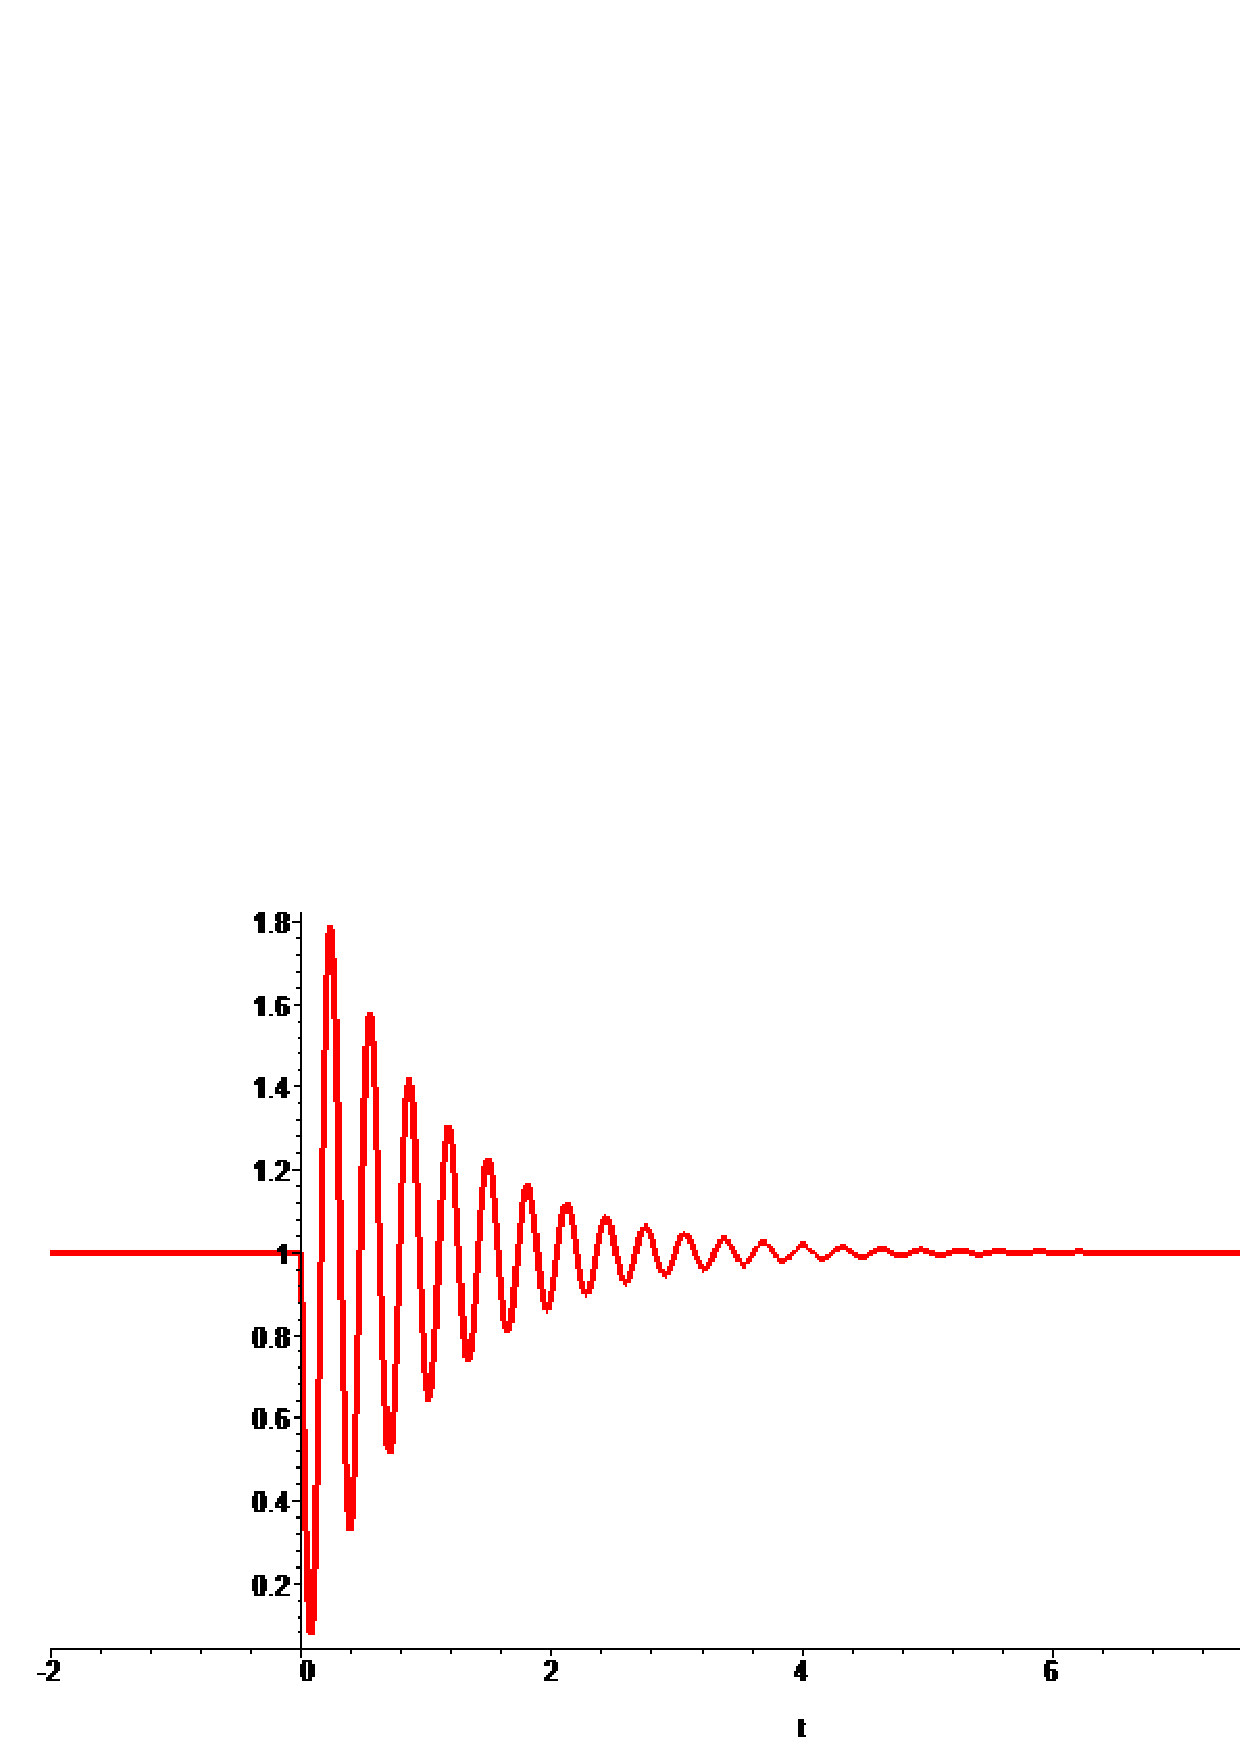
\includegraphics[width=150mm]{img/lin_plot.png}
  \caption{A typical linear response signal in time domain \label{fig:physical_linplot}}
\end{figure}

If we would like to know the response signal in the frequency domain, we will apply the Fourier transform on the~$ h_{\text{lin}} $:

\begin{equation} \label{eq:physical_frequency_linear}
  \mathcal{F}[h_{\text{lin}}] = \chi_{\text{lin}}(\omega) \approx \frac{ -20}{(\omega \,i + 1 -20\,i)\,(\omega \,i + 1 + 20\,i)},
\end{equation}

In the equation (\ref{eq:physical_frequency_linear}) we have omitted the Dirac delta function that will appear if we calculate the Fourier
transform properly. The Dirac delta function can be omitted from the numerical point of view. The calculated $ \chi_{\text{lin}} $
is called the linear optical susceptibility. We are interested in the notation of $ \chi_{\text{lin}} $ as the function of frequency
$ \omega $. More theoretical background about the optical susceptibility can be found in Boyd~\cite{boyd_nlo}. 

As You can see - the time domain linear response signal $ h_{\text{lin}} $ and the corresponding linear optical susceptibility~$
\chi_{\text{lin}} $ pass the assumptions of the Titchmarsh theorem. In the further numerical calculations we will put the~$
\chi_{\text{lin}} $ into tests. 

\subsection{Nonlinear models} \label{chap:physical_simnlo}

In this subsection we will shortly describe the time-resolved processes which allow to determine the origin of two important nonlinear
processes: the pump-and-probe and the frequency mixing process.

\subsubsection*{Pump-and-probe process} \label{chap:physical_pnp}

The laser is typically a source of a high-energy input signal. In a typical pump-and-probe process we use two laser beams. One of them
is a strong input and we name it the 'pump'. The second input - the 'probe' - is much less intense. We try to synchronise these two
laser beams in the following way - firstly a pump input hits the matter sample with its strong intensity - causing modifications in the matter
properties. Shortly after that - within a time period $\Delta \, t$ - a low-intensity probe input hits the modified sample and its
properties are measured through a detector. In a typical experiment the $\Delta \, t$ time period should be adjustable. There are various types of
pump-probe experiments, for example one can detect changes of the amplitude of the matter response signal. The schematic diagram of a
pump-and-probe experiment is shown in Figure (\ref{fig:physical_pnp_fig}).

\begin{figure} 
	\begin{center}
		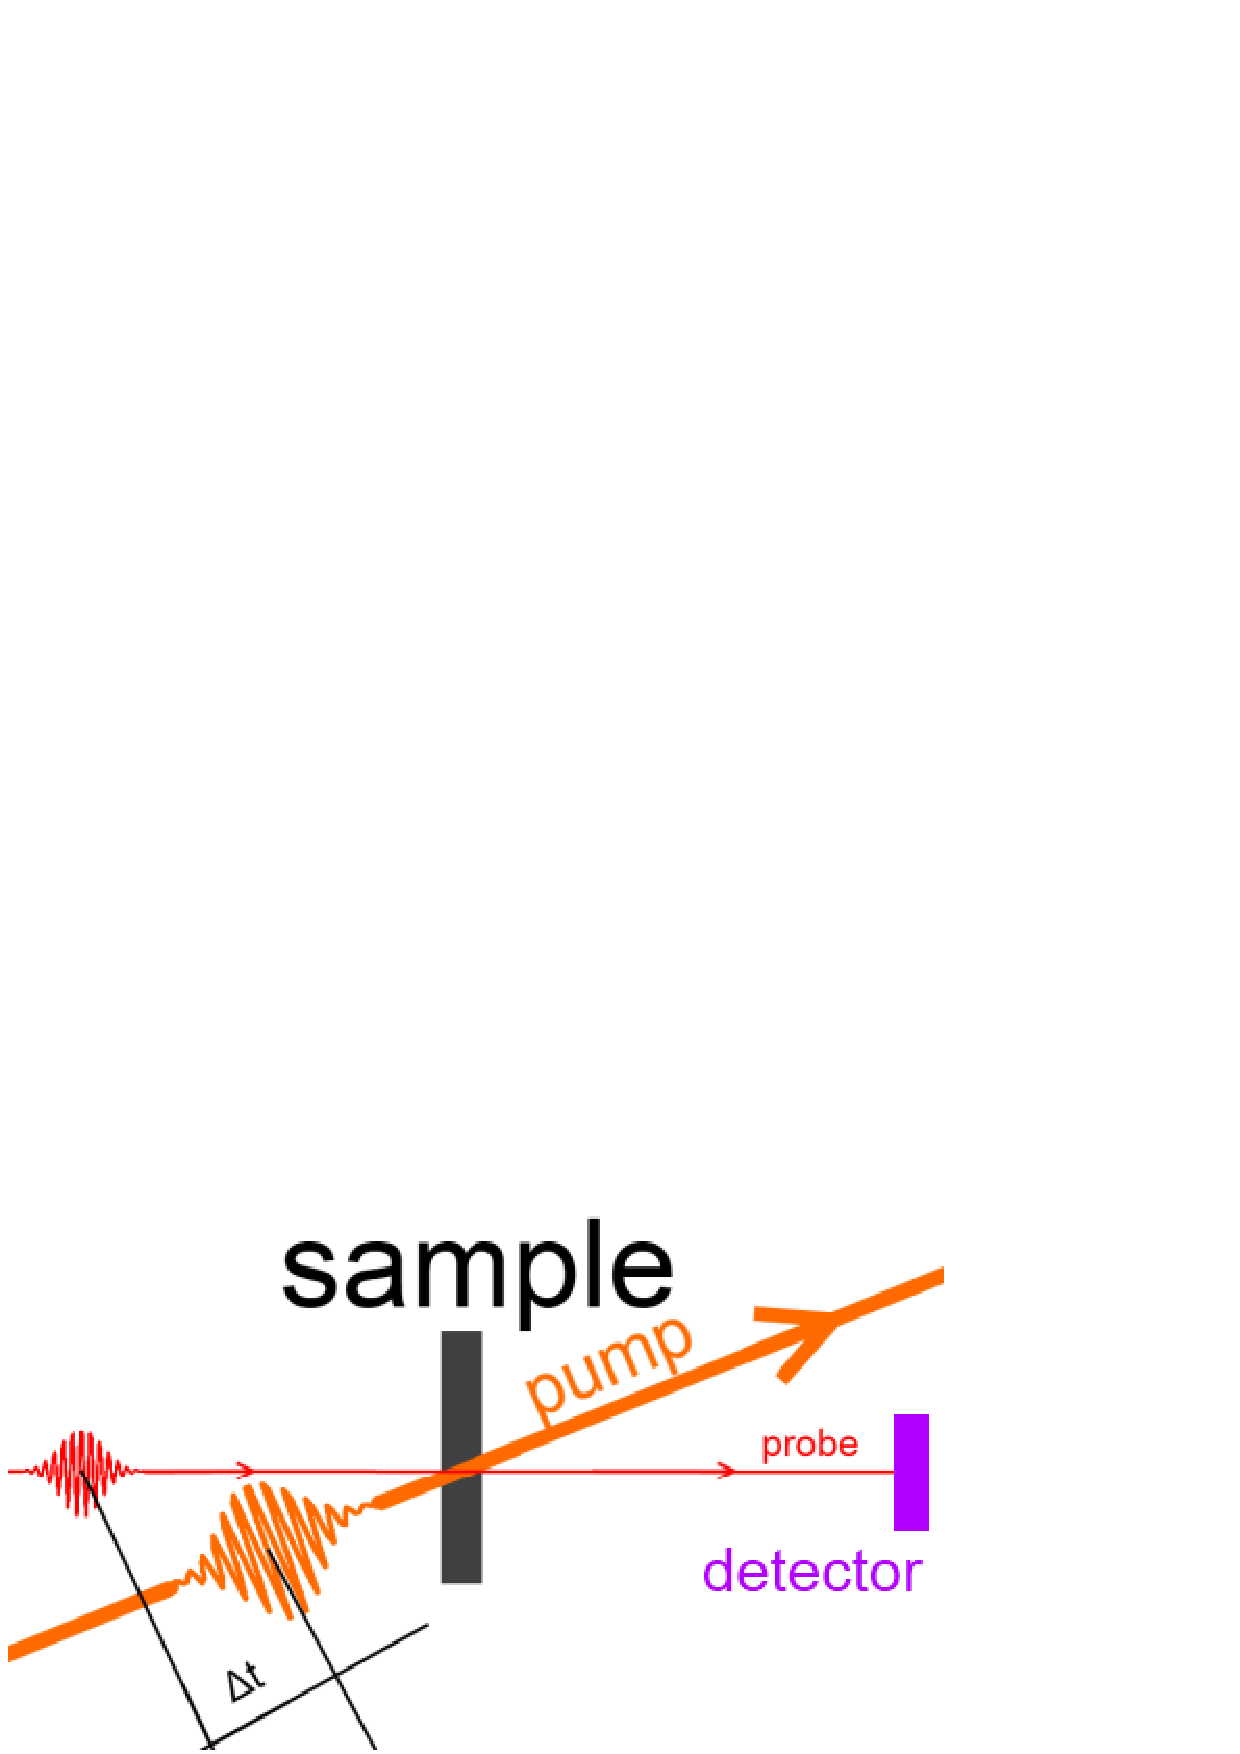
\includegraphics{img/pnp.png}
		\caption{The pump-and-probe experiment\label{fig:physical_pnp_fig}}
	\end{center}
\end{figure}

The key assumption in the pump-and-probe experiment is that separated and independent probe inputs cannot introduce a nonlinear
response of the system alone \cite{boyd_nlo}. The probe signal should be sufficiently weak. In the so-called two-level model the
investigated atomic system is characterized for both the pump and the probe inputs by two different relaxation times:~${T_{1}}$ 
and ${T_{2}}$ respectively. A more detailed model is defined by H. N. Yum et al. \cite{yum_pump} for the nonlinear susceptibility in
case of the pump-probe process:

\begin{multline}   \label{eq:physical_pnp_equation}
     \chi_{pp} (\delta ) = \frac {G\,n^{0}\,{\gamma_{ba}}}{\Delta  + \delta  + i\,\eta } \cdot \\
     [1 - \frac {{\Omega_{1}}^{2}\,(\Delta  - \delta  + i\,\eta )\,(\delta  + 2\,i\,\eta )}{(\Delta  - i\,\eta )\,((\delta  + i\,
     \theta)\,(\Delta  + \delta  + i\,\eta )\,(\delta  - \Delta  + i\,\eta ) - {\Omega_{1}}^{2}\,(\delta  + i\,\eta ))\,2}].
\end{multline}

In the equation (\ref{eq:physical_pnp_equation}) we have introduced a whole branch of new variables. The $\delta $ is the probe
input frequency, the $\Delta $ means the pump input frequency. Other variables are related with the pump $ T_{1} $ relaxation time:

\begin{tabular} {r c l}
	$ \Omega_{1} $  & $ = $ & $ \Omega_{1} ( T_{1} )$, \\
	$ G $           & $ = $ & $  G ( T_{1} )$, \\
	$ n^{0} $       & $ = $ & $  n^{0} ( T_{1} )$, \\
	$ \gamma_{ba} $ & $ = $ & $  \gamma_{ba} ( T_{1} )$, \\
	$ \eta $        & $ = $ & $  \eta ( T_{1} )$, \\
	$ \theta $      & $ = $ & $  \theta ( T_{1} )$, \\
\end{tabular}

The pump relaxation time depends on the time period between $( \Delta_1 \, t)$ input pulses:

\begin{equation} \label{eq:physical_periodtime}
   T_{1} =  T_{1} ( \Delta_1 \, t).
\end{equation}

We can now easily deduce that also the pump-and-probe nonlinear susceptibility depends on the $\Delta_1 \, t $ as presented in the equation
(\ref{eq:physical_pnp_susceptibility}):

\begin{equation} \label{eq:physical_pnp_susceptibility}
  \chi_{pp} = \chi_{pp} (\delta , \Delta_1 \, t).
\end{equation} 

In sense of the response theory this observation leads us to the conclusion, that the susceptibility of the nonlinear process depends not
only on the input signal frequency (energy) - but also on the time delay between the moments, when two or more photons arrive at
the molecule. We are talking about an important problem in nonlinear optics which is constructing a valid model for the pump-and-probe
process - to allow us to use the Titchmarsh theorem. 

In \cite{christodoulides_nonlinear} we can find results showing that the probe signal absorbance depends not only on the pump
signal properties, but also on the time delay between the pump and probe - see Figure (\ref{physical_fig:pnp_absorption}).

\begin{figure} 
	\begin{center}
		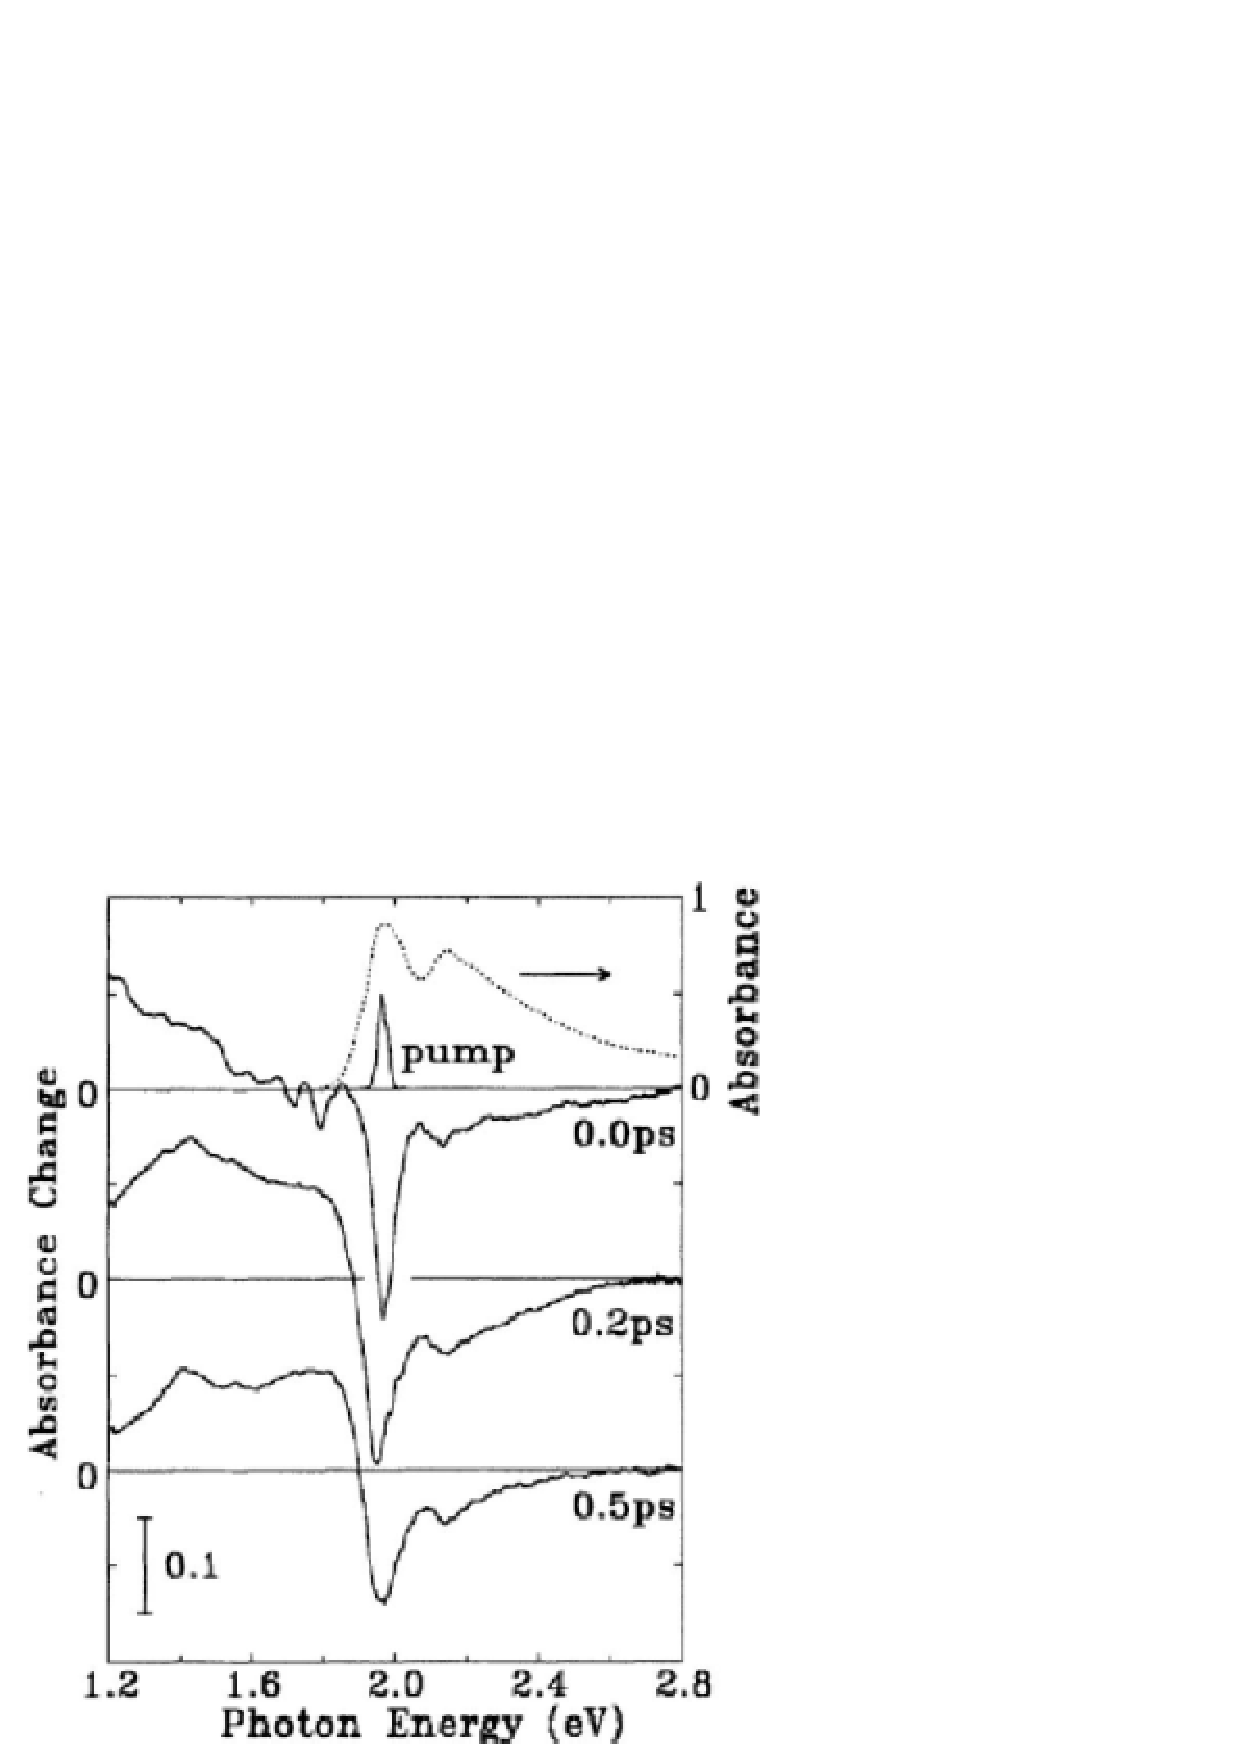
\includegraphics{img/pnp_abs.png}
		\caption{The pump-and-probe absorption change due to time delay between the pump and probe signal. The figure taken from
		\cite{christodoulides_nonlinear}. \label{physical_fig:pnp_absorption} }
	\end{center}
\end{figure}


More interesting results come when we assume that susceptibility is a complex function of two parameters, both the pump and
probe signal frequency:

\begin{equation} \label{eq:pnp_2args}
  \chi_{pp} = \chi_{pp}(\delta, \Delta_1 \, t \, (\text{ const }), \,\Delta )
\end{equation}

Therefore we obtain the three dimensional plots presented on Figures (\ref{fig:physical_pnp_2d}) and (\ref{fig:physical_pnp_3d}).

\begin{figure}
  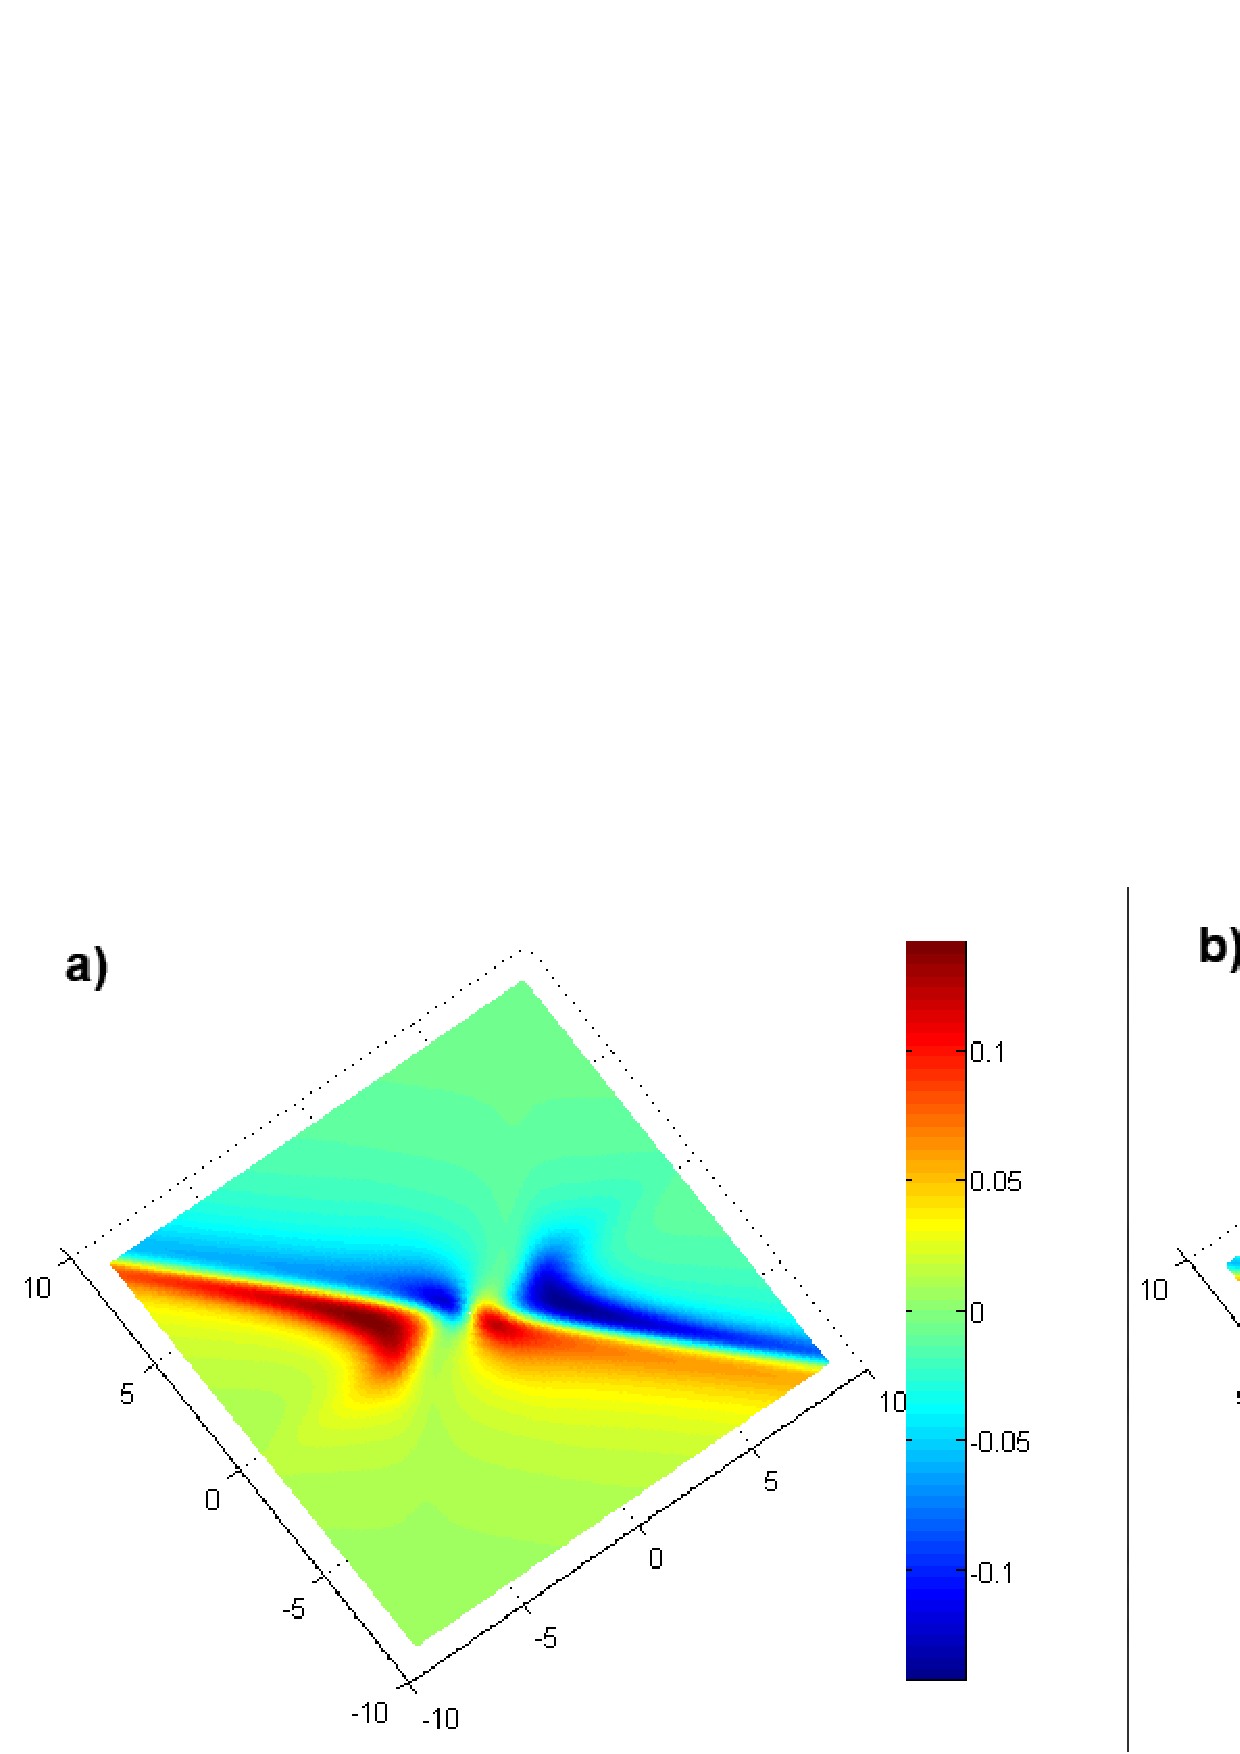
\includegraphics[width=150mm]{img/pnp_2d.png}
  \caption{2-Dimensional plots of both a) real and b) imaginary parts of the nonlinear susceptibility treated as a bi-argumental
  function, where the colour means the function value
  \label{fig:physical_pnp_2d}}
\end{figure}

\begin{figure} 
  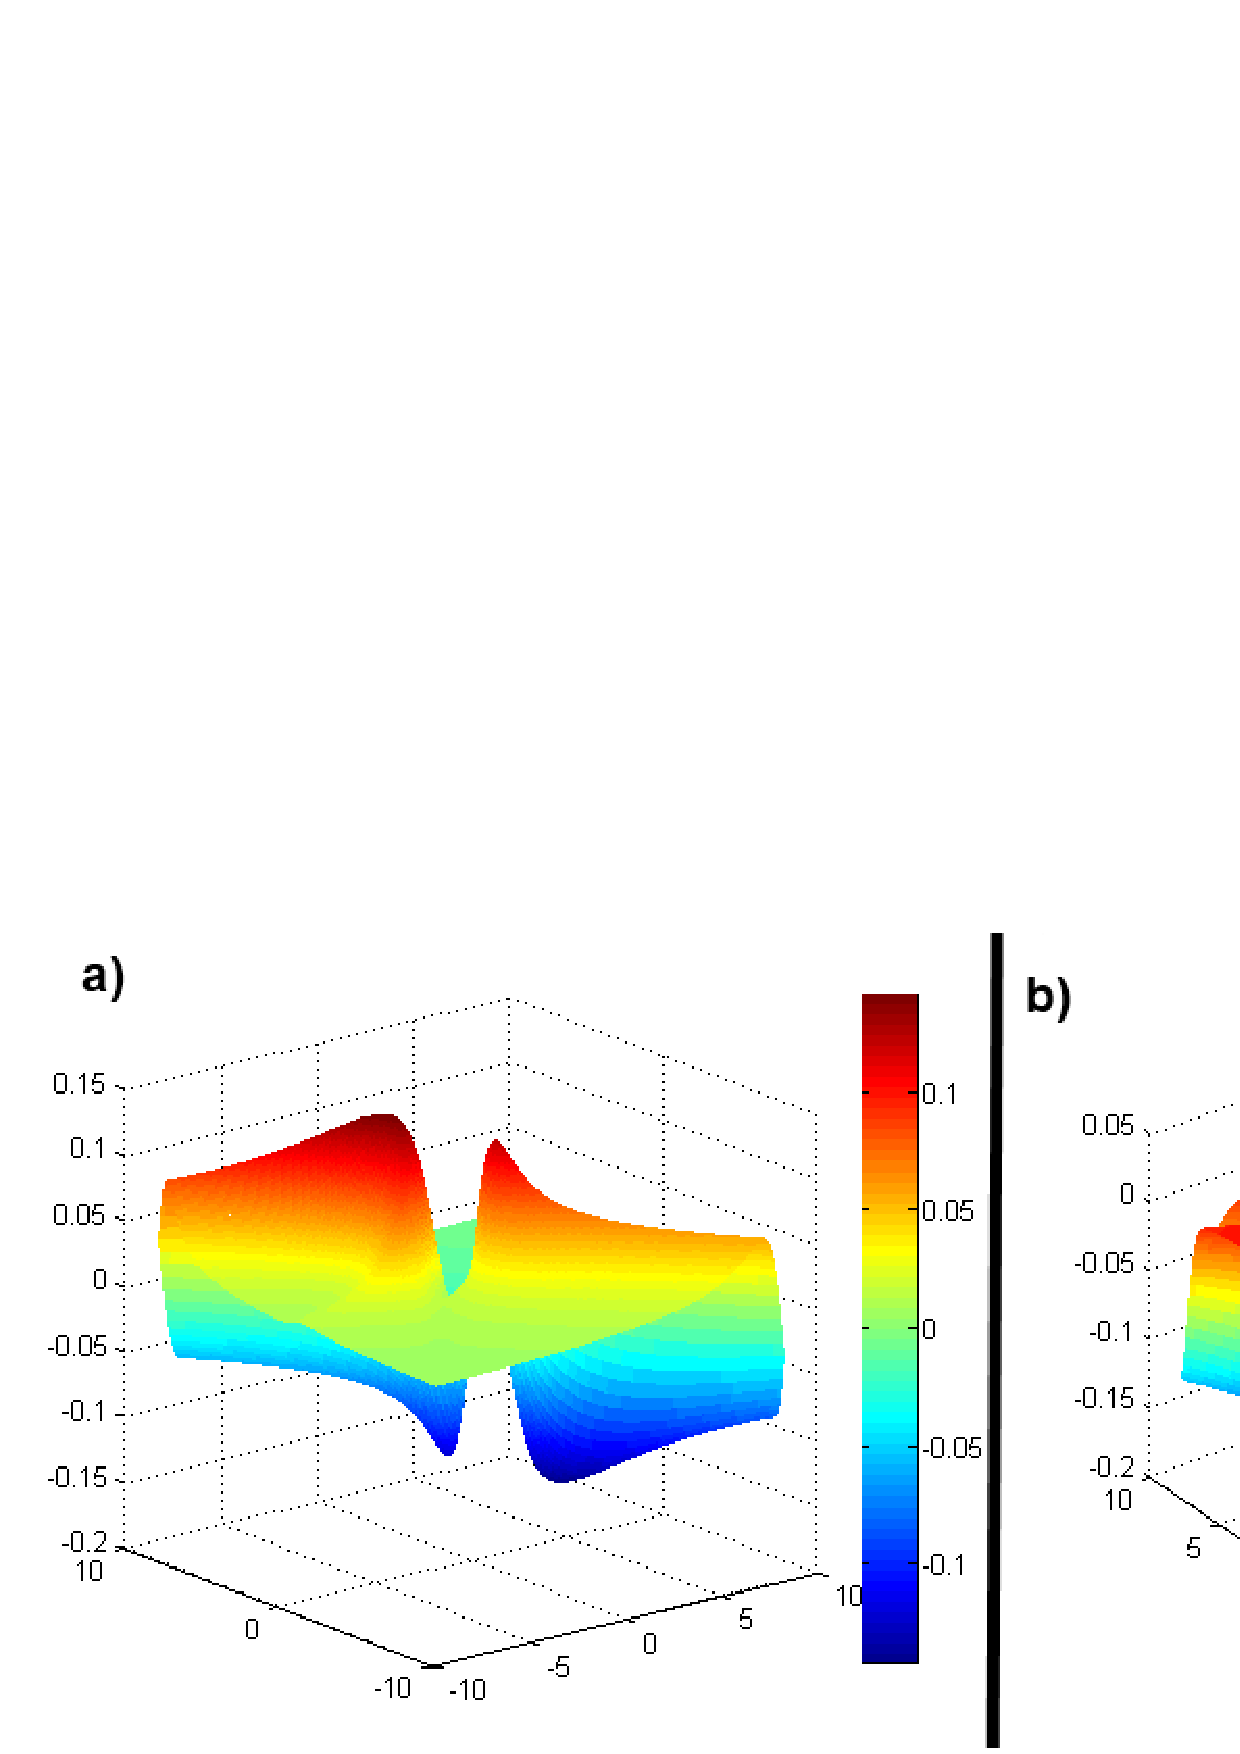
\includegraphics[width=150mm]{img/pnp_3d.png}
  \caption{3-Dimensional plots of both a) real and b) imaginary parts of nonlinear susceptibility treated as a bi-argumental
  function, where the colour means the function value
  \label{fig:physical_pnp_3d}}
\end{figure}


\subsubsection*{Frequency Mixing Process} \label{chap:physical_fm}

The frequency mixing is a general class of processes where we have two or more input photons with their frequencies:
${\omega_{input, \,1}}, \,{\omega_{input, \,2}}, \,{\omega_{input, \,3}}, \ldots $ and we receive one or more output photons with
their frequencies: ${\omega_{output, \,1}}, \,{\omega_{output,\,2}}, \,{\omega_{output, \,3}}, \ldots $. In chapter 6.6 of Boyd
\cite{boyd_nlo} we can find the description of processes in which we use the strong signal 'pump' with frequency $\omega$
and the weak signal 'probe' with the frequency $\omega  - \delta $ nearly copropagating, as it was shown in Figure
(\ref{fig:fmix_sch}).

\begin{figure}
	\begin{center}
		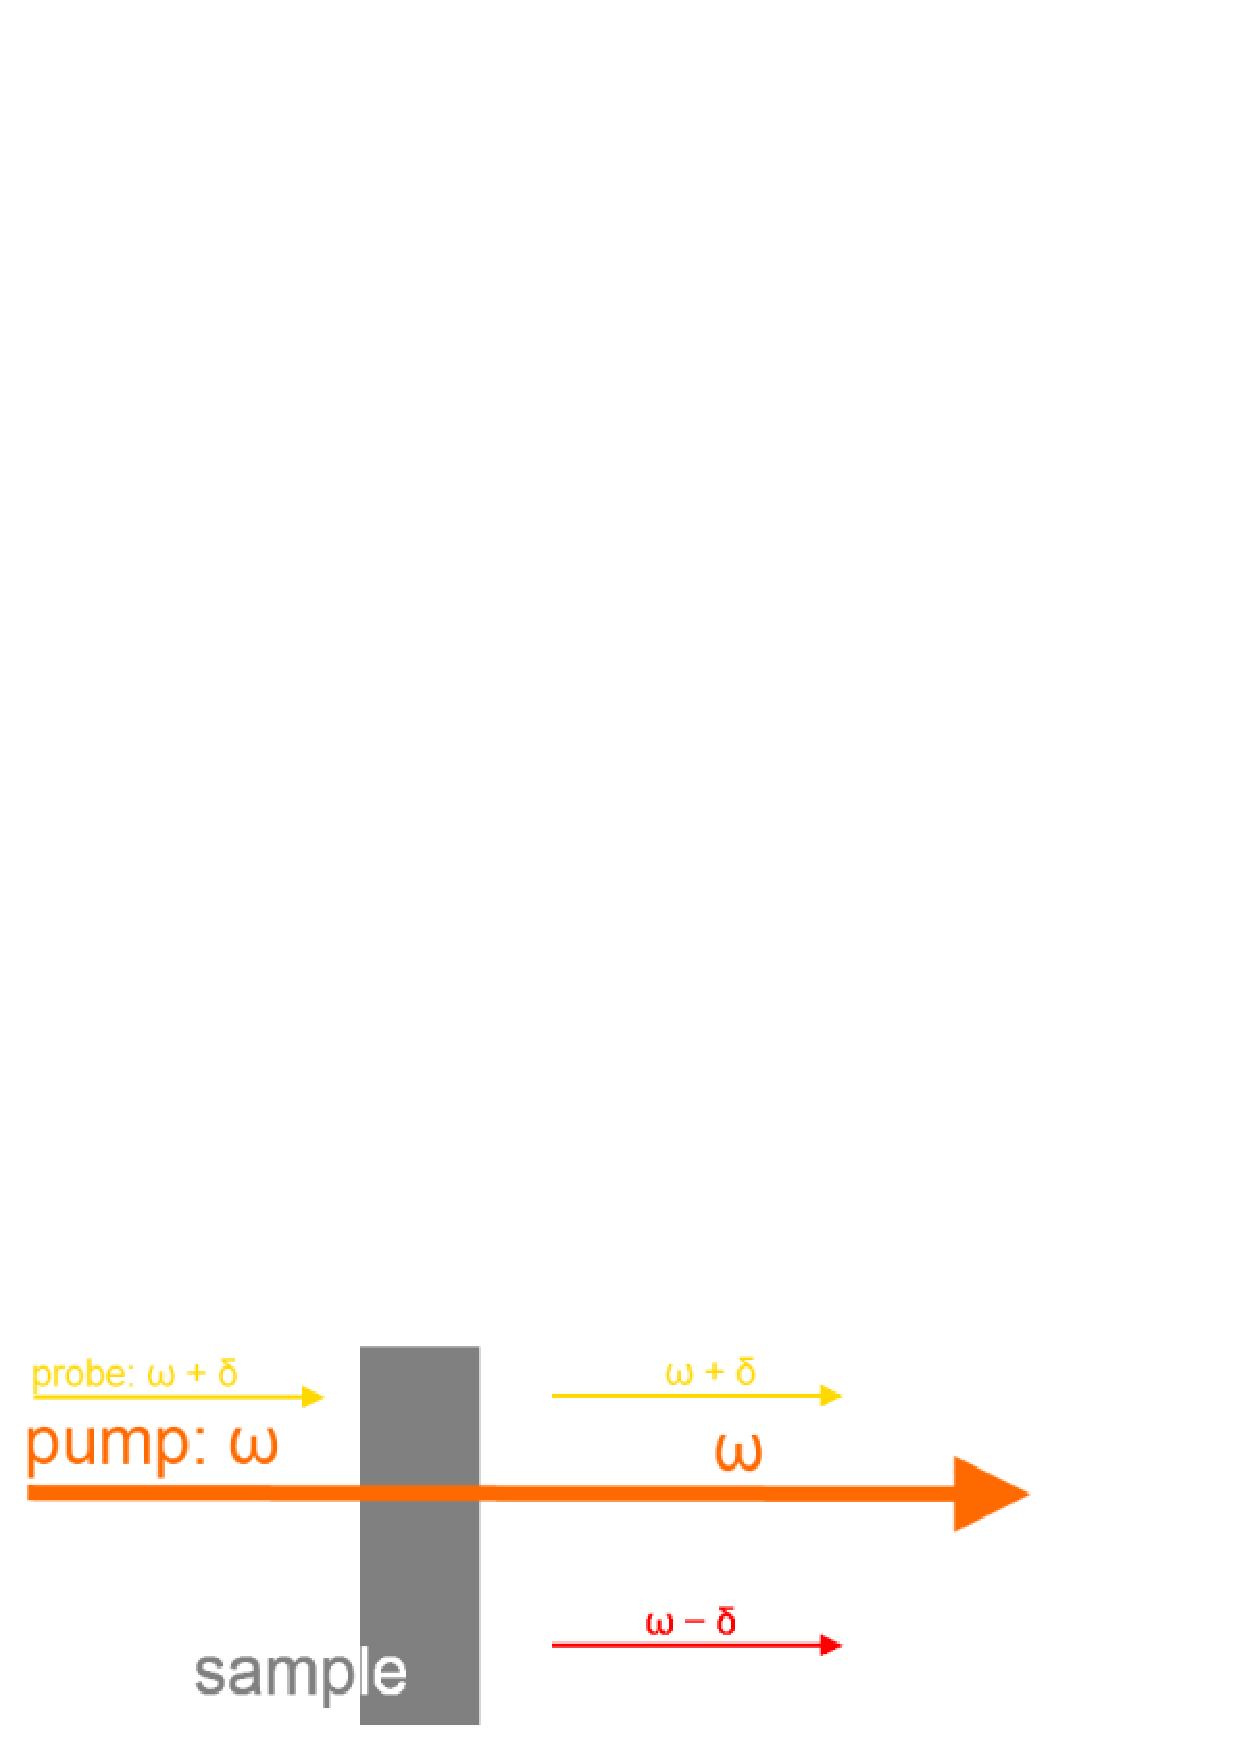
\includegraphics{img/fmix_sch.png}
  		\caption{The pump-and-probe frequency mixing process from chapter 6.6 Boyd \cite{boyd_nlo}. \label{fig:fmix_sch}}
	\end{center}
\end{figure}

For such a process the model for the linear susceptibilities has been defined by Boyd for both $\omega  + \delta $ and $\omega  -
\delta $ frequencies, where $T_1$, $T_2$ and $\Delta$ are time-related variables, assumed constant in this thesis:

\begin{subequations} \label{eq:fmix_eff1}
  \begin{equation}   \label{eq:feff1_plus}
    \chi_{eff, 1}(\omega + \delta, T_1 \text{\tiny{ = const}}, T_2 \text{\tiny{ = const}}, \Delta \text{\tiny{ = const}}) = \frac { (\frac
    {i}{{T_{1}}} + \delta ) \text{ const } }{\mathrm{D}(\delta )} \left(   \frac {i}{{T_{2}}} + \delta - \Delta - \frac {\Omega ^{2}\,\delta
    }{2 (\Delta - \frac {i}{{T_{2}}})} \right) ,
  \end{equation}
  \begin{equation}   \label{eq:feff1_minus}
    \chi_{eff, 1}(\omega - \delta, T_1 \text{\tiny{ = const} }, T_2 \text{\tiny{ = const}}, \Delta \text{\tiny{ = const }}) =
     \frac {( \frac{i}{{T_{1}}} - \delta ) \text{ const }}{ \mathrm{D}(\delta )} \left(  \frac {i}{{T_{2}}}  - \delta  - \Delta + \frac
     {\Omega ^{2}\,\delta }{2 (\Delta  - \frac {i}{{T_{2}}})}  \right).
  \end{equation}
\end{subequations}

Boyd also derives the third-order nonlinear susceptibilities for both $\omega  + \delta $ and $\omega  - \delta $ frequencies (we assume
$T_1$, $T_2$ and $\Delta$ to be constant time variables).

\begin{subequations} \label{eq:fmix_eff3}
  \begin{equation}   \label{eq:feff3_plus}
     \chi_{eff, \,3} (\omega + \delta = \omega + \omega - (\omega  - \delta )) =
      \frac { ( - \delta  - \Delta  - \frac {i}{{T_{2}}})\,(\delta  + \frac {2\,i}{{T_{2}}})\text{ const }}{(\Delta
      + \frac {i}{{T_{2}}})\, ( \Delta  + \delta  + \frac {i}{{T_{2}}})\,{\mathrm{D}}^{*}(\delta)},
  \end{equation}
  \begin{equation}   \label{eq:feff3_minus}
     \chi_{eff, \,3} (\omega - \delta = \omega + \omega - (\omega  + \delta )) = \frac { (\delta  -
     \Delta  - \frac {i}{{T_{2}}})\,( - \delta  + \frac {2\,i}{{T_{2}}}) \text{ const } } {(\Delta  + \frac {i}{{T_{2}}})
     \,(\Delta  - \delta  + \frac {i}{{T_{2}}})\,{\mathrm{D}}^{*}(\delta )}.
  \end{equation}
\end{subequations}


We have used the symbol of ${\mathrm{D}^{*}}(\delta )$ to describe the conjugate function of D. The D functions is defined
as in the equation (\ref{eq:fwm_ddefinition}):


\begin{equation} \label{eq:fwm_ddefinition}
  \mathrm{D}(\delta)=(\delta + \frac {1}{{T_{1}}}) \, (\delta - \Delta  + \frac {i}{{T_{2}}})
   \,(\delta  + \Delta  + \frac {i}{{T_{2}}}) - \Omega ^{2}\,(\delta + \frac {i}{{T_{2}}}).
\end{equation}

The test 3-dimensional plot is presented in Figures (\ref{fig:fmix_2d}) and (\ref{fig:fmix_3d}).

\begin{figure}
	\begin{center} 
		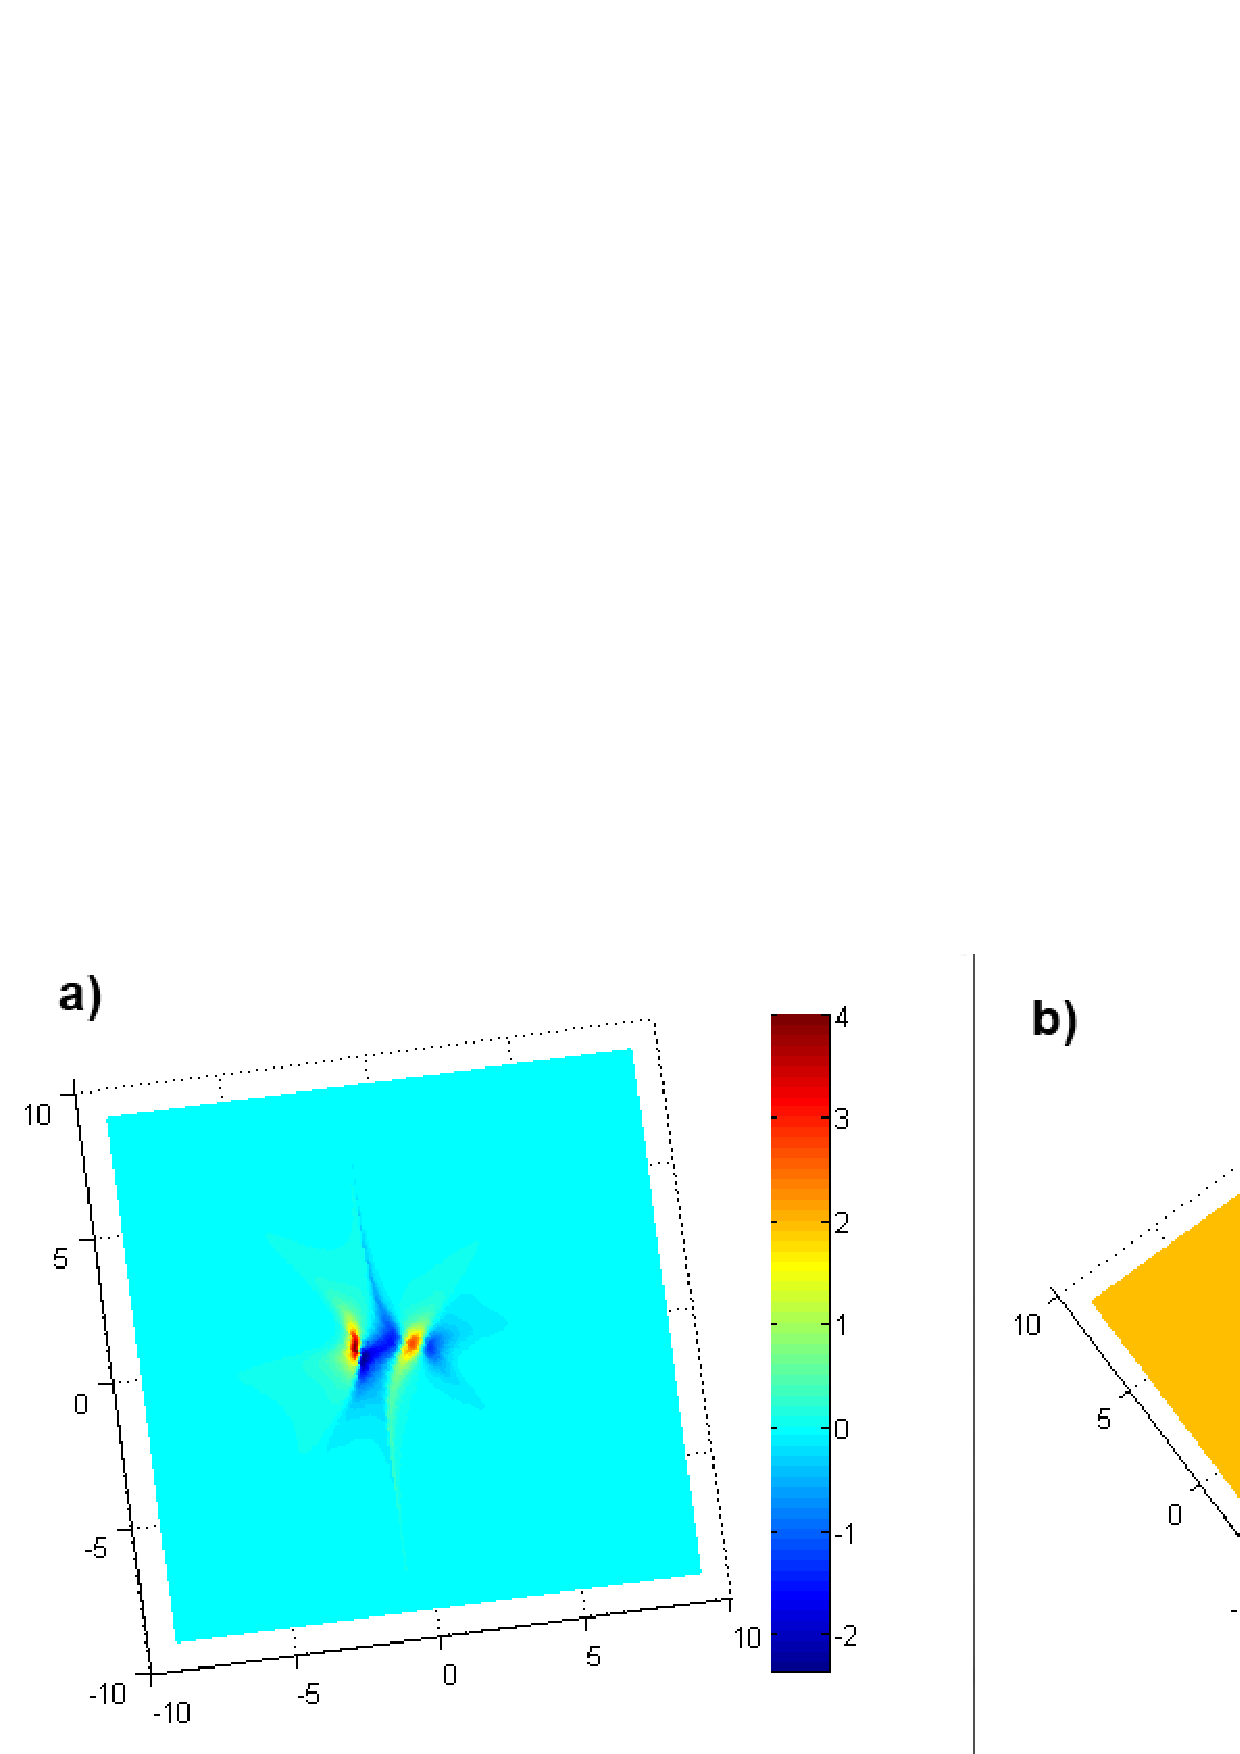
\includegraphics[width=150mm]{img/fmix_2d.png}
		\caption{2-Dimensional plots of both a) real and b) imaginary parts of nonlinear susceptibility treated as a bi-argumental function, where
		the colour means the function value \label{fig:fmix_2d}}
	\end{center}
\end{figure}

\begin{figure}
	\begin{center}
		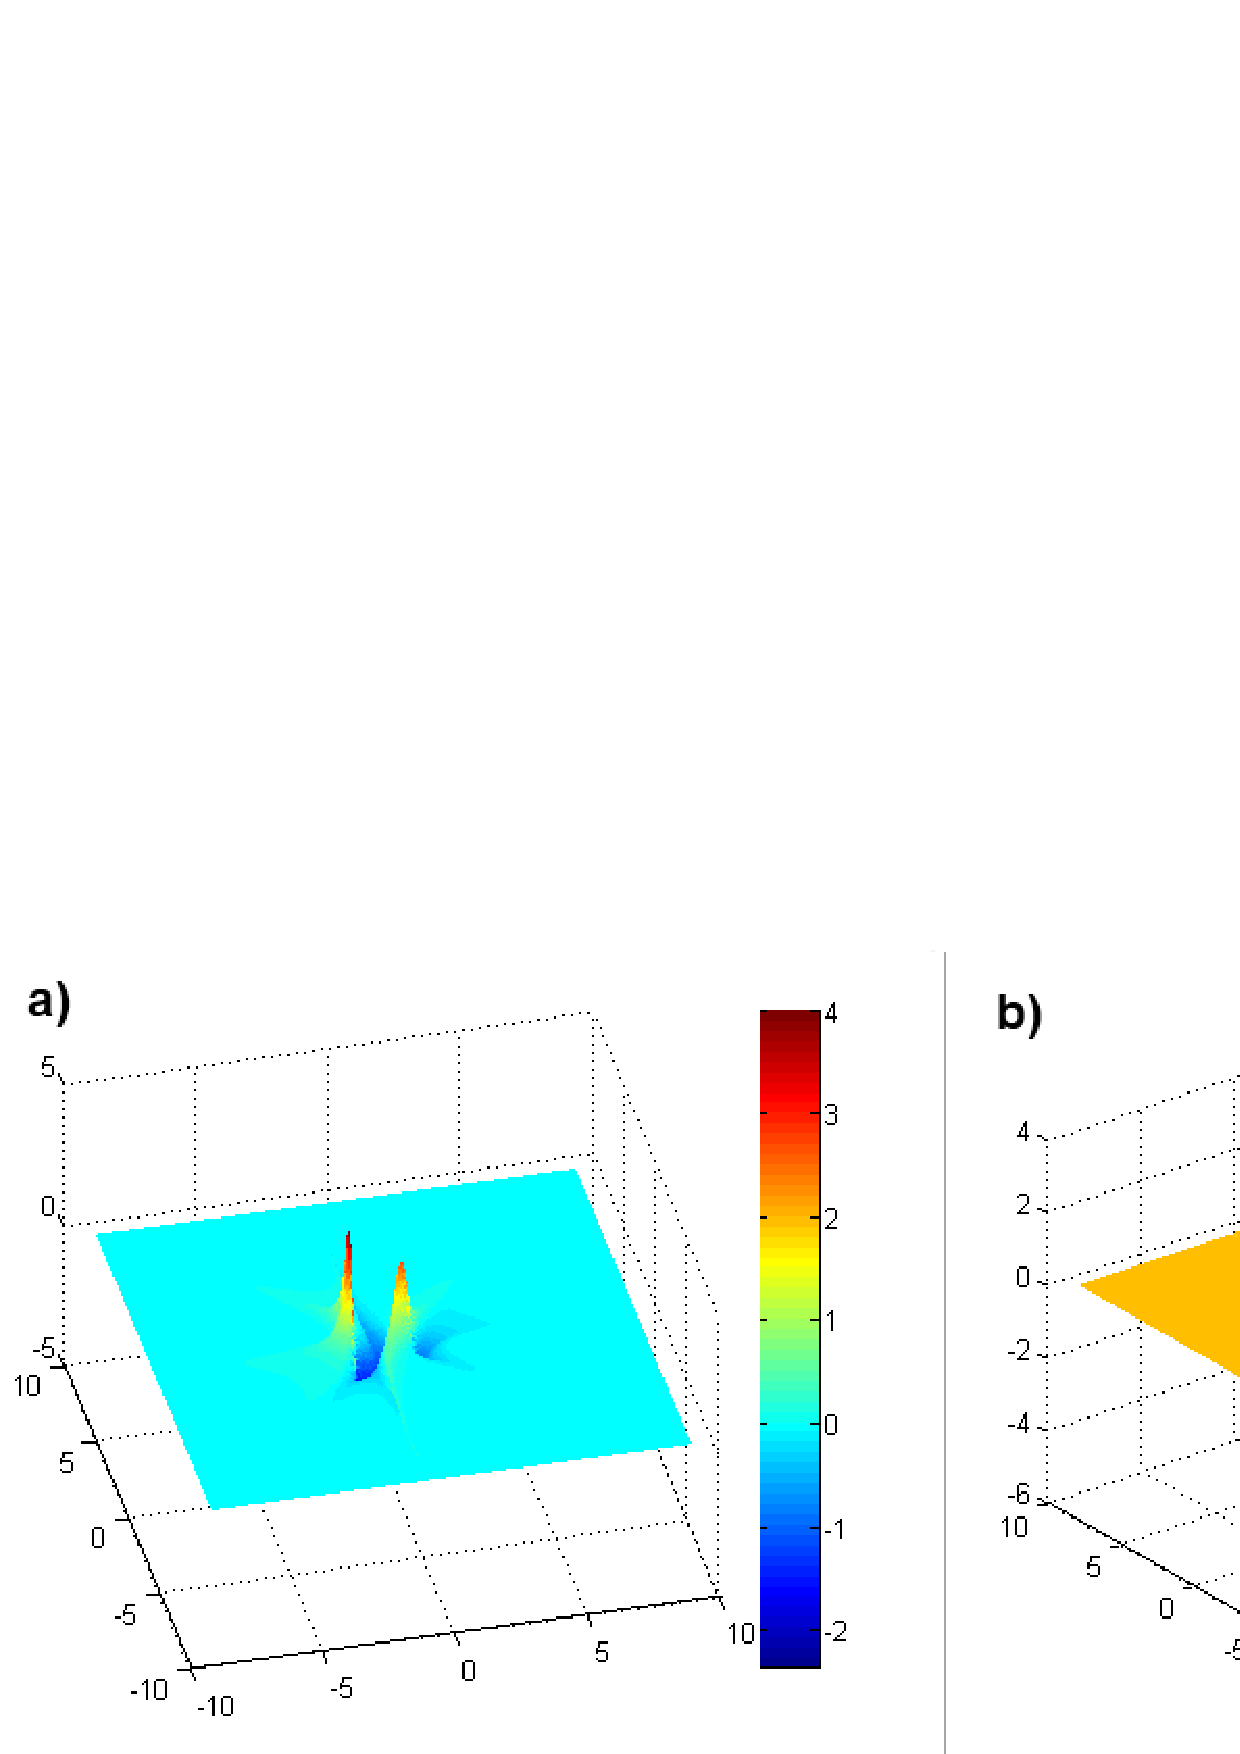
\includegraphics[width=150mm]{img/fmix_3d.png}
		\caption{3-Dimensional plots of both a) real and b) imaginary parts of nonlinear susceptibility treated as a bi-argumental function, where
		the colour means the function value \label{fig:fmix_3d}}
	\end{center} 
\end{figure}

We will shortly review the derivation of the Hilbert transform for nonlinear models. As proposed by Lucarini~\cite{lucarini_kramers}, we
connect the imaginary and the real part of the nonlinear optical susceptibility with the higher-level Hilbert transform:

\begin{subequations}  \label{eq:derivation_lucarini}
  \begin{multline} \label{eq:dlucarini_imag}
    \Im({\chi_{n, \,i, \,{j_1}, \,\ldots,\,{j_n}}}(\sum_{l=1}^{n}\,{\omega_l}, \,{\omega_1}, \,\ldots, \,{\omega_n})) =
    \\ \frac {-1}{( \pi )^{n}}  \dashint_{ - \infty }^{\infty }\,\ldots\,\dashint_{ - \infty
    }^{\infty }{ \frac { \Re({\chi_{n, \,i, \,{j_1}, \,\ldots, \,{j_n}}}(\sum_{l=1}^{n}\,{\Omega_l}, \,{\Omega_1}, \,
    \ldots, \,{\Omega_n}))}{({\Omega_1} - {\omega_1})\,\ldots\,({\Omega_n} - {\omega_n})} \,d{\Omega_1}\,\ldots\,d{\Omega_n}},
  \end{multline}
  \begin{multline} \label{eq:dlucarini_real}
    \Re({\chi_{n, \,i, \,{j_1}, \,\ldots, \,{j_n}}}(\sum_{l=1}^{n}\,{\omega_l}, \,{\omega_1},\,\ldots,\,{\omega_n})) = \\
    \frac {1}{\pi^{n}} \dashint_{ - \infty }^{\infty }\,\ldots\,\dashint_{ - \infty }^{\infty }
    \frac { \Im ({\chi_{n, \,i, \,{j_1}, \,\ldots, \,{j_n}}}(\sum_{l=1}^{n}\,{\Omega_l}, \,{\Omega_1}, \, \ldots,
    \,{\Omega_n}))}{({\Omega_1} - {\omega_1})\,\ldots\, ({\Omega_{n}} -
    {\omega_n})}\,d{\Omega_1}\,\ldots\,d{\Omega_n}.
  \end{multline}
\end{subequations}

These integrals are hard to solve numerically and they go beyond the subject of this thesis. Here we will assume a great simplification and
we will take only one frequency $\omega_{1}$ into consideration:

\begin{subequations}  \label{eq:derivation_conclude}
  \begin{multline}    \label{eq:dconclude_imag}
    \Im ({\chi_{n, \,i, \,{j_1}, \,\ldots, \,{j_n}}}(\sum_{l=1}^{n}\,{\omega_l}, \,{\omega_1}, \, \ldots, \,{\omega_n})) = \\
    \frac {-1}{\pi }  \dashint_{ - \infty }^{\infty }\frac {\Re ({\chi_{n, \,i, \,{j_{1}}, \, \ldots,
    \,{j_{n}}}}(\sum_{l=1}^{n}\,{\Omega_l}, \,{\Omega_1},  \,{\omega_2}, \, \ldots, \, {\omega_n}))}{{\Omega_1} - {
    \omega_1}}\,d{\Omega_1},
  \end{multline}
  \begin{multline}    \label{eq:dconclude_real}
    \Re ({\chi_{n, \,i, \,{j_{1}},  \, \ldots, \,{j_{n}}}}(\sum_{l=1}^{n}\,{\omega_l}, \,{\omega_1}, \, \ldots, \,{\omega_n})) = \\
    \frac {1}{\pi } \dashint_{ - \infty }^{\infty }\frac {\Im ({\chi_{n, \,i, \,{j_1}, \, \ldots,
    \,{j_{n}}}}(\sum_{l=1}^{n}\,{\Omega_l}, \,{\Omega_1}, \,{\omega_2}, \, \ldots, \,{\omega_n}))} {{\Omega_1} - {
    \omega_1}}\,d{\Omega_1}.
  \end{multline}
\end{subequations}

But we know that the signal response does not only depend on the input frequencies $\omega_{1},\dotsc,\omega_{n}$, but also on the time
delays between them $T_{1},\dotsc, ,T_{n-1}$:

\begin{equation} \label{eq:derive_withdelay}
   \chi_{n, \,i, \,j_{1},\dotsc,j_{n}} (\sum_{l=1}^{n}\,\omega_{l}, \,\omega_{1},\dotsc,
   \,\omega_{n}) = {\chi_{n, \,i, \,j_{1},\dotsc, \,j_{n} }}(\sum_{l=1}^{n}\,\omega_{l}, \,\omega_{1},\dotsc, 
   \, \omega_{n}, \,T_{1}, \dotsc, \,T_{N-1}).
 \end{equation}

Automatically we expand equation (\ref{eq:derivation_conclude}) into (\ref{eq:dcexpand_imag}) and (\ref{eq:dcexpand_real}):

\begin{subequations} \label{eq:dconlude_expand}
  \begin{multline}   \label{eq:dcexpand_imag}
    \Im ({\chi_{n, \,i, \,j_{1}, \,j_{2}, \, \ldots, \, j_{n}}} (\sum_{l=1}^{n}\,\omega_{l}, \, \omega_{1}, \,\omega_{2},
    \, \ldots, \,\omega_{n}, \,T_{1}, \,T_{2}, \, \ldots, \, T_{n - 1})) = \\
    \frac{-1}{ \pi } \dashint_{ - \infty }^{\infty } \frac {\Re
    ({\chi_{n, \,i, \,j_{1 }, \,j_{2}, \, \ldots, \,j_{n}}}(\sum_{l=1}^{n} \,\Omega_{l}, \, \Omega_{1}, \, \omega_{2}, \,\ldots,
    \, \omega_{n}, \,T_{1}, \,T_{2}, \,\ldots , \,T_{n - 1}))}{\Omega_{1} - \omega_{1}}\,d{\Omega_{1}}, 
  \end{multline}
  \begin{multline}   \label{eq:dcexpand_real}
    \Re ({\chi_{n, \,i, \,j_{1}, \,j_{2}, \, \ldots, \,j_{n}}}(\sum_{l=1}^{n}\,\omega_{l}, \,\omega_{1}, \, \omega_{2},
    \, \ldots, \, \omega_{n}, \,T_{1}, \, T_{2}, \, \ldots, \, T_{N - 1})) = \\
    \frac{1}{\pi } \dashint_{-\infty}^{\infty}\frac{\Im
    ({\chi_{n, \,i, \,j_{1 }, \,j_{2}, \, \ldots, \,j_{n}}}(\sum_{l=1}^{n} \,\Omega_{l}, \,\Omega_{1}, \,\omega_{2},
    \,  \ldots, \,\omega_{n}, \,T_{1}, \,T_{2}, \, \ldots, \, T_{n - 1}))}{\Omega_{1} - \omega_{1}} \,d{\Omega_{1}}.
  \end{multline}
\end{subequations}

The evaluation of the higher order Hilbert transforms will be a key to understand the mathematical model of the nonlinear optics. In this
thesis we make only a one little step forward.


\subsection{The quantum-perturbation models} \label{chap:problem_quantum}
The quantum mechanics is a part of physics where the microscopic particles and energies are described. We can call the quantum mechanics
also the quantum physics or the quantum theory. The main focus of the quantum physics is on the vectors describing the properties of
indicated physical system at a given time. These vectors are the sets of properties and physical values which are time and space
dependent. Such vectors are also named the complex wave functions. The values of such vectors are not unrestricted due to the main
assumption that any physical action must be a multiple of a small physical quantity - called the Planck constant: $h = 6.62606957(29) \times
10^{-34} \, \text{ Joule times second } $.

The maths used to describe the quantum world is far more complicated than one used in the classical physics and we will not get into the
details in this thesis. We will shortly introduce the two physical models of the quantum linear and nonlinear susceptibility described by
Kuzyk \cite{kuzyk_nlo} and Boyd \cite{boyd_nlo}. The calculations used in both cited works are based on the time-dependent perturbation.
The introduced concept of the perturbation is an interesting mathematical idea to solve difficult, differential equations.

\subsubsection*{The sum-over-states model}

The first model is named the sum-over-states. In this model we will sum all possible excited states and transitions between such states for
a single atom. In the linear case we assume that the atom can only be in $m$ excited states with no other option for atom than transition from
the ground state to one of the $m$ exited states and forth. The reason for such a prohibition is simple - we will assume only one photon is
interacting with the atom. You may associate the excited state with a situation when a single photon is absorbed by the atom and its energy
is added to the energy of the whole system.

In the nonlinear cases - we will assume that the number of possible atom states and inner-states transitions is increasing. To describe the
second-order nonlinear susceptibility we will assume there are $m$ possible troikas - so the combination of three possible states with an
option for transition between each state in a troika. To describe the third-order nonlinear susceptibility - we will assume that there
are $m$ possible fours of states.

We name this model the sum-over-states, because we will perform summation over all possible excited states for the theoretical model of an
atom. We have already introduced the Planck constant $h$. We will also used the $N$ constant to describe the number density of atoms - which
describe the concentration of any countable objects in a given, three-dimensional volume. We shall also introduce the vacuum permittivity constant
$\epsilon_0 \approx 8.854187817620 \times 10^{-12} \, \text{ Farad per meter } $. 

There are two more physical values to be discussed. First of the is $\mu_{i, ab}$ and the second is $\omega_{cd}$. $\mu_{i, ab}$ will be a
matrix-like value, and the $\omega_{cd}$ will be a vector-like value. There are many situations in physics, when a value is
described by the vector, two-dimensional matrix or a matrices of higher order. Such values are called \textbf{tensors}. $\mu_{ab}$ tensor
is described as the electric dipole moment with the Coulomb-meter SI unit. The electric dipole moment in physics describes the separation of
the negative and the positive charges in a systems consisting of charges. It is also called the system's polarity. It describes the polarity
of a system between a state ``a'' and the state ``b''. The order of indices also matters, so $\mu_{i, ab}$ is a different value from
$\mu_{i, ba}$. In our calculations this value will be a two-dimensional tensor - so a matrix - because one dimension will be related with
the ``ab'' or ``ba`` direction and the second dimension will be related with $i$ - the indicated spatial property of an atom. The atom
``shotted'' with a photon in the direction of the axis OX may behave different that ``shotted'' from the OY axis. This is also a
simplification and in general case the more photons are we taking into consideration, the higher order of a tensor need to be introduced.

The last value is an amount of energy related with a frequency $\omega_{cd}$ required for an atom to make a transition between state
``c'' and state ``d''. We will use a one-dimensional tensor to describe this value. $P_{I}$ is the intrinsic permutation operator, in
general it is used not to repeat the very same summands again and again just with slight modification of $+$ and $-$ signs - but please see
details in \cite{boyd_nlo}.

The $\omega_{p}$ is the frequency of the input photon and it will be a variable in our equations. The final equations are taken from Boyd
\cite{boyd_nlo}. They describe the linear (first order) optical susceptibility and the nonlinear (second and third order) optical
susceptibilities as a functions of $\omega_{p}$:


% Quantum-perturbation - result model equation - linear case
\begin{equation} \label{eq:sresults_linear}   
  { \chi_{1, \, i, \, j } } ( {\omega_{p} } ) = \frac {N} { {\varepsilon_{0} } \, h} 
    \sum_{m} \, 
      ( \frac { {\mu_{i, \, gm} } \, {\mu_{j, \, mg} } } { {\omega_{mg} } - {\omega_{p} } } 
      + \frac { {\mu_{j, \, gm} } \, {\mu_{i, \, mg} } } { {\omega_{mg} } + {\omega_{p} } } ),
\end{equation}

% Quantum-perturbation - result model equation - second-order case
\begin{equation} \label{eq:sresults_quadratical}
  \begin{split}
    & \chi_{2, \, i, \, j, \, k}({\omega_{p}} + {\omega_{q}}, \, {\omega_{q}}, \, {\omega_{p}}) = 
        \frac{N}{{\varepsilon_{0}}\,h^{2}}{P_{I}}\, \sum_{mn}\, 
 \\ & ( \frac{{\mu_{i, \, gn}} \, {\mu_{j,\,nm}} \, {\mu_{k, \, mg}}}
             {(\omega_{ng} - \omega_{p} - {\omega_{q}})\,({ \omega_{mg}} - {\omega_{p}})} 
 \\ & + \frac{{\mu_{j, \, gn}} \, {\mu_{i,\,nm}} \, {\mu_{k, \, mg}}}
             {(\omega_{ng} + \omega_{q})\,(\omega_{mg} - \omega_{p})}
 \\ & + \frac{{\mu_{i, \, gn}} \, {\mu_{k,\,nm}} \, {\mu_{i, \, mg}}}
             {(\omega_{ng} + \omega_{q})\,(\omega_{mg} + \omega_{p}+ \omega_{q})})
  \end{split} 
\end{equation}

% Quantum-perturbation - result model equation - third-order case
\begin{equation} \label{eq:sresults_cubic}
  \begin{split}
    & \chi_{3, \,k, \,j, \,i, \,h} ({\omega_{\sigma }}, \,{\omega_{r}}, \,{\omega_{q}}, \,{\omega_{p}}) 
      = \frac{N}{{\varepsilon_{0}} \, h^{3}} {P_{I}} \! \sum_{mnv}\,
 \\ & ( \frac {{\mu_{k, \,gv}} \, {\mu_{j, \,vn}} \, {\mu_{i,\,nm}} \, {\mu_{h, \,mg}}} 
              {({\omega_{vg}} - {\omega_{r}} - {\omega_{q}} - {\omega_{p}})\,
               ({\omega_{ng}} - {\omega_{q}} - {\omega_{p}}) \,
               ({\omega_{mg}} - {\omega_{p}})} 
 \\ & + \frac {{\mu_{j, \,gv}} \, {\mu_{k, \,vn}} \, {\mu_{i, \,nm}} \, {\mu_{h, \,mg}}}
              {({\omega_{vg}} + {\omega_{r}}) \,
               ({\omega_{ng}} - {\omega_{q}} - {\omega_{p}}) \,
               ({\omega_{ mg}} - {\omega_{p}})} 
 \\ & + \frac {{\mu_{j, \,gv}} \, {\mu_{i, \,vn}} \, {\mu_{k, \,nm}} \, {\mu_{h, \,mg}}}
              {({\omega_{vg}} + {\omega_{r}}) \,
               ({\omega_{ng}} + {\omega_{r}} + {\omega_{q}}) \,
               ({\omega_{mg}} - {\omega_{p}})} 
 \\ & + \frac {{\mu_{j, \,gv}} \, {\mu_{i, \,vn}} \, {\mu_{h,\,nm}} \, {\mu_{k, \,mg}}}
              {({\omega_{vg}} + {\omega_{r}}) \, 
               ({\omega_{ng}} + {\omega_{r}} + {\omega_{q}} ) \, 
               ({\omega_{mg}} + {\omega_{r}} + {\omega_{q}} + { \omega_{p}})}).
  \end{split}
\end{equation}

\subsubsection*{The density matrix model}

Starting from the models described in the (\ref{eq:sresults_linear}), (\ref{eq:sresults_quadratical}) and (\ref{eq:sresults_cubic})
equations we can easily jump to the density matrix operator models. Not getting into the theoretical background - we will introduce a new
term $\gamma_{ab}$ which will be the imaginary tensor describing the so called dumping rate, which is an element of the density matrix,
describing the coherence between states $a$ and $b$. The models have been described in the following equations:

% Quantum-perturbation density matrix - result model equation - linear case
\begin{equation} \label{eq:ssmods_linear}
    {\chi_{1}}({\omega_{p}}) = \frac {N}{{\varepsilon_{0}}\,h}\sum_{n}\,(\frac {{\mu_{i, \,an}}\,{\mu_{j, \,na}}}{{\omega_{na}} -
    {\omega_{p}} - i\,{\gamma_{na}}} + \frac {{\mu_{i, \,na}}\,{\mu_{j, \,an}}}{{\omega_{na}} - {\omega_{p}} + i\,{\gamma_{na}}}),
\end{equation}

% Quantum-perturbation density matrix - result model equation - second-order case
\begin{equation} \label{eq:ssmods_quadratical}
  \begin{split}
    & {\chi_{2, \,i, \,j, \,k}}({\omega_{p}} + {\omega_{q}}, \,{\omega_{q}}, \,{\omega_{p}}) 
      = \frac{N} {2 \, {\varepsilon_0} \, h^{2}} 
        \sum_{lmn} \, {\rho_{0, \,ll}} \, 
 \\ & ( \frac {{\mu_{i, \,l, \,n}} \, {\mu_{j, \,nm}} \, {\mu_{k, \,ml}}} 
              {({\omega_{nl}} - {\omega_{p}} - {\omega_{q}} - i\,{\gamma_{nl}}) \,
               ({\omega_{ml}} - {\omega_{p}} - i\,{\gamma_{ml}}) } 
 \\ & + \frac {{\mu_{i, \,l, \,n}}\,{\mu_{k, \,nm}}\,{\mu_{j, \,ml}}}
              {({\omega_{nl}} - {\omega_{p}} - {\omega_{p}} - i\,{\gamma_{nl}}) \,
               ({\omega_{ml}} - {\omega_{q}} - i\,{\gamma_{ml}})} 
 \\ & + \frac {{\mu_{k, \,l, \,n}}\,{\mu_{i, \,nm}}\,{\mu_{j,\,ml}}}
              {({\omega_{mn}} - {\omega_{p}} - {\omega_{q}} - i\,{\gamma_{mn}}) \,
               ({\omega_{nl}} + {\omega_{q}} + i\,{\gamma_{nl}})}
 \\ & + \frac {{\mu_{j, \,l, \,n}}\,{\mu_{i, \,nm}}\,{\mu_{k, \,ml}}}
              {({\omega_{mn}} - {\omega_{p}} - {\omega_{q}} - i\,{\gamma_{mn}}) \,
               ({\omega_{nl}} + {\omega_{q}} + i\,{\gamma_{nl}})}
 \\ & + \frac {{\mu_{j, \,l, \,n}}\,{\mu_{i, \,nm}}\,{\mu_{k,\,ml}}}
              {({\omega_{nm}} + {\omega_{p}} + {\omega_{q}} + i\,{\gamma_{nm}}) \,
               ({\omega_{ml}} - {\omega_{p}} - i\,{\gamma_{ml}})}
 \\ & + \frac {{\mu_{k, \,l, \,n}}\,{\mu_{j, \,nm}}\,{\mu_{i, \,ml}}}
              {({\omega_{nm}} + {\omega_{p}} + {\omega_{q}} + i\,{\gamma_{nm}}) \,
               ({\omega_{ml}} - {\omega_{p}} - i\,{\gamma_{ml}})} 
 \\ & + \frac {{\mu_{k, \,l, \,n}}\,{\mu_{j, \,nm}}\,{\mu_{i, \,ml}}}
              {({\omega_{ml}} + {\omega_{p}} + {\omega_{q}} + i\,{\gamma_{ml}}) \,
               ({\omega_{nl}} + {\omega_{p}} + i\,{\gamma_{nl}})}
 \\ & + \frac {{\mu_{j, \,l, \,n}}\,{\mu_{k, \,nm}}\,{\mu_{i, \,ml}}}
              {({\omega_{ml}} + {\omega_{p}} + {\omega_{q}} + i\,{\gamma_{ml}}) \,
               ({\omega_{nl}} + {\omega_{q}} + i\,{\gamma_{nl}})} ),
  \end{split}
\end{equation}

% Quantum-perturbation density matrix - result model equation - third-order case
\begin{equation} \label{eq:ssmods_cubic}
  \begin{split}
    & {\chi_{3, \,k, \,j, \,i, \,h}}({\omega_{p}} + {\omega_{q}} + {\omega_{r}}, \,{\omega_{r}}, \,{\omega_{q}}, \,{\omega_{p}})
       = \frac {N} {{\varepsilon_{0}}\,h^{3}} \, \cdot \, \sum_{vnml}\,{\rho_{0, \,ll}} \, 
 \\ & ( \frac {{\mu_{k,\,lv}}\,{\mu_{j,\,vn}}\,{\mu_{i,\,nm}}\,{\mu_{h,\,ml}}}
  	          {({\omega_{vl}} - {\omega_{p}} - {\omega_{q}} - {\omega_{r}} - i\,{\gamma_{vl}}) \,
  	           ({\omega_{nl}} - {\omega_{p}} - {\omega_{q}} - i\,{\gamma_{nl}}) \,
  	           ({\omega_{ml}} - {\omega_{p}} - i\,{\gamma_{ml}})} 
 \\ & + \frac {{\mu_{h,\,lv}}\,{\mu_{k,\,vn}}\,{\mu_{j,\,nm}}\,{\mu_{i,\,ml}}}
              {({\omega_{nv}} - {\omega_{p}} - {\omega_{q}} - {\omega_{r}} - i\,nv) \,
               ({\omega_{mv}} - {\omega_{p}} - {\omega_{q}} - i\,{\gamma_{mv}}) \,
               ({\omega_{vl}} + {\omega_{p}} + i\,{\gamma_{vl}})}
 \\ & + \frac {{\mu_{i,\,lv}}\,{\mu_{k,\,vn}}\,{\mu_{j,\,nm}}\,{\mu_{h,\,ml}}}
              {({\omega_{nv}} - {\omega_{p}} - {\omega_{q}} - {\omega_{r}} - i\,{\gamma_{nv}}) \,
               ({\omega_{vm}} + {\omega_{p}} + {\omega_{q}} + i\,{\gamma_{vm}}) \,
               ({\omega_{ml}} - {\omega_{p}} - i\,{\gamma_{ml}})}
 \\ & + \frac {{\mu_{h,\,lv}}\,{\mu_{i,\,vn}}\,{\mu_{k,\,nm}}\,{\mu_{j,\,ml}}}
              {({\omega_{mn}} - {\omega_{p}} - {\omega_{q}} - {\omega_{r}} - i\,{\gamma_{mn}}) \,
               ({\omega_{nl}} - {\omega_{p}} - {\omega_{q}} + i\,{\gamma_{nl}}) \,
               ({\omega_{vl}} + {\omega_{p}} + i\,{\gamma_{vl}})} 
 \\ & + \frac {{\mu_{j,\,lv}}\,{\mu_{k,\,vn}}\,{\mu_{i,\,nm}}\,{\mu_{h,\,ml}}}
              {({\omega_{vn}} - {\omega_{p}} - {\omega_{q}} - {\omega_{r}} + i\,{\gamma_{vn}}) \,
               ({\omega_{nl}} - {\omega_{p}} - {\omega_{q}} - i\,{\gamma_{nl}}) \,
               ({\omega_{ml}} - {\omega_{p}} - i\,{\gamma_{ml}})}
 \\ & + \frac {{\mu_{h,\,lv}}\,{\mu_{j,\,vn}}\,{\mu_{k,\,nm}}\,{\mu_{i,\,ml}}}
              {({\omega_{nm}} + {\omega_{p}} + {\omega_{q}} + {\omega_{r}} + i\,{\gamma_{nm}}) \,
               ({\omega_{mv}} - {\omega_{p}} - {\omega_{q}} - i\,{\gamma_{mv}}) \,
               ({\omega_{vl}} + {\omega_{p}} + i\,{\gamma_{vl}})}
 \\ & + \frac {{\mu_{i,\,lv}}\,{\mu_{j,\,vn}}\,{\mu_{k,\,nm}}\,{\mu_{h,\,ml}}}
              {({\omega_{vm}} + {\omega_{p}} + {\omega_{q}} + {\omega_{r}} + i\,{\gamma_{nm}}) \,
               ({\omega_{vm}} + {\omega_{p}} + {\omega_{q}} + i\,{\gamma_{mv}}) \,
               ({\omega_{ml}} - {\omega_{p}} - i\,{\gamma_{ml}})} 
 \\ & + \frac {{\mu_{h, \,lv}}\,{\mu_{i,\,vn}}\,{\mu_{j,\,mn}}\,{\mu_{k,\,ml}}}
              {({\omega_{ml}} + {\omega_{p}} + {\omega_{q}} + {\omega_{r}} + i\,{\gamma_{ml}}) \,
               ({\omega_{nl}} + {\omega_{p}} + {\omega_{q}} + i\,{\gamma_{nl}}) \,
               ({\omega_{vl}} + {\omega_{p}} + i\,{\gamma_{vl}})}).
  \end{split}
\end{equation}


What is interesting, after expanding all the permutations in (\ref{eq:ssmods_cubic}) we will get the 48 different
summands - which show how the quantum mechanical approach is hard to apply.

In further calculations we will use both the presented equations in simplified version - with just a few summands. The visualization of the
results for a typical quantum-perturbative model obtained with equation (\ref{eq:ssmods_cubic}) are shown in Figure (\ref{fig:qp_plot}).

\begin{figure}
	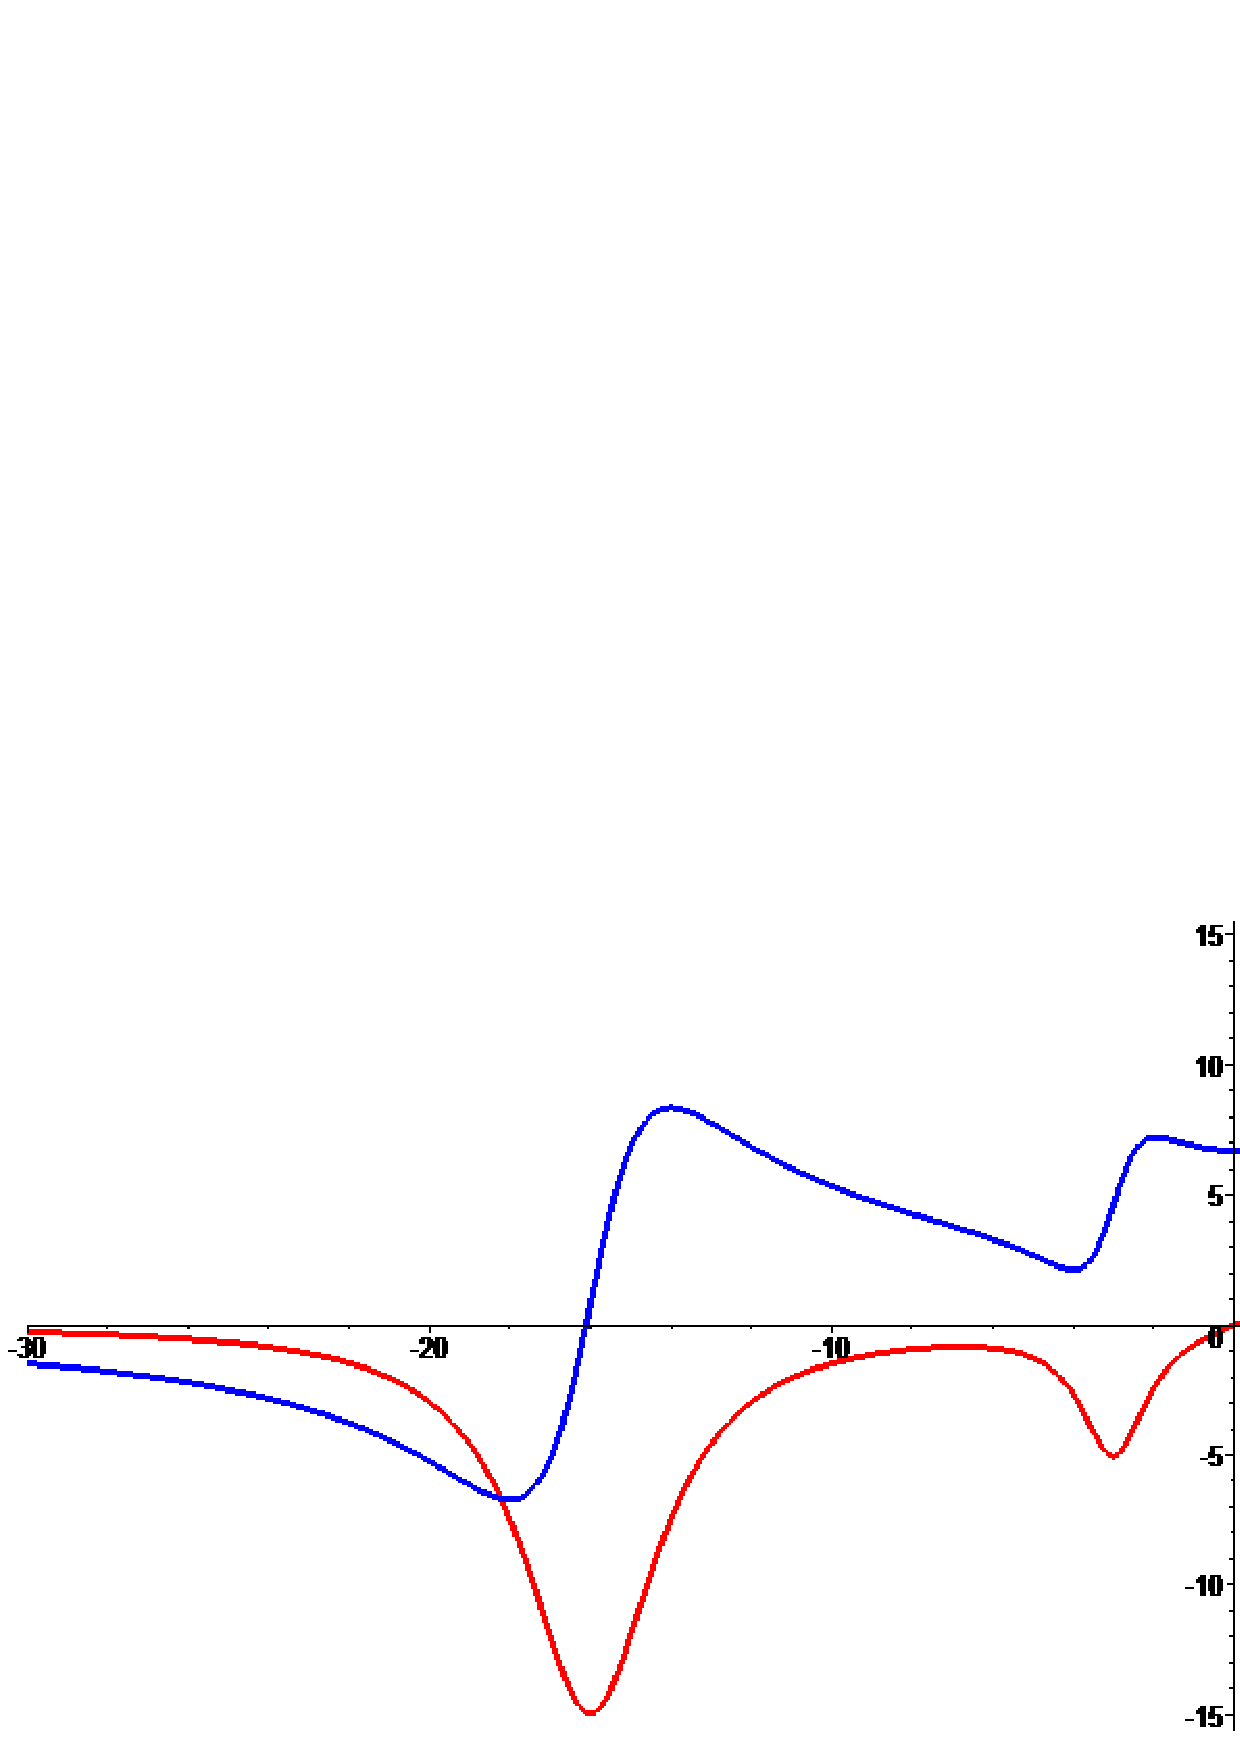
\includegraphics[width=150mm]{img/qp_plot.png}
	\caption{Quantum-perturbative plot for 3-level model of with arbitrary (non-physical) parameters. Red plot is for the imaginary and the
	blue plot is for the real part of the linear susceptibility. \label{fig:qp_plot}}
\end{figure}

\begin{figure} 
  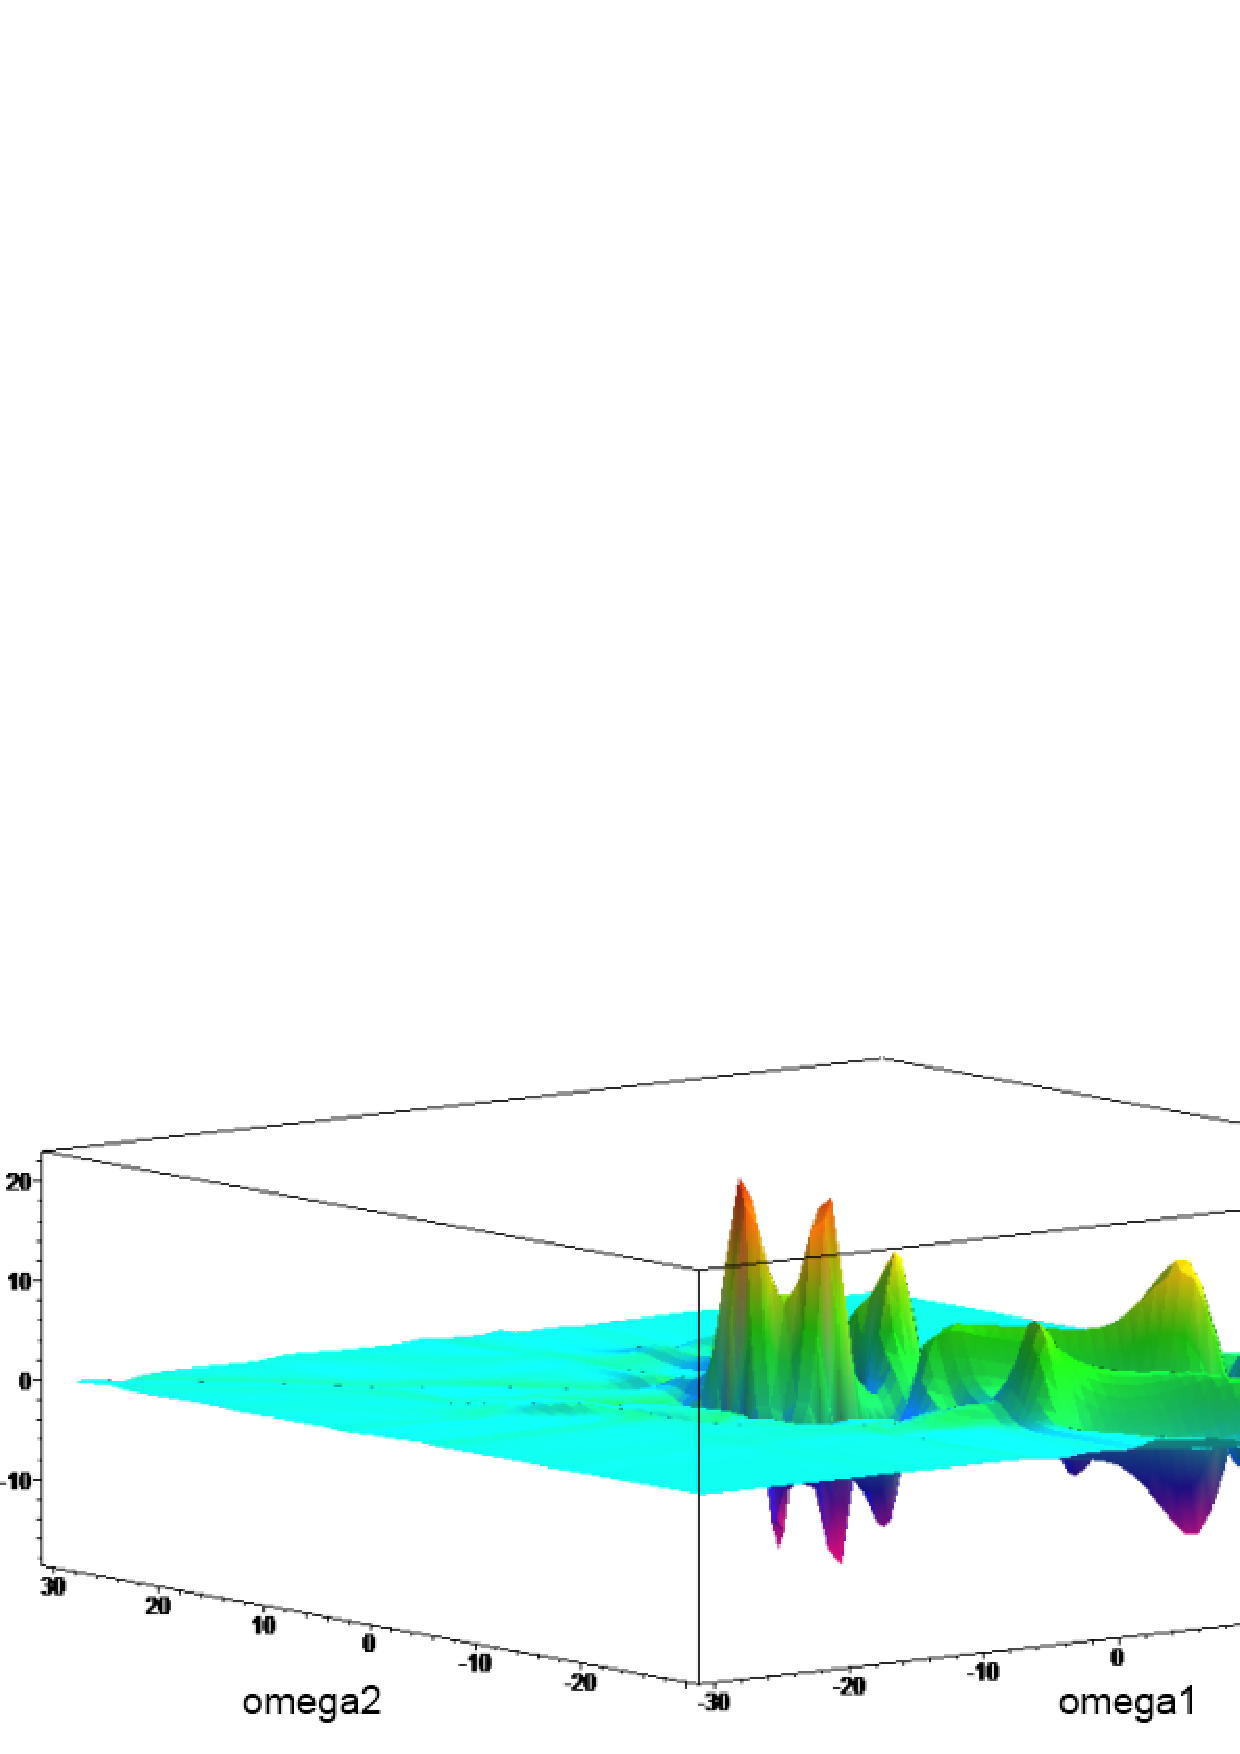
\includegraphics[width=150mm]{img/qp_3da.png} \\
  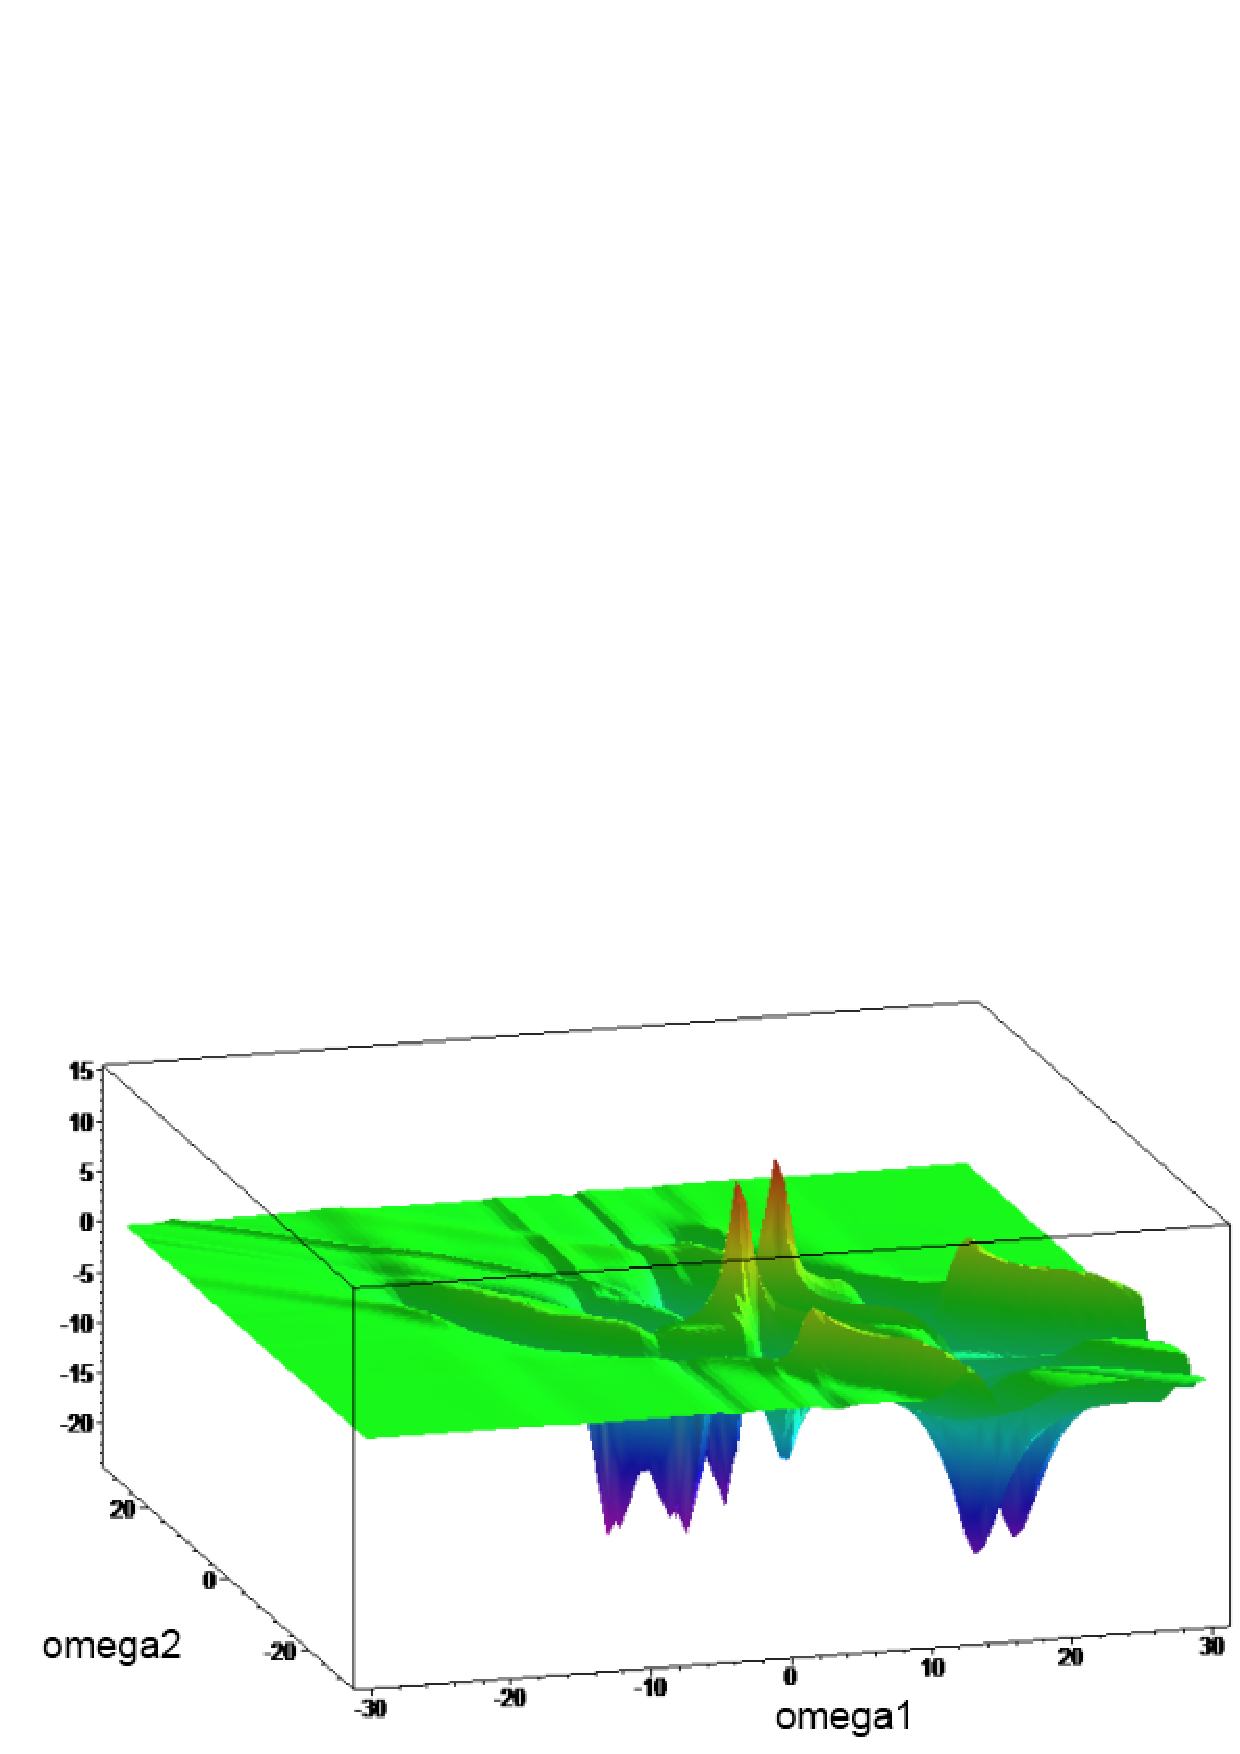
\includegraphics[width=150mm]{img/qp_3db.png}
  \caption{Three dimensional quantum-perturbative plot for 3-level model of with arbitrary (non-physical) parameters. Upper plot is for the
  imaginary and the lower plot is for the real part of the second-order susceptibility.
  \label{fig:qp_3d}}
\end{figure}
   
\section{Simpson and trapezoidal quadrature based Hilbert transform - HTRAN} \label{chap:htran}

\subsection{Overview of the HTRAN} \label{chap:htran_overview}

In this chapter we present the simplest possible but still nice working numerical calculation of the Hilbert transform based on the report
by I. J. Weinberg \cite{weinberg_hilbert}. It uses the Simpson and trapezoidal quadrature. We have slightly modified author's algorithm and
it no longer requires the input to be an even function.

The algorithm is presented in two parts. In the first part, we present how the Hilbert transform equation can be modified with one strict
assumption from the singular integral to the non-singular one. In the second part, we will use the new set of input function
values based on the interpolation method.

\begin{figure}
	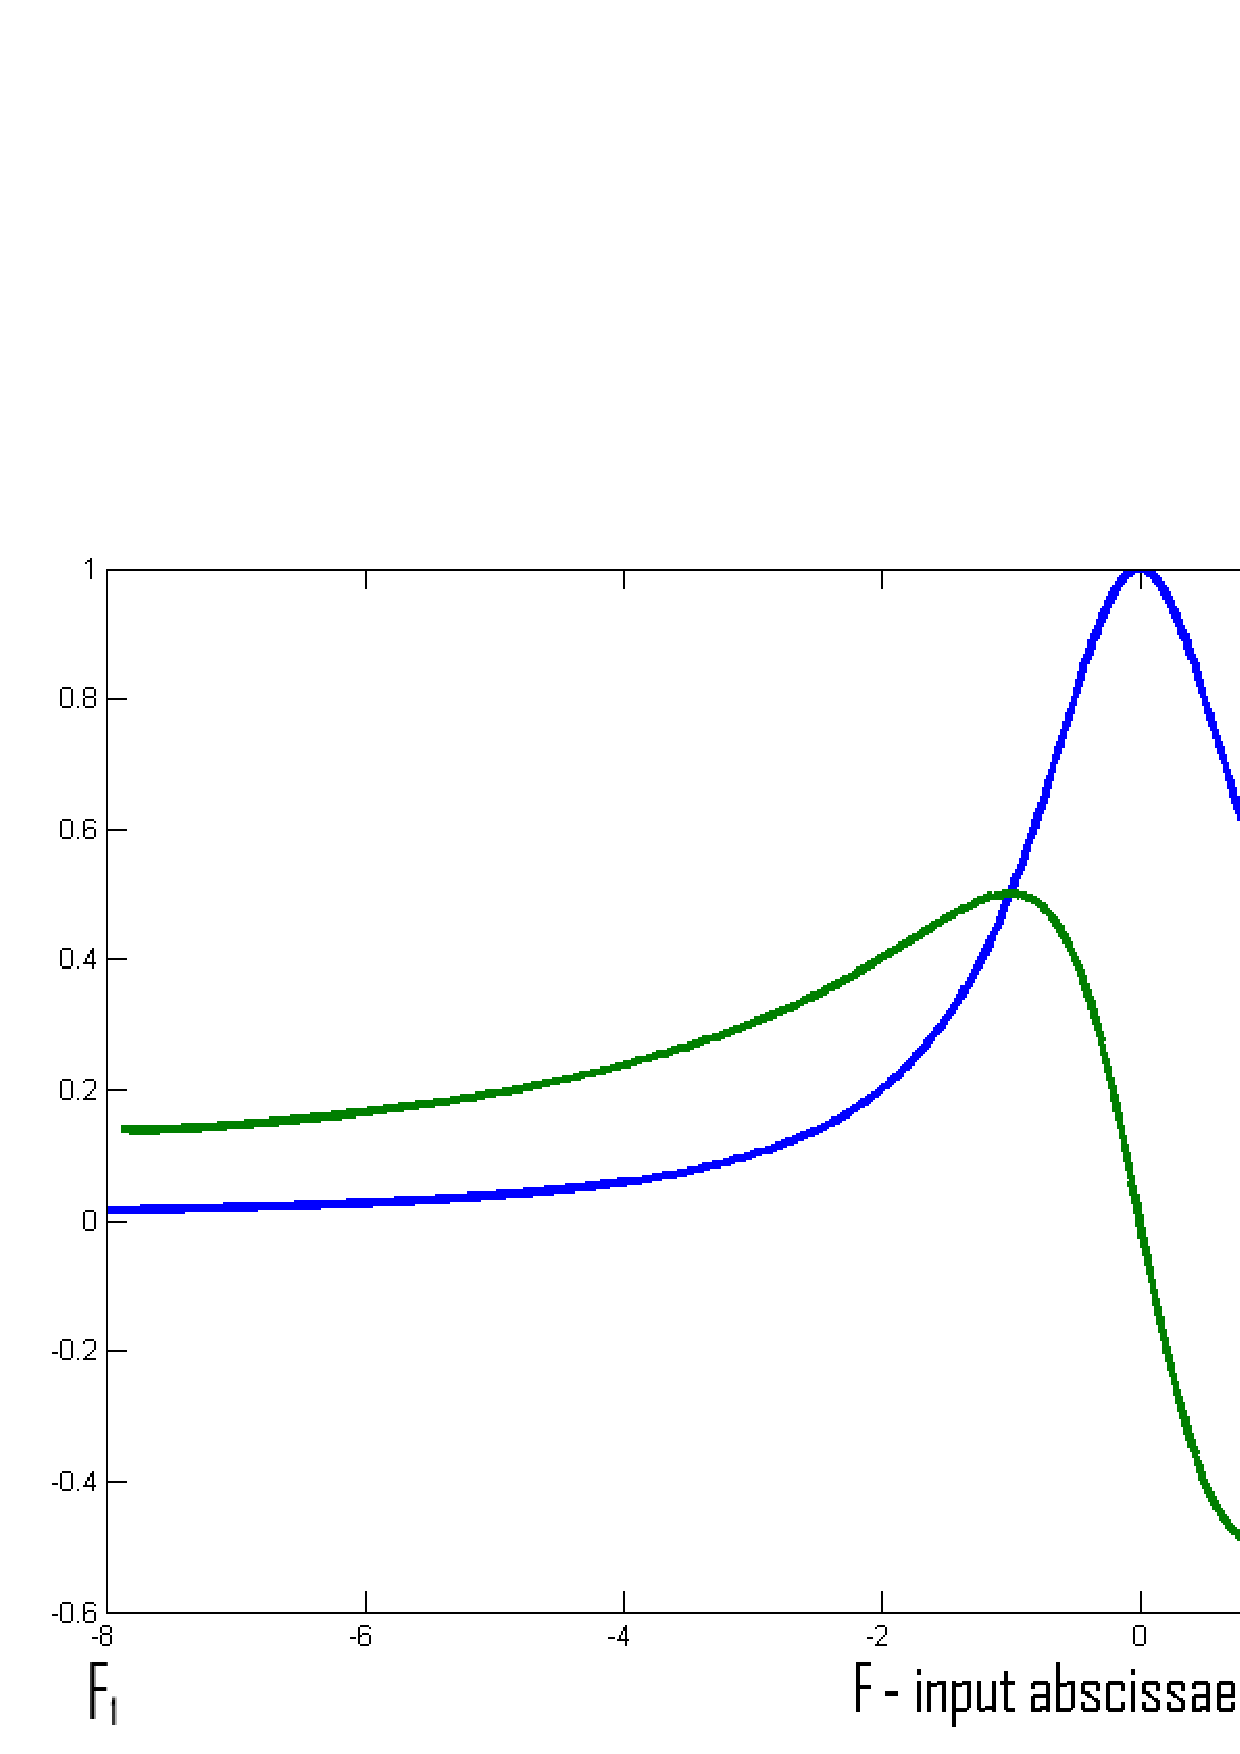
\includegraphics[width=150mm]{img/htran_illustration.png}
	\caption{A sample input plot (ordered pairs of OX abscissae - F - and the OY ordinates - R) with the sample output plot HT for the HTRAN
	algorithm. \label{fig:htran_illustration}} 
\end{figure}

We assume that the input function R is defined for a discrete set of arguments:
 
\begin{equation} \label{eq:htran_arguments}
	F = \{ F_1, F_2, \ldots, F_N \} \quad (F_i < F_j \, \text{ for } i < j) . 
\end{equation}

We will calculate the Hilbert transform of $R$ for the same discrete set of arguments $F$. An example has been presented on Figure
(\ref{fig:htran_illustration}), where the blue plot represents the input function $R$ and the green plot represents the output function $HT$.


We start from reminding the definition of the Hilbert transform:

\begin{equation} \label{eq:htran_basic_representation}
 \mathrm{HT}(\omega )
  = \frac{1}{\pi } {\dashint_{ - \infty }^{\infty }  \frac {\mathrm{R}(\Omega )}{\Omega - \omega }\,d\Omega }
\end{equation}

We transform the basic representation (\ref{eq:htran_basic_representation}) into a limit of two integrals:

\begin{equation} \label{eq:htran_first_modification}
  \frac{1}{\pi } {\dashint_{ - \infty }^{\infty }  \frac {\mathrm{R}(\Omega )}{\Omega - \omega }\,d\Omega }
  = {\lim_{\varepsilon \rightarrow 0}} 
  	\left( \int_{ - \infty }^{\omega - \varepsilon } \frac {\mathrm{R}(\Omega )}{\Omega - \omega }\,d\Omega  
  	     + \int_{ \omega + \varepsilon }^{ \infty  } \frac {\mathrm{R}(\Omega )}{\Omega - \omega }\,d\Omega \right) .
\end{equation} 

Now for each frequency $\omega$ we observe the following property:

\begin{equation} \label{eq:htran_cpv_property}
	\dashint_{ - \infty }^{\infty } \frac {1}{\Omega  - \omega } \,d\Omega =0 .
\end{equation}

We use the observation (\ref{eq:htran_cpv_property}) and modify the equation (\ref{eq:htran_first_modification}):

\begin{equation} \label{eq:htran_newintegral}
  \mathrm{HT}(\omega )
  = \frac{1}{\pi } {\dashint_{ - \infty }^{\infty } \frac {\mathrm{R}(\Omega ) - \mathrm{R}(\omega )}{\Omega  - \omega }\,d\Omega }
  + \frac{1}{\pi } {\dashint_{ - \infty }^{\infty } \frac {\mathrm{R}(\Omega )}{\Omega  - \omega }\,d\Omega }
  = \frac{1}{\pi } {\dashint_{ - \infty }^{\infty } \frac {\mathrm{R}(\Omega ) - \mathrm{R}(\omega )}{\Omega - \omega }\,d\Omega} . 
\end{equation}

We can easily transform the result of the (\ref{eq:htran_newintegral}) as follows:

\begin{equation} \label{eq:htran_ht_three}
  \mathrm{HT}(\omega ) = \frac{1}{\pi } \left[ 
    \int_{ -\infty }^{F_1} \frac {\mathrm{R}(\Omega ) - \mathrm{R}(\omega )}{\Omega  - \omega }\,d\Omega 
  + \int_{ F_1 }^{ F_N }   \frac {\mathrm{R}(\Omega ) - \mathrm{R}(\omega )}{\Omega  - \omega }\,d\Omega 
  + \int_{ F_N }^{ \infty} \frac {\mathrm{R}(\Omega ) - \mathrm{R}(\omega )}{\Omega  - \omega }\,d\Omega 
  \right] .
\end{equation}

As the input function R is assumed to be square-integrable, we will put even more strict assumption:

\begin{equation} \label{eq:htran_vanishes}
  \mathrm{R}(\omega) = 0 \, \text{ for } \omega < F_1 \, \text { or } \, \omega > F_N.  
\end{equation}

With the strict-vanishing assumption (\ref{eq:htran_vanishes}) for $R(\omega)$, we can simplify the equation (\ref{eq:htran_ht_three}) as
follows:

\begin{equation} \label{eq:htran_ht}
  \mathrm{HT}(\omega ) = \frac{1}{\pi } \left[ 
    \int_{ -\infty }^{F_1} - \frac {\mathrm{R}(\omega )}{\Omega - \omega }\,d\Omega
  + \int_{ F_1 }^{ F_N }     \frac {\mathrm{R}(\Omega ) - \mathrm{R}(\omega )}{\Omega - \omega }\,d\Omega 
  + \int_{ F_N }^{ \infty} - \frac {\mathrm{R}(\omega )}{\Omega - \omega }\,d\Omega 
  \right] .
\end{equation}

As $\omega  \in [F_1, \,F_N]$  we will now consider two cases - that takes into account the position of  $\omega $ in relation to $F_1$  and
$F_N$ We have two possibilities:

\begin{equation}   \label{eq:htran_twoposibilities}
	\omega - F_1 < F_N - \omega \, \text{ and } F_N - \omega \leq \omega - F_1 
\end{equation}

We shall also notice the symmetry property of the the function $\frac {1}{\Omega - \omega }$ for any $M > 0$:

\begin{equation} \label{eq:htran_forallm}
    \int_{ -\infty}^{\omega - M}\frac {1}{\Omega - \omega}\,d\Omega 
  + \int_{\omega + M}^{ \infty }\frac {1}{\Omega - \omega}\,d\Omega = 0
\end{equation}

Together with the observation (\ref{eq:htran_forallm}) each of two cases from (\ref{eq:htran_twoposibilities}) leads to results obtained
in equations (\ref{eq:htran_htres1}) and (\ref{eq:htran_htres2}) respectively:

\begin{subequations} \label{eq:htran_htresults}
  \begin{multline}   \label{eq:htran_htres1}
    \mathrm{HT}(\omega )= \frac {1}{\pi} 
    \left[
        \int_{2\,\omega - F_N}^{F_1} - \frac {\mathrm{R}(\omega )}{\Omega - \omega }\,d\Omega 
      + \int_{F_1}^{F_N} \frac {\mathrm{R}(\Omega ) - \mathrm{R}(\omega )}{\Omega - \omega }\,d\Omega 
    \right] \\
    = \frac {1}{\pi} 
    \left[ 
      - \mathrm{R}(\omega )\,\mathrm{ln}(\frac {F_1 - \omega }{\omega - F_N}) 
      + \int_{F_1}^{F_N}\frac {\mathrm{R}( \Omega ) - \mathrm{R}(\omega )}{\Omega  - \omega }\,d\Omega  
    \right] ,
  \end{multline}
  \begin{multline}   \label{eq:htran_htres2}
    \mathrm{HT}(\omega ) = \frac {1}{\pi} 
    \left[
        \int_{F_1}^{F_N}\frac {\mathrm{R}(\Omega )- \mathrm{R}(\omega)}{\Omega - \omega }\,d\Omega 
      + \int_{F_N}^{2\,\omega - F_1}\frac { - \mathrm{R}(\omega )}{\Omega  - \omega }\,d\Omega
    \right] \\
    = \frac {1}{\pi} 
    \left[ 
        \int_{F_1}^{F_N}\frac {\mathrm{R}(\Omega ) - \mathrm{R}(\omega )}{\Omega  - \omega }\,d\Omega 
      - \mathrm{R}( \omega )\,\mathrm{ln}(\frac {\omega - F_1}{F_N - \omega })
    \right] .
  \end{multline}
\end{subequations}

And we can see that both the (\ref{eq:htran_htresults}) derivations lead to the same result:

\begin{equation} \label{eq:htran_sameresult}
  \mathrm{HT}(\omega ) = \frac {1}{\pi } 
  \left[
      - \mathrm{R}(\omega )\, \mathrm{ln}( \frac {\omega  - F_1}{F_N - \omega }) 
      + \int_{F_1}^{ F_N}\frac {\mathrm{R}(\Omega ) - \mathrm{R}(\omega )}{\Omega - \omega }\,d\Omega
  \right] 
\end{equation}

We also observe that for any $\omega$ inside the range $[F_1, \,F_N] $ both values $\omega  - F_1$ and $F_N - \omega$ are non-negative.
That leads to a simple observation that condition $0 < \frac {\omega - F_1}{F_N - \omega }$ is satisfied and therefore the logarithm
argument is well defined. What now interests us the most, is the integral:

\begin{equation} \label{eq:htran_interestint} 
  \mathrm{Y}(\omega ) = \int_{F_1}^{F_N} \frac { \mathrm{R}(\Omega ) - \mathrm{R}( \omega )}{\Omega  - \omega } \, d\Omega
\end{equation}


We would like the denominator in the (\ref{eq:htran_interestint}) equation never equals zero, so we can calculate the whole integral
numerically. For this reason we are preparing a new set of values, which are just a simple midways of $F$:

\begin{equation} \label{eq:htran_newpoints}
  \widehat{F_k}=\frac { F_k + F_{k + 1} }{2} \,\mbox{ for } \, k = 1 \, \ldots \, {N - 1}
\end{equation} 

We will also need to approximate the values of a new $\widehat{R}$ at $\widehat{F_j} \quad (j = 1 \ldots N-1)$  points.
We will do this by a simple cubic interpolation. $R(\widehat{F_j}) = \widehat{R_j}$, so:

\begin{subequations} \label{eq:htran_r3interp}
  \begin{equation}   \label{eq:hr3inp_first}
    \widehat{R_1}     = \frac {3 \, R_1 + 6 \, R_2 - R_3}{8}
  \end{equation}
  \begin{equation}   \label{eq:hr3inp_next}
    \widehat{R_k}     = \frac { - R_{k - 1} + 9 \, R_k + 9 \, R_{k + 1} - R_{k + 2} }{16} 
                        \quad \mbox{ for } \, k = 2 \, \ldots \, {N - 2}
  \end{equation}
  \begin{equation}   \label{eq:hr3inp_last}
    \widehat{R_{N-1}} = \frac { - R_{N - 2} + 6 \, R_{N - 1} + 3 \, R_N}{8}
  \end{equation}
\end{subequations}

By now, the calculation of the $\mathrm{Y}$ function from the (\ref{eq:htran_interestint}) equation will be performed by a simple
quadrature integration. The introduced $\widehat{Y_{i}}$ symbol describes the numerical approximation of the $\mathrm{Y}$ function
calculated with the following equation:

\begin{equation} \label{eq:htran_simplequadrature}
  \widehat{Y_{i}} = \sum_{j=1}^{N} \, \frac {h_j \, (R_j - \widehat{R_i})} 
                                            {F_j - \widehat{F_i}} \, \mbox{ for } \, i = 1 \, \ldots \, {N - 1} .
\end{equation}

To do such an integration we will hire the Simpson's rule. If N is odd, we have:

\begin{subequations} \label{eq:htran_nodd}
  \begin{equation}   \label{eq:hnodd_fnlast}
    h_1 = h_N = \frac {F_2 - F_1}{3} = \frac {\Delta \, F}{3}
  \end{equation}
  \begin{equation}   \label{eq:hnodd_even}
    h_j = \frac {4 \, \Delta \, F}{3}  \, \mbox{ for } \, j = 2, \, 4 \, \ldots \, {N - 1}
  \end{equation}
  \begin{equation}   \label{eq:hnodd_odd}
    h_j = \frac {2 \, \Delta \, F}{3}  \, \mbox{ for } \, j = 3, \, 5 \, \ldots \, {N - 2}
  \end{equation}
\end{subequations}

If N is even, the last interval should be obtained using the trapezoidal rule:

\begin{subequations} \label{eq:htran_neven}
  \begin{equation}   \label{eq:hneven_first}
    h_1 = \frac {\Delta \, F}{3} = \frac {F_2 - F_1}{3}
  \end{equation}
  \begin{equation}   \label{eq:hneven_even}
    h_j = \frac {4 \, \Delta \, F}{3}  \, \mbox{ for } \, j = 2, \, 4 \, \ldots \, {N - 2}
  \end{equation}
  \begin{equation}   \label{eq:hneven_odd}
    h_j = \frac {2 \, \Delta \, F}{3}  \, \mbox{ for } \, j = 3, \, 5 \, \ldots \, {N - 3}
  \end{equation}
   \begin{equation}   \label{eq:hneven_prelast}
    h_{N - 1} = \frac {5 \, \Delta \, F}{6}
  \end{equation}
   \begin{equation}   \label{eq:hneven_last}
    h_N = \frac {\Delta \, F}{2}
  \end{equation}
\end{subequations}

In the next step, we calculate the Hilbert transform at points $\widehat{F_j} \, (j = 1, \ldots, N-1)$ :  

\begin{equation} \label{eq:htran_htpoints}
  \widehat{HT_i} = \frac {1}{\pi} 
  \left[ -  \widehat{R_i}
         \, \mathrm{ln}(\frac {\widehat{F_i} - F_1}{F_N - \widehat{F_i} })
         +  \widehat{Y_i} 
  \right].
\end{equation}

Finally we need to undo the cubic interpolation. $ HT(F_i) = HT_{i} $, so: 

\begin{align}
  \label{eq:htundo_first}  
    HT_1       & = \frac {15 \, \widehat{HT_1} - 10 \, \widehat{HT_2} + 3 \, \widehat{HT_3}}{8}
    \\
  \label{eq:htundo_second}
    HT_2       & = \frac {3 \, \widehat{HT_1} + 6 \, \widehat{HT_2} - 1 \, \widehat{HT_3}}{8}
    \\ 
  \label{eq:htundo_next}
    HT_i       & = \frac { - \widehat{HT_{i - 1}} + 9 \, \widehat{HT_i} + 9 \, \widehat{HT_{i + 1}} - \widehat{ \mathit{HT}_{i + 1}} }
                   {16} \, \mbox{ for } \, i = 3, \, 4, \, \ldots \, {N - 2} 
    \\
  \label{eq:htundo_prelast}
    HT_{N - 1} & = \frac { - \widehat{HT_{N - 3}} + 6 \, \widehat{HT_{N - 2}} + 3 \, \widehat{HT_{N - 1}}}{8} 
    \\
  \label{eq:htundo_last}
    HT_N       & = \frac {3 \, \widehat{HT_{N - 3}} - 10 \, \widehat{HT_{N - 2}} + 15 \, \widehat{HT_{N - 1}}}{8}  
\end{align}

In the following chapters we will show the results obtained with this method.

\subsection{HTRAN for simple linear model - results} \label{chap:htran_lin}

We shall remind the model presented in Chapter (\ref{chap:physical_models}) in the equation (\ref{eq:physical_frequency_linear}):

\begin{equation} \label{eq:htran_remind_linmod}
  \mathcal{F}[h_{\text{lin}}] = \chi_{\text{lin}}(\omega) \approx \frac{ -20}{(\omega \,i + 1 -20\,i)\,(\omega \,i + 1 + 20\,i)} .
\end{equation}

The real part of $\chi_{\text{lin}}$ will be used as the input function $R$ in the equation (\ref{eq:htran_first_modification}). The
output function $HT$ calculated with the HTRAN algorithm is compared to the imaginary part of the $\chi_{\text{lin}}$. We have presented
the results in Figure (\ref{eq:htran_lin}). In this and in the following chapters we would like the error function
represented with the yellow colour to be as close to zero as possible. We also would like the numerical results to be close to the
values calculated analytically.

\begin{figure} 
  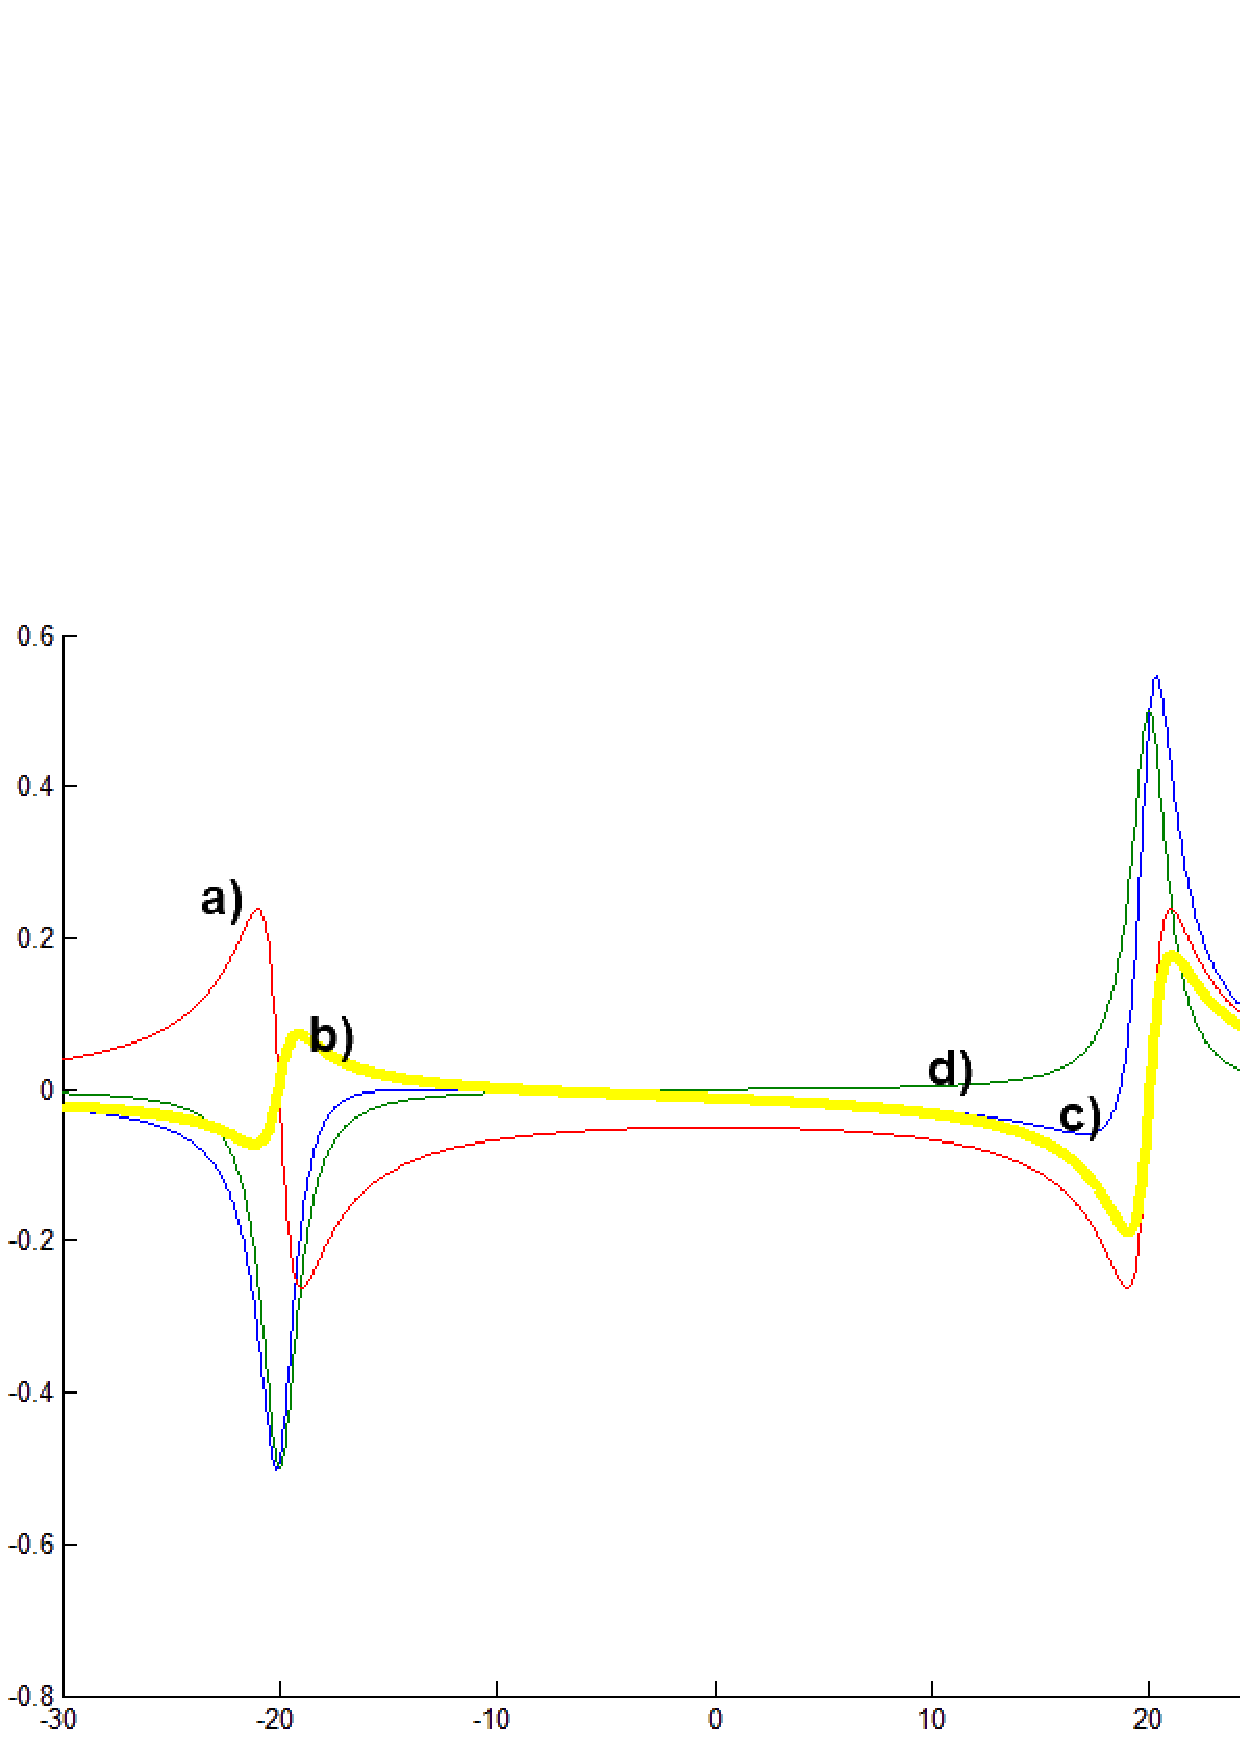
\includegraphics[width=150mm]{img/htran_lin.png}
  \caption{The Figure presents the results of the HTRAN method applied for the simple linear model. We have used 500 points (N = 500).
  Results are plotted together 
   a) The plot of the real part of $\chi (\omega )$ 
   b) absolute error plot (c-plot minus d-plot) 
   c) imaginary part of $\chi (\omega )$ obtained with the Hilbert transform of a-plot 
   d) imaginary part of $\chi (\omega )$ calculated analytically. \label{eq:htran_lin}
  }
\end{figure}

\subsection{HTRAN for simple nonlinear model - results} \label{chap:htran_nlo}

We remind the equation for the pump-and-probe susceptibility model (\ref{eq:physical_pnp_equation}): 

\begin{multline} \label{eq:htran_fparameters}
  \chi_{pp} (\delta ) = \frac {G\,{n_{0}}\,{\gamma_{ba}}}{\Delta + \delta + I\,\eta } \\
    \left(  
    	1 - \frac{{\Omega_{1}}^{2}\,(\Delta - \delta + I \, \eta ) \, (\delta + 2 \, I \, \eta )}
    	         {(\Delta  - I \, \eta) \, ((\delta + I \, \theta ) \, (\delta + \Delta + I \, \eta ) 
    	           \, (\delta - \Delta  + I\,\eta ) - 2 \, {\Omega_{1}}^{2} \, (\delta  + I \, \eta ))} 
    \right) 
\end{multline}

and we have assign the values for the constants:
\begin{tabular}{r r l}
  $G$           & $=$ & $1$, \\
  $\gamma_{ba}$ & $=$ & $1$, \\
  $n_0$         & $=$ & $1$, \\
  $\Delta$      & $=$ & $1.3$, \\
  $\eta$        & $=$ & $1$, \\
  $\theta$      & $=$ & $1.4$, \\
  $\Omega_{1}$  & $=$ & $4.3$. \\
\end{tabular}

The results for such set of parameters are shown on Figure (\ref{fig:htran_pnp_2d}).

\begin{figure}
  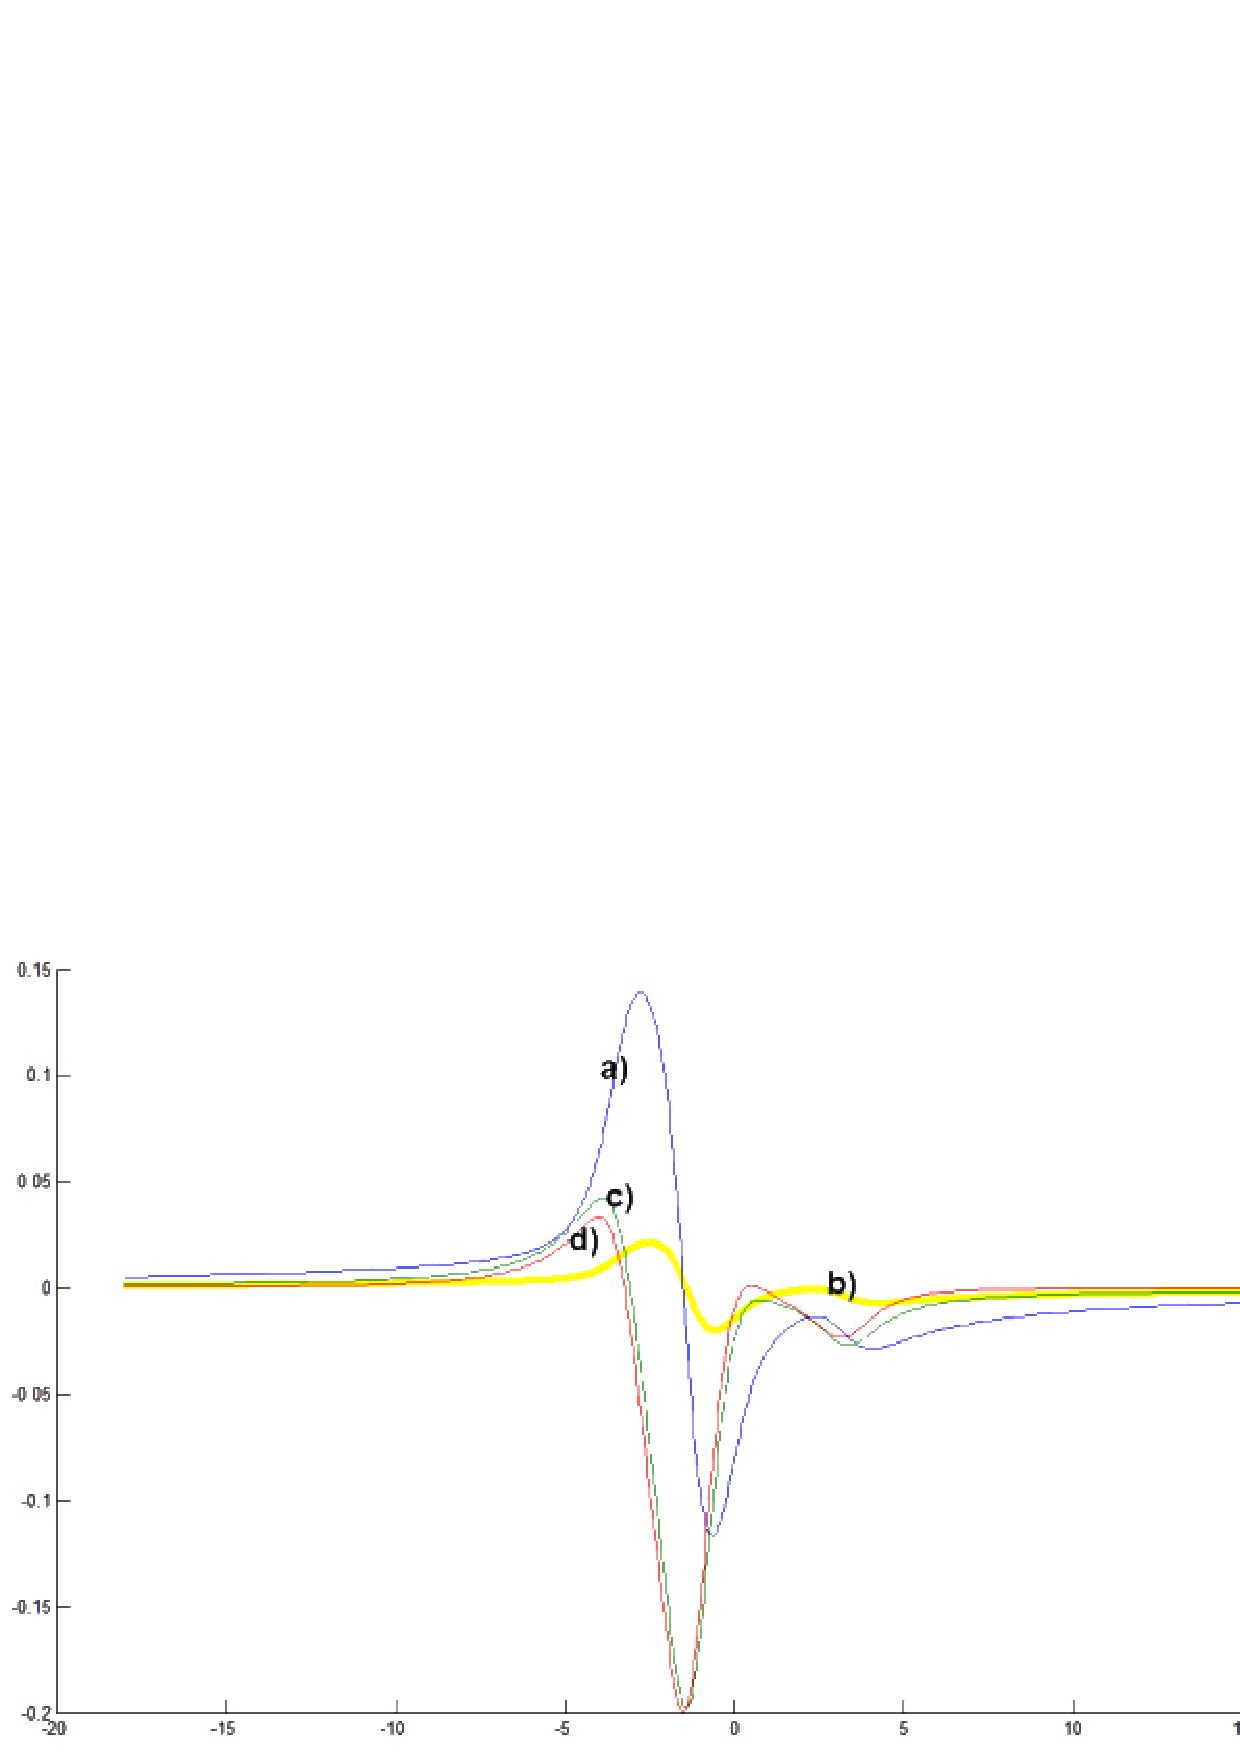
\includegraphics[width=150mm]{img/htran_pnp_2d.png}
  \caption{The Figure presents the results of the HTRAN method applied for the pump-and-probe model. We have used 500 points (N =
  500). Results are plotted together 
    a) The plot of the real part of $\chi_{pp} (\omega )$ 
    b) absolute error plot (c-plot minus d-plot) 
    c) imaginary part of $\chi_{pp} (\omega )$
    d) imaginary part of ${\chi_{pp}}(\omega )$ calculated analytically.
    \label{fig:htran_pnp_2d}}
\end{figure}

The resulted b-plot seems to be a not-so-bad introduction into the Hilbert transform evaluation, as we have only employed the
simple Simpson's rule. We would also like to perform the three-dimensional analysis of the assumed pump-probe susceptibility, so we
employ the (\ref{eq:dconclude_imag}) and (\ref{eq:dconclude_real}) equations for each frequency. The obtained three-dimensional shapes are
similar to the original ones, but we have received a huge relative error as presented in Figure (\ref{fig:htran_pnp_3derr}).

\begin{figure}
  \begin{center}
    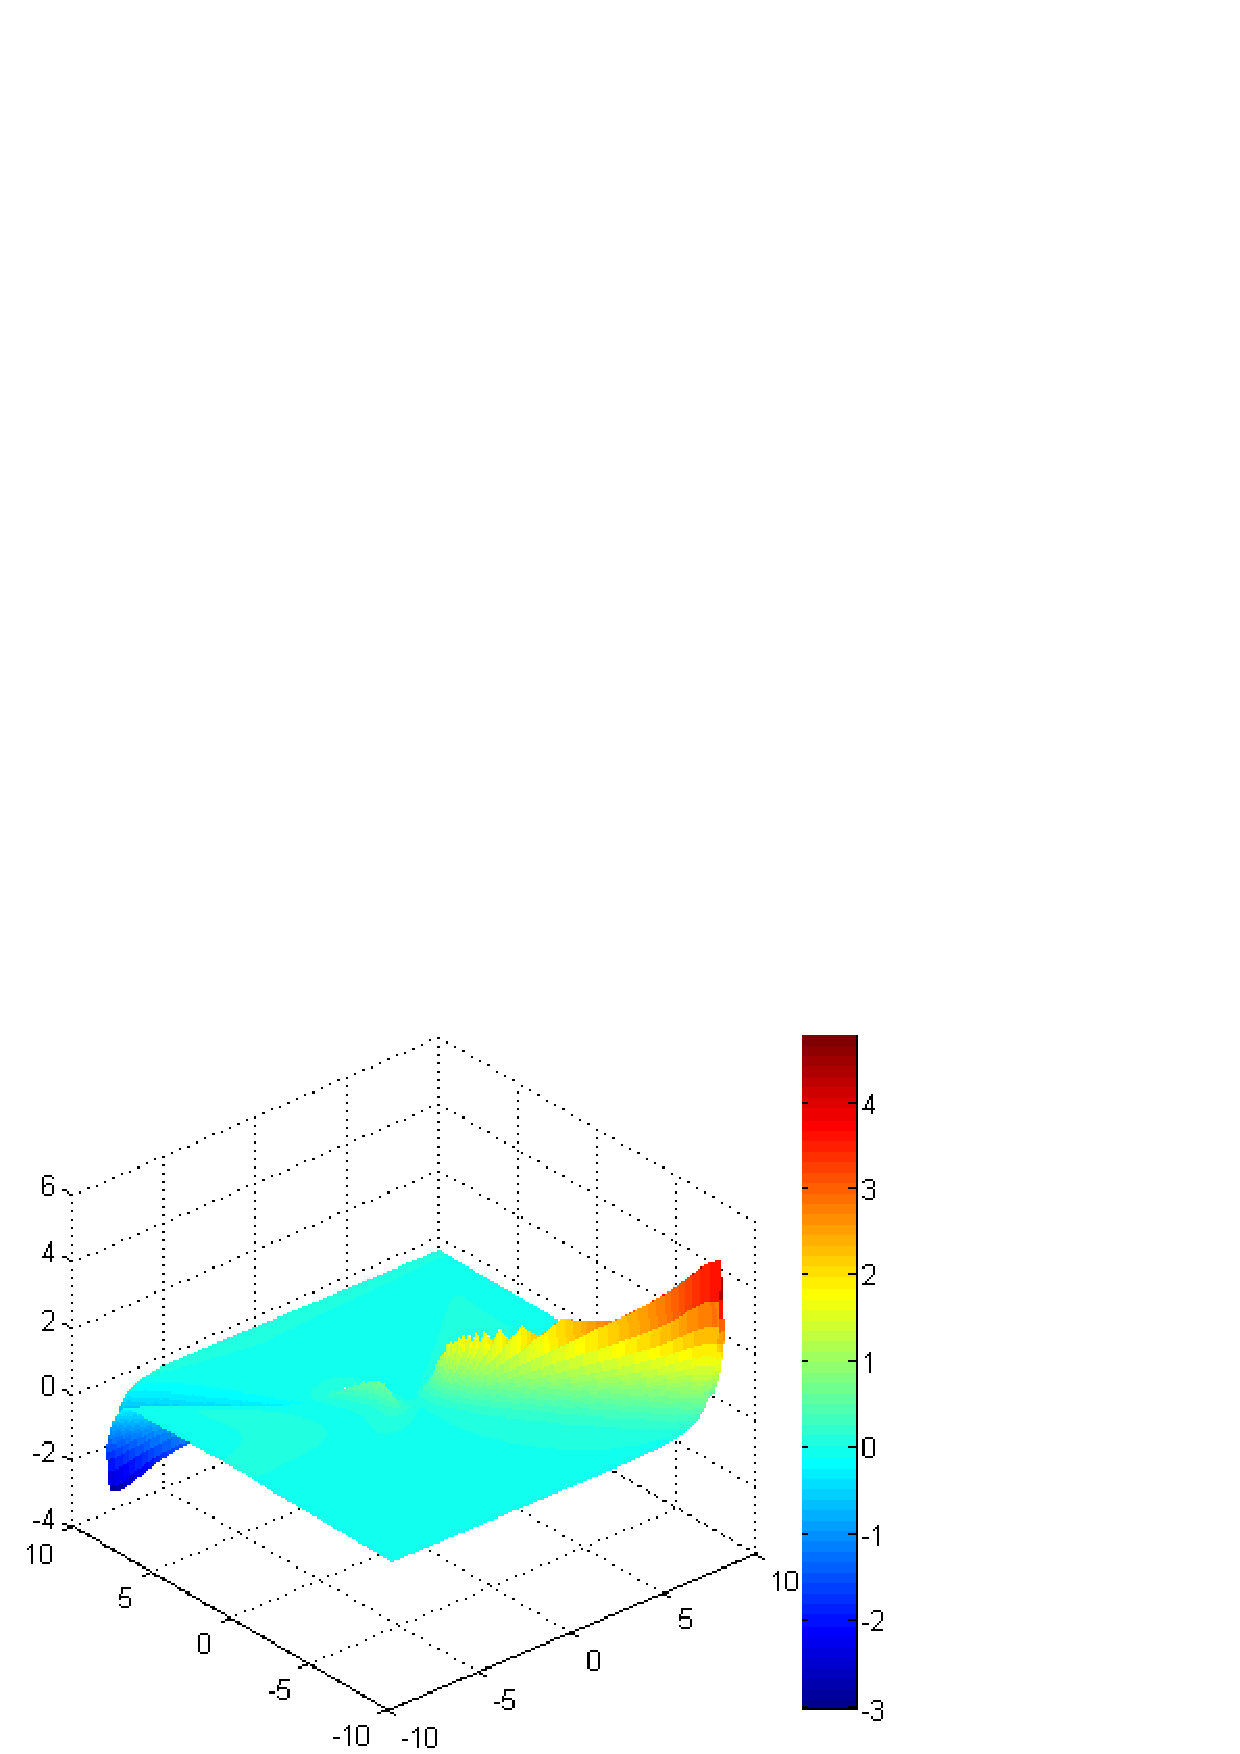
\includegraphics{img/htran_pnp_3derr.png}
    \caption{The Figure presents the combined relative error for the results of the HTRAN method applied for the two-dimensional
    pump-and-probe model. The light-cyan colour shows the area of error below 100\%. 
    \label{fig:htran_pnp_3derr}}
  \end{center}
\end{figure} % which is not very bad, but there are areas with error  more above 100

Let us remind and simplify the wave-mixing model stated in the Chapter (\ref{chap:physical_fm}):

\begin{equation} \label{eq:htran_fm}
	\chi_{mix} (\delta) =
      \frac { \text{ const } ( - \delta - \Delta - \frac{i}{ { T_{2} } } ) \, ( \delta  + \frac{2 \, i} { { T_{2} } } ) }
            { ( \Delta + \frac {i}{ { T_{2} } } ) \, ( \Delta  + \delta  + \frac {i}{ { T_{2} } } ) \, { \mathrm{D} } ^ {*} (\delta) },
\end{equation}

We perform the evaluation for the wave-mixing model as stated in the model described by (\ref{eq:feff3_plus}). We expand this
equation to resolve the complex conjugate of the function D, and the resulting function is:

\begin{equation} \label{eq:htran_feffexp}
  \chi_{mix}( \delta ) = 
    \frac{ \text{ const } 
           ( - \delta - \Delta - \frac {i}{ T_{2} } ) 
           ( \delta + \frac{2 \, i}{ T_{2} } ) 
	       ( \Delta + \frac {i}{ T_{2} } ) ^ {-1} 
	       ( \Delta + \delta + \frac {i}{ T_{2} } ) ^ {-1} } 
	     { ( \delta^{3} 
	       - \frac{2 \, i \, \delta^{2} } { T_{2} } 
	       - \delta \,\Delta^{2} 
	       - \frac {2\,i\,\delta } { T_{1}  \, T_{2} } 
	       - \frac{ \delta }{ {T_{2} } ^ {2} } 
	       + \frac { \delta^{2} } { T_{1} } 
	       - \frac { \Delta^{2} } { T_{1} } 
	       - \frac {1}{ { T_{1} } \, {T_{2}}^{2}} 
	       - {\Omega_{2}}\,\delta  
	       + \frac { \Omega_{2} \, i} { T_{2} } ) }
\end{equation}	     

With such a complex function we obtain the two and three dimensional results presented on Figure (\ref{fig:htran_mix_2d}).
 
\begin{figure}
  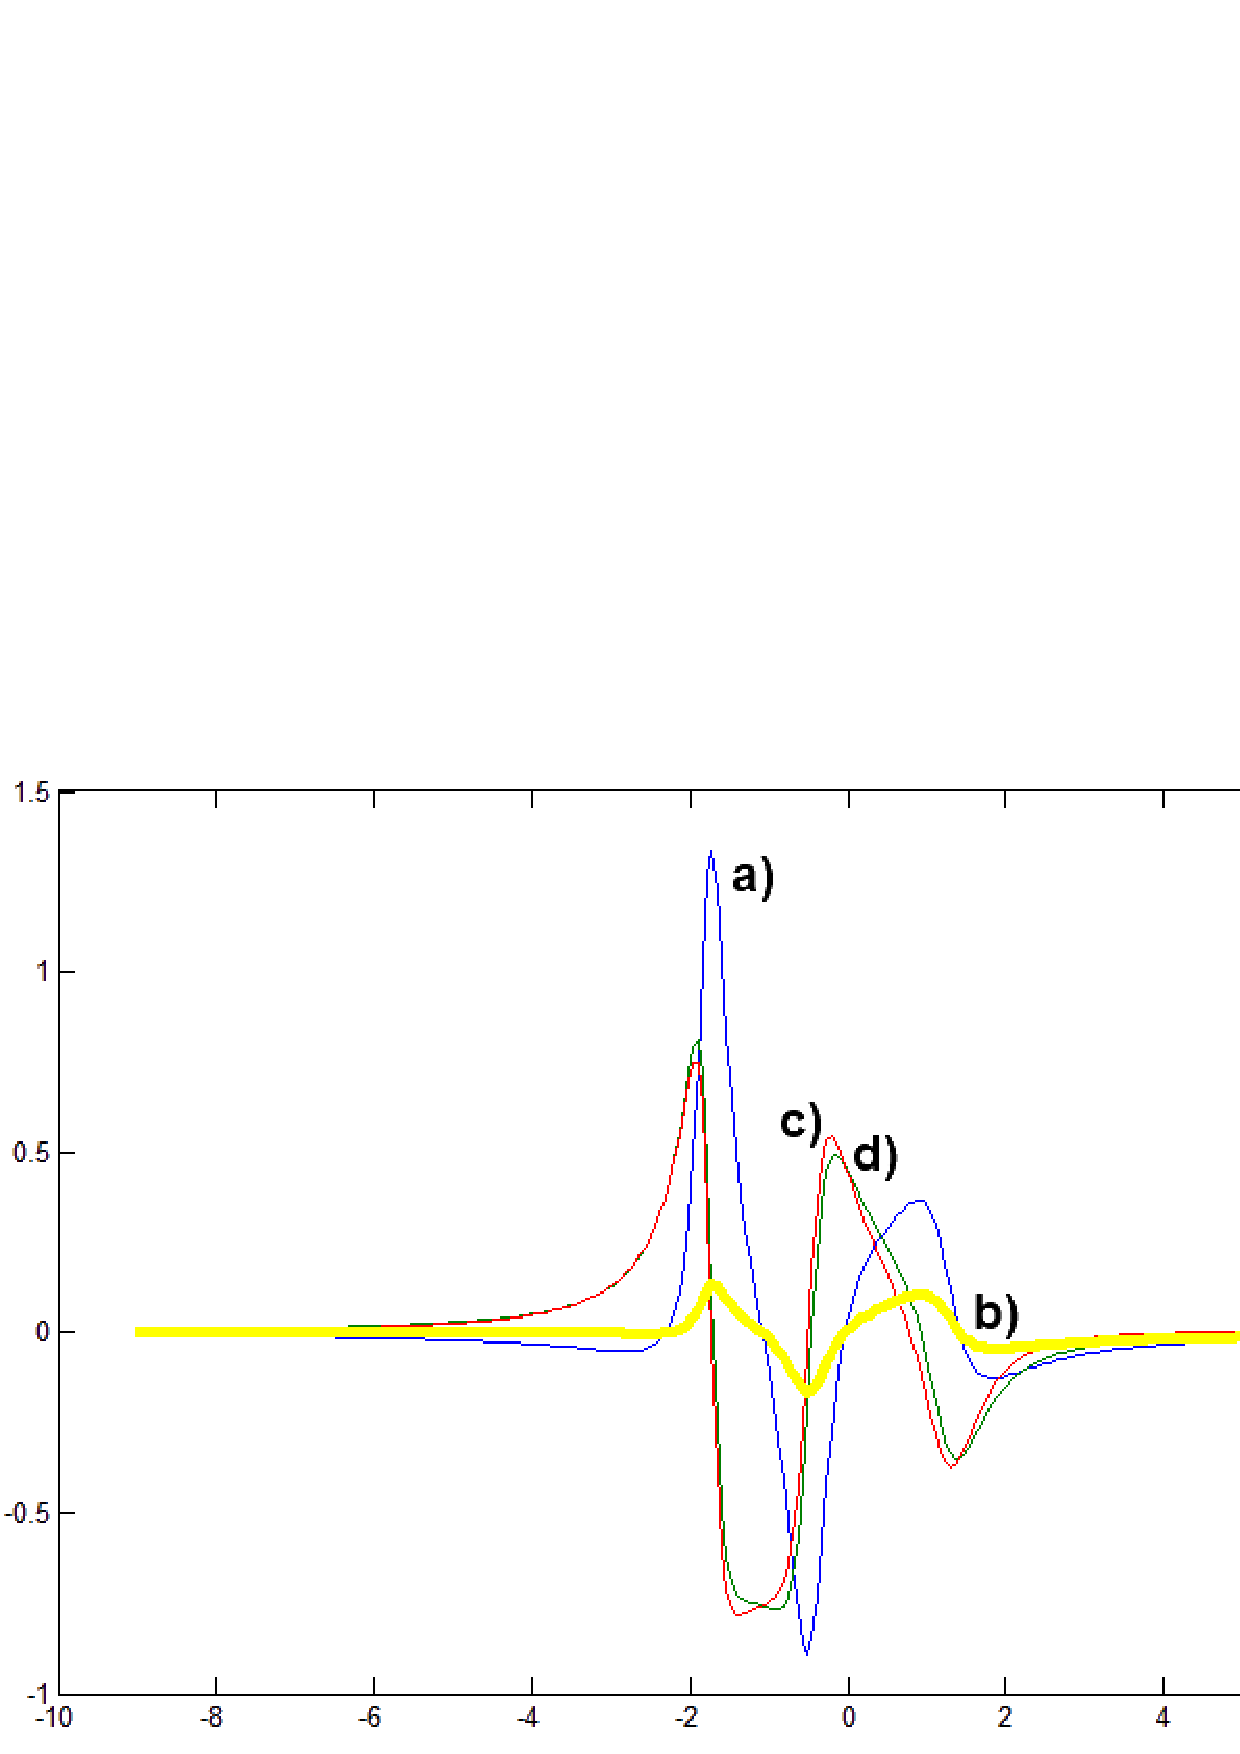
\includegraphics[width=150mm]{img/htran_fmix_2d.png}
  \caption{The Figure presents the combined relative error for the results of the HTRAN method applied for the
  two-dimensional wave-mixing model.
   a) The plot of the real part of ${\chi_{mix}}(\omega )$
   b) absolute error plot (c-plot minus d-plot)
   c) (red) imaginary part of  ${\chi_{mix}}(\omega )$
   d) (grey) imaginary part of ${\chi_{mix}}(\omega )$ calculated analytically.
   \label{fig:htran_mix_2d} }
\end{figure}

While the obtained three-dimensional shape looks very similar to those obtained analytically, the relative error still remains huge for some
areas - see Figure (\ref{fig:htran_fmix_3derr}).

\begin{figure}
  \begin{center}
    \includegraphics{img/htran_fmix_3derr.png}
    \caption{The Figure presents the combined relative error for the real part of nonlinear susceptibility
    ${\chi_{mix}}(\delta )$ describing the wave-mixing process. \label{fig:htran_fmix_3derr}}
  \end{center}    
\end{figure}

\subsection{HTRAN for simple quantum-perturbative model - results} \label{chap:htran_quantum}

We will use the models already prepared for both linear and second-order nonlinear susceptibilities defined in Chapter
(\ref{chap:problem_quantum}).

\begin{equation} \label{eq:htran_qpeq}
  \chi_{1, \,qp}(\omega ) = 
  \frac{N}{\varepsilon_0\,\hbar} \sum_{n=1}^{2}\,(\frac {{\mu_{1, \,n}}\,{\mu_{2, \,n}}}{{\Omega_{n}} - \omega -
  i\,{\gamma_{n}}} + \frac {{\mu_{2, \,n}}\,{\mu_{1, \,n}}}{{\Omega_{n}} + \omega + i\,{\gamma_{n}}}) ,
\end{equation}

We have used the constants' values defined in (\ref{eq:htran_qp1_const}). 

\begin{equation} \label{eq:htran_qp1_const}
  \mu = \begin{bmatrix} 
          1  & 3 \\ 
          -1 & -2
        \end{bmatrix},
  \Omega = \begin{bmatrix}
           3 \\ 16
           \end{bmatrix},
  \gamma = \begin{bmatrix}
           1 \\ 2
           \end{bmatrix}, 
  N = 5, 
  \varepsilon_0 = 1, 
  h = -1.
\end{equation}

\begin{figure} 
  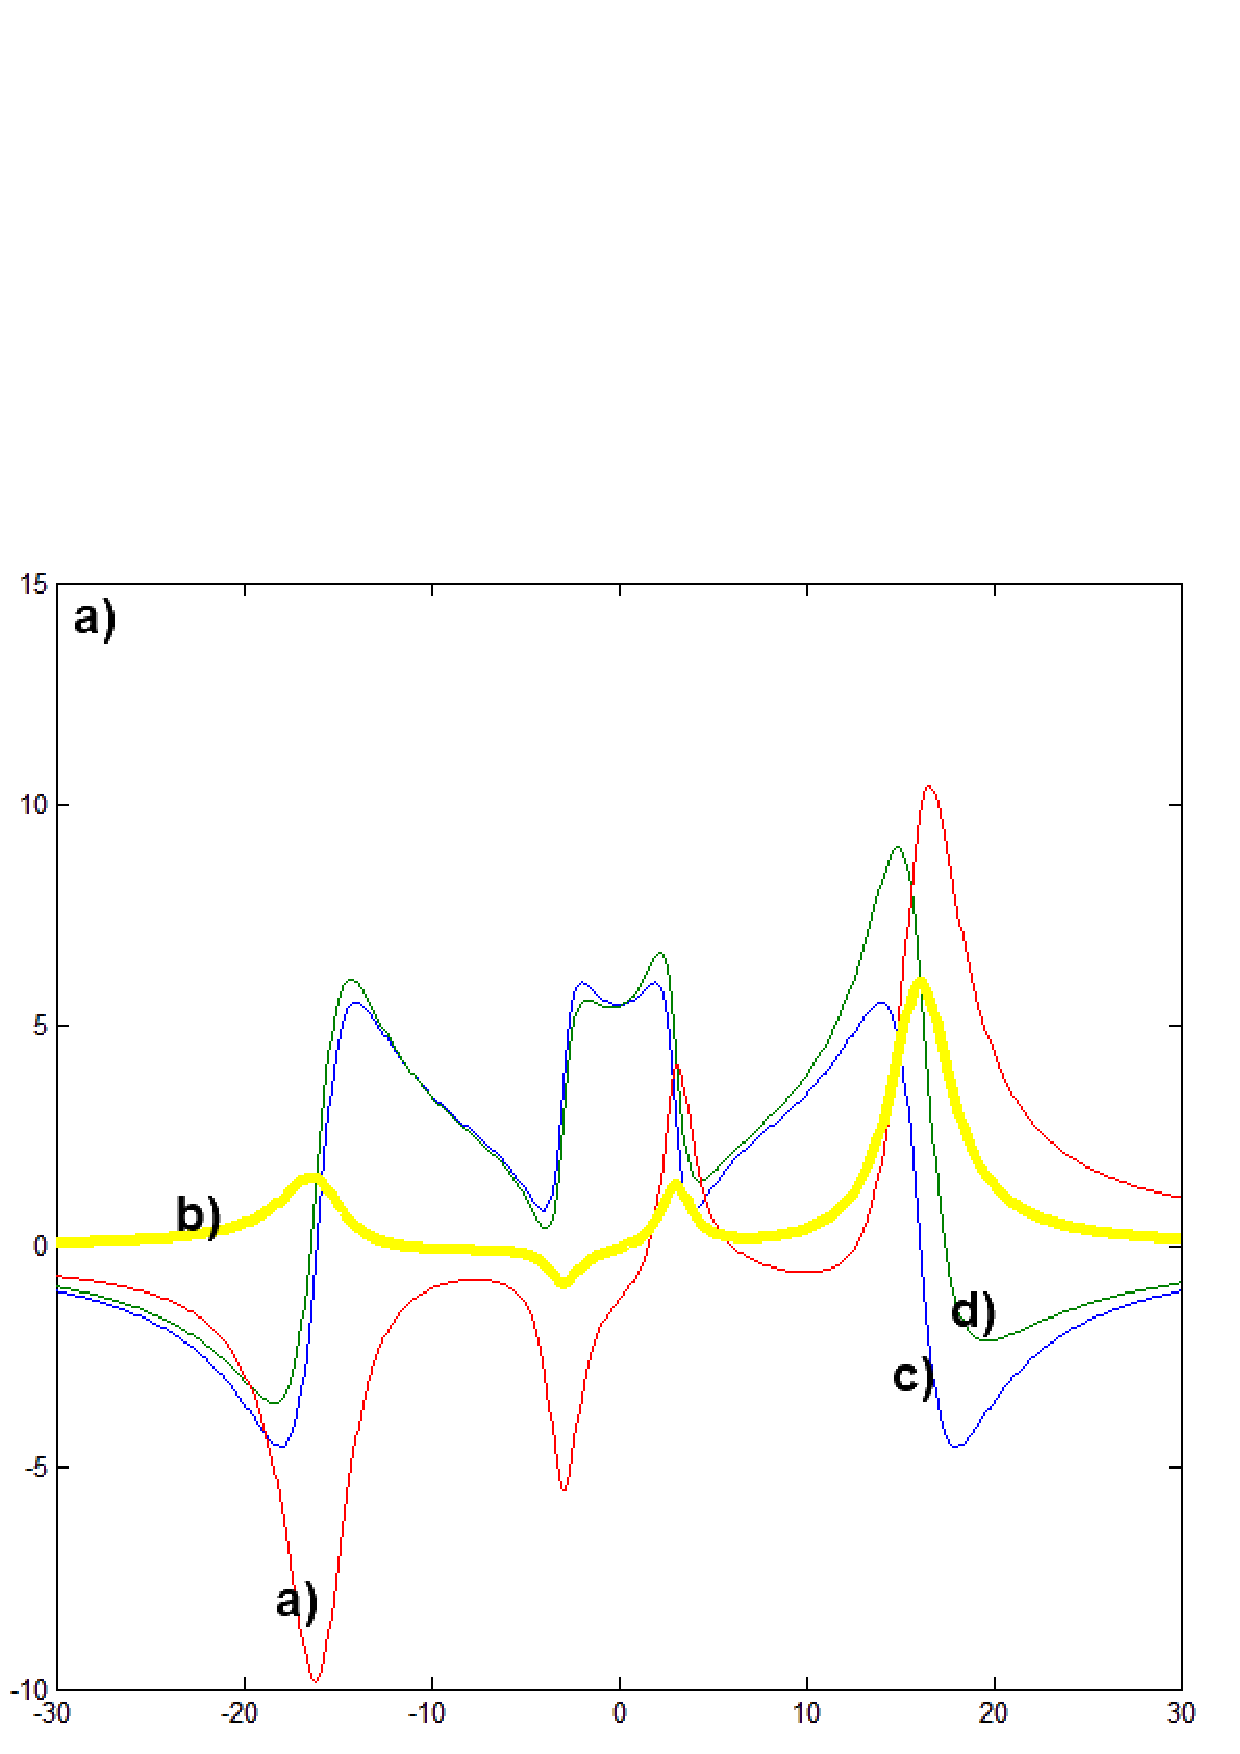
\includegraphics[width=70mm]{img/htran_qp_2da.png} 
  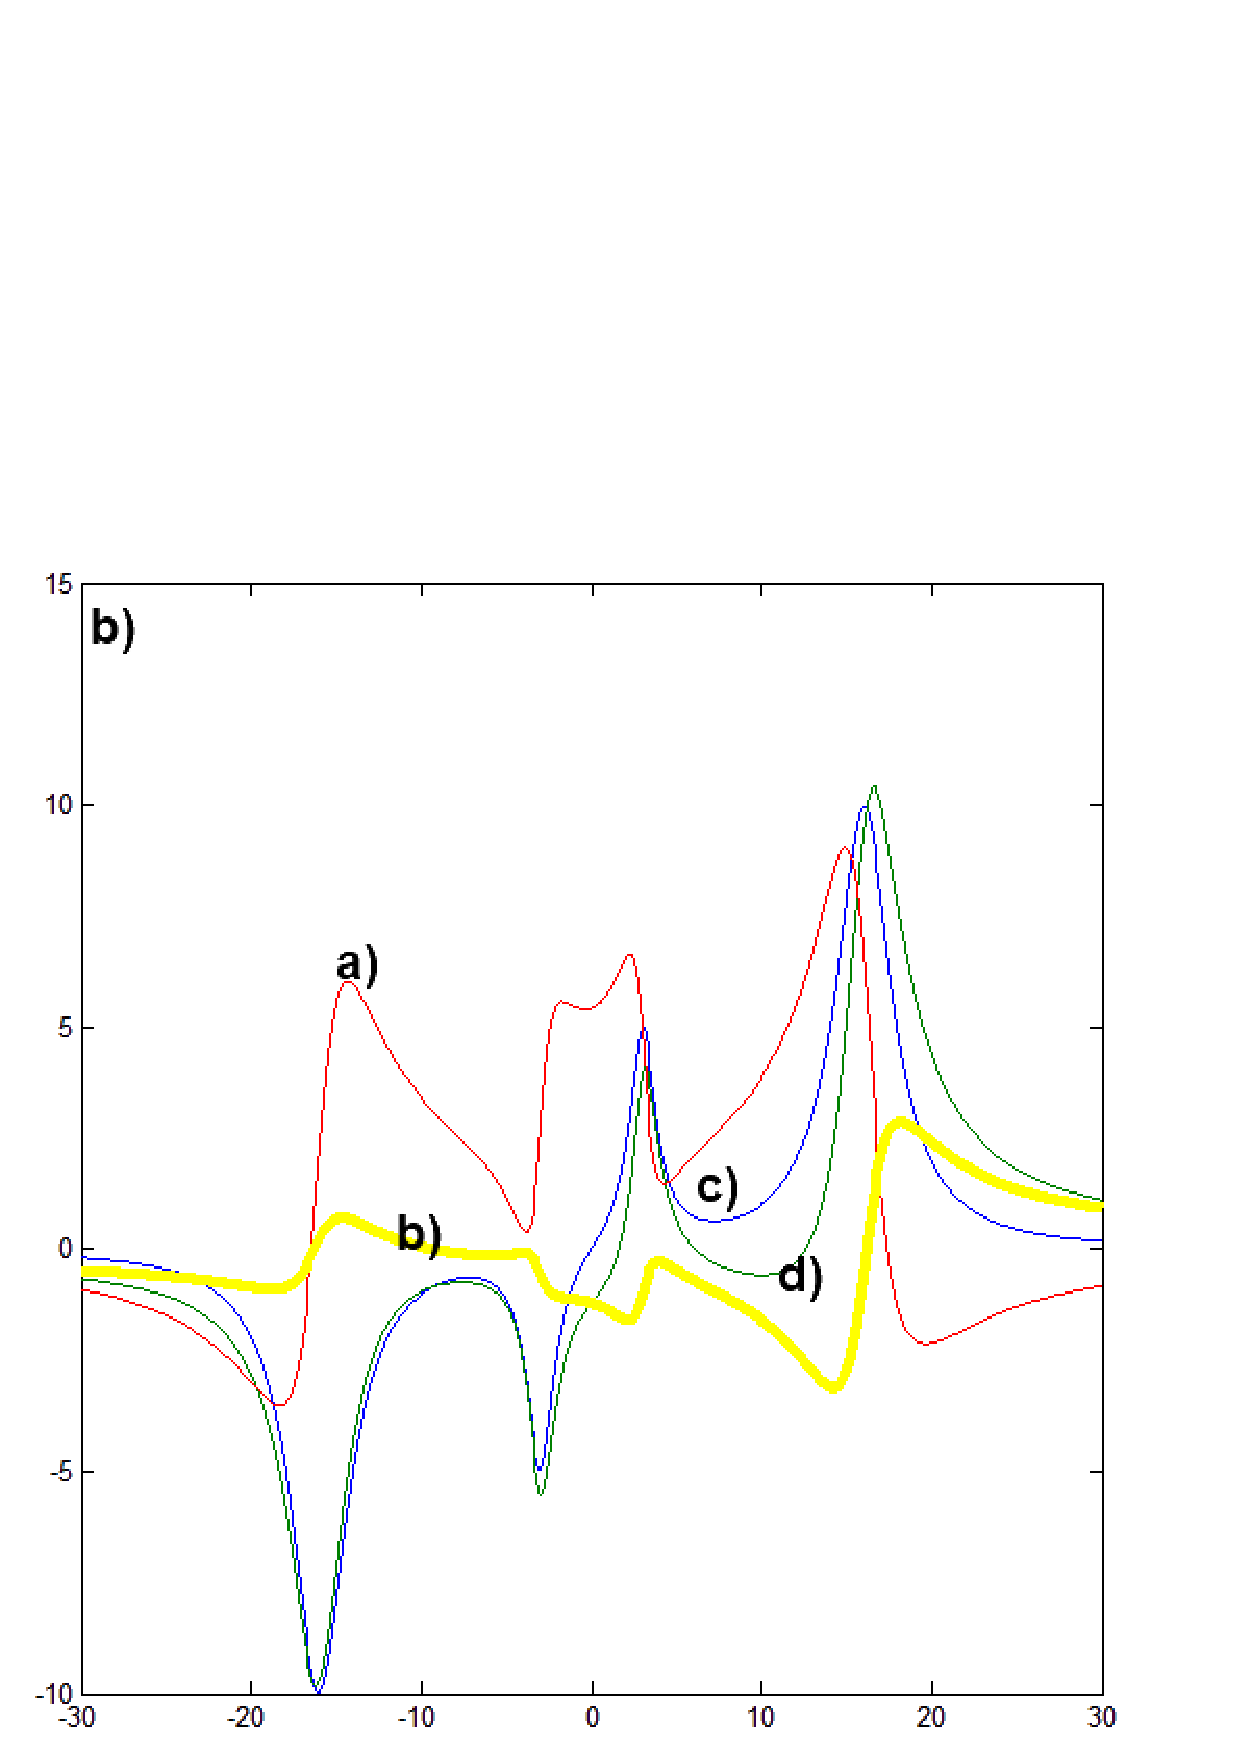
\includegraphics[width=70mm]{img/htran_qp_2db.png}  
  \caption{The Figure presents the results of the HTRAN method applied for the linear quantum-perturbative model. The results for both real
  and imaginary values are plotted together on Figures a and b:
  a.a) The plot of the imaginary part of ${\chi_{1, \, qp}}(\omega )$ 
  a.b) absolute error plot (a.d-plot minus a.c-plot) 
  a.c) real part of ${\chi_{1, \, qp}}(\omega )$ calculated analytically
  a.d) real part of ${\chi_{1, \, qp}}(\omega )$ obtained with the Hilbert transform of a-plot
  b.a) The plot of the real part of ${\chi_{1, \, qp}}(\omega )$
  b.b) absolute error plot (b.d-plot minus b.c-plot)  
  b.c) imaginary part of ${\chi_{1, \, qp}}(\omega )$ calculated analytically 
  b.d) imaginary part of ${\chi_{1, \, qp}}(\omega )$ obtained with the Hilbert transform of a-plot 
  \label{fig:htran_qp_2d}}
\end{figure}

Results are gathered on Figure (\ref{fig:htran_qp_2d}). As we can see - the absolute error is quite huge, but on the other hand the
pairs of plots (a.c) with (a.d) and (b.c) with (b.d) have at least similar shapes. As for the simplest applied method these results can be
satisfactory in case we only would like to initially reject or accept the investigated model. In case we need much higher accuracy, we will
need to search for more precise methods.

In the equation (\ref{eq:htran_qp_reminder}) we remind the second-order quantum-perturbative sum-over-states model from the Chapter
(\ref{chap:problem_quantum}). 

\begin{equation} \label{eq:htran_qp_reminder}
  \begin{split} 
     & \chi_{2, \, qp}(\omega_1, \, \omega_2 ) = 
    \frac{N} {2 \, \varepsilon_0 \, h^2} \sum_{n=1}^{2} \sum_{m=1}^{2} \sum_{l=1}^{2} 
    \\ ( & \frac {{\mu_{ln}} \, {\mu_{nm}} \, {\mu_{ml}} \, ({\Omega_{ml}} - \omega_1 - i \, {\gamma_{ml}})^{-1} }
        {({\Omega_{nl}} - \omega_1 - \omega_2 - i \, {\gamma_{nl}}) }
       + \frac {{\mu_{ln}} \, {\mu_{nm}} \, {\mu_{ml}} \, ({\Omega_{ml}} - \omega_2 - i \, {\gamma_{ml}})^{-1} }
        {({\Omega_{nl}} - \omega_1 - \omega_1 - i \, {\gamma_{nl}}) } 
    \\ + & \frac {{\mu_{ln}} \, {\mu_{nm}} \, {\mu_{ml}} \, ({\Omega_{nl}} + \omega_2 + i \, {\gamma_{nl}})^{-1} }
        {({\Omega_{mn}} - \omega_1 - \omega_2 - i \, {\gamma_{mn}}) } 
       + \frac {{\mu_{ln}} \, {\mu_{nm}} \, {\mu_{ml}} \, ({\Omega_{nl}} + \omega_2 + i \, {\gamma_{nl}})^{-1} }
        {({\Omega_{mn}} - \omega_1 - \omega_2 - i \, {\gamma_{mn}}) } 
    \\ + & \frac {{\mu_{ln}} \, {\mu_{nm}} \, {\mu_{ml}} \, ({\Omega_{ml}} - \omega_1 - i \, {\gamma_{ml}})^{-1} }
        {({\Omega_{nm}} + \omega_1 + \omega_2 + i \, {\gamma_{nm}}) } 
       + \frac {{\mu_{ln}} \, {\mu_{nm}} \, {\mu_{ml}} \, ({\Omega_{ml}} - \omega_1 - i \, {\gamma_{ml}})^{-1} }
        {({\Omega_{nm}} + \omega_1 + \omega_2 + i \, {\gamma_{nm}}) } 
    \\ + & \frac {{\mu_{ln}} \, {\mu_{nm}} \, {\mu_{ml}} \, ({\Omega_{nl}} + \omega_1 + i \, {\gamma_{nl}})^{-1} }
        {({\Omega_{ml}} + \omega_1 + \omega_2 + i \, {\gamma_{ml}}) } 
       + \frac {{\mu_{ln}} \, {\mu_{nm}} \, {\mu_{ml}} \, ({\Omega_{nl}} + \omega_2 + i \, {\gamma_{nl}})^{-1} }
        {({\Omega_{ml}} + \omega_1 + \omega_2 + i \, {\gamma_{ml}})}).
  \end{split} 
\end{equation}

We have applied the following constants' values: 

\begin{equation} \label{eq:htran_qp_constant}
  \mu = \begin{bmatrix}
          1, &  3 \\
         -1, & -2
        \end{bmatrix}, \,
  \Omega = \begin{bmatrix}
          3, & 16 \\
          4, & 12
        \end{bmatrix}, \,
  \gamma = \begin{bmatrix}
          1, & 2 \\
         -1, & 3
        \end{bmatrix}, \,
  N = 5, \,
  \varepsilon_0 = 1, \, 
  h = -1.
\end{equation}

\begin{figure}
  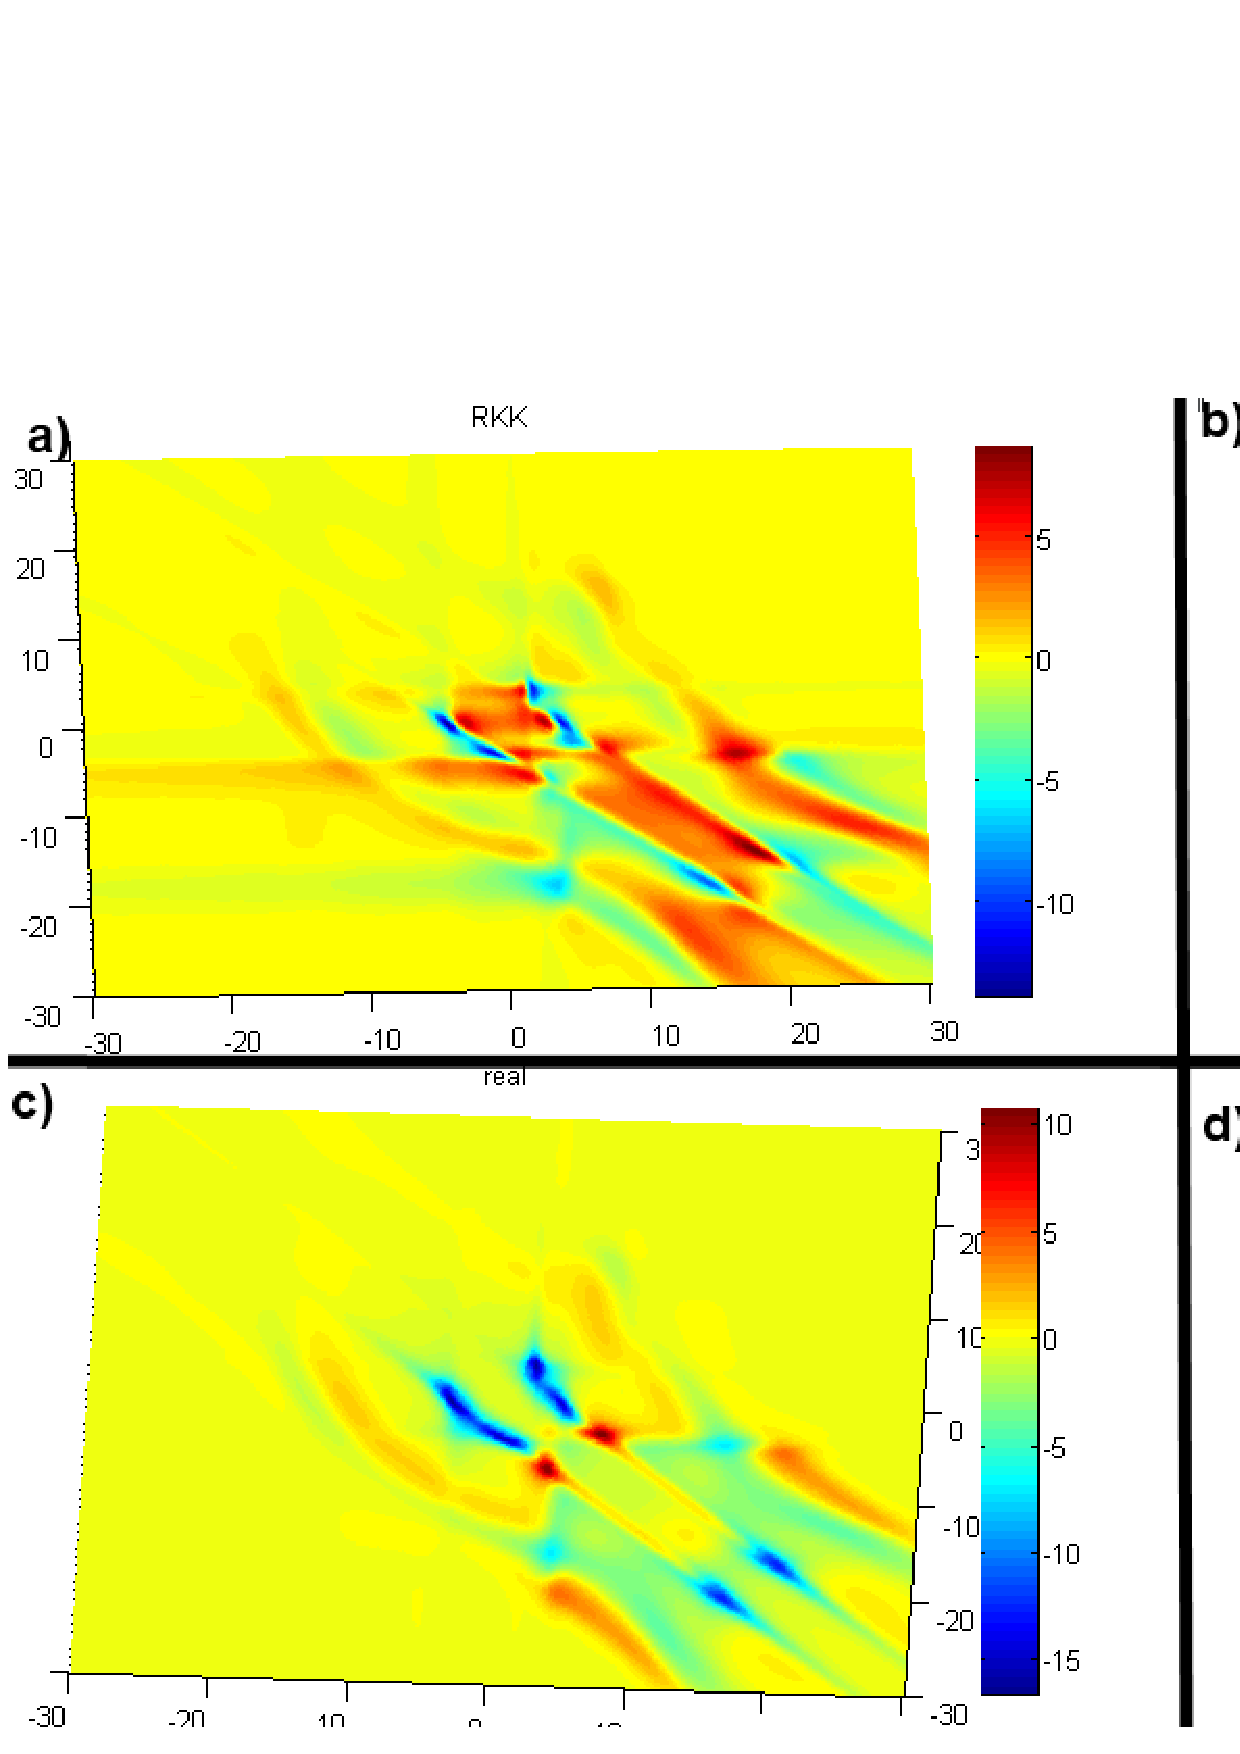
\includegraphics[width=150mm]{img/htran_qp_3d.png}
  \caption{The Figure presents the results of the HTRAN method applied for the second-order nonlinear quantum-perturbative model. Results
  in the three-dimensional-like plot are plotted together.
     a) - The calculated real part of ${\chi_{2, \, qp}}$ 
     b) The calculated imaginary part of ${\chi_{2, \, qp}}$ 
     c) The real part of nonlinear susceptibility ${\chi_{2, \, qp}}$ calculated analytically 
     d) The imaginary part of the nonlinear susceptibility ${\chi_{2, \, qp}}$
     \label{fig:htran_qp_3d}}
\end{figure}

As the equations (\ref{eq:dlucarini_imag}) and (\ref{eq:dlucarini_real}) are symmetric, in the 3-dimensional model we treated the real and
imaginary parts as input and performed the 2-dimensional Hilbert transform in a simplified ``stripe by stripe'' way. Results are
presented in Figure (\ref{fig:htran_qp_3d}). We can see that there is a similarity in obtained plots, but both the relative and absolute
error do not satisfy us at all. Those obtained with 2-dimensional model were more satisfying - see Figure (\ref{fig:htran_qp_2d}).

We have implemented the HTRAN method in the MATLAB \textsuperscript{\textregistered} environment, and its source code is available in
the Appendix A.1.

\section{Newton-Cotes based Hilbert transform (HNC)} \label{chap:nc}

\subsection{Overview of the Newton-Cotes (NC) quadrature of arbitrary degree}  \label{chap:nc_quadrature}

Newton-Cotes formula for numerical integration is taken into consideration. We compare formula for an arbitrary degree - having in
our mind that the choice between formulas of high and low degree must be undertaken with the awareness of numerical errors which
may arise. Newton-Cotes quadrature is a method for numerical integration with equispaced vertices. As we would like to integrate
function $f = f(x)$ within the range $[a, b]$ we introduce the following symbols:

\begin{subequations} \label{eq:nc_parameters}
  \begin{equation}   \label{eq:ncparms_x}
    {x_{n, \,k}}=a + \frac {(b - a)}{n}\,k \,\mbox{ for }\,k = 0, \,1,\,\ldots,\,n
  \end{equation}
  \begin{equation}   \label{eq:ncparms_omega}
    {\omega_{n}}(x) = (x - {x_{n, \,0}})(x - {x_{n, \,1}}),\,\ldots,\,(x - {x_{n, \,n}})
  \end{equation}
  \begin{equation}   \label{eq:ncparms_lambda}
    {\lambda_{n, \,k}}(x)=\frac {{\omega_{n}}(x)}{({\frac {\partial }{\partial x}}\,{\omega_{n}}({x_{n, \,k}}))\,(x - {x_{n,\,k}})}
    \, \mbox{ for}\, k = 0, \,1,\,\ldots,\,n
  \end{equation}
  \begin{equation}   \label{eq:ncparms_a}
    {A_{n, \,k}}=\int_{a}^{b}{\lambda_{n, \,k}}(x)\,dx = \frac {(b - a)\,( - 1)^{(n - k)}}{n\,k\mathrm{!}\,(n - k)\mathrm{!}}
    \int_{0}^{n}\prod_{j=0, \,j \neq k}^{n}\,(t - j)\,dt\, \mbox{ for }\,k = 0, \,1,\,\ldots,\,n
  \end{equation}  
\end{subequations} 

With parameters defined in this way, the quadrature in sense of Newton-Cotes is defined as following:

\begin{equation} \label{eq:nc_mainequation}
   NC_{n} (f) = { A_{n, \, k} } \sum_{ k = 0 }^{n} \, f \, (a + \frac {(b - a)} {n} \, k) . 
\end{equation}

Let's remind the Hilbert transform from the equation (\ref{eq:mathematical_hilbert}):

\begin{equation} \label{eq:nc_hilbert_remind}
	\mathcal{H}[f(x)] = \frac{1}{\pi} \dashint_{ - \infty }^{\infty } \frac{f(\omega)}{(x - \omega)} \, d\omega . 
\end{equation}

\subsection{Our implementation of the Hilbert Transform HNC}  \label{chap:nc_hilbert_transform}

We would like to apply the Newton-Cotes quadrature to calculate the Hilbert transform. Prepared algorithm will consist of two
main steps. In the first step we modify the region under the integral to omit singularities and deal with infinities. To omit the
singularities as the NC quadrature was not designed to be used on singular functions, we will set a small constant value $c_s$ and
perform the integration without including a short region $[x - c_s, x + c_s]$ near the singularity. To deal with the infinities we observe
that near infinities our input function vanishes so without much loss, we will integrate from a finite, starting point $a$ to the ending
point $b$:

\begin{equation}
	\mathcal{H}[f(x)] \approx \frac{1}{\pi} \int_{ a }^{ x - c_s } \frac{ f(\omega) }{ (x - \omega) } \, d\omega 
                           +  \frac{1}{\pi} \int_{ x + c_s }^{ b } \frac{ f(\omega) }{ (x - \omega) } \, d\omega .
\end{equation} 

In the second step, important in our implementation, we are pre\-calculating the $A_{n, \, k}$ matrix described in equation
(\ref{eq:ncparms_a}) within the function \texttt{prevaluateNCTab(n, a, b)}. We are applying the \texttt{maple} function that connects MATLAB
with Maple and gives us the power of both tools. Once we know the $A_{n, \, k}$ matrix, we can perform the step-by-step calculation in the
\texttt{doStep(fun, a, b, nosteps, tab)} function, which is called with a different number of steps (described with the \texttt{nosteps}
parameter) in the parent loop as long as we demand better precision, related to the tolerance (\texttt{tol}) parameter.

The full algorithm is presented in the Appendix A.2 with the additional comments. 

\subsection{NC for simple linear model - results} \label{chap:nc_lin}

As the prepared numeric method depends on many input parameter arguments, we have tried to perform the evaluation in many different
cases, some of those results are stated below. We have used the same model as in Chapter (\ref{chap:htran_lin}).

\begin{equation} \label{eq:nc_algoritm}
  \chi (\omega ) \approx \frac { - 20}{(\omega \,i + 1 - 20\,i)\,(\omega \,i + 1 + 20\,i)}
\end{equation} 

Some results has been presented on Figures (\ref{fig:nc_lin1}), (\ref{fig:nc_lin2}), (\ref{fig:nc_lin3}) and (\ref{fig:nc_lin4})

\begin{figure}
  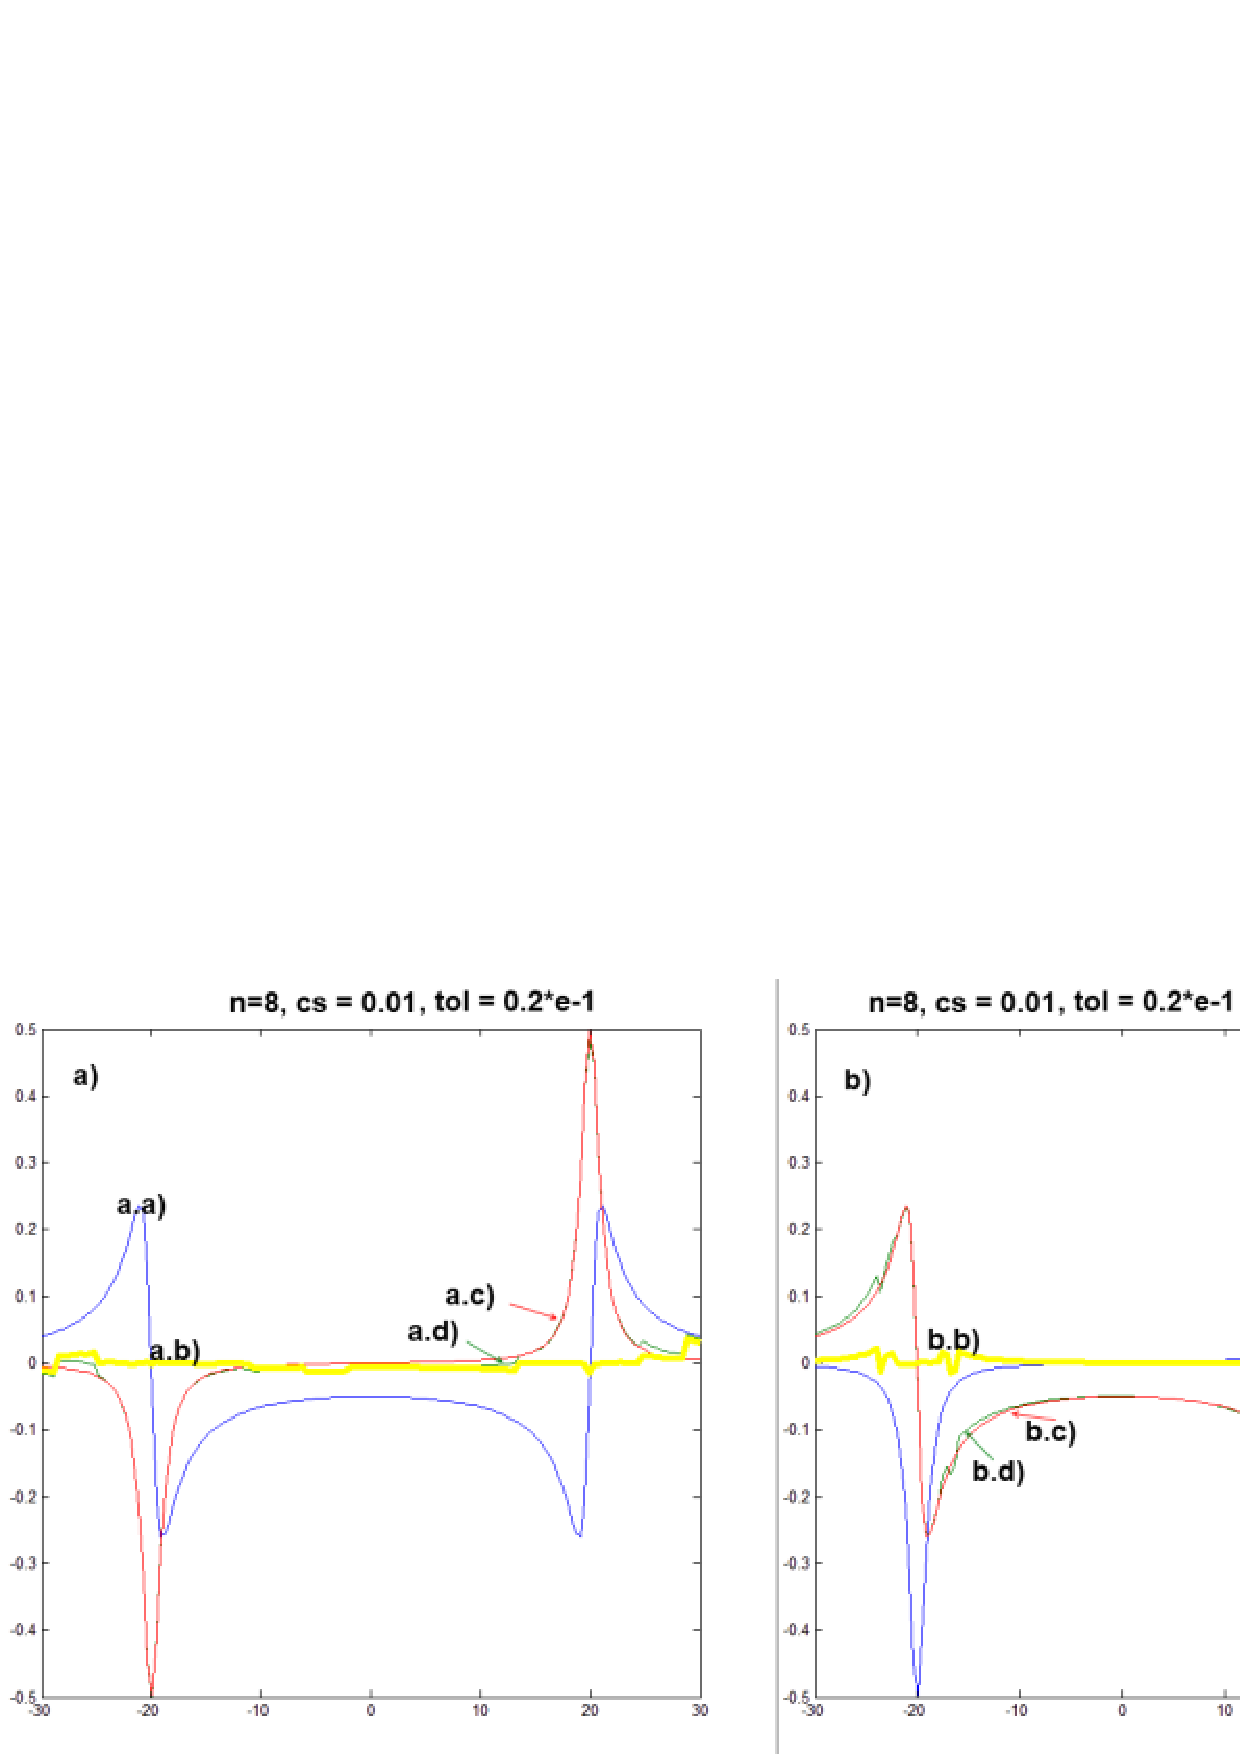
\includegraphics[width=150mm]{img/nc_lin1.png}
   \caption{ The Figure presents the first of four results of the NC Hilbert Transform method applied for the simple linear model. Results
   are plotted together. Calculations were performed with the parameters ($n = 8, \, c_s = \mbox{.1e-1}, \, tol = \mbox{.2e-1})$. Tol -
   parameter describes the error tolerance:
     a.a) The plot of the real part of $\chi (\omega )$ 
     a.b) absolute error plot (a.d-plot minus a.c-plot) 
     a.c) imaginary part of $\chi (\omega )$ calculated analytically 
     a.d) imaginary part of $\chi (\omega )$ obtained with the NC Hilbert transform of a.a-plot, 
     b.a) The plot of the imaginary part of $\chi (\omega )$ 
     b.b) absolute error plot (b.d-plot minus b.c-plot) 
     b.c) real part of $\chi (\omega )$ calculated analytically 
     b.d) real part of $\chi (\omega )$ obtained with the NC Hilbert transform of b.a-plot 
     \label{fig:nc_lin1}
  }
\end{figure}

\begin{figure}
  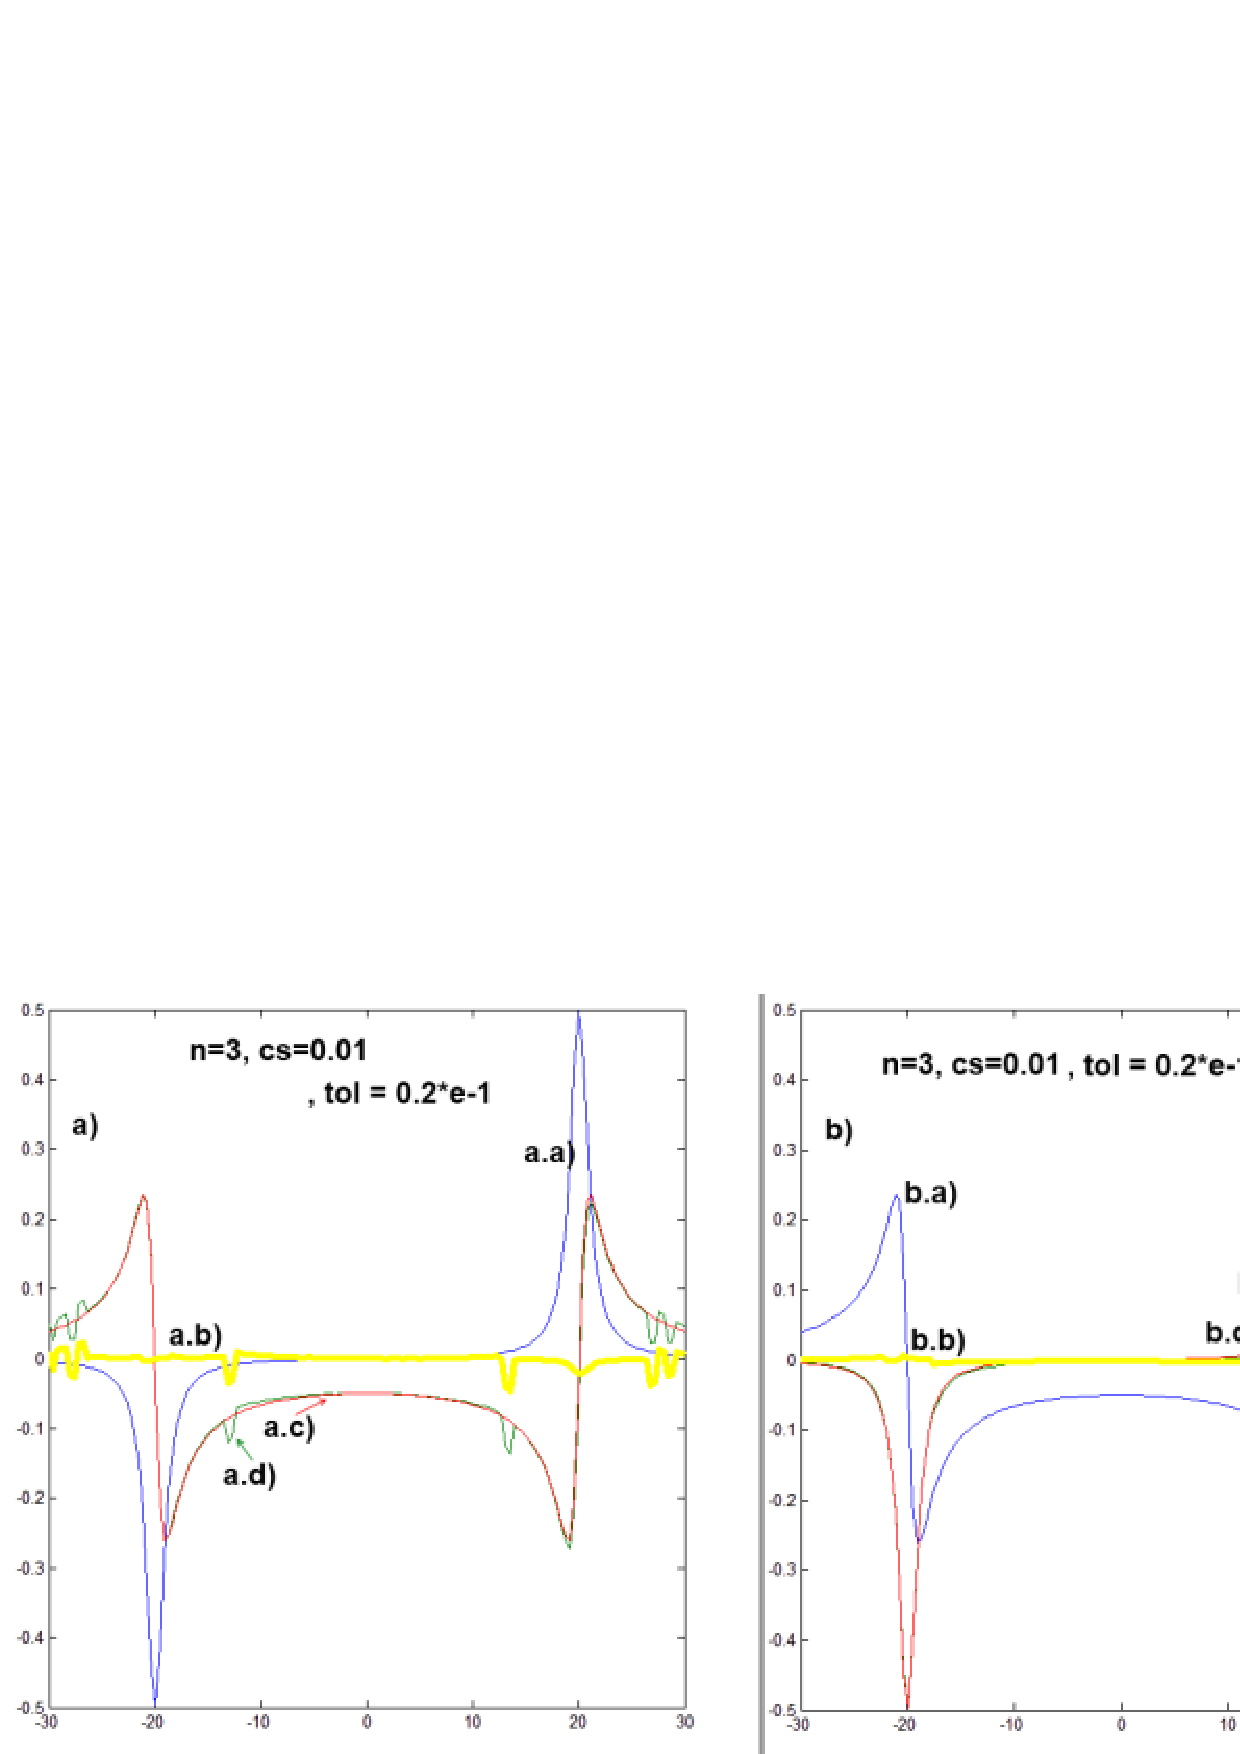
\includegraphics[width=150mm]{img/nc_lin2.png}
  \caption{ The Figure presents the second of four results of the NC Hilbert Transform method applied for the simple linear model.
  Results are plotted together. Calculations were performed with the parameters ($n = 3, \, c_s = \mbox{.1e-1}, \, tol = \mbox{.2e-1})$
     a.a) The plot of the imaginary part of $\chi (\omega )$
     a.b) absolute error plot (a.d-plot minus a.c-plot) 
     a.c) real part of $\chi (\omega )$ calculated analytically 
     a.d) real part of $\chi (\omega )$ obtained with the NC Hilbert transform of a.a-plot, 
     b.a) The plot of the real part of $\chi (\omega )$
     b.b) absolute error plot (b.d-plot minus b.c-plot)
     b.c) imaginary part of $\chi (\omega )$ calculated analytically 
     b.d) imaginary part of $\chi (\omega )$ obtained with the NC Hilbert transform of b.a-plot
     \label{fig:nc_lin2} 
  }
\end{figure}  

\begin{figure}
  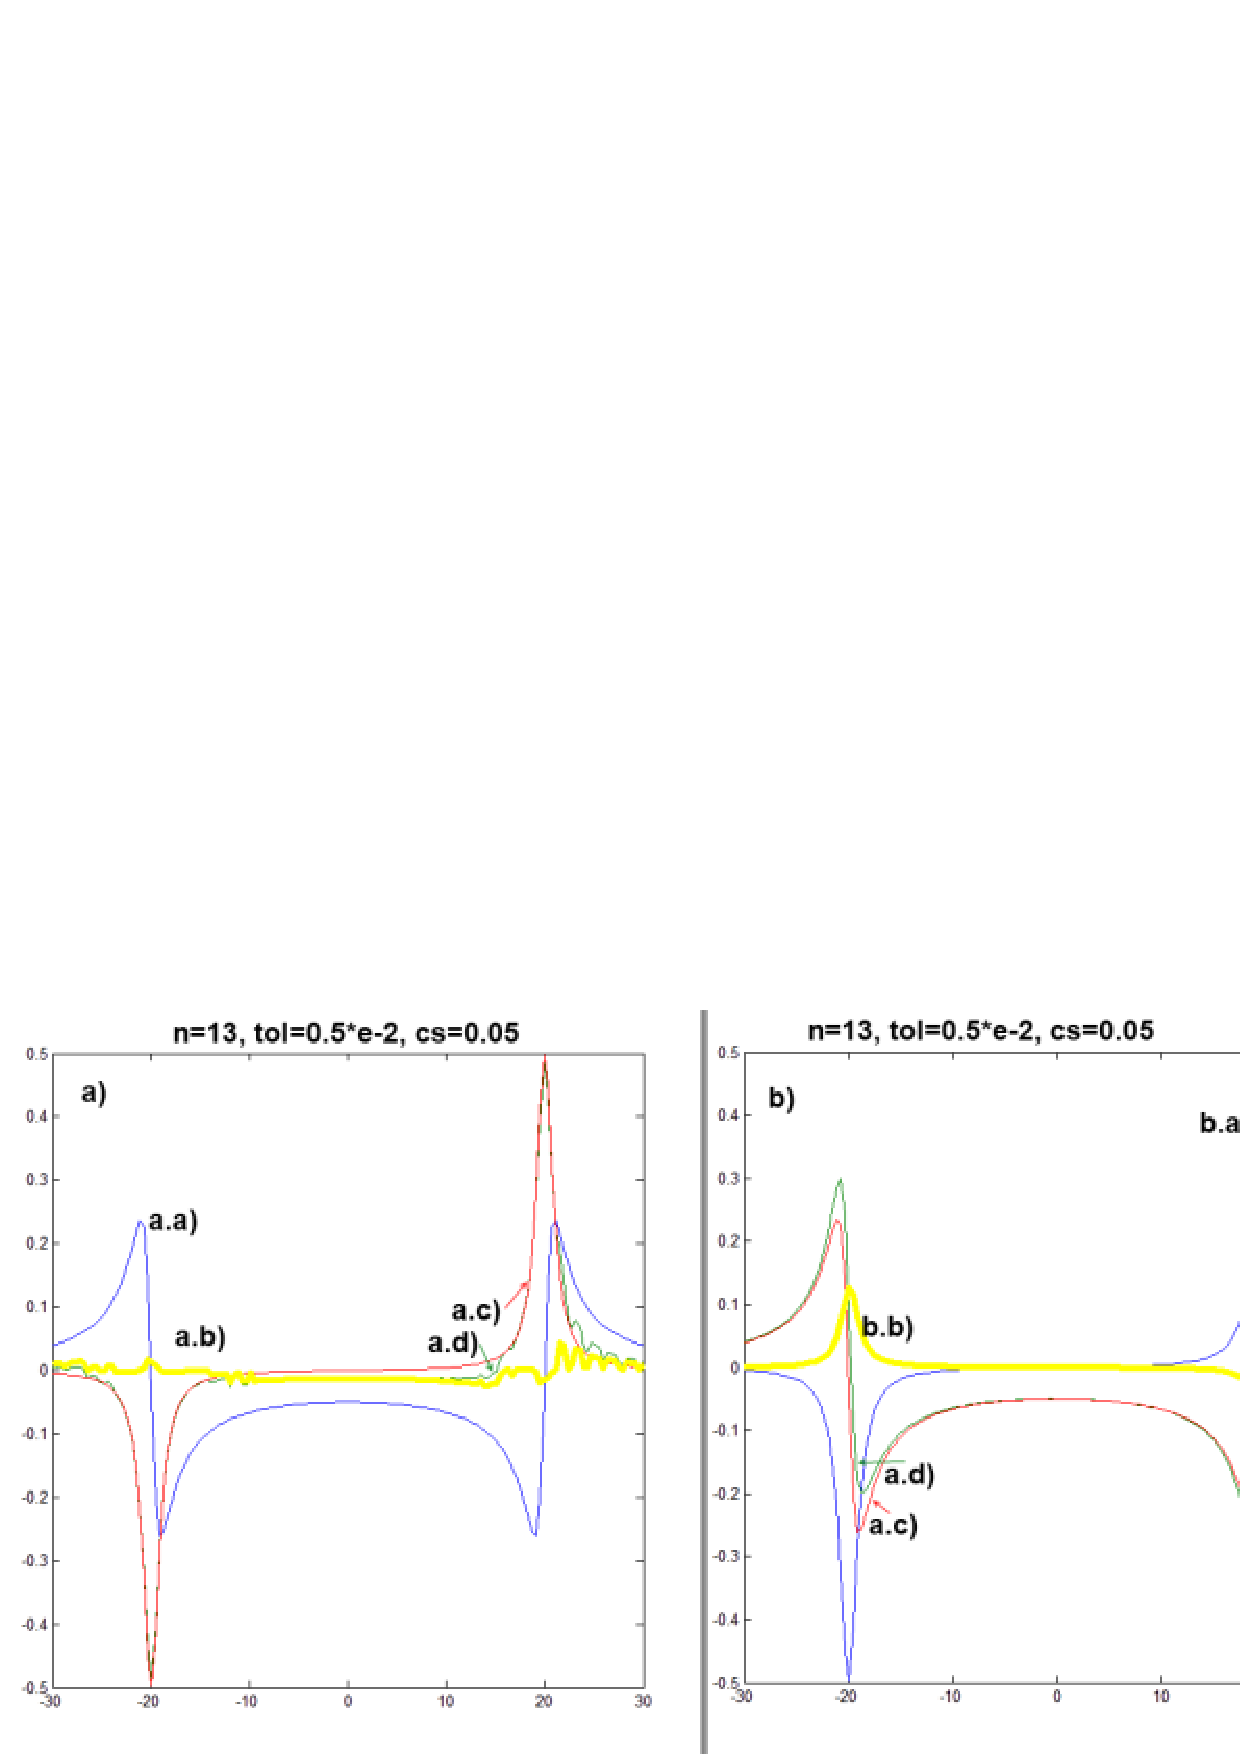
\includegraphics[width=150mm]{img/nc_lin3.png}
  \caption{ The Figure presents the third of four results of the NC Hilbert Transform method applied for the simple linear model. Results
   are plotted together. Calculations were performed with the parameters ($n = 13, \ , tol = \mbox{.5e-2}, \, c_s = \mbox{.5e-1})$
    a.a) The plot of the real part of $\chi (\omega )$
    a.b) absolute error plot (a.d-plot minus a.c-plot) 
    a.c) imaginary part of $\chi (\omega )$ calculated analytically 
    a.d) imaginary part of $\chi (\omega )$ obtained with the NC Hilbert transform of a.a-plot, 
    b.a) The plot of the imaginary part of $\chi (\omega )$
    b.b) absolute error plot (b.d-plot minus b.c-plot) 
    b.c) real part of $\chi (\omega )$ calculated analytically 
    b.d) real part of $\chi (\omega )$ obtained with the NC Hilbert transform of b.a-plot
    \label{fig:nc_lin3}     
  }
\end{figure}

\begin{figure}
  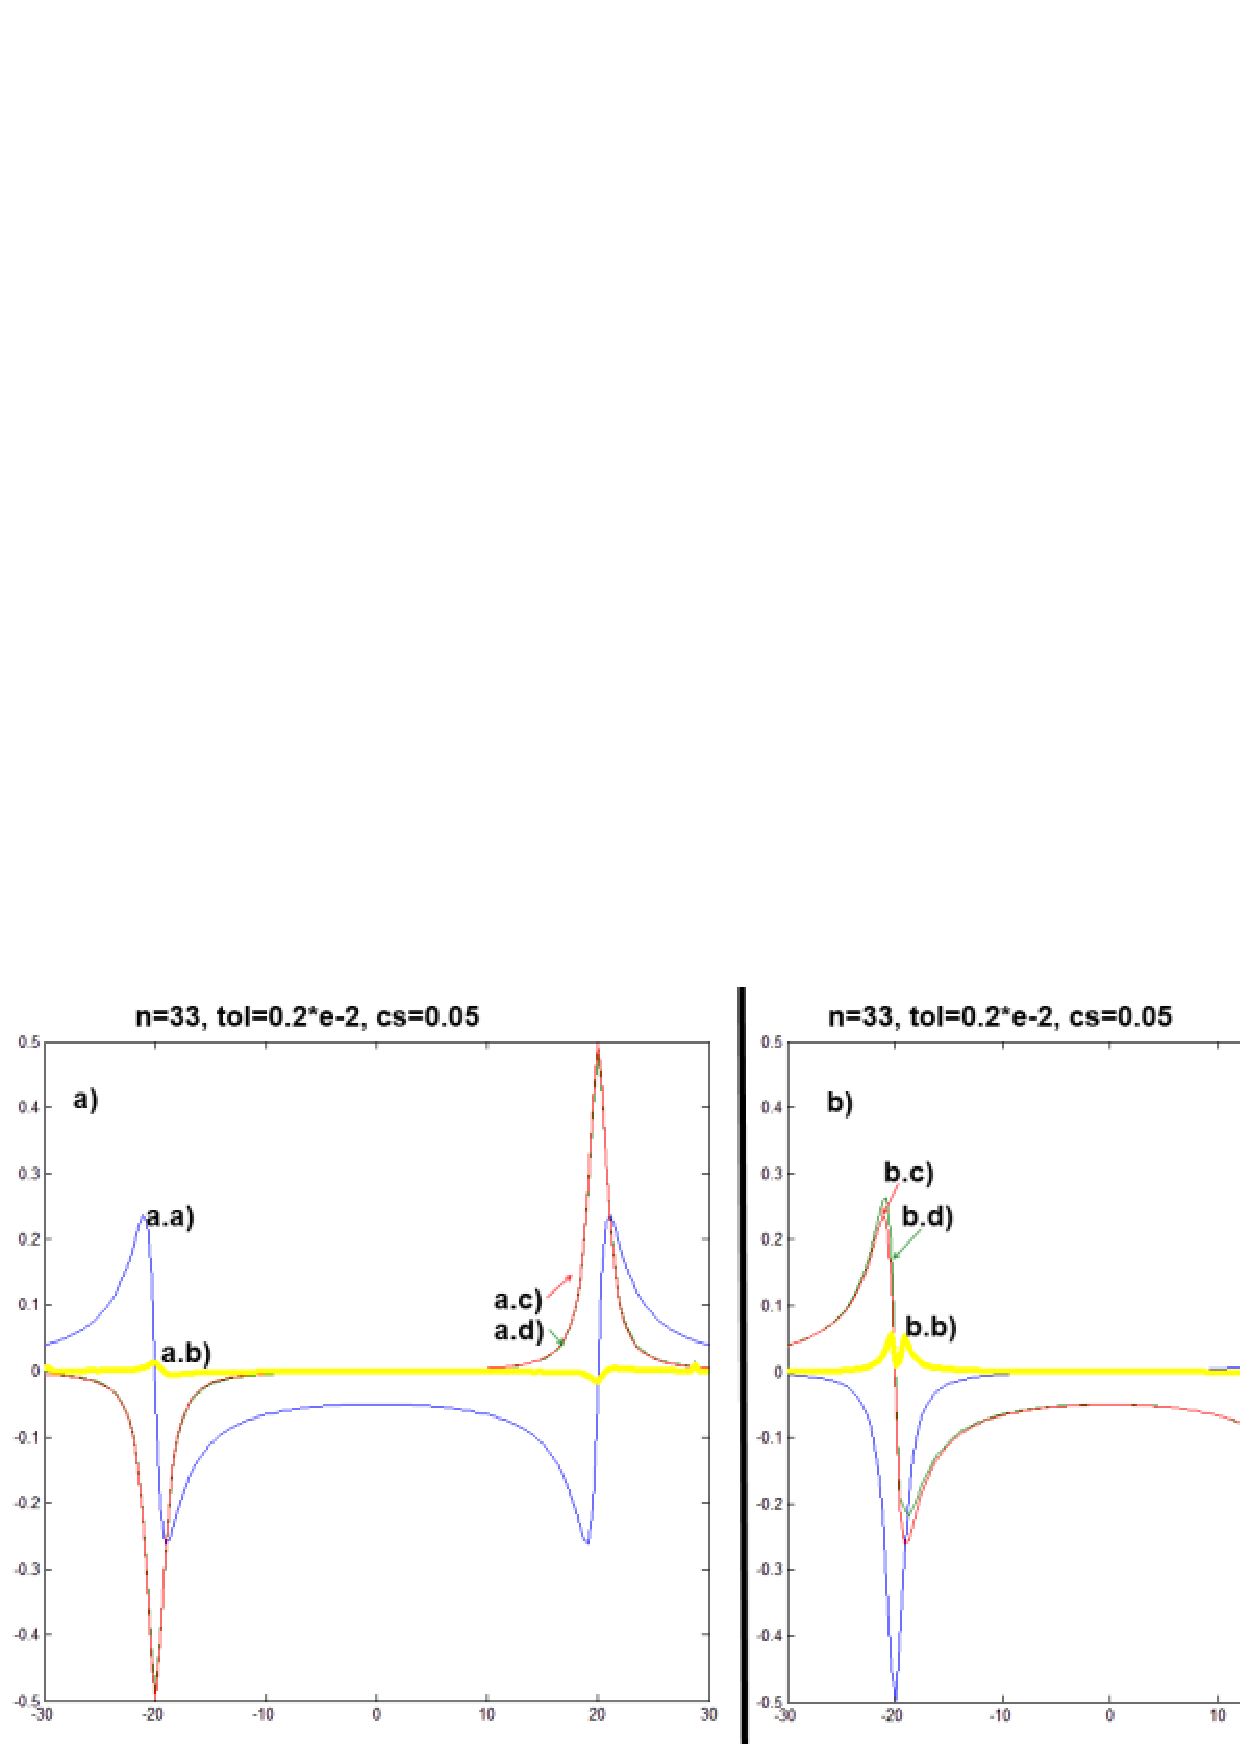
\includegraphics[width=150mm]{img/nc_lin4.png}
  \caption{The Figure presents the fourth of four results of the NC Hilbert Transform method applied for the simple linear model. Results
   are plotted together. Calculations were performed with the parameters ($n = 33, \, tol = \mbox{.2e-2}, \, c_s = \mbox{.5e-1}) $
    a.a) The plot of the real part of $\chi (\omega )$
    a.b) absolute error plot (a.d-plot minus a.c-plot) 
    a.c) imaginary part of $\chi (\omega )$ calculated analytically 
    a.d) imaginary part of $\chi (\omega )$ obtained with the NC Hilbert transform of a.a-plot,
    b.a) The plot of the imaginary part of $\chi (\omega )$
    b.b) absolute error plot (b.d-plot minus b.c-plot) 
    b.c) real part of $\chi (\omega )$ calculated analytically 
    b.d) real part of $\chi (\omega )$ obtained with the NC Hilbert transform of b.a-plot
    \label{fig:nc_lin4} 
    }
\end{figure}

We cannot tell with a hundred percent confidence which set of parameters will fit the best any given function and the user will
need to try many combinations before obtaining the final plot, but what we gave is the opportunity to set each one parameter manually,
which may lead to better results in the particular cases.

\subsection{NC for simple nonlinear model - results} \label{chap:nc_nlo}

We have performed calculations for the same both nonlinear pump-probe (\ref{eq:htran_fparameters}) and wave-mixing (\ref{eq:htran_feffexp})
models as in the Chapter (\ref{chap:htran_lin}) with the same set of parameters (constant values).

Results for pump-and-probe model has been presented in Figure (\ref{fig:nc_pnp}). Results for the frequency mixing model has been
presented in Figure (\ref{fig:nc_fmix1}). 

\begin{figure} 
  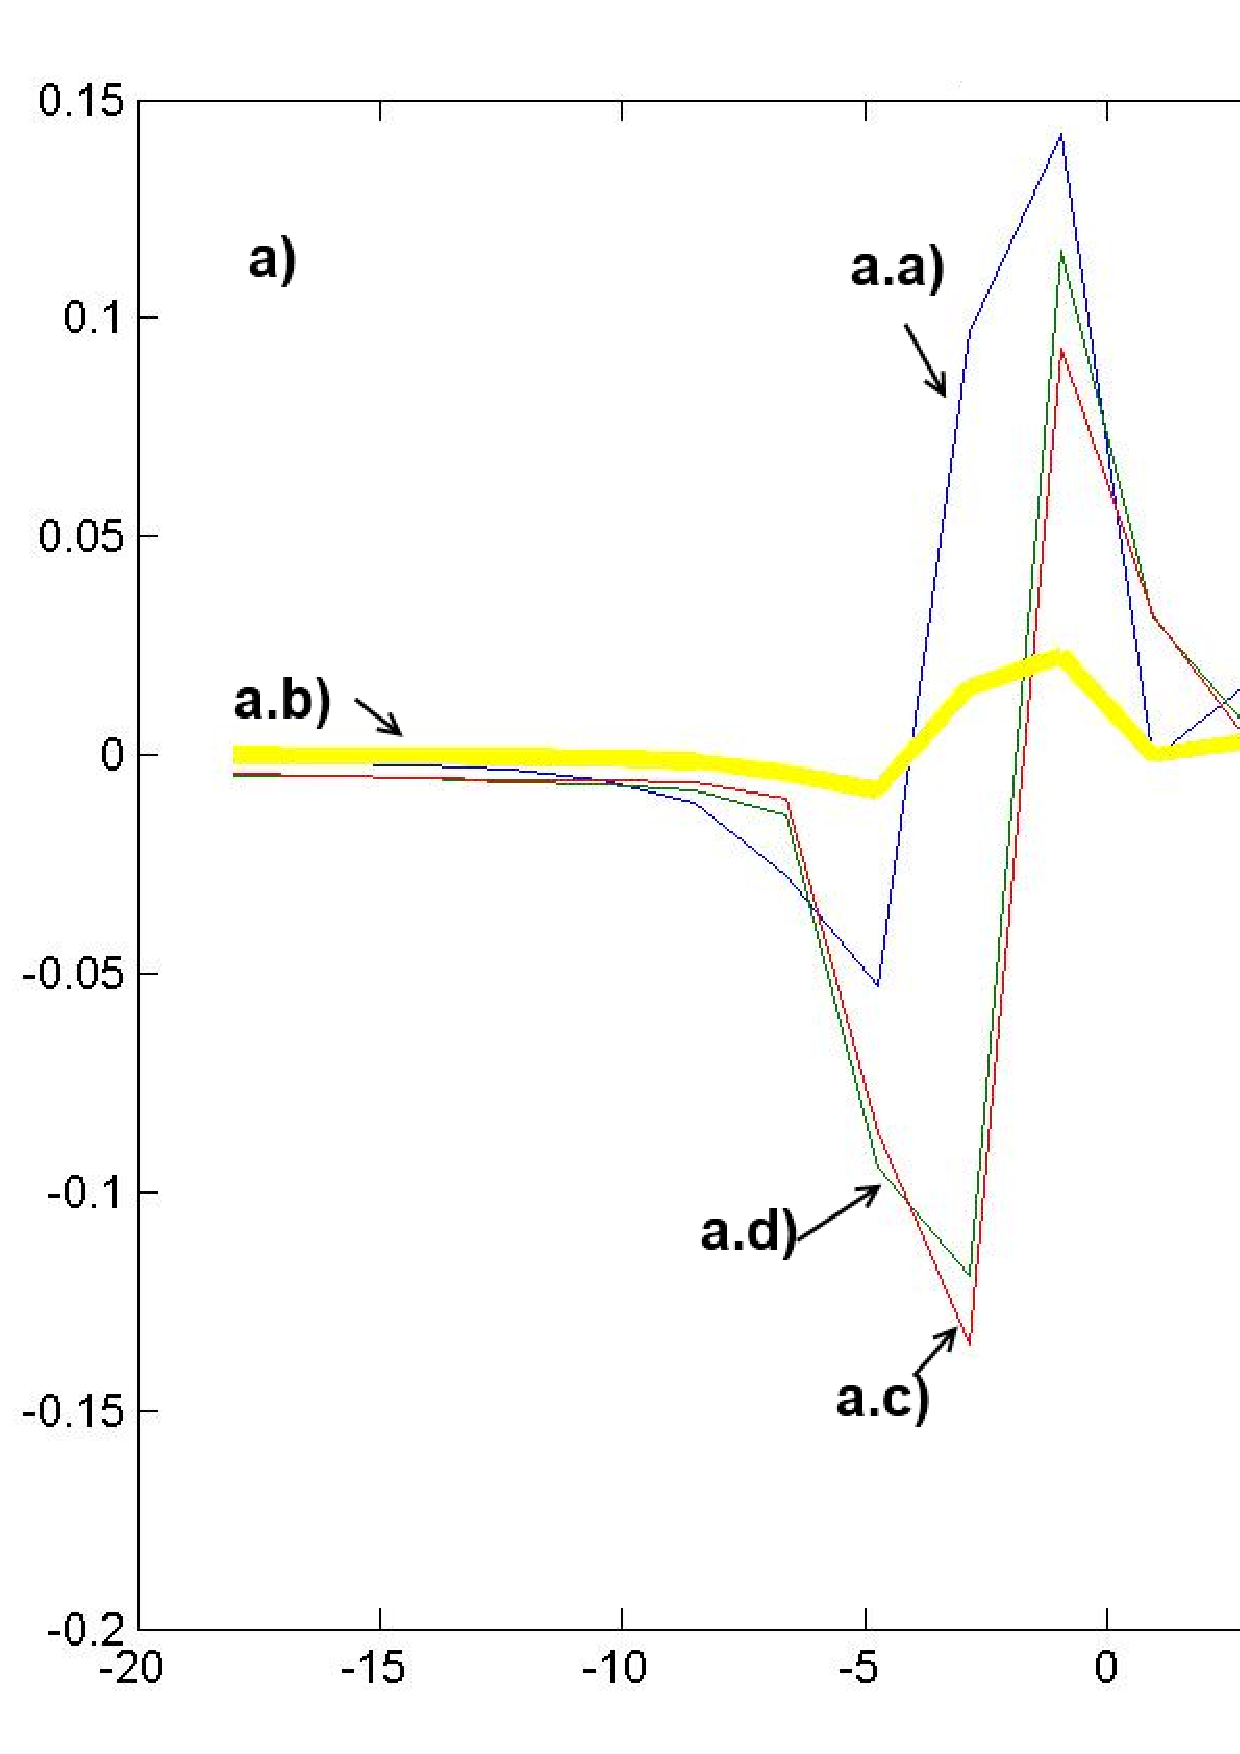
\includegraphics[width=150mm]{img/nc_pnp.png}
  \caption{ The Figure presents results of the NC Hilbert Transform method applied for the pump-and-probe model. Results
   are plotted together. Calculations were performed with the parameters ($n = 4, \, c_s = \mbox{.1e-1}, \, tol = \mbox{.1e-1})$
     a.a) The plot of the real part of ${\chi_{pp}}(\omega )$
     a.b) absolute error plot (a.d-plot minus a.c-plot) 
     a.c) imaginary part of ${\chi_{pp}}(\omega )$ calculated analytically 
     a.d) imaginary part of ${\chi_{pp}}(\omega )$ obtained with the NC Hilbert transform of a.a-plot, 
     b.a) The plot of the imaginary part of ${\chi_{pp}}(\omega )$ 
     b.b) absolute error plot (b.d-plot minus b.c-plot) 
     b.c) real part of $\chi_{pp} (\omega )$ calculated analytically 
     b.d) real part of ${\chi_{pp}}(\omega )$ obtained with the NC Hilbert transform of b.a-plot.
     With so few points and relatively long execution time the HNC method seems to be not a best fit for the analysis. We can see only the
     first sketch of calculated plot and based on that result we can initially falsify the investigated model. In this case the model seems
     to be correct.
     \label{fig:nc_pnp}
     }
\end{figure} 

\begin{figure} 
  \includegraphics[width=150mm]{img/nc_fmix1.png}
  \caption{ The Figure presents results of the NC Hilbert Transform method applied for the frequency mixing model.
  Results are plotted together. Calculations were performed with the parameters ($n = 8, \, c_s = \mbox{.3e-2}, \, tol = \mbox{.1e-1})$
     a.a) The plot of the real part of ${\chi_{mix}}(\omega )$
     a.b) absolute error plot (a.d-plot minus a.c-plot) 
     a.c) imaginary part of ${\chi_{mix}}(\omega )$ calculated analytically 
     a.d) imaginary part of ${\chi_{mix}}(\omega )$ obtained with the Hilbert transform of a.a-plot, 
     b.a) The plot of the imaginary part of ${\chi_{mix}}(\omega )$ 
     b.b) absolute error plot (b.d-plot minus b.c-plot) 
     b.c) real part of $\chi_{mix} (\omega )$ calculated analytically 
     b.d) real part of ${\chi_{mix}}(\omega )$ obtained with the Hilbert transform of b.a-plot
     We managed to use more points than in Figure (\ref{fig:nc_pnp}). We have received quite low error, but still in some areas 
     the method seems to generate large error.
     \label{fig:nc_fmix1}
     }
\end{figure}

\subsection{NC for simple quantum-perturbative model - results} \label{chap:nc_quantum}

\subsubsection*{Linear model - results:}

For the linear susceptibility we have used the model from Chapter (\ref{chap:problem_quantum}): 

\begin{equation} \label{eq:nclin_chipp}
  \chi_{1, \, qp}(\omega ) = \frac {N}{\varepsilon_0 \, h} \sum_{n=1}^{2} \, 
    ( \frac {{\mu_{1, \,n}} \, { \mu_{2, \, n}}}
            {{\Omega_{n}} - \omega  - i \, {\gamma_{n}}} 
    + \frac {{\mu_{2, \,n}}\,{\mu_{1, \,n}}}
            {{\Omega_{n}} + \omega + i \, {\gamma_{n}}} )
\end{equation}

This time we used the following parameters: 

\begin{equation}
  \mu = \begin{bmatrix} 
    3, & - 0.5 \\ 1.2, & 2.4
  \end{bmatrix},
  \Omega = \begin{bmatrix} 
    - 3, & 13
  \end{bmatrix}, \,
  \gamma = \begin{bmatrix} 
    0.7, & 2.3
  \end{bmatrix}, \,
  N = 8, \,
  \varepsilon_{0} = 1.4, \,
  h = - 2.7.
\end{equation} 

Evaluation time of two plots given in Figure (\ref{fig:nc_qp1}) was 615 seconds.

\begin{figure}
  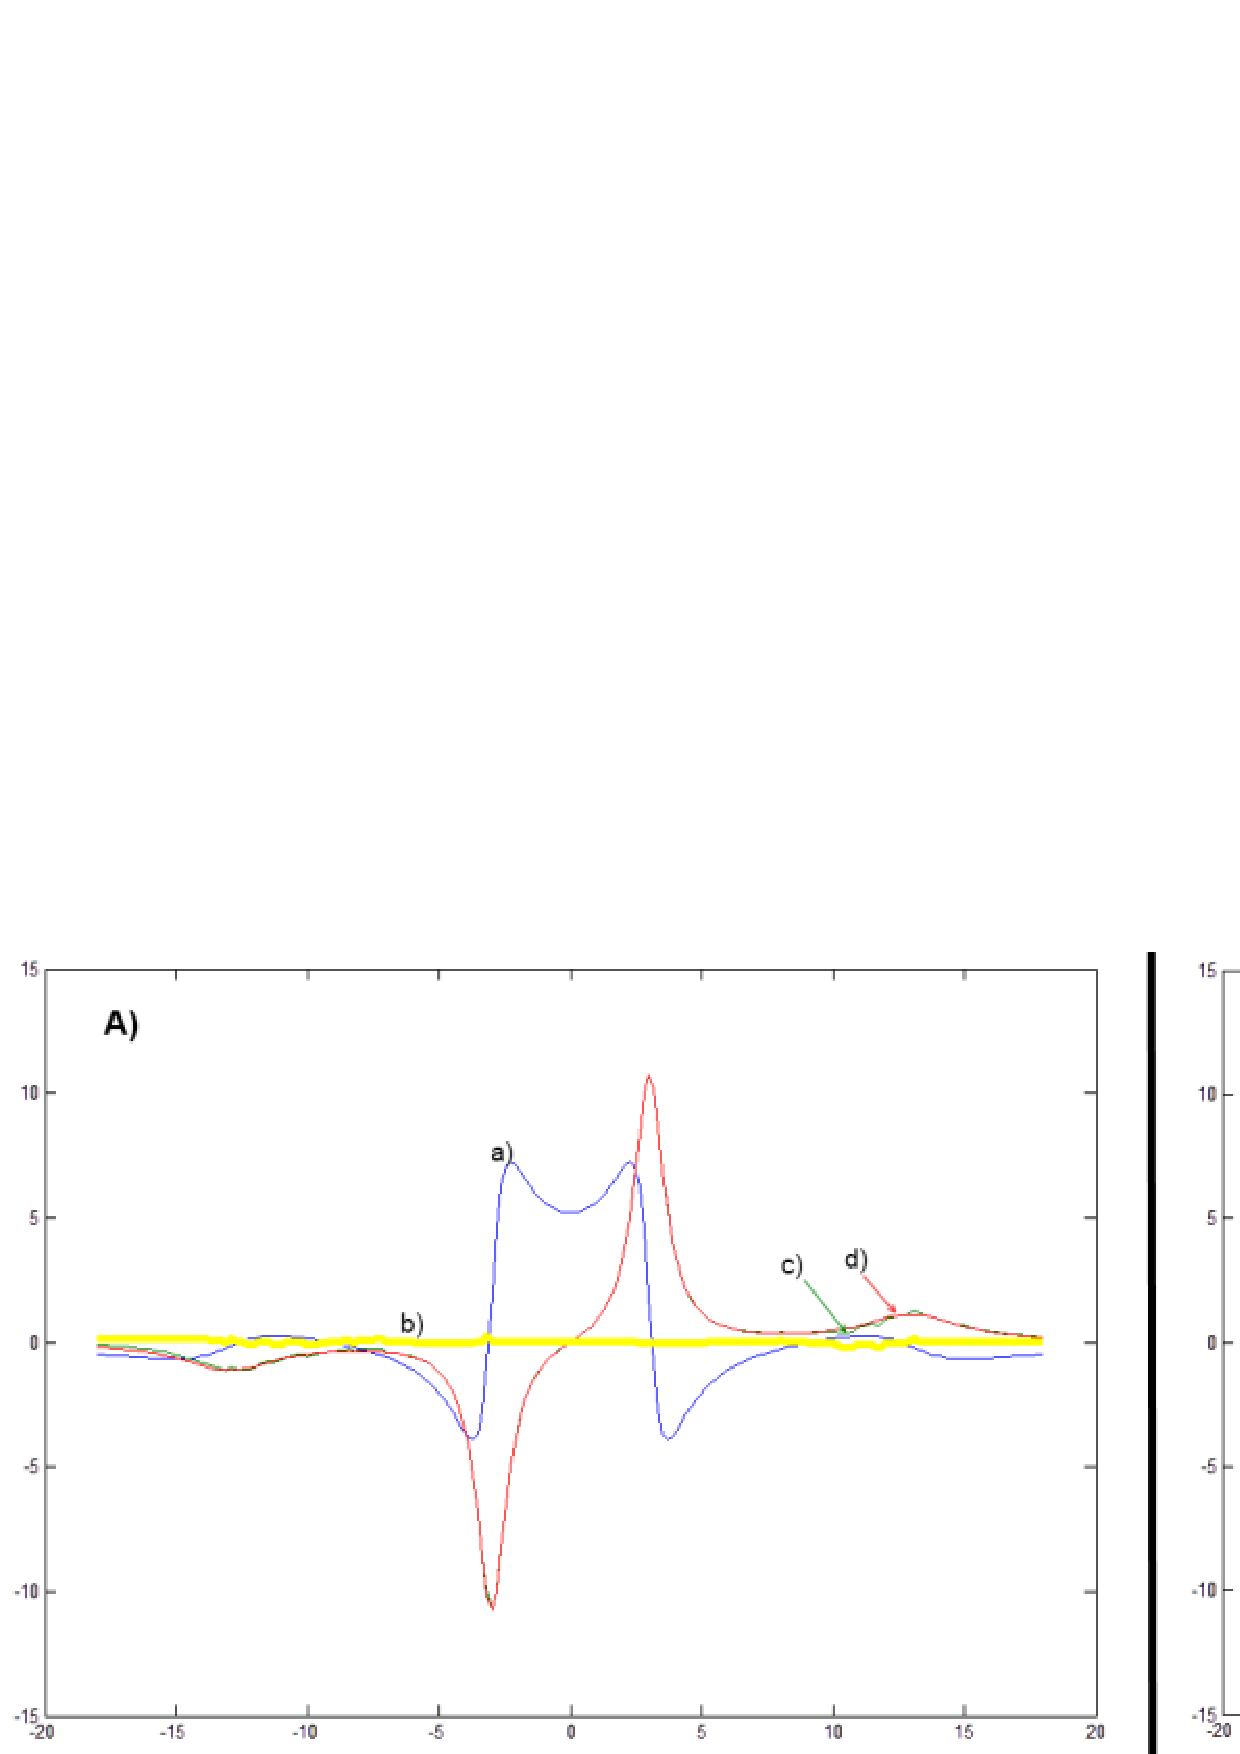
\includegraphics[width=150mm]{img/nc_qp1.png}
  \caption{ The Figure presents results of the NC Hilbert Transform method applied for the simple quantum-perturbative
  model. Results are plotted together. 
    a.a) The plot of the imaginary part of ${\chi_{1, \, qp}}(\omega )$
    a.b) absolute error plot (d-plot minus c-plot) 
    a.c) real part of ${\chi_{1, \, qp}}(\omega )$ obtained with the NC Hilbert transform of a-plot 
    a.d) real part of ${\chi_{1, \, qp}}(\omega )$ calculated analytically 
    b.b) The plot of the real part of ${\chi_{1, \, qp}}(\omega )$ 
    b.b) absolute error plot (d-plot minus c-plot) 
    b.c) imaginary part of ${\chi_{1, \, qp}}(\omega )$ obtained with the NC Hilbert transform of a-plot 
    b.d) imaginary part of ${\chi_{1, \, qp}}(\omega )$ calculated analytically
    We can see a good fit, but still in some areas results are with high error.  
    \label{fig:nc_qp1}
  }
\end{figure}

\subsubsection*{Second-order model - results:}

For the second-order susceptibility we used the model from Chapter (\ref{chap:problem_quantum}):

\begin{equation}  \label{eq:nclin_chipp2}
  \begin{split} 
     & \chi_{2, \, qp}(\omega_1, \, \omega_2 ) = 
    \frac{N} {2 \, \varepsilon_0 \, h^2} \sum_{n=1}^{2} \sum_{m=1}^{2} \sum_{l=1}^{2} 
    \\ ( & \frac {{\mu_{ln}} \, {\mu_{nm}} \, {\mu_{ml}} \, ({\Omega_{ml}} - \omega_1 - i \, {\gamma_{ml}})^{-1} }
        {({\Omega_{nl}} - \omega_1 - \omega_2 - i \, {\gamma_{nl}}) }
       + \frac {{\mu_{ln}} \, {\mu_{nm}} \, {\mu_{ml}} \, ({\Omega_{ml}} - \omega_2 - i \, {\gamma_{ml}})^{-1} }
        {({\Omega_{nl}} - \omega_1 - \omega_1 - i \, {\gamma_{nl}}) } 
    \\ + & \frac {{\mu_{ln}} \, {\mu_{nm}} \, {\mu_{ml}} \, ({\Omega_{nl}} + \omega_2 + i \, {\gamma_{nl}})^{-1} }
        {({\Omega_{mn}} - \omega_1 - \omega_2 - i \, {\gamma_{mn}}) } 
       + \frac {{\mu_{ln}} \, {\mu_{nm}} \, {\mu_{ml}} \, ({\Omega_{nl}} + \omega_2 + i \, {\gamma_{nl}})^{-1} }
        {({\Omega_{mn}} - \omega_1 - \omega_2 - i \, {\gamma_{mn}}) } 
    \\ + & \frac {{\mu_{ln}} \, {\mu_{nm}} \, {\mu_{ml}} \, ({\Omega_{ml}} - \omega_1 - i \, {\gamma_{ml}})^{-1} }
        {({\Omega_{nm}} + \omega_1 + \omega_2 + i \, {\gamma_{nm}}) } 
       + \frac {{\mu_{ln}} \, {\mu_{nm}} \, {\mu_{ml}} \, ({\Omega_{ml}} - \omega_1 - i \, {\gamma_{ml}})^{-1} }
        {({\Omega_{nm}} + \omega_1 + \omega_2 + i \, {\gamma_{nm}}) } 
    \\ + & \frac {{\mu_{ln}} \, {\mu_{nm}} \, {\mu_{ml}} \, ({\Omega_{nl}} + \omega_1 + i \, {\gamma_{nl}})^{-1} }
        {({\Omega_{ml}} + \omega_1 + \omega_2 + i \, {\gamma_{ml}}) } 
       + \frac {{\mu_{ln}} \, {\mu_{nm}} \, {\mu_{ml}} \, ({\Omega_{nl}} + \omega_2 + i \, {\gamma_{nl}})^{-1} }
        {({\Omega_{ml}} + \omega_1 + \omega_2 + i \, {\gamma_{ml}})}).
  \end{split} 
\end{equation}

with the constant values already chosen:

\begin{equation} \label{eq:nclin_const2}
  \mu = \begin{bmatrix} 
    1, & 3 \\ -1, & -2 
  \end{bmatrix} \, 
  \Omega = \begin{bmatrix} 
    3, & 16 \\ 4, & 12 
  \end{bmatrix} \,
  \gamma = \begin{bmatrix} 
  1, & 2 \\ -1, & 3
  \end{bmatrix} \, 
  N = 5, \, 
  \varepsilon_0 = 1, \,
  h= - 1.
\end{equation}

Results are presented in Figure (\ref{fig:nc_quantum2}). We can see a very large relative error reaching up to the 100\%. We may also
suspect this model is invalid. This will be checked with another methods in next chapters.

\begin{figure} 
  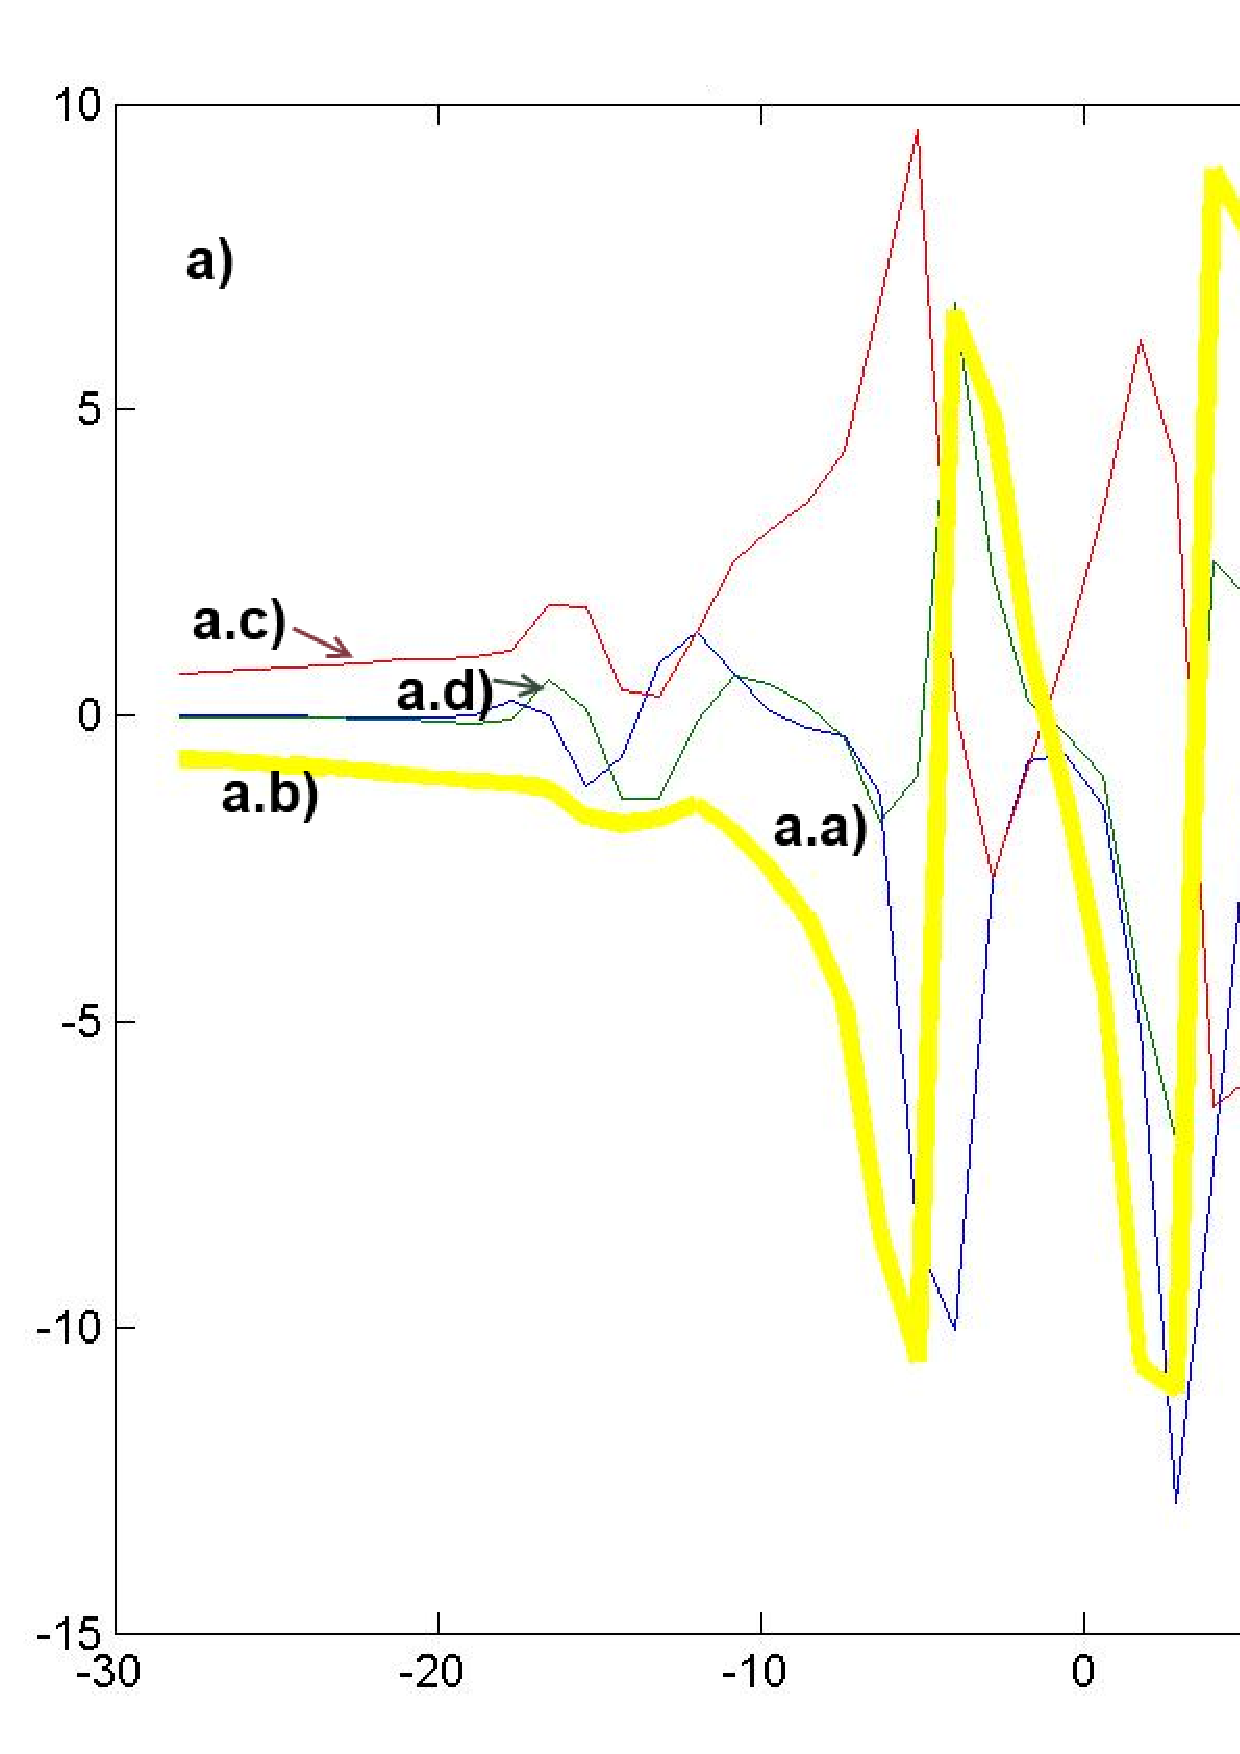
\includegraphics[width=150mm]{img/nc_quantum2.png}
  \caption{The Figure presents the results of the NC Hilbert Transform method applied for the second-order
  quantum-perturbative model. Results are plotted together. Calculations were performed with the parameters ($n = 4, \, c_s = \mbox{.1e-1}),
  \,tol=\mbox{.1e-1}$ a.a) The plot of the real part of ${\chi_{2, \,qp}}(\omega )$
     a.b) absolute error plot (a.d-plot minus a.c-plot) 
     a.c) imaginary part of ${\chi_{2, \,qp}}(\omega )$ calculated analytically 
     a.d) imaginary part of ${\chi_{2, \,qp}}(\omega )$ obtained with the NC Hilbert transform of a.a-plot, 
     b.a) The plot of the imaginary part of ${\chi_{2, \,qp}}(\omega )$ 
     b.b) absolute error plot (b.d-plot minus b.c-plot) 
     b.c) real part of $\chi_{2, \, qp} (\omega )$ calculated analytically 
     b.d) real part of $\chi_{2, \, qp} (\omega )$ obtained with the NC Hilbert transform of b.a-plot 
     \label{fig:nc_quantum2}
     }
\end{figure}
 
\section{Clenshaw-Curtis based Hilbert transform} \label{chap:hcc}

\subsection{Overview of the Clenshaw-Curtis based Hilbert transform implementation} \label{chap:hcc_overview}

The algorithm for the Hilbert transform using the modified Clenshaw-Curtis quadrature is presented. 

\subsubsection*{Clenshaw Curtis quadrature: }

The heart of the calculation has been presented by T. Hasegawa and T. Torri in \cite{Hasegawa1991}. First we will need to calculate
the Cauchy principal value integral on the interval $[-1, 1]$:

\begin{equation} \label{eq:hcc_cpvint}
	\dashint_{-1} ^ {1} \frac{f(x)} {(x-c)} \, d \, x \quad \text{for} \, c \in (-1, 1) .
\end{equation}


The first step suggested by the authors is to remove the singularity from the integral :

\begin{equation}   \label{eq:hcc_singularity}
  \dashint_{-1}^{1} \frac{f(x)}{(x-c)} d \, x = \dashint_{-1}^{1} \frac{f(x)-f(c)}{(x-c)} + f(c) \, log(\frac{1-c}{1+c})
\end{equation}

After some transformation authors finally obtain the iterative formula presented in equations (\ref{eq:hccformula_sum}) and
(\ref{eq:hccformula_rec}). The formula (\ref{eq:hccformula_sum}) depends on the parameter $N$, which will be used in the adaptive
algorithm. The recursive equation (\ref{eq:hccformula_rec}) should be solved with the starting values: $d_N = d_{N+1} = 0$

\begin{subequations} \label{eq:hcc_formula}
  \begin{equation}   \label{eq:hccformula_sum}
    \dashint_{-1}^{1} \frac{f(x)}{(x - c)} d \, x 
    \approx 2 \, \sideset{}{'} \sum_{k = 0} ^ {N / 2 - 1} \frac{d_{2k}}{1 - 4k ^ 2} + f(c) \, log(\frac{1-c} {1+c})
  \end{equation}
  \begin{equation}   \label{eq:hccformula_rec}
    d_{k+1} - 2 \, c \, d_k + d_{k-1} 
    = 2 \, a_k^N \, \text{ for } \, k = N, N - 1, \ldots , 1 .
  \end{equation}
\end{subequations}

The remaining issue is to calculate the coefficients $a_k ^ N$, that have been described in equation (\ref{eq:hcc_akn}).  $a_k ^ N$ is
also known as the discrete cosine transform of the first type (DCT-I):

\begin{equation} \label{eq:hcc_akn}
    a_k^N = \frac{2}{N} {\sideset{}{''}\sum_{j=0}^{N}} f\left(cos\left (\frac {\pi j}{N} \right)
    \right)\,cos\left(\frac{\pi k j}{N}\right), 0 \leq k \leq N
\end{equation}


\subsubsection*{Hilbert transform using the Clenshaw-Curtis quadrature:}

While the Clenshaw-Curtis quadrature is defined for finite range $[-1,\,1]$, the Hilbert transform is defined by the definite and improper
integral over the unbounded interval $[-\infty,\, \infty]$. Here we must remind the law of conservation of energy, from which we can easily
deduce that the susceptibility - as the investigated physical quantity - for low frequencies and thus for low energies has low
values. From this it follows that function $f = f(x)$ tends to zero when closing to infinities. Thereby the value of integrated
function from equation (\ref{eq:hcc_adapt}) decreases rapidly and for relatively large values of x this integrand will be omitted.

\begin{equation} \label{eq:hcc_adapt}
  \frac{f(x)}{x-c} d \, x
\end{equation}

Therefore, we will not be changing the integration range from interval to real line. What must be taken into consideration right
now is that the well-chosen, finite interval for integration stated in (\ref{eq:hcc_interval}) or an integral with an interval few times
bigger.

\begin{equation} \label{eq:hcc_interval}
  [A, B] = [a - 2|b-a|, b + 2|b-a|] 
\end{equation}

The specific choice of integration interval should be done during the numerical calculations. As default in our algorithm, we have
set the integration interval to be based on the (\ref{eq:hcc_interval}), but simply $5$ times longer. For all
investigated models it gave us satisfactory results.

\subsubsection*{Our implementation of the Hilbert Clenshaw-Curtis iterations:}

So far we have presented the overview of procedures responsible for evaluation of the Clenshaw-Curtis qua\-dra\-tu\-re and the Hil\-bert
transform using the Clenshaw-Curtis qua\-dra\-ture at one point. But in the typical situation we have the whole vector of function values
for a given range of abscissas - so what is left - we perform the single-point Hil\-bert transform based on the Clenshaw-Curtis
qua\-dra\-ture for each given point. But to omit the problems with singularities, we will add some post- and precalculations - using the cubic interpolation. The
whole procedure is now:


\textbf{INPUT:}
 

\begin{tabular}{ l l }

  $X$, $Y$ &- given $N$-length abscissas and related ordinates \\
  $A$, $B$ &- extended ranges of the interval (based on $Y$) \\
  
\end{tabular}


\emptyline


\textbf{PRE-CALCULATIONS:}

\begin{equation} \label{eq:cci_period}
  T = B - A
\end{equation}

\begin{equation} \label{eq:cci_center}
  C = \frac{B+A}{2}
\end{equation}

From $N$ points of $Y$ we calculate the cubic interpolation having $N-1$ inner points:

\begin{subequations} \label{eq:cci_cubicinterpolation}
  \begin{equation}   \label{eq:ccicinterp_first}
    {Yp_{1}}=\frac {3\,{Y_{1}} + 6\,{Y_{2}} - {Y_{3}}}{8}
  \end{equation}
  \begin{equation}   \label{eq:ccicinterp_next}
    {Yp_{k}}=\frac { - {Y_{k - 1}} + 9\,{Y_{k}} + 9\,{Y_{k + 1}} - {Y_{k + 2}}}{16}
  \end{equation}
  \begin{equation}   \label{eq:ccicinterp_last}
    {Yp_{N}}=\frac { - {Y_{N - 2}} + 6\,{Y_{N - 1}} + 3\,{Y_{N}}}{8}
  \end{equation}
\end{subequations}

\textbf{MAIN CALCULATIONS:}
As the central part, we calculate the $N-1$ values for each on of inner points: 

\begin{equation} \label{eq:cci_newd}
	d_k= \frac{2 \, (Yp_{k} - C ) }{T}, \text{ for k = 1, \ldots , \ $N-1$}
\end{equation}

\begin{equation} \label{eq:cci_approx}
  Hh_{k} \approx \frac{1}{\pi} \dashint_{A}^{B} \frac{f(\frac{x \, T}{2} + C)}{x-d_k} d\,x, \text{ for k = 1, \ldots , \ $N-1$}
\end{equation}

\textbf{POST-CALCULATIONS:} \\
From $N-1$ points of Hh we calculate $N$ points using the reverse cubic interpolation:

\begin{subequations} \label{eq:cci_revcubicinterp}
  \begin{equation}   \label{eq:ccircinterp_first}
    {H_{1}}=\frac {15\,{Hh_{1}} - 10\,{Hh_{2}} + 3\,{Hh_{3}}}{8}
  \end{equation}
  \begin{equation}   \label{eq:ccircinterp_second}
    {H_{2}}=\frac {3\,{Hh_{1}} + 6\,{Hh_{2}} - {Hh_{3}}}{8}
  \end{equation}
  \begin{equation}   \label{eq:ccircinterp_next}
    {H_{k}}=\frac { - {Hh_{k - 1}} + 9\,{Hh_{k}} + 9\,{Hh_{k + 1}} - {Hh_{k + 2}}}{16}
  \end{equation}
  \begin{equation}   \label{eq:ccircinterp_prelast}
    {H_{N - 1}}=\frac { - {Hh_{N - 3}} + 6\,{Hh_{2}} - {Hh_{3}}}{8}
  \end{equation}
  \begin{equation}   \label{eq:ccircinterp_last}
    {H_{N}}=\frac {3\,{Hh_{N - 3}} - 10\,{Hh_{N - 2}} + 15\,{Hh_{N - 1}}}{8}
  \end{equation}
\end{subequations}

\textbf{OUTPUT:} \\
\begin{tabular}{r l}
  H & - N-length Hilbert transform for given function values at X abscissas \\
\end{tabular}

\emptyline

The algorithm source has been presented in the Appendix A.3.

\subsection{HCCI for simple linear model} \label{chap:hcc_lin}

Figures (\ref{fig:cci_lin1}) and (\ref{fig:cci_lin2}) presents the results obtained with the method for the model defined in
model (\ref{eq:physical_frequency_linear}). As we can see - the Hilbert Clenshaw-Curtis iterations gives us much better accuracy than HTRAN
or Newton-Cotes quadrature. In next chapters we will check what happens for another models.

\begin{figure} 
  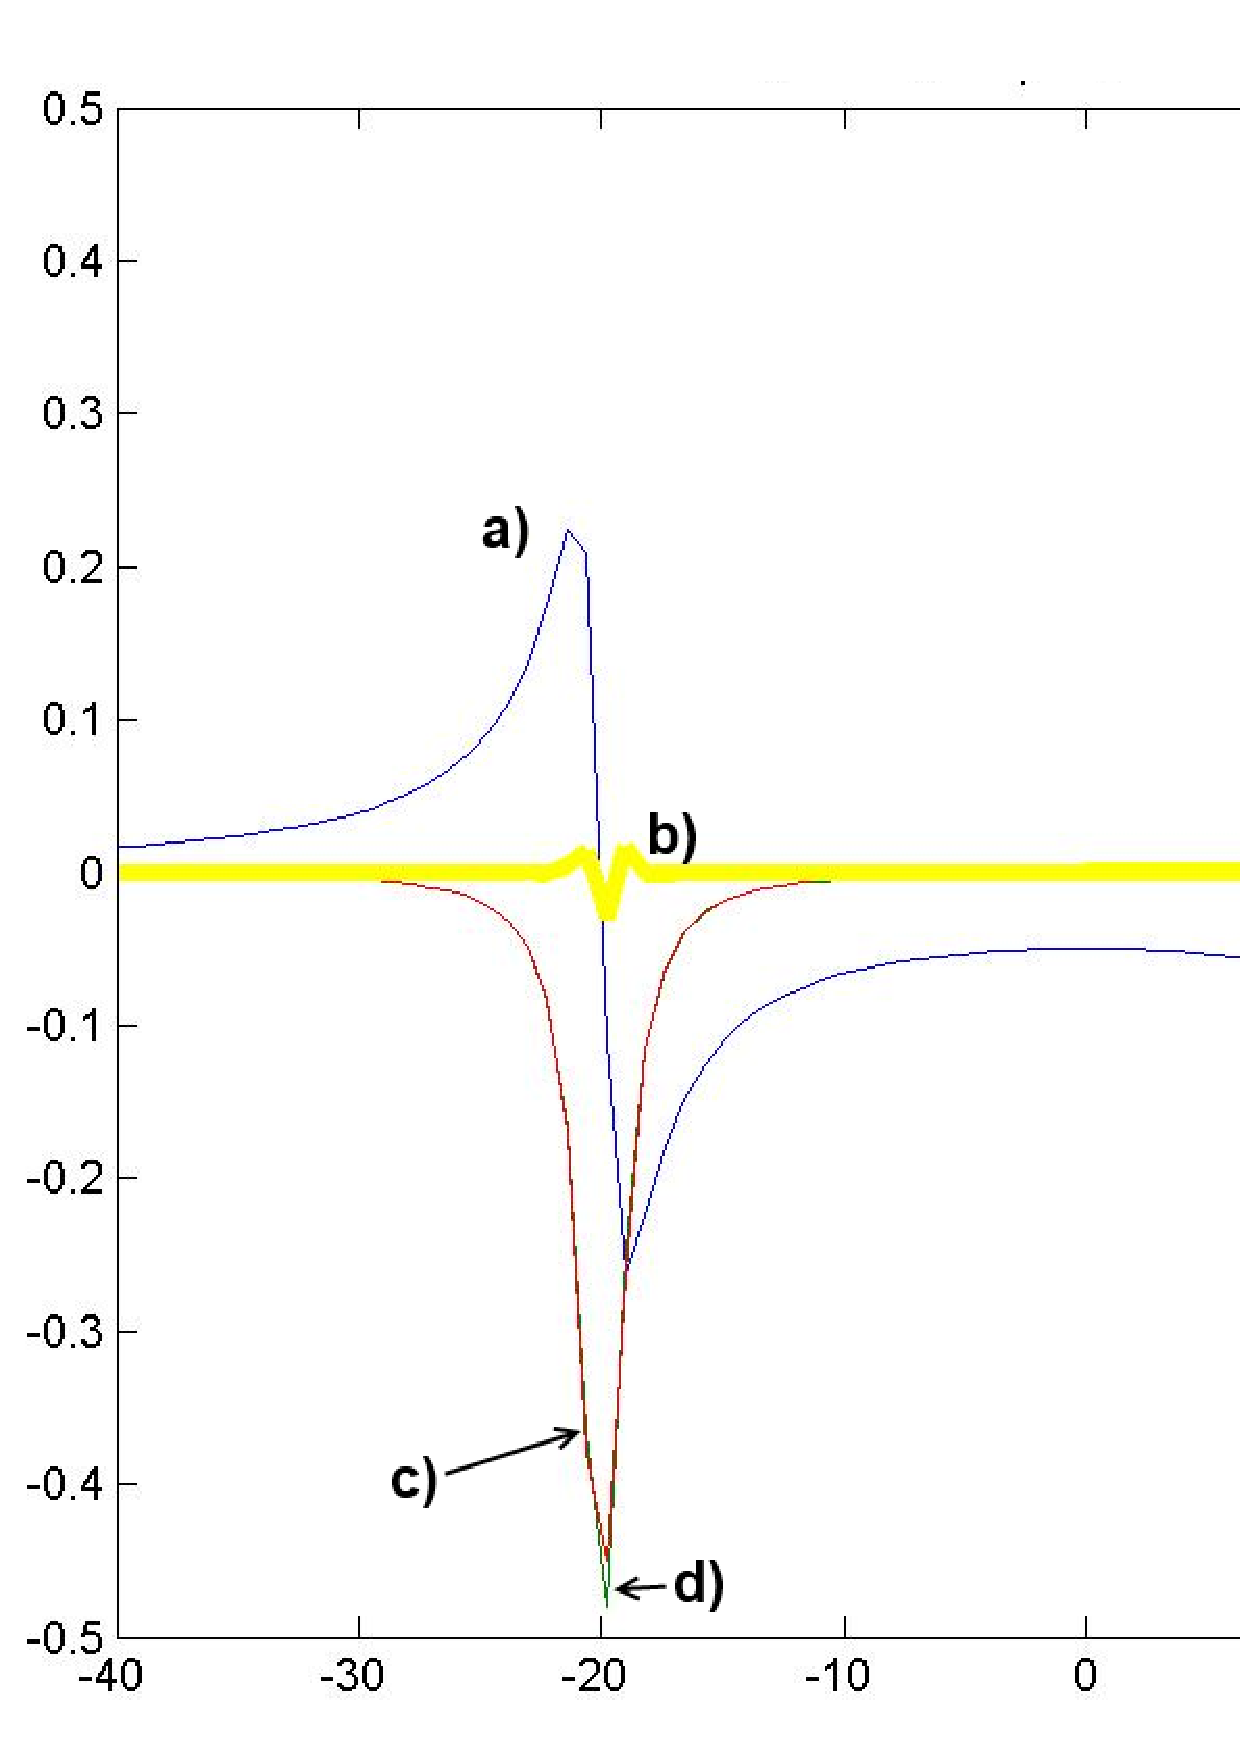
\includegraphics[width=150mm]{img/hcc_lin1.png}
  \caption{The Figure presents the results of the Hilbert Clenshaw-Curtis iterations method applied to the real part of the simple linear
  model. Results are plotted together.
   a) The plot of the real part of $\chi (\omega )$ 
   b) absolute error plot (c-plot minus d-plot) 
   c) imaginary part of $\chi (\omega )$ obtained with the Hilbert transform of a-plot 
   d) imaginary part of $\chi (\omega )$  calculated analytically. \label{fig:cci_lin1}
  }
\end{figure}

\begin{figure} 
  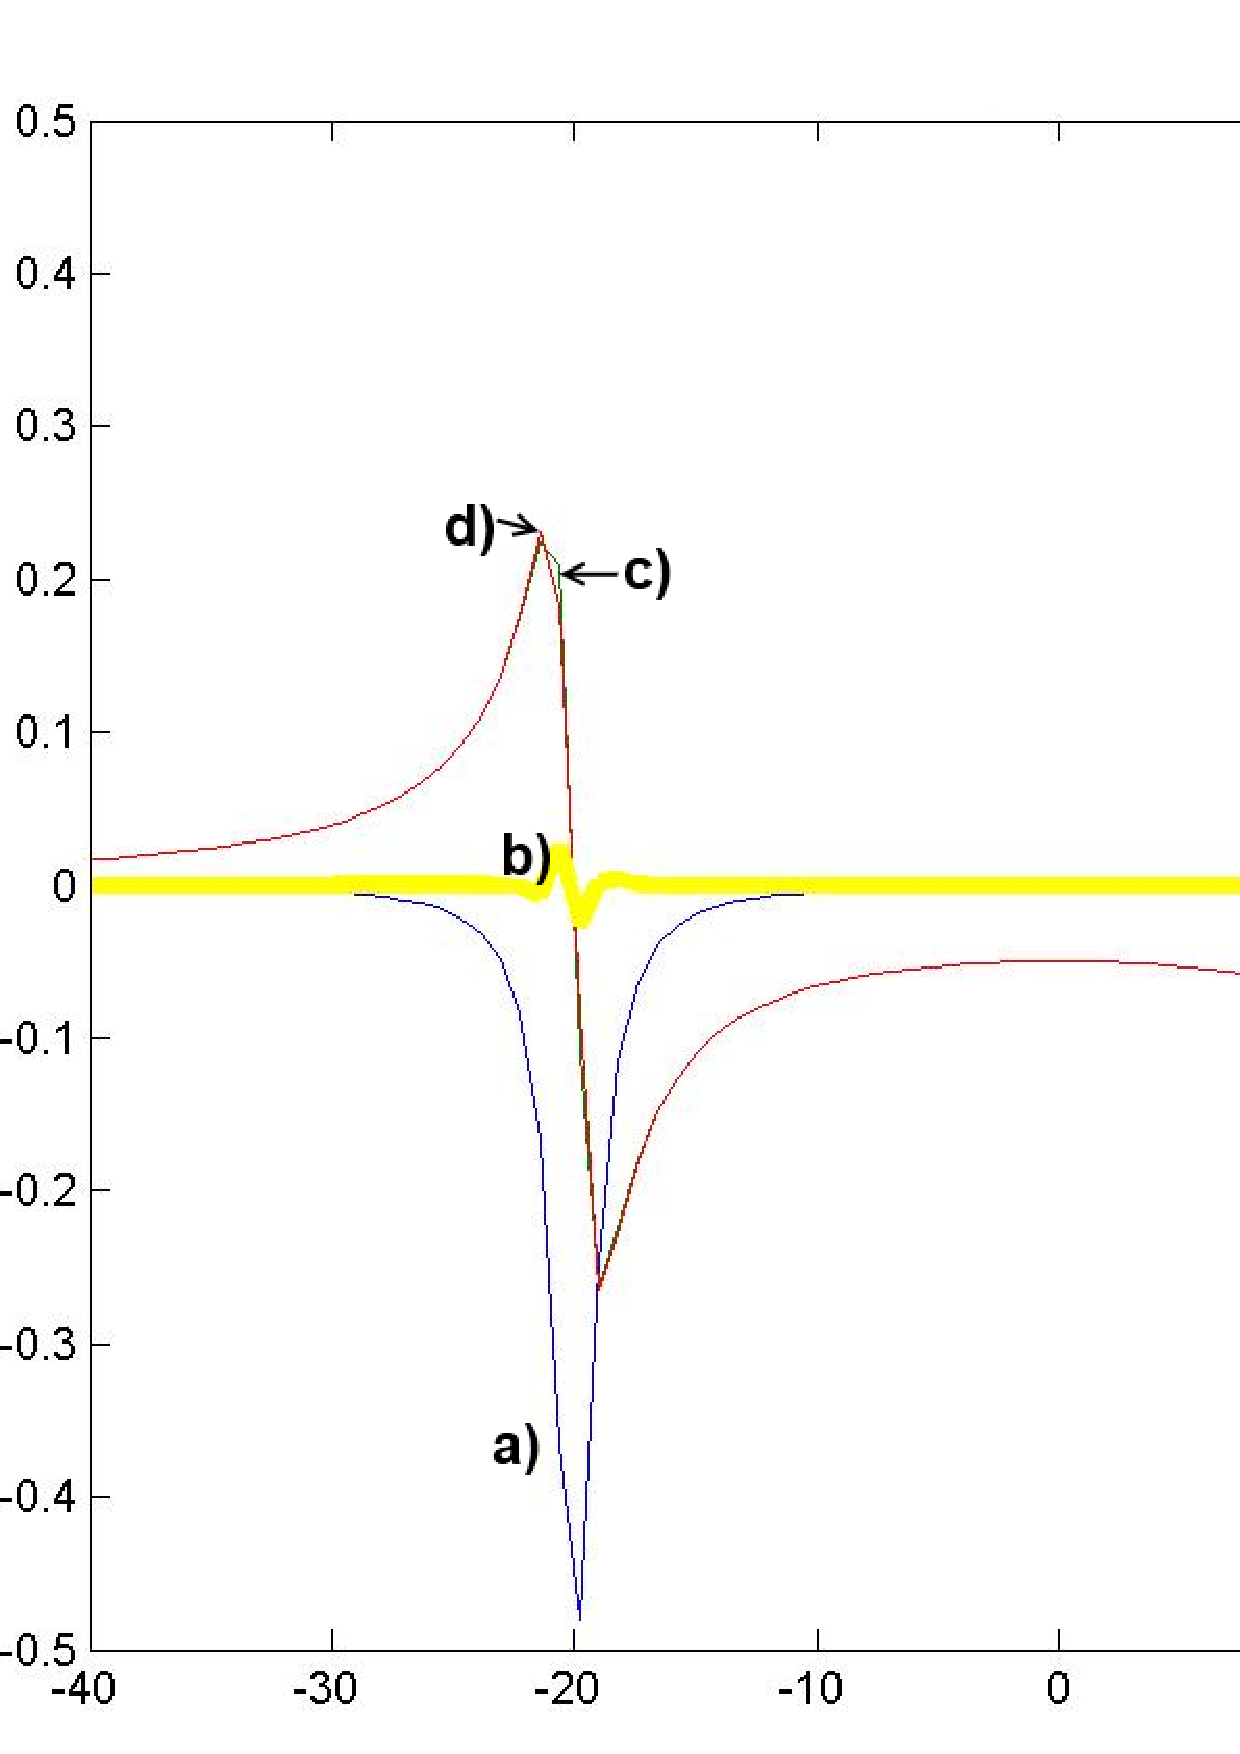
\includegraphics[width=150mm]{img/hcc_lin2.png}
  \caption{The Figure presents the results of the Hilbert Clenshaw-Curtis iterations method applied to the imaginary part of the simple
  linear model. Results are plotted together.
   a) The plot of the imaginary part of $\chi (\omega )$ 
   b) absolute error plot (c-plot minus d-plot) 
   c) real part of $\chi (\omega )$ obtained with the Hilbert transform of a-plot 
   d) real part of $\chi (\omega )$ calculated analytically. \label{fig:cci_lin2}
  }
\end{figure}

\subsection{HCCI for simple nonlinear model} \label{chap:hcc_nlo}

For the pump-probe and frequency mixing models we have used the same parameters as in Chapter (\ref{chap:nc_nlo}). The results
obtained with the Hilbert Clenshaw-Curtis iterations has been presented in Figures (\ref{fig:hcci_pnp}) and (\ref{fig:hcci_fmix})
respectively.

\begin{figure} 
  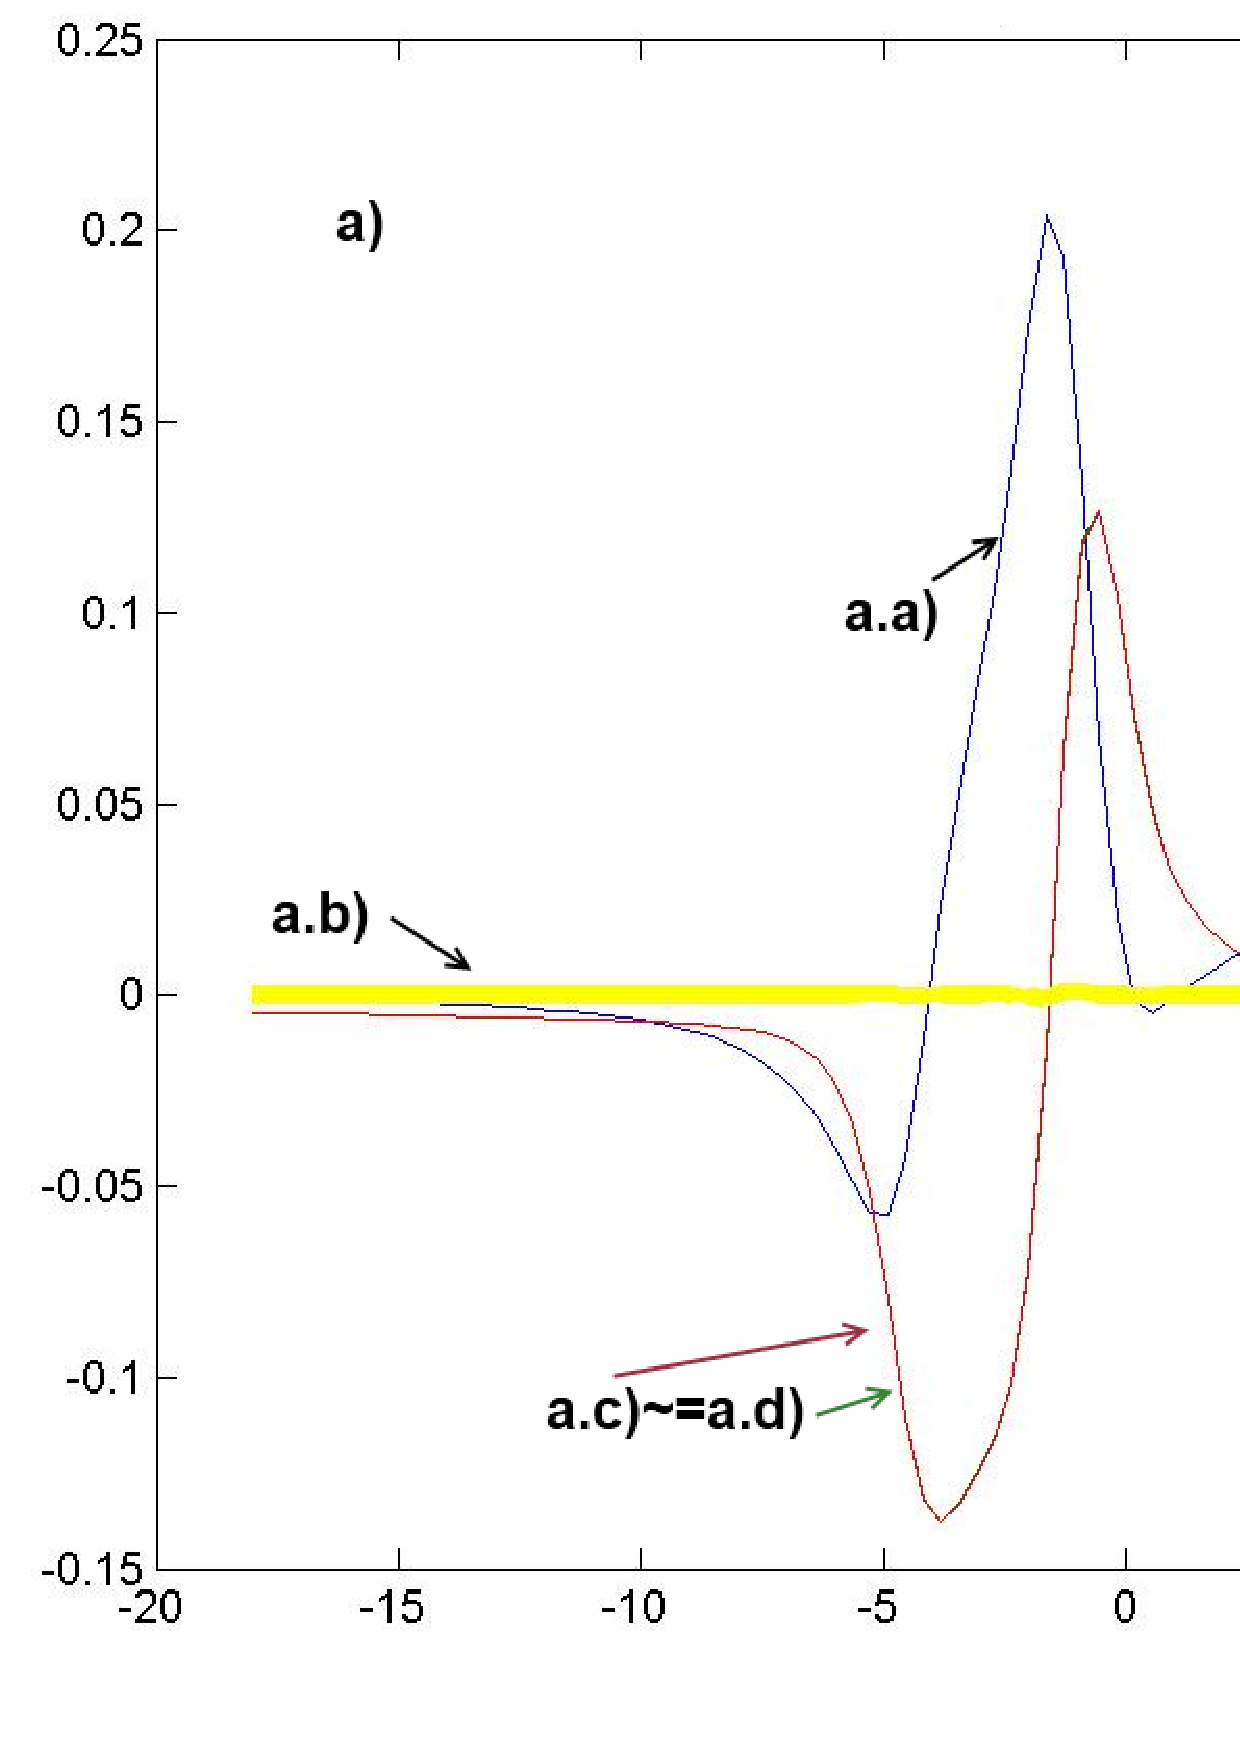
\includegraphics[width=150mm]{img/hcc_pnp.png}
  \caption{Results for the pump-probe model using the Hilbert Clenshaw-Curtis iterations
     a.a) The plot of the real part of ${\chi_{pp}}(\delta )$
     a.b) absolute error plot (a.d-plot minus a.c-plot) 
     a.c) imaginary part of ${\chi_{pp}}(\delta )$ calculated analytically 
     a.d) imaginary part of ${\chi_{pp}}(\delta )$ obtained with the Hilbert transform of a.a-plot, 
     b.a) The plot of the imaginary part of ${\chi_{pp}}(\delta )$ 
     b.b) absolute error plot (b.d-plot minus b.c-plot) 
     b.c) real part of $\chi_{pp} (\omega )$ calculated analytically 
     b.d) real part of ${\chi_{pp}}(\delta )$ obtained with the Hilbert transform of b.a-plot 
     \label{fig:hcci_pnp}
     }
\end{figure} 

\begin{figure} 
  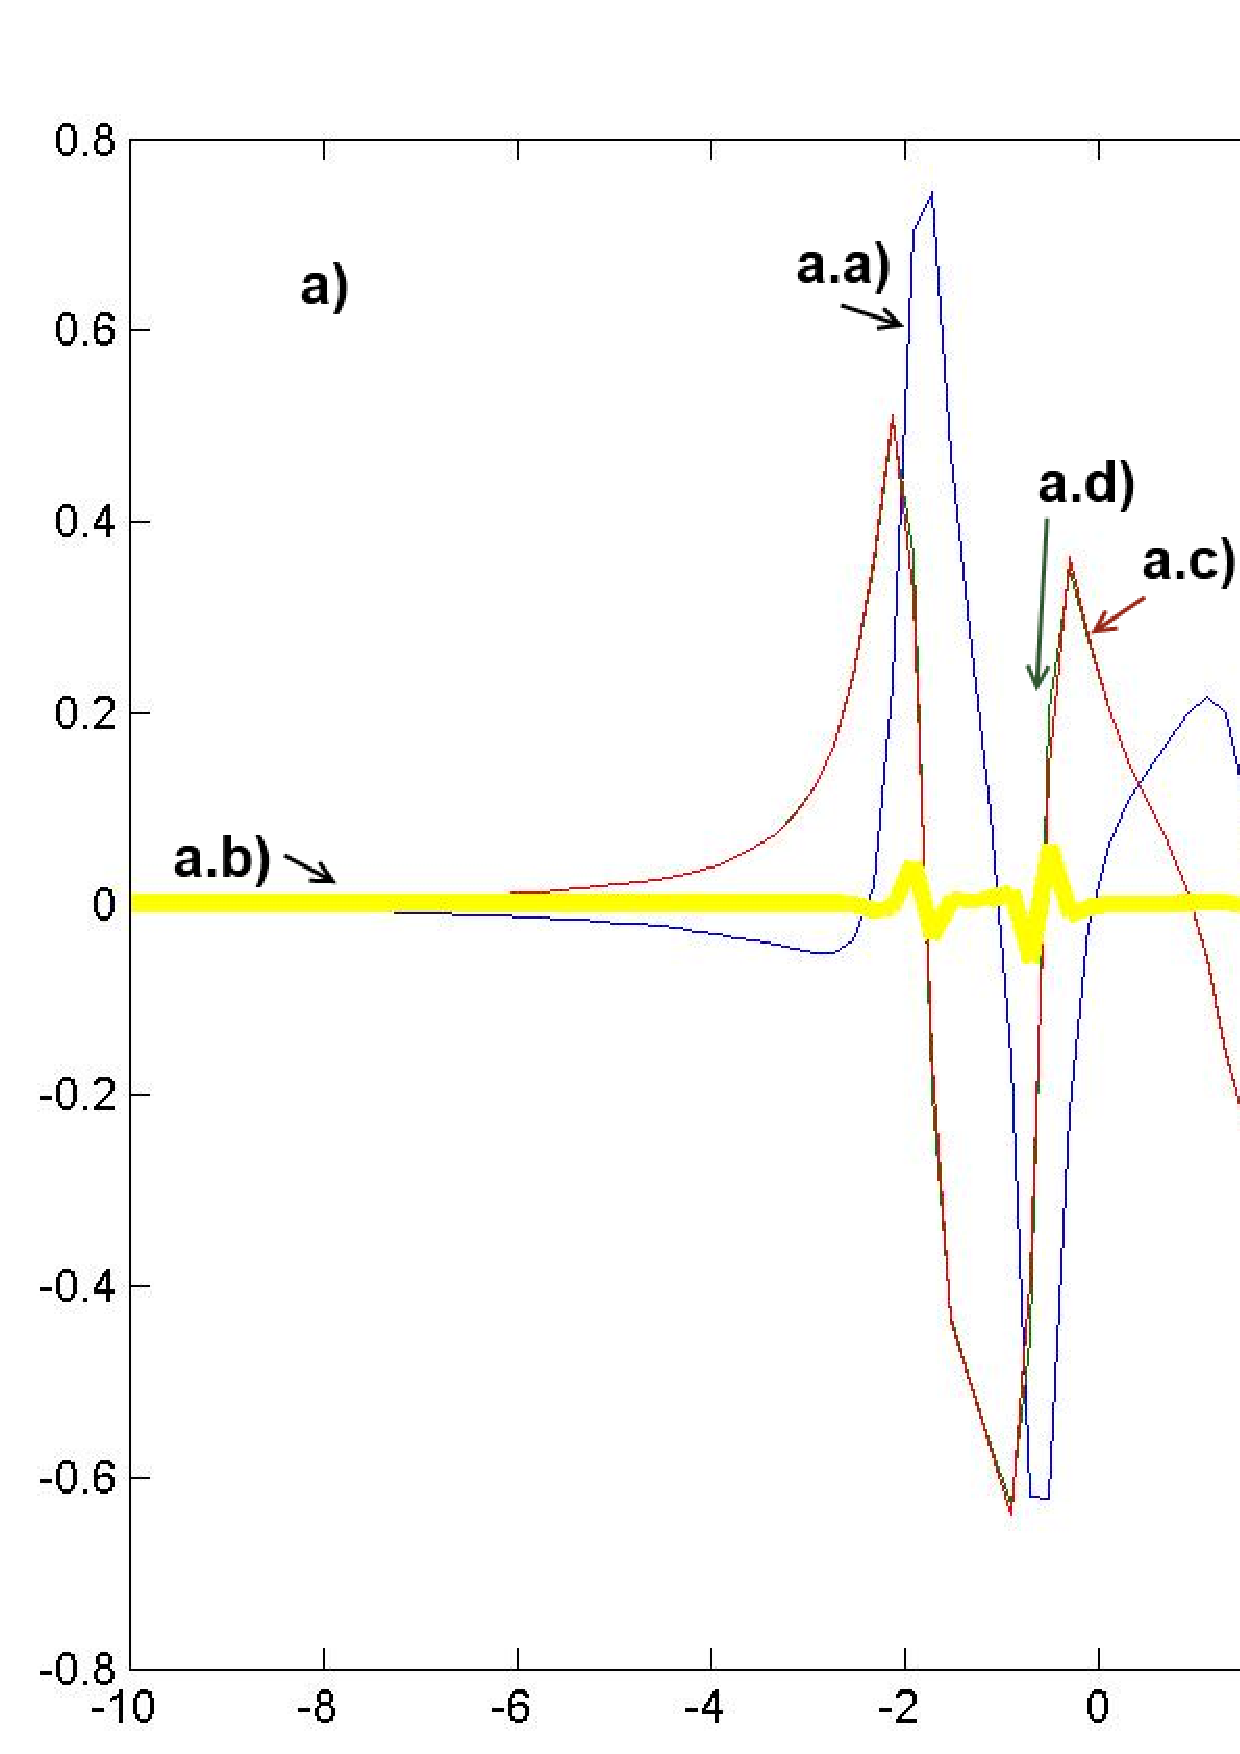
\includegraphics[width=150mm]{img/hcc_fmix.png}
  \caption{Results for the frequency mixing model using the Hilbert Clenshaw-Curtis iterations
     a.a) The plot of the real part of ${\chi_{mix}}(\delta )$
     a.b) absolute error plot (a.d-plot minus a.c-plot) 
     a.c) imaginary part of ${\chi_{mix}}(\delta )$ calculated analytically 
     a.d) imaginary part of ${\chi_{mix}}(\delta )$ obtained with the Hilbert transform of a.a-plot, 
     b.a) The plot of the imaginary part of ${\chi_{mix}}(\delta )$ 
     b.b) absolute error plot (b.d-plot minus b.c-plot) 
     b.c) real part of $\chi_{mix} (\omega )$ calculated analytically 
     b.d) real part of ${\chi_{mix}}(\delta )$ obtained with the Hilbert transform of b.a-plot 
     \label{fig:hcci_fmix}
     }
\end{figure}

As we can see here - once again the results come with quite well accuracy.

\subsection{HCCI for simple quantum-perturbative model} \label{chap:hcc_quantum}
 
\subsubsection*{Linear model - results:}

As in the Chapter (\ref{chap:nc_nlo}), we have used the same model to describe the simple linear quantum-perturbative model: 

\begin{equation} \label{eq:hcc_qp}
  {\chi_{1, \,qp}}(\omega ) = \frac {N}{\varepsilon_0\,h} \sum_{n=1}^{2}\,(\frac {{\mu_{1, \,n}}\,{ \mu_{2, \,n}}}{{\Omega_{n}}
  - \omega  - i\,{\gamma_{n}}} + \frac {{\mu_{2, \,n}}\,{\mu_{1, \,n}}}{{\Omega_{n}} + \omega + i\,{\gamma_{n}}})
\end{equation}

This time we used the following parameters: \\
$\mu = [[3, \, - 0.5], \,[1.2, \,2.4]]$, 
$\Omega = [ - 3, \,13]$, \, 
$\gamma = [0.7, \,2.3]$, \,
$N = 8$, \,
$\varepsilon_{0} = 1.4,$, \, 
$h = - 2.7$ .

Results are presented in Figure (\ref{fig:hcc_qp1}). We can see a perfect match here!

\begin{figure}
  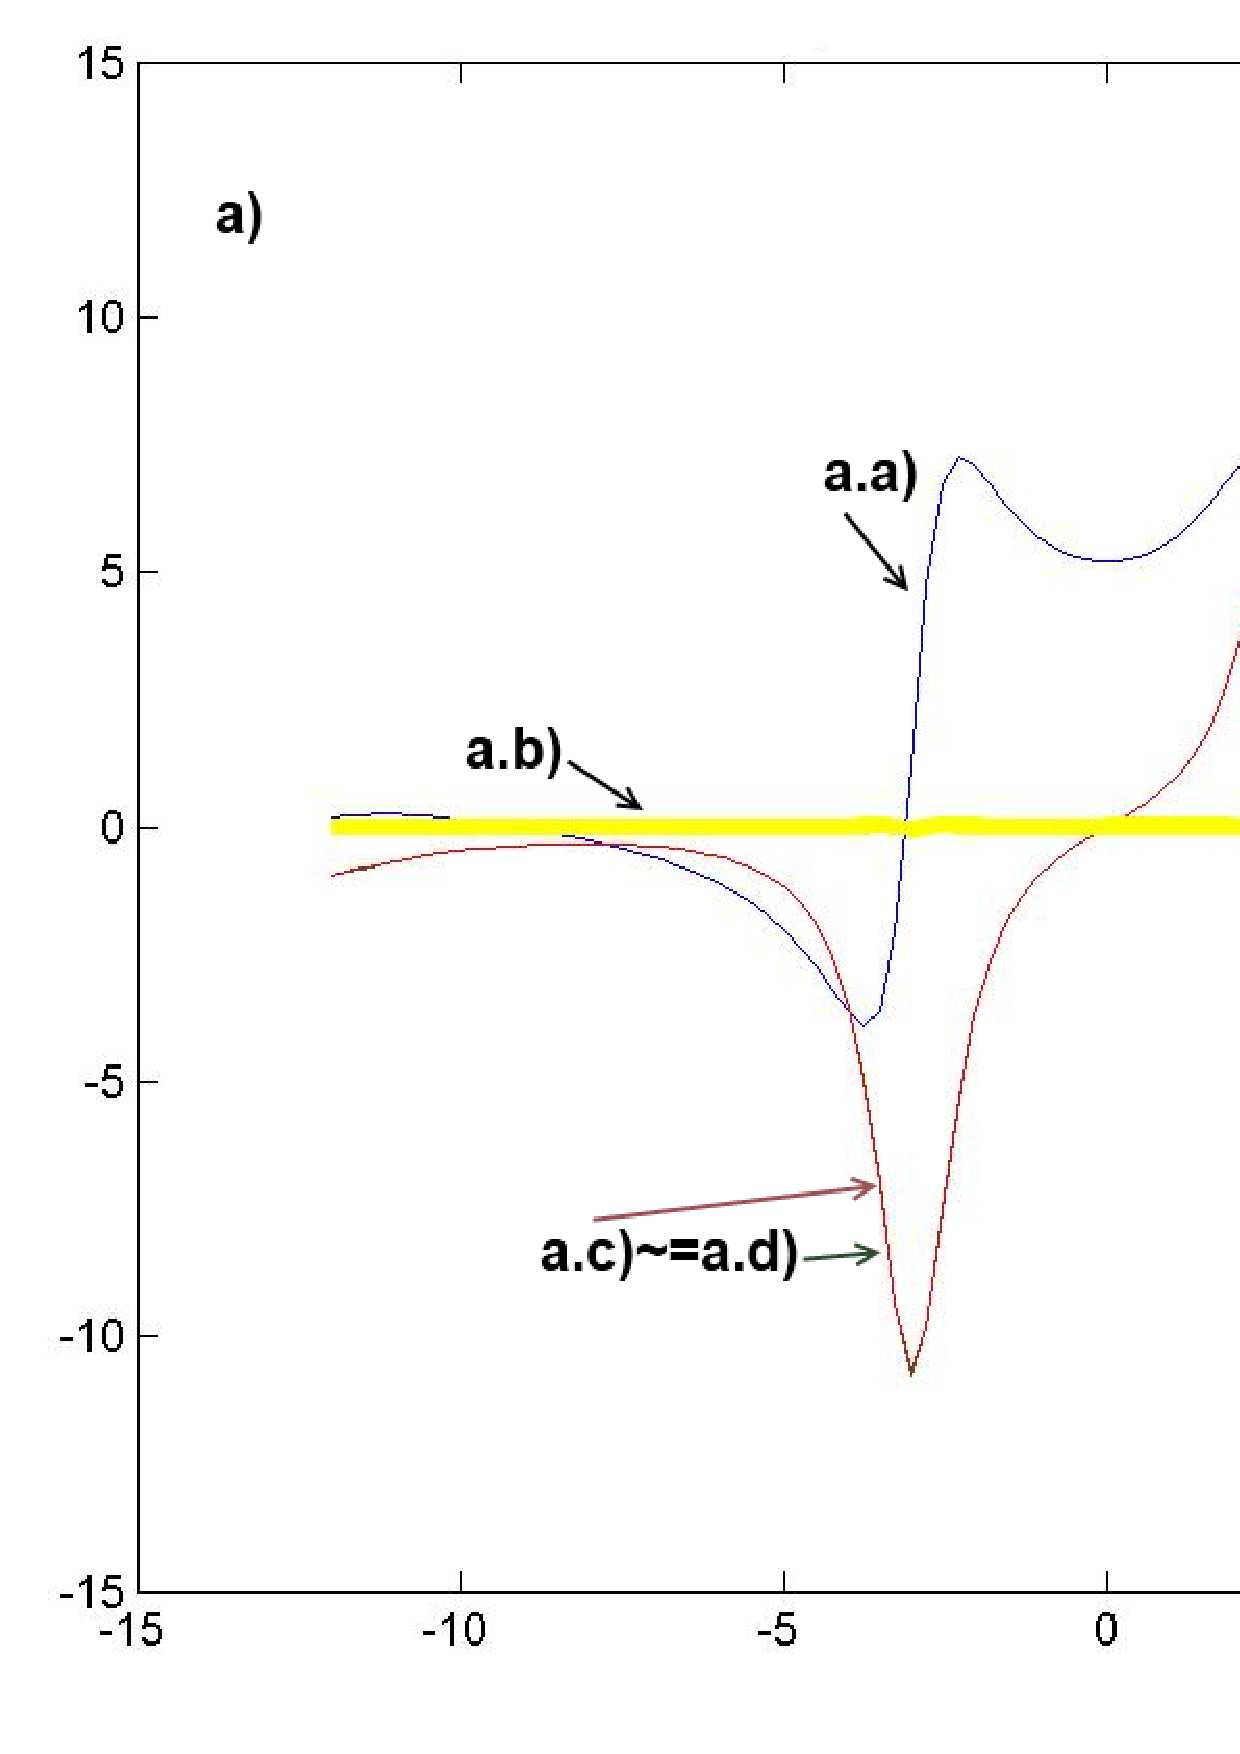
\includegraphics[width=150mm]{img/hcc_qp1.png}
  \caption{Results for the linear quantum perturbative model for HCCI quadrature
    a.a) The plot of the imaginary part of ${\chi_{1, \, qp}}(\omega )$
    a.b) absolute error plot (d-plot minus c-plot) 
    a.c) real part of ${\chi_{1, \, qp}}(\omega )$ obtained with the Hilbert transform of a-plot 
    a.d) real part of ${\chi_{1, \, qp}}(\omega )$ calculated analytically 
    b.b) The plot of the real part of ${\chi_{1, \, qp}}(\omega )$ 
    b.b) absolute error plot (d-plot minus c-plot) 
    b.c) imaginary part of ${\chi_{1, \, qp}}(\omega )$ obtained with the Hilbert transform of a-plot 
    b.d) imaginary part of ${\chi_{1, \, qp}}(\omega )$ calculated analytically  
    \label{fig:hcc_qp1}
  }
\end{figure}

\subsubsection*{Second-order model - results:}

We have also used the same model as in Chapter (\ref{chap:nc_nlo}) to describe the second-order susceptibility model:

\begin{multline} \label{hcc_qp2}
  \chi_{2, \,qp}({\omega_{1}}, \,{\omega_{2}}) = 
  2\,N\,\varepsilon_{0}\,h^{2}\,\sum_{n=1}^{2}\sum_{m=1}^{2}\sum_{l=1}^{2}\,
  (
       \frac {{\mu_{l,\,n}}\,{\mu_{nm}}\,{\mu_{ml}}}
      {({\Omega_{nl}} - \omega_1 - \omega_2 - i\,{\gamma_{nl}})\,({\Omega_{ml}} - \omega_1 - i\,{\gamma_{ml}})} +
+ \\ + \frac {{\mu_{l, \,n}}\,{\mu_{nm}}\,{\mu_{ml}}}
      {({\Omega_{nl}} - \omega_1 - \omega_1 - i\,{\gamma_{nl}})\,({\Omega_{ml}} - \omega_2 - i\,{\gamma_{ml}})}
+ \\ + \frac {{\mu_{l, \,n}}\,{\mu_{nm}}\,{\mu_{ml}}}
      {({\Omega_{mn}} - \omega_1 - \omega_2 - i\,{\gamma_{mn}})\,({\Omega_{nl}} + \omega_2 + i\,{\gamma_{nl}})}
+ \\ + \frac {{\mu_{l, \,n }}\,{\mu_{nm}}\,{\mu_{ml}}} 
      {({\Omega_{mn}} - \omega_1 - \omega_2 - i\,{\gamma_{mn}})\,({\Omega_{nl}} + \omega_2 + i\,{\gamma_{nl}})} 
+ \\ + \frac {{\mu_{l, \,n}}\,{\mu_{nm}}\,{\mu_{ml}}}
      {({\Omega_{nm}} + \omega_1 + \omega_2 + i\,{\gamma_{nm}})\,({\Omega_{ml}} - \omega_1 - i\,{\gamma_{ml}})}
+\\ + \frac {{\mu_{l, \,n}}\,{\mu_{ nm}}\,{\mu_{ml}}}
      {({\Omega_{nm}} + \omega_1 + \omega_2 + i\,{\gamma_{nm}})\,({\Omega_{ml}} - \omega_1 - i\,{\gamma_{ml}})} 
+ \\ + \frac {{\mu_{l, \,n}}\,{\mu_{nm}}\,{\mu_{ml}}}
      {({\Omega_{ml}} + \omega_1 + \omega_2 + i\,{\gamma_{ml}})\,({\Omega_{nl}} + \omega_1 + i\,{\gamma_{nl}})}
+\\ + \frac {{\mu_{l, \,n}}\,{\mu_{nm}}\,{\mu_{ml}}}
      {({\Omega_{ml}} + \omega_1 + \omega_2 + i\,{\gamma_{ml}})\,({\Omega_{nl}} + \omega_2 + i\,{\gamma_{nl}})}
  )  
\end{multline}

for the defined set of parameters:

\begin{equation}
	\mu = \left| \begin{array}{cc} 
    1 & 3 \\ -1 & -2 
  \end{array} \right|, \, 
  \Omega = \left| \begin{array}{cc} 
    3 & 16 \\ 4 & 12 
  \end{array} \right|, \,
  \gamma = \left| \begin{array}{cc} 
  1 & 2 \\ -1 & 3
  \end{array} \right|, \,
  N = 5, \, 
  \varepsilon_0 = 1, \,
  h= - 1
\end{equation}

Results are presented in Figure (\ref{fig:hcc_qp2}). As for the Newton-Cotes calculations in Chapter (\ref{chap:nc_quantum}) we can
see the model could be invalid because the arisen errors reach up to 100\%. 

\begin{figure} 
  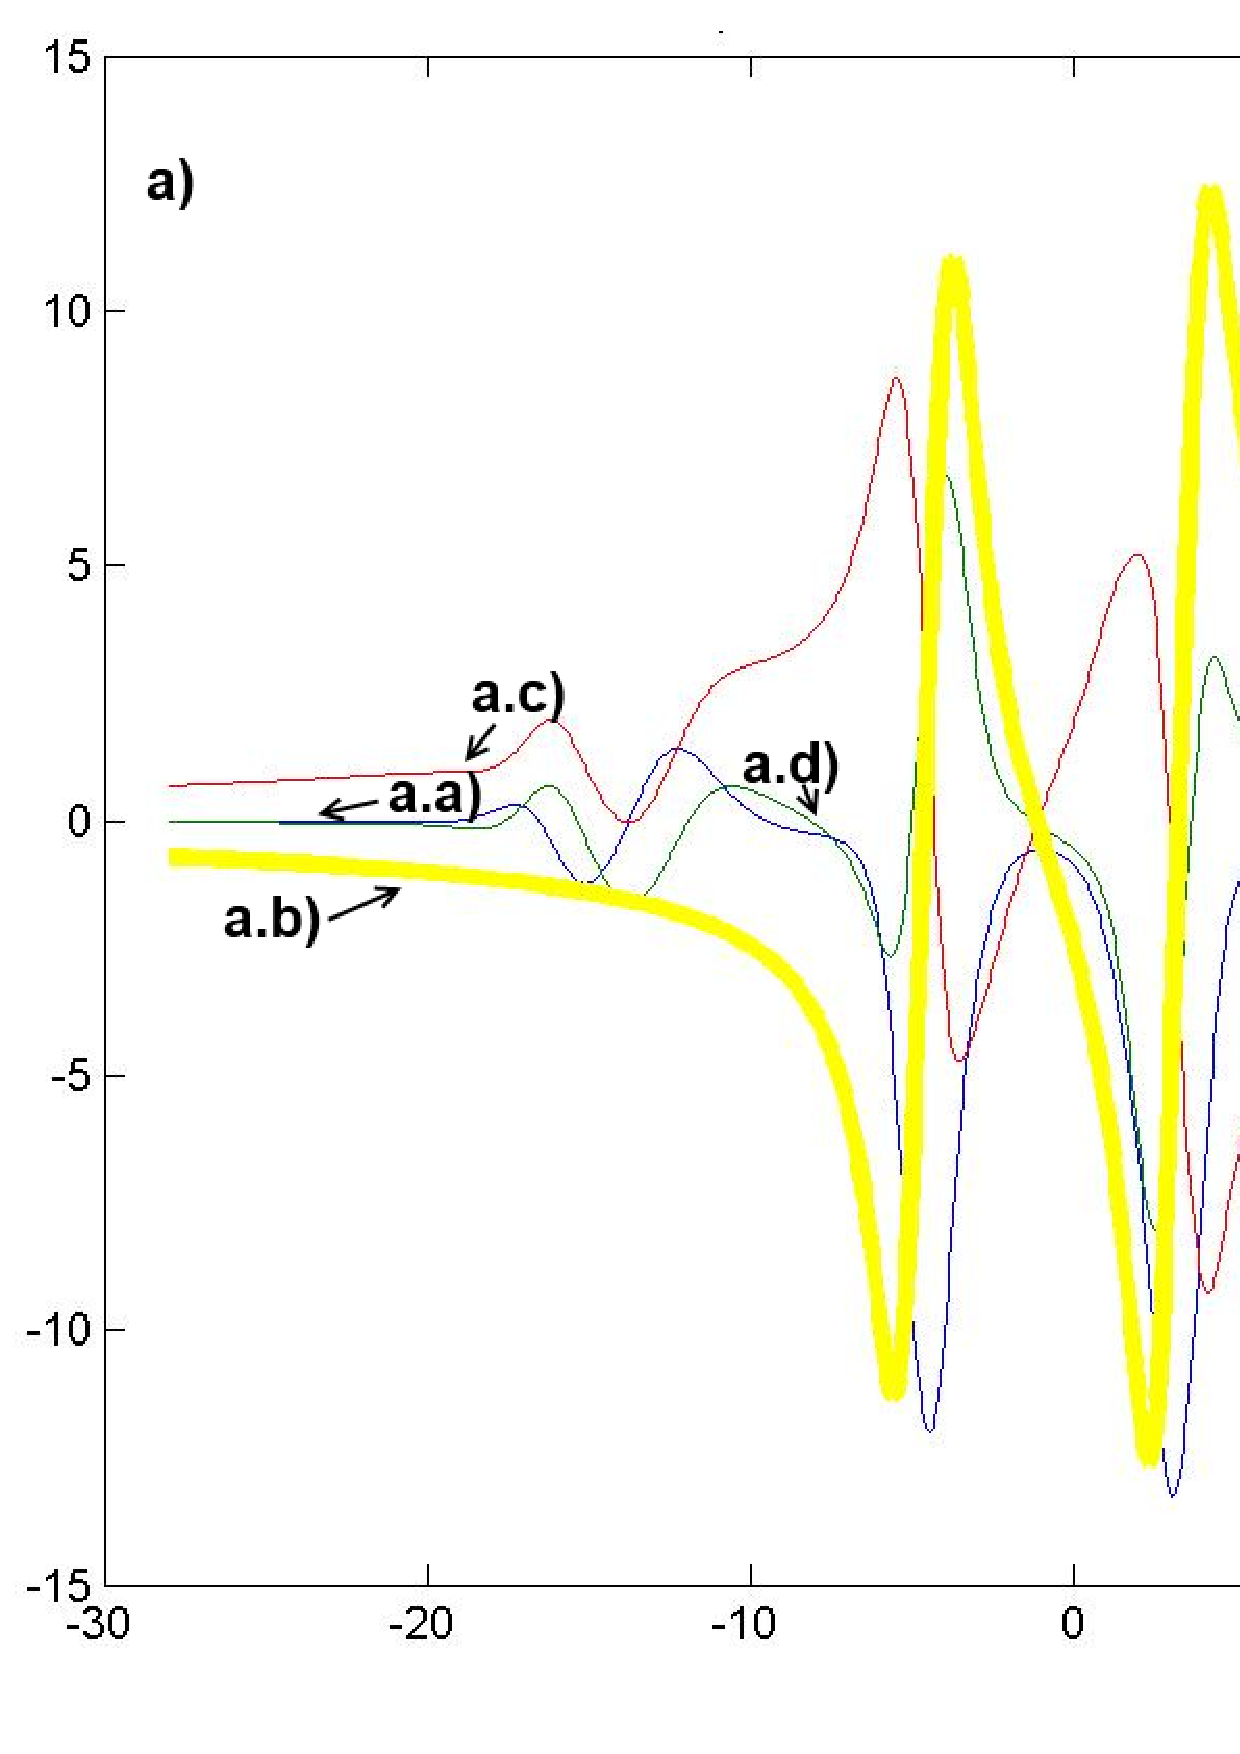
\includegraphics[width=150mm]{img/hcc_qp2.png}
  \caption{Results for the second-order quantum perturbative model for HCCI quadrature
     a.a) The plot of the real part of $\chi_{2, \, qp} (\omega )$
     a.b) absolute error plot (a.d-plot minus a.c-plot) 
     a.c) imaginary part of $\chi_{2, \, qp} (\omega )$ calculated analytically 
     a.d) imaginary part of $\chi_{2, \, qp} (\omega )$ obtained with the Hilbert transform of a.a-plot, 
     b.a) The plot of the imaginary part of ${\chi_{2, \,qp}}(\omega )$ 
     b.b) absolute error plot (b.d-plot minus b.c-plot) 
     b.c) real part of $\chi_{2, \, qp} (\omega )$ calculated analytically 
     b.d) real part of $\chi_{2, \, qp} (\omega )$ obtained with the Hilbert transform of b.a-plot 
     \label{fig:hcc_qp2}
     }
\end{figure}


\section{Fast Hartley transform approach} \label{chap:hartley}

\subsection{Overview of the FTHA} \label{chap:hartley_overview}

The Fast Hartley Transform approach for the Hilbert transform is based on two efficient O (n log n) discrete Hartley transforms and
was well described by Soo-Chang Pei in \cite{chang_computation}. This approach is faster than another discrete Hilbert transform
based on two Fourier transforms, because the whole computation are carried using only real numbers, which is faster than Fourier
computation carried using time consuming complex numbers.

\subsubsection*{Discrete Hartley Transform}

For a given N-length vector X both the discrete Hartley transform and inverse discrete Hartley transform are defined as follows:

\begin{subequations} \label{eq:fhta_definition}
  \begin{equation}   \label{eq:fhtadef_dht}
    \mathrm{DHT}(X_k) = \sum_{n = 0}^{N - 1} \, X_n \, (
      \mathrm{cos} \left(\frac {2 \, \pi \, k \, n}{N} \right) 
    + \mathrm{sin} \left(\frac {2 \, \pi \, k \, n}{N} \right) )
  \end{equation}
  \begin{equation}   \label{eq:fhtadef_idht}
    \mathrm{IDHT}({H_{k}})= \frac {1}{N} \sum_{k = 0}^{N - 1} \, H_n \, (
    	\mathrm{cos} \left( \frac {2 \, \pi \, k \, n}{N} \right) 
      + \mathrm{sin} \left( \frac {2 \, \pi \, k \, n}{N} \right) ) 
  \end{equation}
\end{subequations}

\subsubsection*{Hartley transform convolution theorem}

Now we will introduce the Hartley transform convolution theorem. We define the N-length vector x as convolution of two N-length
vectors ${x_{1}}$, ${x_{2}}$ as follows:

\begin{equation} \label{eq:hartley_convolution}
  x_n = x_{1, \,n} \convolution x_{2, \,n} = \sum_{k = 0}^{N - 1} \, x_{1, \, k} \, x_{2, \, n - k} 
\end{equation}

For a given convolution, the following theorem is stated:

\begin{equation} \label{eq:hartley_theorem}
  \mathrm{DHT}(x_n) = \mathrm{DHT}(x_{1, \,  k}) \, \mathrm{even}(\mathrm{DHT}(x_{2, \, k})) 
                    + \mathrm{DHT}(x_{1, \, -k}) \, \mathrm{odd} (\mathrm{DHT}(h_{2, \, k})),
\end{equation}

with: $\mathrm{DHT}(x_{2, \,k}) = \mathrm{even}(\mathrm{DHT}(x_{2, \,k})) 
                                 + \mathrm{odd} (\mathrm{DHT}(x_{2, \,k}))$

The proof of the Hartley transform convolution theorem can be found in \cite{chang_computation}. 

\subsubsection*{Relation between discrete Fourier and discrete Hilbert transform}

To better understand the relation between the discrete Fourier and discrete Hilbert transform we will introduce the dicrete Hilbert kernel:

\begin{equation}   \label{eq:hdfttps_smallh}
	h_k = \frac {1}{\pi \, k} \, \mbox{ discrete Hilbert kernel } .  
\end{equation}

The discrete Fourier transform of the discrete Hilbert kernel will be marked with the symbol $\mathrm{H}(k)$ :

\begin{equation}   \label{eq:hdfttps_bigh}
    \mathrm{H}(k) = \mathrm{DFT}(h_k), 
\end{equation}

and the $\mathrm{H}$ has the following properties:

\begin{subequations} \label{eq:hartley_defh}
  \begin{equation}   \label{eq:hdefh_fhalf}
    \mathrm{H}(k) =  i \, \mbox{ for } \, k = 1, \, 2, \, \ldots, \, \frac {N}{2} - 1 ,
  \end{equation}
  \begin{equation}   \label{eq:hdefh_middle}
    \mathrm{H}(k) =  0 \, \mbox{ for } \, k = 0, \, \frac {N}{2} ,
  \end{equation}
  \begin{equation}   \label{eq:hdefh_shalf}
    \mathrm{H}(k) = -i \, \mbox{ for } \, k = \frac {N}{2} + 1, \, \frac {N}{2} + 2, \, \ldots, \, N - 1
  \end{equation} .
\end{subequations}

We derive the discrete Fourier transform of the Hilbert transform for a given N-length vector x:

\begin{equation} \label{eq:hartley_dfttheorem}
  \mathrm{DFT}(\mathrm{DISCRETE\_HILBERT}(x_k)) = 
  	\mathrm{H}(k) \, \mathrm{DFT}(x_k)  = ( - i) \, \mathrm{\text{sgn}}(k) \, \mathrm{DFT}(x_k) .
\end{equation}

\subsubsection*{Application of the discrete Hartley transform to calculate the discrete Hilbert transform:}

Using the Hartley transform convolution theorem (\ref{eq:hartley_defh}) for a given N-length vector x we obtain:

\begin{multline} \label{eq:hartley_fullconvolution}
         \mathrm{DHT}(\mathrm{DISCRETE\_HILBERT}(x_k))  
  = \\ = \mathrm{DHT}(x_{k})   \, \mathrm{even}(\mathrm{DHT}(h_k)) 
       + \mathrm{DHT}(x_{- k}) \, \mathrm{odd} (\mathrm{DHT}(h_k)),
\end{multline} 

where we have use the time reversal notation: $ x_{ - k} = x_{(N - k) \, \mathrm{mod} \, N}$.

Now we should notice, that the discrete Hilbert transform kernel defined in (\ref{eq:hdfttps_smallh}) is an odd function, so its even
part equals zero. So (\ref{eq:hartley_fullconvolution}) simplifies now into a product of two separate Hartley transforms:

\begin{equation} \label{eq:hartley_simpleconvolution}
  \mathrm{DHT}(\mathrm{DISCRETE\_HILBERT}(x_k))=\mathrm{DHT}(x_{ - k})\,\mathrm{odd}(\mathrm{DHT}(h_k)) =
  \mathrm{DHT}(x_{- k})\,\mathrm{DHT}(h_k)
\end{equation}

By \cite{chang_computation} the second transform is defined:

\begin{subequations} \label{eq:hartley_strans} 
  \begin{equation}   \label{eq:hstrans_fhalf}
    \mathrm{DHT}(h_k) =  1 \, \mbox{ for } \, k = 1, \, 2, \, \ldots, \, \frac {N}{2} - 1
  \end{equation}
  \begin{equation}   \label{eq:hstrans_middle}
    \mathrm{DHT}(h_k) =  0 \, \mbox{ for } \, k = 0, \, \frac {N}{2}
  \end{equation}
  \begin{equation}   \label{eq:hstrans_shalf}
    \mathrm{DHT}(h_k) = -1 \, \mbox{ for } \, k = \frac {N}{2} + 1, \, \frac {N}{2} + 2 .. N - 1
  \end{equation}
\end{subequations}

In order to calculate the Hilbert of a given N-length vector x the last thing to do is to apply the inverse discrete Hartley
transform on the very right side of (\ref{eq:hartley_simpleconvolution}) equation.

\subsubsection*{Fast Hartley Transform algorithm}

Ronald F. Ullmann has showed the fast algorithm for the discrete Hartley transform in~\cite{ullmann_algorithm}. The important
assumption is that - as for the fast Fourier transform algorithm, the fast Hartley transform algorithm is defined for a K-length
vector x, where K is the power-of-two:

\begin{equation} \label{eq:ullmand_existp}
  \exists p\,\ \in\ \,N : K=2^{p}
\end{equation}


The (\ref{eq:ullmand_existp}) condition for the algorithm and the further possibilities to modify it are discussed further. We will
start with the very same thing as in the fast Fourier algorithm - we split the x vector into two smaller vectors:

\begin{subequations} \label{eq:hartley_smallervectors}
  \begin{equation}   \label{eq:hsvs_even}
    x_{1, \, \frac     {m}{2}} = x_m \, \mbox{ for } \, m = 0, \, 2, \, \ldots, \, N - 1
  \end{equation}
  \begin{equation}   \label{eq:hsvs_odd}
    x_{2, \, \frac {m - 1}{2}} = x_m \, \mbox{ for } \, m = 1, \, 3, \, \ldots, \, N - 2
  \end{equation}
\end{subequations}

Taking into account the initial definition of the discrete Hartley transform (\ref{eq:fhtadef_dht}), we obtain:

\begin{multline}  \label{eq:hartley_longdht}
 \mathrm{DHT}(x_k) = \left( 
 	\sum_{n = 0}^{\frac {N}{2} - 1} \, \mathrm{x}(2 \, n) \, (
 		\mathrm{cos} \left( \frac {2 \, \pi \, k \, 2 \, n}{N} \right) 
  	  + \mathrm{sin} \left( \frac {2 \, \pi \, k \, 2 \, n}{N} \right) ) \right)  
 + \\ \left( 
 	\sum_{n = 0}^{\frac {N}{2} - 1} \, \mathrm{x}(2 \, n + 1) \, (
 		\mathrm{cos} \left( \frac {2 \, \pi \, k \, (2 \, n + 1)}{N} \right) 
 	  + \mathrm{sin} \left( \frac {2 \, \pi \, k \, (2 \, n + 1)}{N} \right) ) \right)
\end{multline}

In \cite{ullmann_algorithm} the following ''shift rule'' for the discrete Hartley transform is stated :

\begin{equation} \label{eq:hartley_shiftrule}
  \mathrm{DHT}(x_{k + c}) = \mathrm{DHT}(x_k) \, \mathrm{cos}(c)
 + \mathrm{DHT}(x_{ - k}) \, \mathrm{sin}(c)
\end{equation}

If we apply the Hartley shift rule (\ref{eq:hartley_shiftrule}) to the split equation in (\ref{eq:hartley_longdht}) we obtain:

\begin{multline} \label{eq:hartley_srapplied}
  \mathrm{DHT}(x_k) = \mathrm{DHT}(x_{1, \, k}) 
  	+ \mathrm{cos} \left( \frac {2 \, \pi \, k}{N} \right) \, \mathrm{DHT}(x_{2, \,k}) +
      \mathrm{sin} \left( \frac {2 \, \pi \, k}{N} \right) \, \mathrm{DHT}(x_{2, \, - k})\, \\
  \mbox{ for } \, k=0, \, 1, \, 3, \, \ldots, \frac {N}{2} - 1
\end{multline}

The rule (\ref{eq:hartley_srapplied}) can be applied only for the half of the possible k values ($k < \frac{N}{2}$). Now we will use
the periodic properties of the discrete Hartley transform kernel:

\begin{subequations} \label{eq:hartley_kernel}
  \begin{equation}   \label{eq:hkern_plus}
    \mathrm{cos} \left(   \frac {2 \, \pi \, k \,      (n + N)}{N} \right) + 
    \mathrm{sin} \left(   \frac {2 \, \pi \, k \, 2 \, (n + N)}{N} \right) =
    \mathrm{cos} \left(   \frac {2 \, \pi \, k \, n}{N} \right) + 
    \mathrm{sin} \left(   \frac {2 \, \pi \, k \, 2 \, n}{N} \right)
  \end{equation}
  \begin{equation}   \label{eq:hkern_minus}
    \mathrm{cos} \left(   \frac {2 \, \pi \, k \,      (n + \frac {N}{2})}{N} \right)  + 
    \mathrm{sin} \left(   \frac {2 \, \pi \, k \, 2 \, (n + \frac {N}{2})}{N} \right) = 
    - \left( \mathrm{cos}(\frac {2 \, \pi \, k \, n}{N}) +
             \mathrm{sin}(\frac {2 \, \pi \, k \, 2 \, n}{N}) 
      \right)
  \end{equation}
\end{subequations}


The rule (\ref{eq:hartley_srapplied}) using the periodicity property from (\ref{eq:hartley_kernel}) can be now used for all k indices:

\begin{subequations} \label{eq:hartley_periodicity}
  \begin{equation}   \label{eq:hperiod_fhalf}
    \mathrm{DHT}(x_k) = \mathrm{DHT}(x_{1, \,k}) 
    	+ \mathrm{cos} \left( \frac {2 \, \pi \, k}{N} \right) \, \mathrm{DHT}(x_{2, \, k}) +
          \mathrm{sin} \left( \frac {2 \, \pi \, k}{N} \right) \, \mathrm{DHT}(x_{2, \, - k})
  \end{equation}
  
  for $ \, k = 0, \,1,\dotsc,\frac {N}{2} - 1$
  \begin{multline}   \label{eq:hperiod_shalf}
    \mathrm{DHT}(x_k) = \\
        \mathrm{DHT}(x_{1, \,k - \frac {N}{2}}) 
      - \mathrm{cos} \left( \frac {2\,\pi \,(k - \frac{N}{2})}{N} \right) \, \mathrm{DHT}(x_{2, \,   k - \frac {N}{2}}) 
      - \mathrm{sin} \left( \frac {2\,\pi \,(k - \frac{N}{2})}{N} \right) \, \mathrm{DHT}(x_{2, \, - k + \frac {N}{2}})
  \end{multline}
  
  for \,$k = \frac {N}{2}, \, \frac {N}{2} + 2, \dotsc, \, N - 1$
\end{subequations}
 
The remaining definition for the negative index, need to be explained:

\begin{equation} \label{eq:hartley_negindex}
  \mathrm{DHT}(v_{ - k}) = \mathrm{DHT}(v_{(N - k) \, \mathrm{mod} \, N})
\end{equation}

Of course this is a typical divide-and-conquer approach, where the complexity is reduced from $\mathrm{O}(n^{2}) \, $ to
$ \, \mathrm{O}(n \, \mathrm{log}(n))$, very similar to the approach used in the Cooley-Tukey FFT algorithm \cite{Tukey_algorithm}.

\subsubsection*{Non-power-of-two case}

There are several approaches when calculating the fast Fourier transform for a non-power-of-two case length of the input x vector. 
One approach PFA is the Good-Thomas \cite{Good_interaction} / prime-factor algorithm for a vector length K defined:

\begin{equation}  \label{eq:hartley_goodk}
  K = K_1 \, K_2 ,
\end{equation}

Where $K_1$ and $K_2$ are relatively prime numbers. Another approach was presented by Leo Bluestein, called also the chirp
z-transform algorithm is presented in \cite{bluestein_linear}. Another author, George Bruun, has invented the approach based on
the recursive polynomial-factorization in \cite{bruun_ztransform}. Rader has prepared the special FFT algorithm especially for
vectors of prime size in \cite{rader_dicrete}. But we will use the simplest possible approach - called the zero-padding. So in case
of input vector with the size of non-power-of-two, we add the suffix vector filled with vectors to fit the next possible
power-of-two size. In the worst case, the input vector size will be doubled, which has no influence on the asymptotic complexity,
which remains O(n log n). While the discrete signal analysis is the domain of scientists, we will end with conclusion stated by M.
Lamb in \cite{lamb_issues} that he is uncertain, if zero padding has an influence on the spectral resolution, but in most cases it
has a little influence on the results obtained in the discrete transforms.

The source code of the discrete Hilbert transform using both the fast Hartley transform and inverse fast Hartley transform has been
presented in Appendix A.4.

\subsection{FTHA for simple linear model} \label{chap:hartley_lin}

In Figure (\ref{fig:fht_lin}) we have presented the results obtained with the Fast Hartley Hilbert Transform for the simple
linear model defined in model (\ref{eq:physical_frequency_linear}). As we can see - the Fast Hartley Hilbert Transform gives us quite well
accuracy, similar to HCCI and much better than HTRAN or Newton-Cotes quadrature. 

\begin{figure} 
  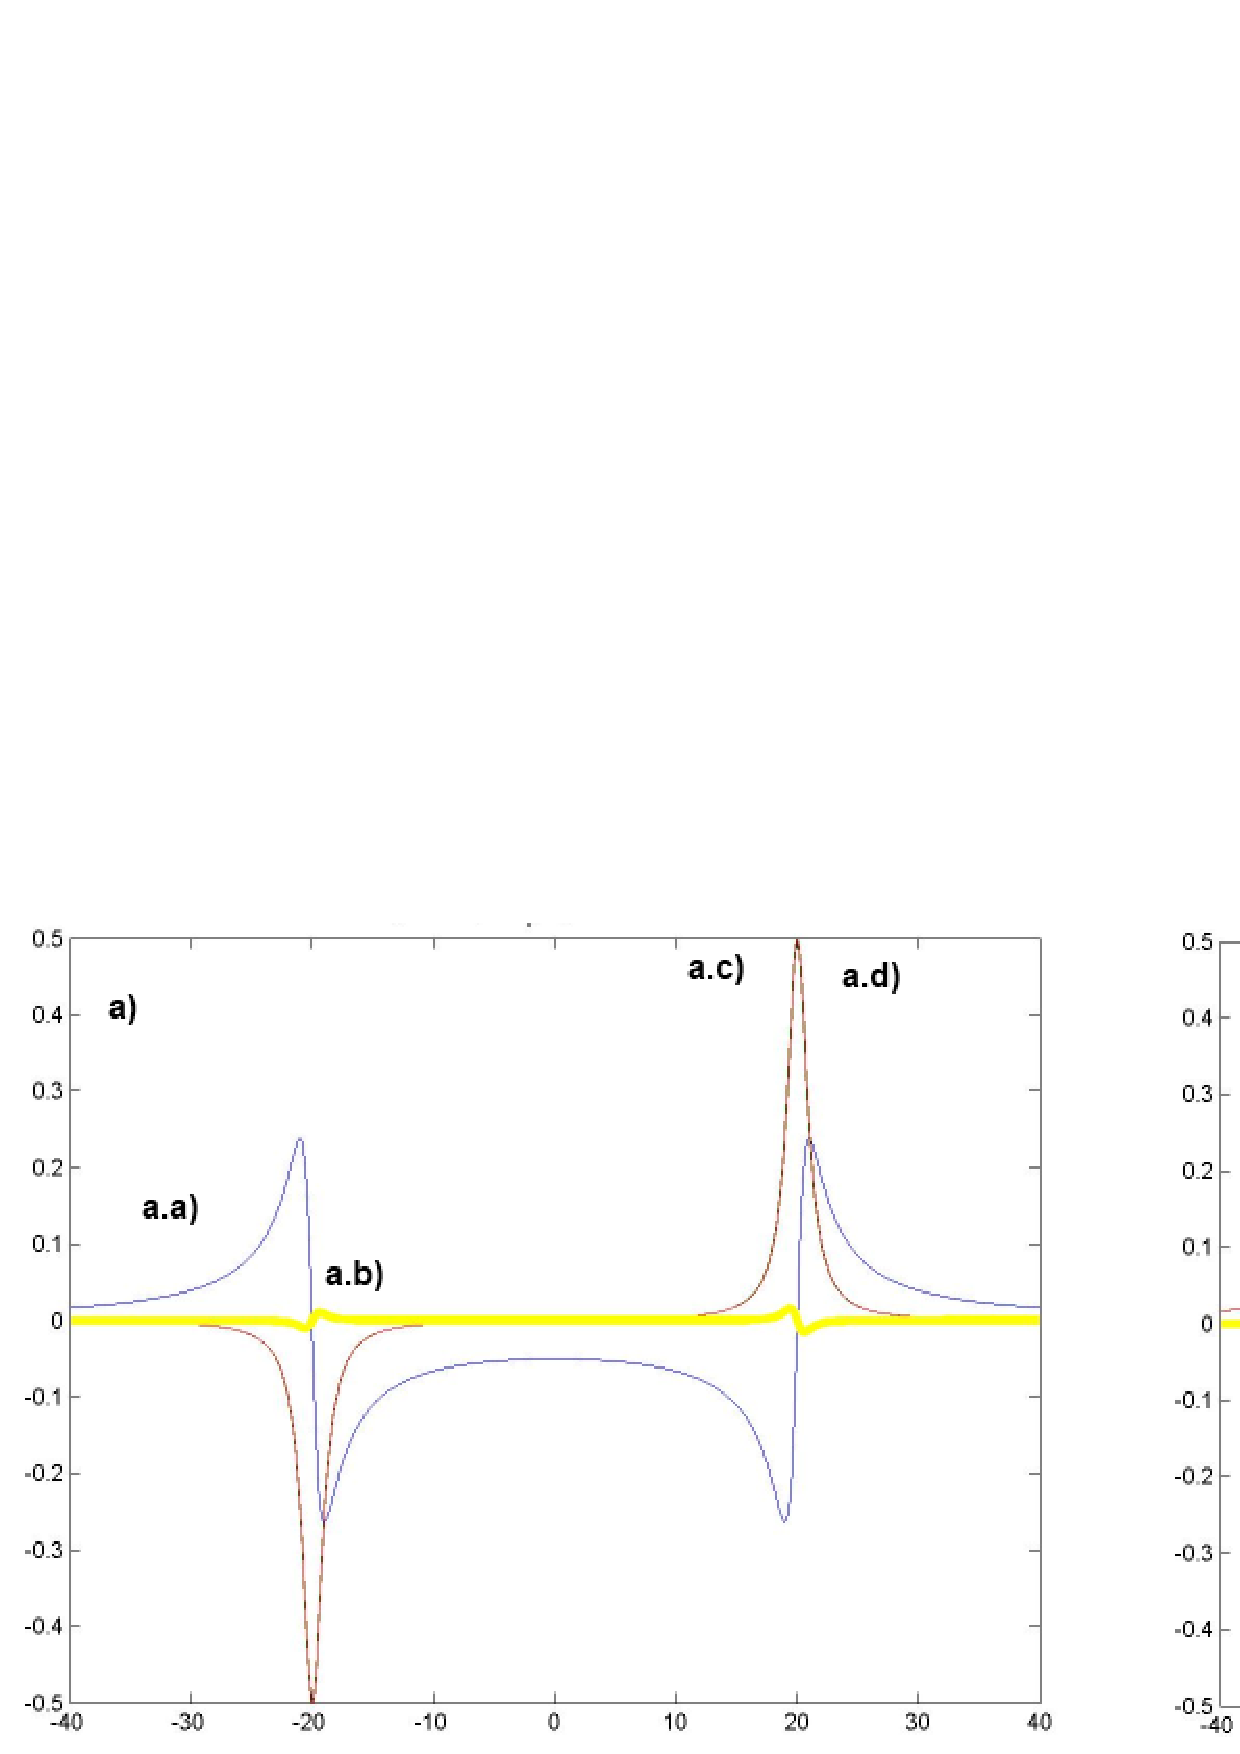
\includegraphics[width=150mm]{img/fht_lin.png}
  \caption{The Figure presents the results of the Fast Hartley Hilbert Transform method applied to the simple linear
  model. Results are plotted together.
   a.a) The plot of the real part of $\chi (\omega )$ 
   a.b) absolute error plot (c-plot minus d-plot) 
   a.c) imaginary part of $\chi (\omega )$ obtained with the Hilbert transform of a-plot 
   a.d) imaginary part of $\chi (\omega )$  calculated analytically. 
   b.a) The plot of the imaginary part of $\chi (\omega )$ 
   b.b) absolute error plot (c-plot minus d-plot) 
   b.c) real part of $\chi (\omega )$ obtained with the Hilbert transform of a-plot 
   b.d) real part of $\chi (\omega )$ calculated analytically. \label{fig:fht_lin}
  }
\end{figure}

\subsection{FTHA for simple nonlinear model} \label{chap:hartley_nlo}

For the pump-probe and frequency mixing models we have used the same parameters as in Chapter (\ref{chap:nc_nlo}). The results
obtained with the Fast Hartley Hilbert Transform has been presented in Figures (\ref{fig:fht_pnp}) and (\ref{fig:fht_fmix})
respectively.

\begin{figure} 
  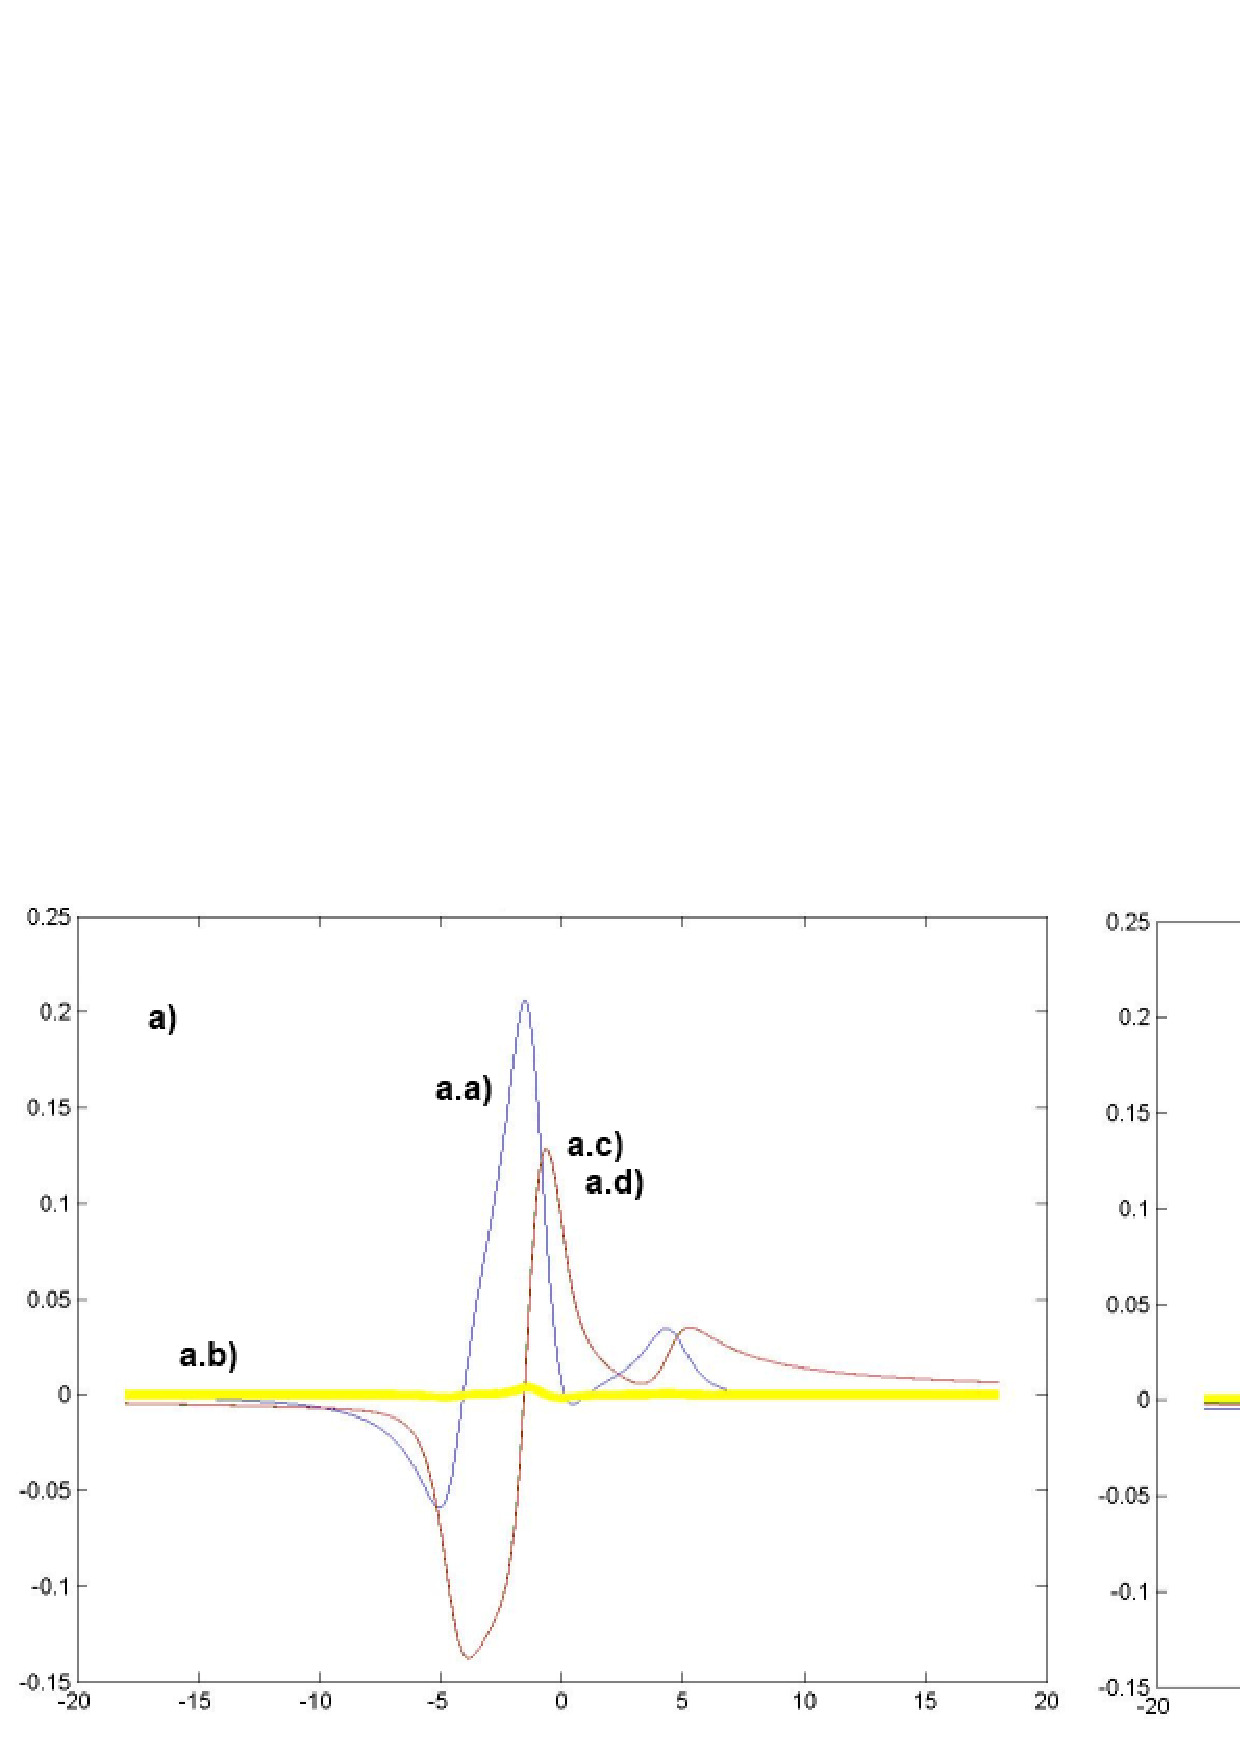
\includegraphics[width=150mm]{img/fht_pnp.png}
  \caption{The Figure presents the results of the Fast Hartley Hilbert Transform method applied to the pump-and-probe model. Results are
  plotted together.
     a.a) The plot of the real part of ${\chi_{pp}}(\omega )$
     a.b) absolute error plot (a.d-plot minus a.c-plot) 
     a.c) imaginary part of $\chi_{pp}(\omega )$ calculated analytically 
     a.d) imaginary part of $\chi_{pp}(\omega )$ obtained with the Hilbert transform of a.a-plot, 
     b.a) The plot of the imaginary part of $\chi_{pp}(\omega )$ 
     b.b) absolute error plot (b.d-plot minus b.c-plot) 
     b.c) real part of $\chi_{pp} (\omega )$ calculated analytically 
     b.d) real part of $\chi_{pp} (\omega )$ obtained with the Hilbert transform of b.a-plot 
     \label{fig:fht_pnp}
     }
\end{figure} 

\begin{figure} 
  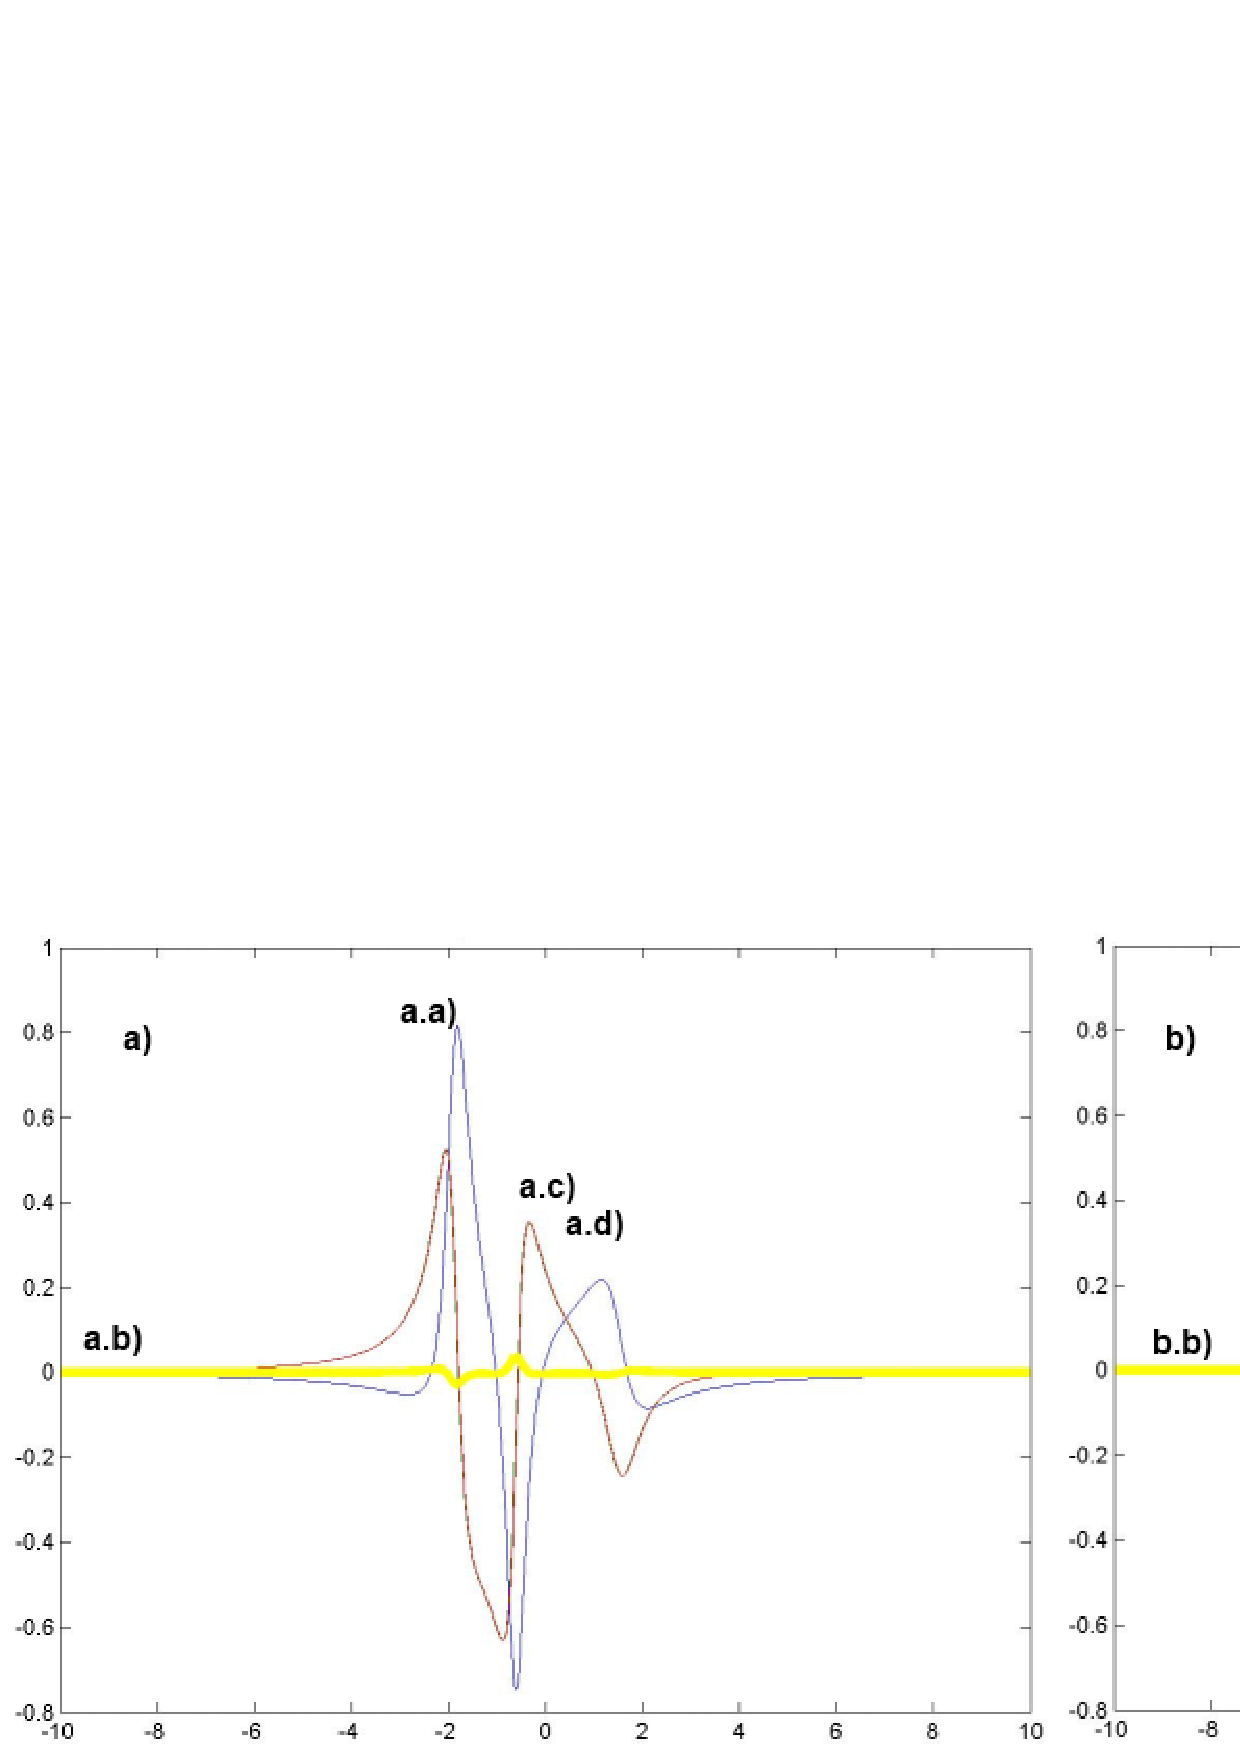
\includegraphics[width=150mm]{img/fht_fmix.png}
  \caption{The Figure presents the results of the Fast Hartley Hilbert Transform method applied to the frequency mixing model. Results are
  plotted together.
     a.a) The plot of the real part of ${\chi_{mix}}(\delta )$
     a.b) absolute error plot (a.d-plot minus a.c-plot) 
     a.c) imaginary part of $\chi_{mix}(\omega )$ calculated analytically 
     a.d) imaginary part of $\chi_{mix}(\omega )$ obtained with the Hilbert transform of a.a-plot, 
     b.a) The plot of the imaginary part of $\chi_{mix}(\omega )$ 
     b.b) absolute error plot (b.d-plot minus b.c-plot) 
     b.c) real part of $\chi_{mix} (\omega )$ calculated analytically 
     b.d) real part of $\chi_{mix} (\omega )$ obtained with the Hilbert transform of b.a-plot 
     \label{fig:fht_fmix}
     }
\end{figure}

Once again we can see a very good accuracy, better than for HTRAN or Newton-Cotes, and similar to HCCI.

\subsection{FTHA for simple quantum-perturbative model} \label{chap:hartley_quantum}

\subsubsection*{Linear model - results:}

As in the Chapter (\ref{chap:nc_nlo}), we have used the same model to describe the simple linear quantum-perturbative model: 

\begin{equation} \label{eq:fht_qp}
  {\chi_{1, \,qp}}(\omega ) = \frac {N}{\varepsilon_0\,h} \sum_{n=1}^{2}\,(\frac {{\mu_{1, \,n}}\,{ \mu_{2, \,n}}}{{\Omega_{n}}
  - \omega  - i\,{\gamma_{n}}} + \frac {{\mu_{2, \,n}}\,{\mu_{1, \,n}}}{{\Omega_{n}} + \omega + i\,{\gamma_{n}}})
\end{equation}

This time we used the following parameters: \\
$\mu = [[3, \, - 0.5], \,[1.2, \,2.4]]$, 
$\Omega =[ - 3, \,13]$, 
$\gamma =[0.7, \,2.3]$,  
$N=8$, 
${\varepsilon_{0}}=1.4, 
h= - 2.7$

Results are presented in Figure (\ref{fig:fht_qp1}). We can see a perfect match here!

\begin{figure}
  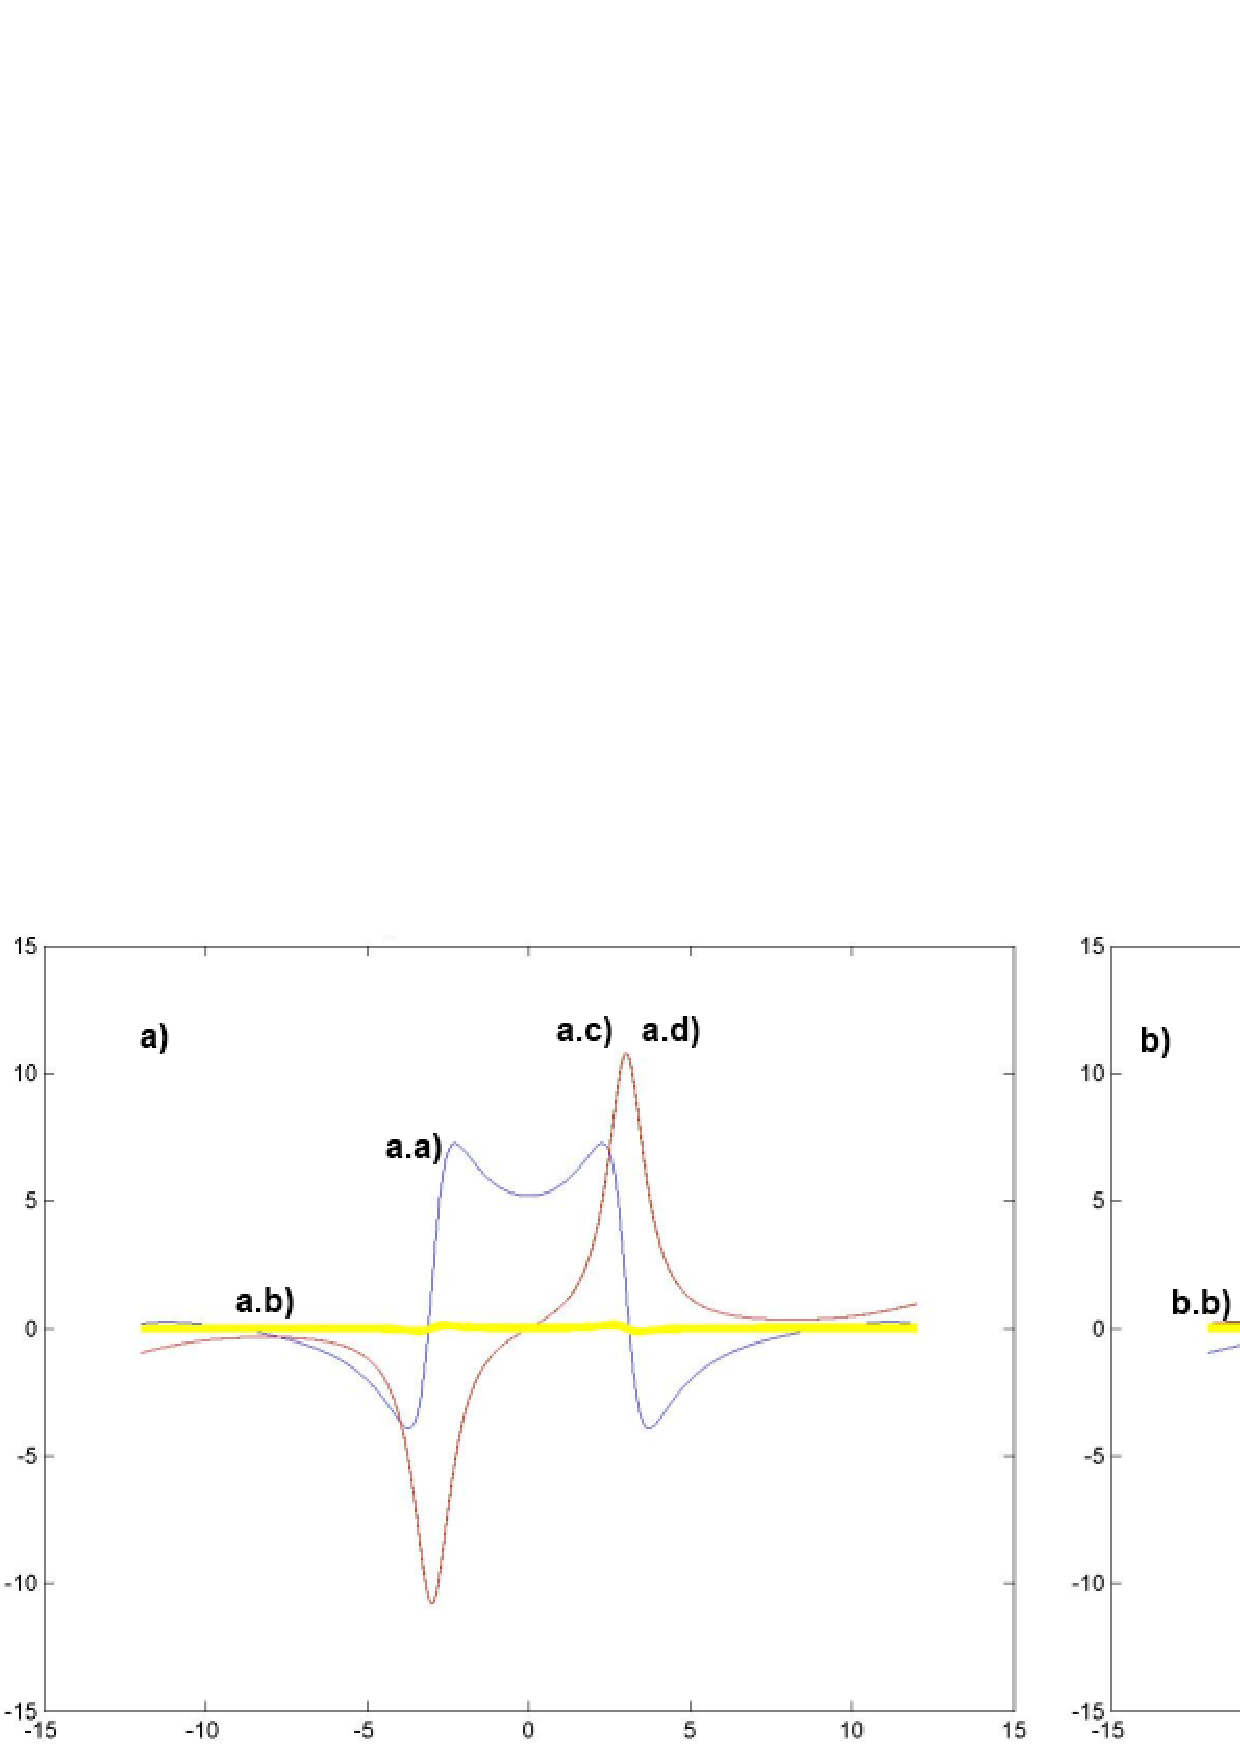
\includegraphics[width=150mm]{img/fht_qp1.png}
  \caption{Results for the linear quantum perturbative model for FHT Hilbert transform
    a.a) The plot of the imaginary part of ${\chi_{1, \,qp}}(\omega )$
    a.b) absolute error plot (d-plot minus c-plot) 
    a.c) real part of $\chi_{1, \, qp} (\omega )$ obtained with the Hilbert transform of a-plot 
    a.d) real part of $\chi_{1, \, qp} (\omega )$ calculated analytically 
    b.b) The plot of the real part of $ \chi_{1, \, qp} (\omega )$ 
    b.b) absolute error plot (d-plot minus c-plot) 
    b.c) imaginary part of $\chi_{1, \, qp} (\omega )$ obtained with the Hilbert transform of a-plot 
    b.d) imaginary part of $\chi_{1, \, qp} (\omega )$ calculated analytically  
    \label{fig:fht_qp1}
  }
\end{figure}

\subsubsection*{Second-order model - results:}

We have also used the same model as in Chapter (\ref{chap:nc_nlo}) to describe the second-order susceptibility model:

\begin{multline} \label{eq:fht_qp2}
  \chi_{2, \,qp}({\omega_{1}}, \,{\omega_{2}}) = 
     2\,N\,\varepsilon_{0}\,h^{2}\,\sum_{n=1}^{2}\sum_{m=1}^{2}\sum_{l=1}^{2}\,
  ( 
      \frac {{\mu_{l,\,n}}\,{\mu_{nm}}\,{\mu_{ml}}}
      {({\Omega_{nl}} - \omega_1 - \omega_2 - i\,{\gamma_{nl}})\,({\Omega_{ml}} - \omega_1 - i\,{\gamma_{ml}})}
+\\ + \frac   {{\mu_{l, \,n}}\,{\mu_{nm}}\,{\mu_{ml}}}
      {({\Omega_{nl}} - \omega_1 - \omega_1 - i\,{\gamma_{nl}})\,({\Omega_{ml}} - \omega_2 - i\,{\gamma_{ml}})}
+\\ + \frac   {{\mu_{l, \,n}}\,{\mu_{nm}}\,{\mu_{ml}}}
      {({\Omega_{mn}} - \omega_1 - \omega_2 - i\,{\gamma_{mn}})\,({\Omega_{nl}} + \omega_2 + i\,{\gamma_{nl}})}
+\\ + \frac{{\mu_{l, \,n }}\,{\mu_{nm}}\,{\mu_{ml}}} 
      {({\Omega_{mn}} - \omega_1 - \omega_2 - i\,{\gamma_{mn}})\,({\Omega_{nl}} + \omega_2 + i\,{\gamma_{nl}})} 
+\\ + \frac   {{\mu_{l, \,n}}\,{\mu_{nm}}\,{\mu_{ml}}}
      {({\Omega_{nm}} + \omega_1 + \omega_2 + i\,{\gamma_{nm}})\,({\Omega_{ml}} - \omega_1 - i\,{\gamma_{ml}})}
+\\ + \frac {{\mu_{l, \,n}}\,{\mu_{ nm}}\,{\mu_{ml}}}
      {({\Omega_{nm}} + \omega_1 + \omega_2 + i\,{\gamma_{nm}})\,({\Omega_{ml}} - \omega_1 - i\,{\gamma_{ml}})} 
+\\ + \frac {{\mu_{l, \,n}}\,{\mu_{nm}}\,{\mu_{ml}}}
      {({\Omega_{ml}} + \omega_1 + \omega_2 + i\,{\gamma_{ml}})\,({\Omega_{nl}} + \omega_1 + i\,{\gamma_{nl}})}
+\\ + \frac {{\mu_{l, \,n}}\,{\mu_{nm}}\,{\mu_{ml}}}
      {({\Omega_{ml}} + \omega_1 + \omega_2 + i\,{\gamma_{ml}})\,({\Omega_{nl}} + \omega_2 + i\,{\gamma_{nl}})}
  )  ,
\end{multline}
and we have used the following values of the constants: \\
$\mu = \left| \begin{array}{cc} 
    1 & 3 \\ -1 & -2 
  \end{array} \right|,\, 
  \Omega = \left| \begin{array}{cc} 
    3 & 16 \\ 4 & 12 
  \end{array} \right|,\,
  \gamma = \left| \begin{array}{cc} 
  1 & 2 \\ -1 & 3
  \end{array} \right|,\, N=5,\, {\varepsilon_{0}}=1,\,h= - 1$

Results are presented in Figure (\ref{fig:fht_qp2}). As for the previous calculations, we can see the model could be invalid
because of the raised errors reach up to 100\%.

\begin{figure} 
  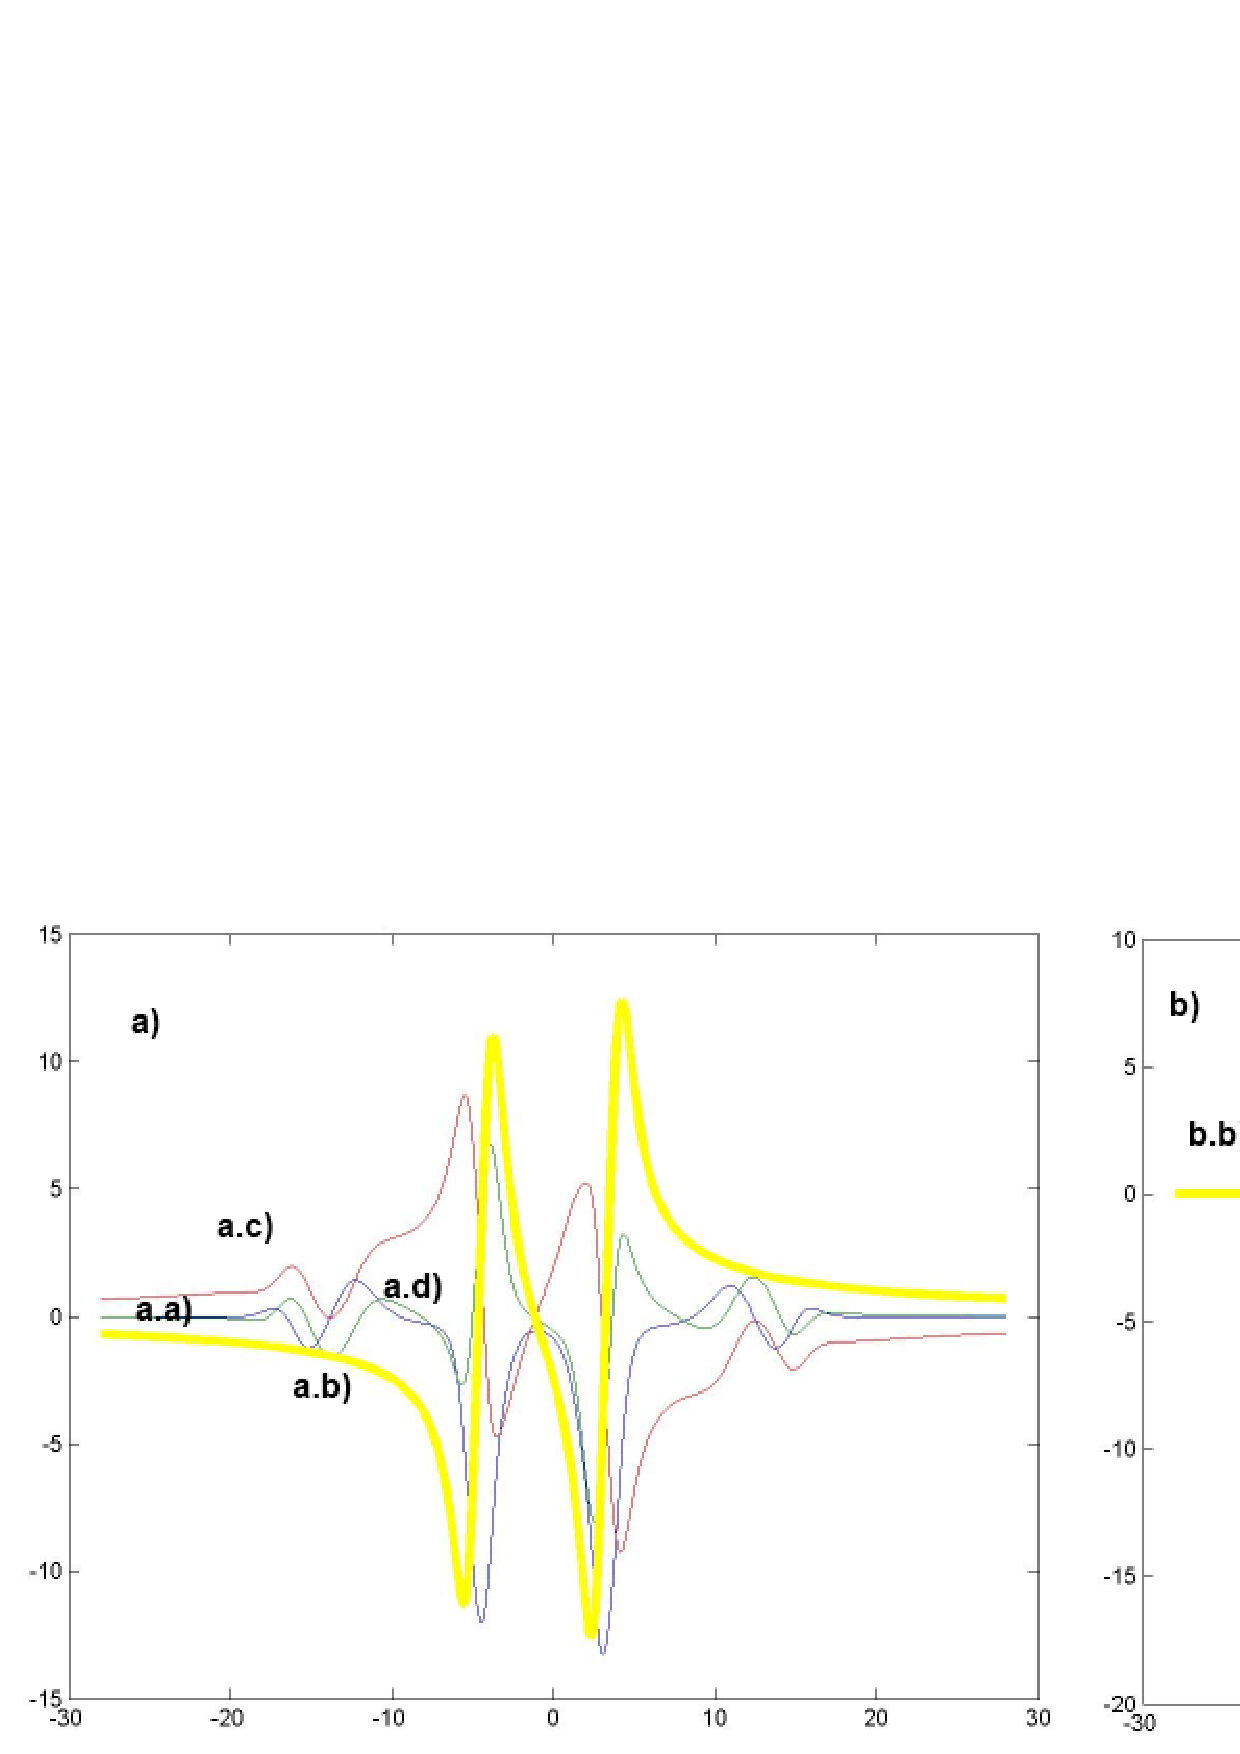
\includegraphics[width=150mm]{img/fht_qp2.png}
  \caption{Results for the second-order quantum perturbative model for FHT Hilbert transform
     a.a) The plot of the real part of $\chi_{2, \, qp}(\omega )$
     a.b) absolute error plot (a.d-plot minus a.c-plot) 
     a.c) imaginary part of $\chi_{2, \, qp}(\omega )$ calculated analytically 
     a.d) imaginary part of $\chi_{2, \, qp}(\omega )$ obtained with the Hilbert transform of a.a-plot, 
     b.a) The plot of the imaginary part of $\chi_{2, \, qp}(\omega )$ 
     b.b) absolute error plot (b.d-plot minus b.c-plot) 
     b.c) real part of $\chi_{2, \, qp} (\omega )$ calculated analytically 
     b.d) real part of $\chi_{2, \, qp} (\omega )$ obtained with the Hilbert transform of b.a-plot 
     \label{fig:fht_qp2}
     }
\end{figure}

\section{Hermite-Hilbert transform} \label{chap:hermite}

\subsection{Overview of the HHT}  \label{chap:hermite_overview}

Hermite-Hilbert transform approach is based on the precalculation of already-known Hermite polynomials and Hermite base of orthogonal
functions. The algorithm is based on the master thesis of Mathias Johansson \cite{johansson_hilbert}.

\subsubsection*{Hermite polynomials and Hermite functions:}

Hermite polynomial of an arbitrary n degree is defined as follows:

\begin{equation} \label{eq:hermite_definition}
	H_n(x) = \frac {( - 1)^{n} \, e ^ {(x ^ 2)} \, d ^ n \, e^{( - x ^ 2)} } {{dt}^{n}}
\end{equation}

There is also an recursive equation for Hermite polynomials:

\begin{subequations} \label{eq:hermite_recursive}
  \begin{equation}   \label{eq:hrec_next}
    H_n (x) = 2 \, x \, H_{n - 1}(x) + 2 \, (n - 1) \, H_{n - 2}(x)
  \end{equation}
  \begin{equation}   \label{eq:hrec_first}
    H_0 (x) = 1
  \end{equation}
\end{subequations}

Using the Hermite polynomial we would like to derive a set of orthogonal polynomials in $L ^ 2$. Therefore we introduce the
weight function and the norm function:

\begin{subequations} \label{eq:hermite_weight}
  \begin{equation}   \label{eq:hwht_weight}
    \mathrm{w}(x) = e^{( - \frac {x^{2}}{2})}
  \end{equation}
  \begin{equation}   \label{eq:hwht_iter}
    N_n (x) = \sqrt{2^{n} \, n\mathrm{!} \, \sqrt{\pi }}
  \end{equation}
\end{subequations}

If we multiply the n-th Hermite polynomial with the weight function w(x) and divide it by the n-th norm function $N_n$ we
obtain a n-th orthogonal Hermite function:

\begin{equation} \label{eq:hermite_orthogonal}
  \phi_n (x) = \frac {\mathrm{w}(x) \, H_n (x)} {N_n (x)} 
  	= \frac {e^{( - \frac {x ^ 2}{2})} \, H_n (x)} {\sqrt{2^{n} \, n\mathrm{!} \, \sqrt {\pi }}}
\end{equation}

Based on the recursive equation in (\ref{eq:hermite_recursive}) we also obtain:

\begin{subequations} \label{eq:hermite_recresult}
  \begin{equation}   \label{eq:hrr_weight}
    \phi_n (x) = \sqrt{\frac {2 \, x \, {\phi_{n - 1}}(x)}{n}} - (n - 1) \, \sqrt{\frac {{\phi_{n - 2}}(x)} {(n - 1) \, n}}
  \end{equation}
  \begin{equation}   \label{eq:hrr_iter}
    \phi_0 (x) = \frac {e^{( - \frac {x ^ 2} {2})}} {\pi ^{(\frac {1}{4})}}
  \end{equation}
\end{subequations}

\subsubsection*{Hilbert transform of Hermite functions:}

Johansson after polish mathematician Stefan L. Hahn \cite{hahn_hilbert} states that for any f(x) and
$\mathrm{HILBERT}(\mathrm{f}(x))$ belonging to $ L_1 $ we have:

\begin{equation} \label{eg:hermite_hproperty}
  \mathrm{HILBERT}(x \, \mathrm{f}(x)) = x \, \mathrm{HILBERT}(\mathrm{F}(x)) 
    - \frac {1}{\pi } \, \int_{ - \infty } ^ {\infty}\mathrm{f}(\tau ) \, d\tau 
\end{equation}

The proof of the Theorem stated in (\ref{eg:hermite_hproperty}) is short:

\begin{equation} \label{eq:hermite_hpropproof}
  \mathrm{HILBERT}(x \, \mathrm{f}(x)) = 
  	\frac{1}{\pi } \, \dashint_{ - \infty }^{ \infty } \frac {\tau \,    \mathrm{f}(\tau )} {x - \tau} \, d\tau  
  = \frac{1}{\pi } \, \dashint_{ - \infty }^{ \infty } \frac {(x - s) \, \mathrm{f}(x - s)} {s} \, ds ,
\end{equation}
\begin{alignat*}{1}
  \mbox { where } \, s &= x - \tau = 
  	\frac{1}{\pi } \, \dashint_{ - \infty }^{ \infty } \frac {x \, \mathrm{f}(x - s)}{s} \, ds -
    \frac{1}{\pi } \, \dashint_{ - \infty }^{ \infty } \mathrm{f}(x - s) \, ds = \\
  &= x \, \mathrm{HILBERT}(\mathrm{f}(x)) 
  - \frac{1}{\pi } \, \dashint_{ - \infty }^{ \infty } \mathrm{f}(\tau ) \, d\tau 
\end{alignat*}

From both equations (\ref{eg:hermite_hproperty}) and (\ref{eq:hermite_recresult}) we now obtain the important result:

\begin{subequations} \label{eq:hermite_impresult}
  \begin{equation}   \label{eq:hir_phinext}
    \mathrm{HILBERT}( \phi_n (x)) = \sqrt{\frac {2} {n}} \, 
    	\left( x \, \phi_{n - 1} (x) - \frac {1}{\pi } \, \int_{ - \infty }^{ \infty } {\phi_{n - 1}}(\eta )\,d\eta  \right)  
    	- (n - 1) \, \sqrt{\frac {1}{n \, (n - 1)}} \, \phi_{n - 2} (x)
  \end{equation}
  \begin{equation}   \label{eq:hir_phifirst}
    \mathrm{HILBERT}(\phi_{0} (x)) = 2 \, \sqrt{2} \, \pi ^{(\frac {1}{4} )} \, 
    	\int_{0}^{\infty } e ^ {( - \frac {\omega ^ 2} {2})} \, \mathrm{sin} (\omega \, x) \, d\omega
  \end{equation}
\end{subequations}

\subsubsection*{Hilbert transform based on the Hermite functions:}

Now we can derive the Hilbert transform of an arbitrary function. We start with expanding f = f(x) into a series sum:

\begin{subequations} \label{eq:hermite_fexpand}
  \begin{equation}   \label{eq:hfe_f}
     \mathrm{f}(x) = \sum_{n = 0}^{\infty } \, a_n \, \phi_n(x) 
  \end{equation}
  \begin{equation}   \label{eq:hfe_an}
     a_n(x) = \int_{ - \infty }^{\infty } \mathrm{f}(x) \, \phi_n (x) \, dx
  \end{equation}
\end{subequations}

For each function that has a limited series expansion at infinity we can provide an estimation used in further numerical algorithm:

\begin{subequations} \label{eq:hermite_estimate}
  \begin{equation}   \label{eq:hest_fapprox}
      f(x) \approx \sum_{n = 0}^{N} \, a_n \, \phi_n (x)
  \end{equation}
  \begin{equation}   \label{eq:hest_happrox}
     \mathrm{HILBERT} (\mathrm{f}(x)) \approx \sum_{n = 0} ^ {N} \, a_n \, \mathrm{HILBERT}(\phi_n (x))
  \end{equation}
\end{subequations}

\subsubsection*{Short description of the numerical algorithm:}

Taking a look on the (\ref{eq:hermite_estimate}) we can see that the only difficulty is to calculate the $a_n$ coefficients,
while both the $\phi_n (x)$ and $\mathrm{HILBERT}(\phi_n (x))$ can be precalculated once. The integral in
(\ref{eq:hermite_fexpand}) is now much easier because there is no singularity. The algorithm is given in Appendix A.5 and it
consists of three main parts:

\begin{tabular}{l l}
  1.         & PRECALCULATION of the Hermite function \\
             & coefficients with Maple Toolbox \\
  MAIN LOOP: & \\
  2.         & ESTIMATION OF ${a_{n}}$ COEFFICIENTS \\
  3.         & CALCULATION OF THE HILBERT TRANSFORM (\ref{eq:hest_happrox}) \\
\end{tabular}

\subsection{HHT for simple linear model} \label{chap:hermite_lin}

In Figure (\ref{fig:hht_lin}) we have presented the results obtained with the Hermite-Hilbert transform for the simple
linear model defined in model (\ref{eq:physical_frequency_linear}). As we can see - the Hermite-Hilbert transform comes with poor accuracy,
but we would like to put this method into examination with defined models.

\begin{figure} 
  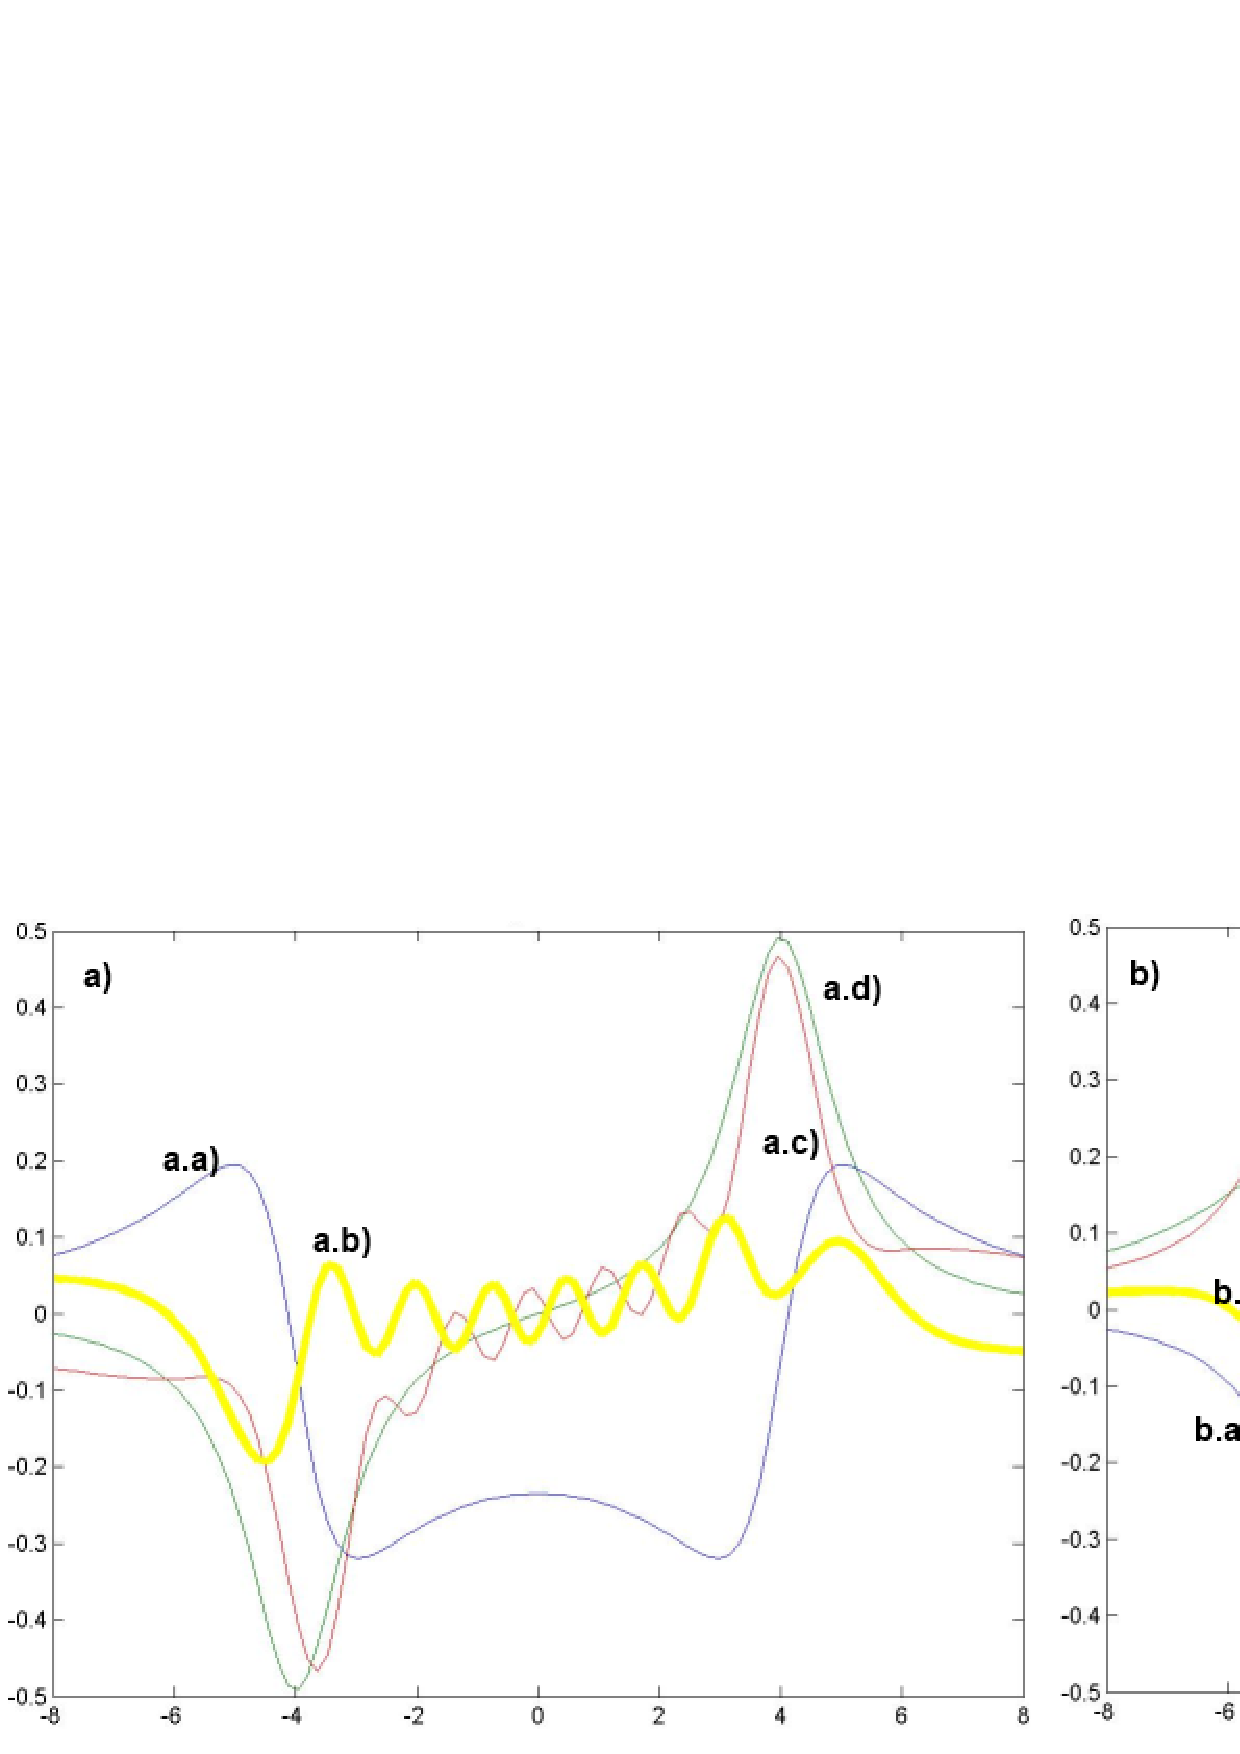
\includegraphics[width=150mm]{img/hht_lin.png}
  \caption{ The Figure presents the results of the Hermite-Hilbert transform method applied to the simple linear model. Results are
  plotted together: 
   a.a) The plot of the real part of $\chi (\omega )$ 
   a.b) absolute error plot (c-plot minus d-plot) 
   a.c) imaginary part of $\chi (\omega )$ obtained with the Hilbert transform of a-plot 
   a.d) imaginary part of $\chi (\omega )$  calculated analytically. 
   b.a) The plot of the imaginary part of $\chi (\omega )$ 
   b.b) absolute error plot (c-plot minus d-plot) 
   b.c) real part of $\chi (\omega )$ obtained with the Hilbert transform of a-plot 
   b.d) real part of $\chi (\omega )$ calculated analytically. \label{fig:hht_lin}
  }
\end{figure}

\subsection{HHT for simple nonlinear model} \label{chap:hermite_nlo}

For the pump-probe and frequency mixing models we have used the same parameters as in Chapter (\ref{chap:nc_nlo}). The results
obtained with the Hermite-Hilbert transform has been presented in Figures (\ref{fig:hht_pnp}) and (\ref{fig:hht_fmix})
respectively.

\begin{figure} 
  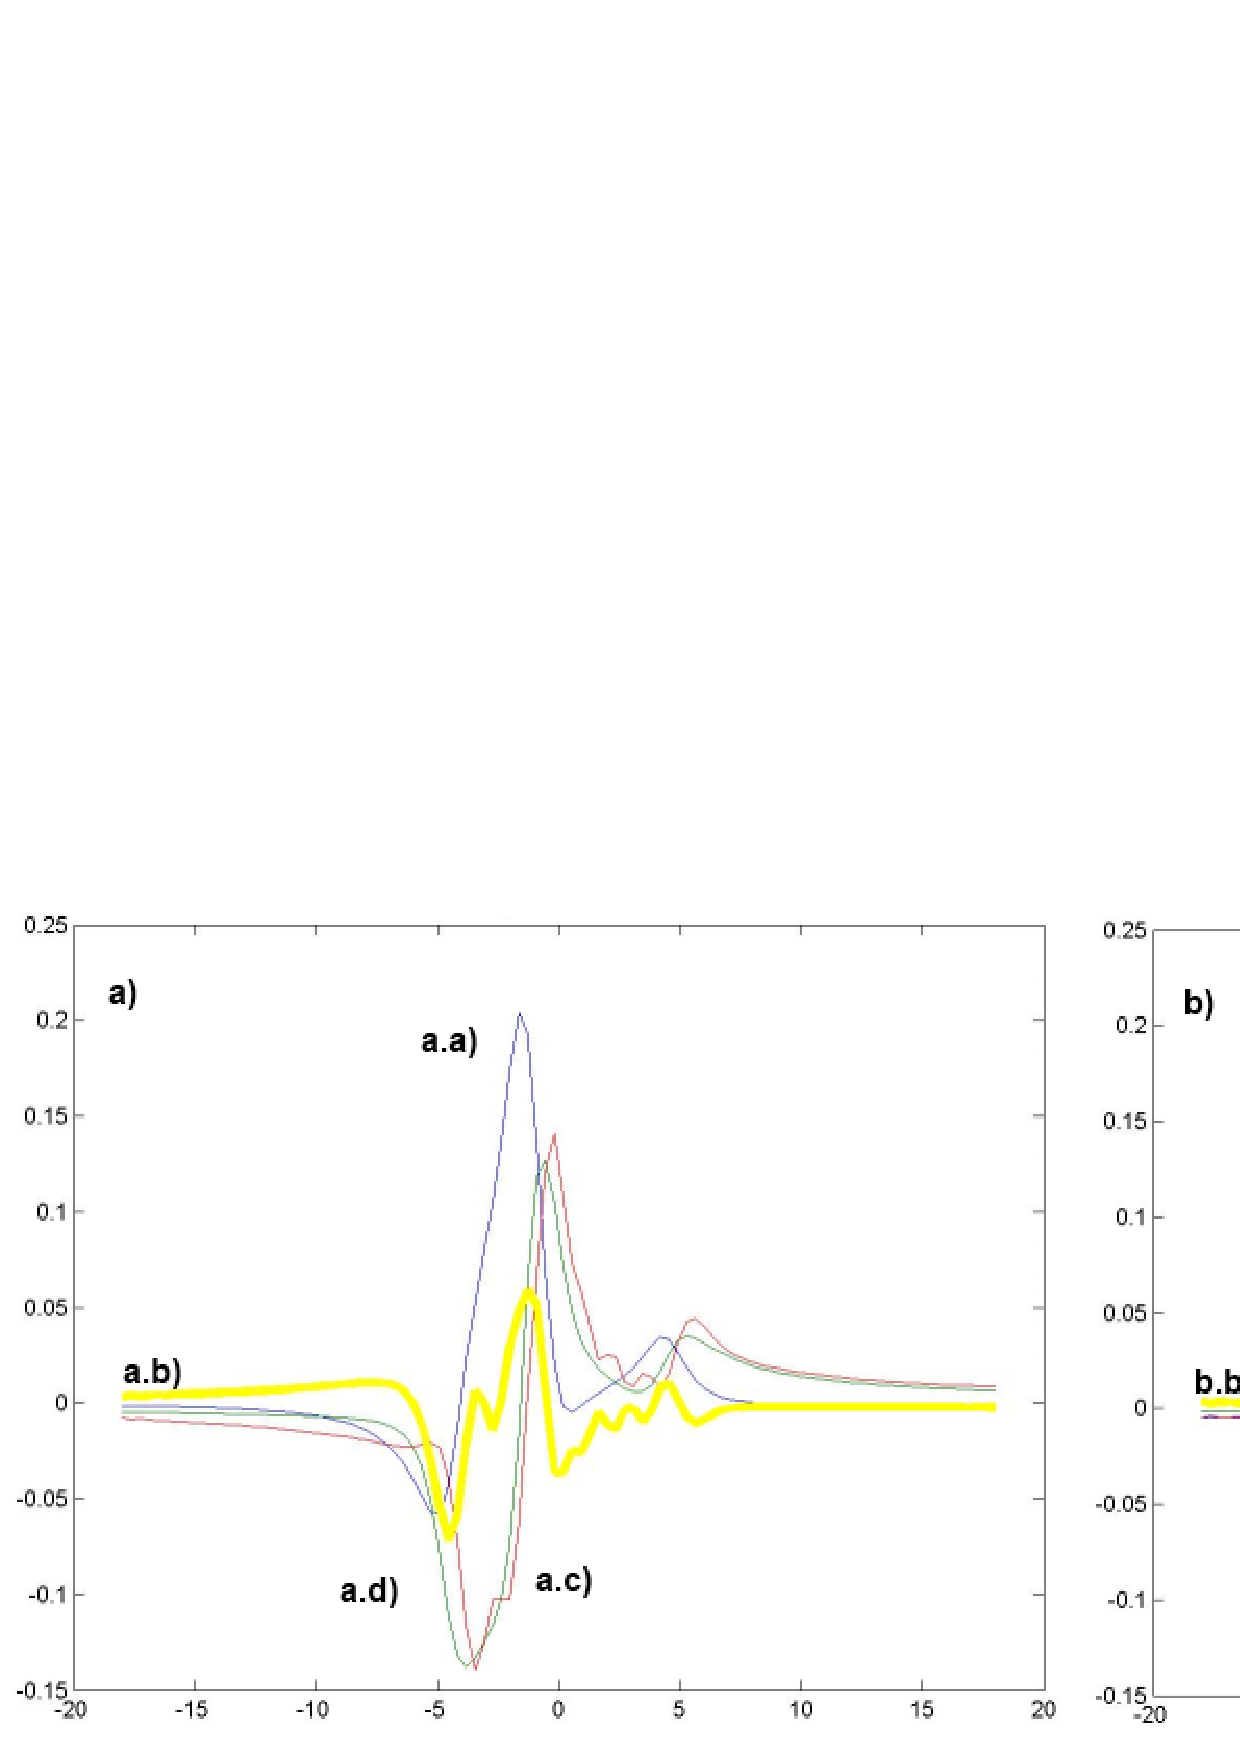
\includegraphics[width=150mm]{img/hht_pnp.png}
  \caption{ The Figure presents the results of the Hermite-Hilbert transform method applied to the pump-and-probe model. Results are
  plotted together: 
     a.a) The plot of the real part of ${\chi_{pp}}(\omega )$
     a.b) absolute error plot (a.d-plot minus a.c-plot)
     a.c) imaginary part of ${\chi_{pp}}(\omega )$ obtained with the Hermite-Hilbert transform of a.a-plot, 
     a.d) imaginary part of ${\chi_{pp}}(\omega )$ calculated analytically 
     b.a) The plot of the imaginary part of ${\chi_{pp}}(\omega )$ 
     b.b) absolute error plot (b.d-plot minus b.c-plot)
     b.c) real part of ${\chi_{pp}}(\omega )$ obtained with the Hermite-Hilbert transform of b.a-plot 
     b.d) real part of $\chi_{pp} (\omega )$ calculated analytically 
     \label{fig:hht_pnp}
     }
\end{figure} 

\begin{figure} 
  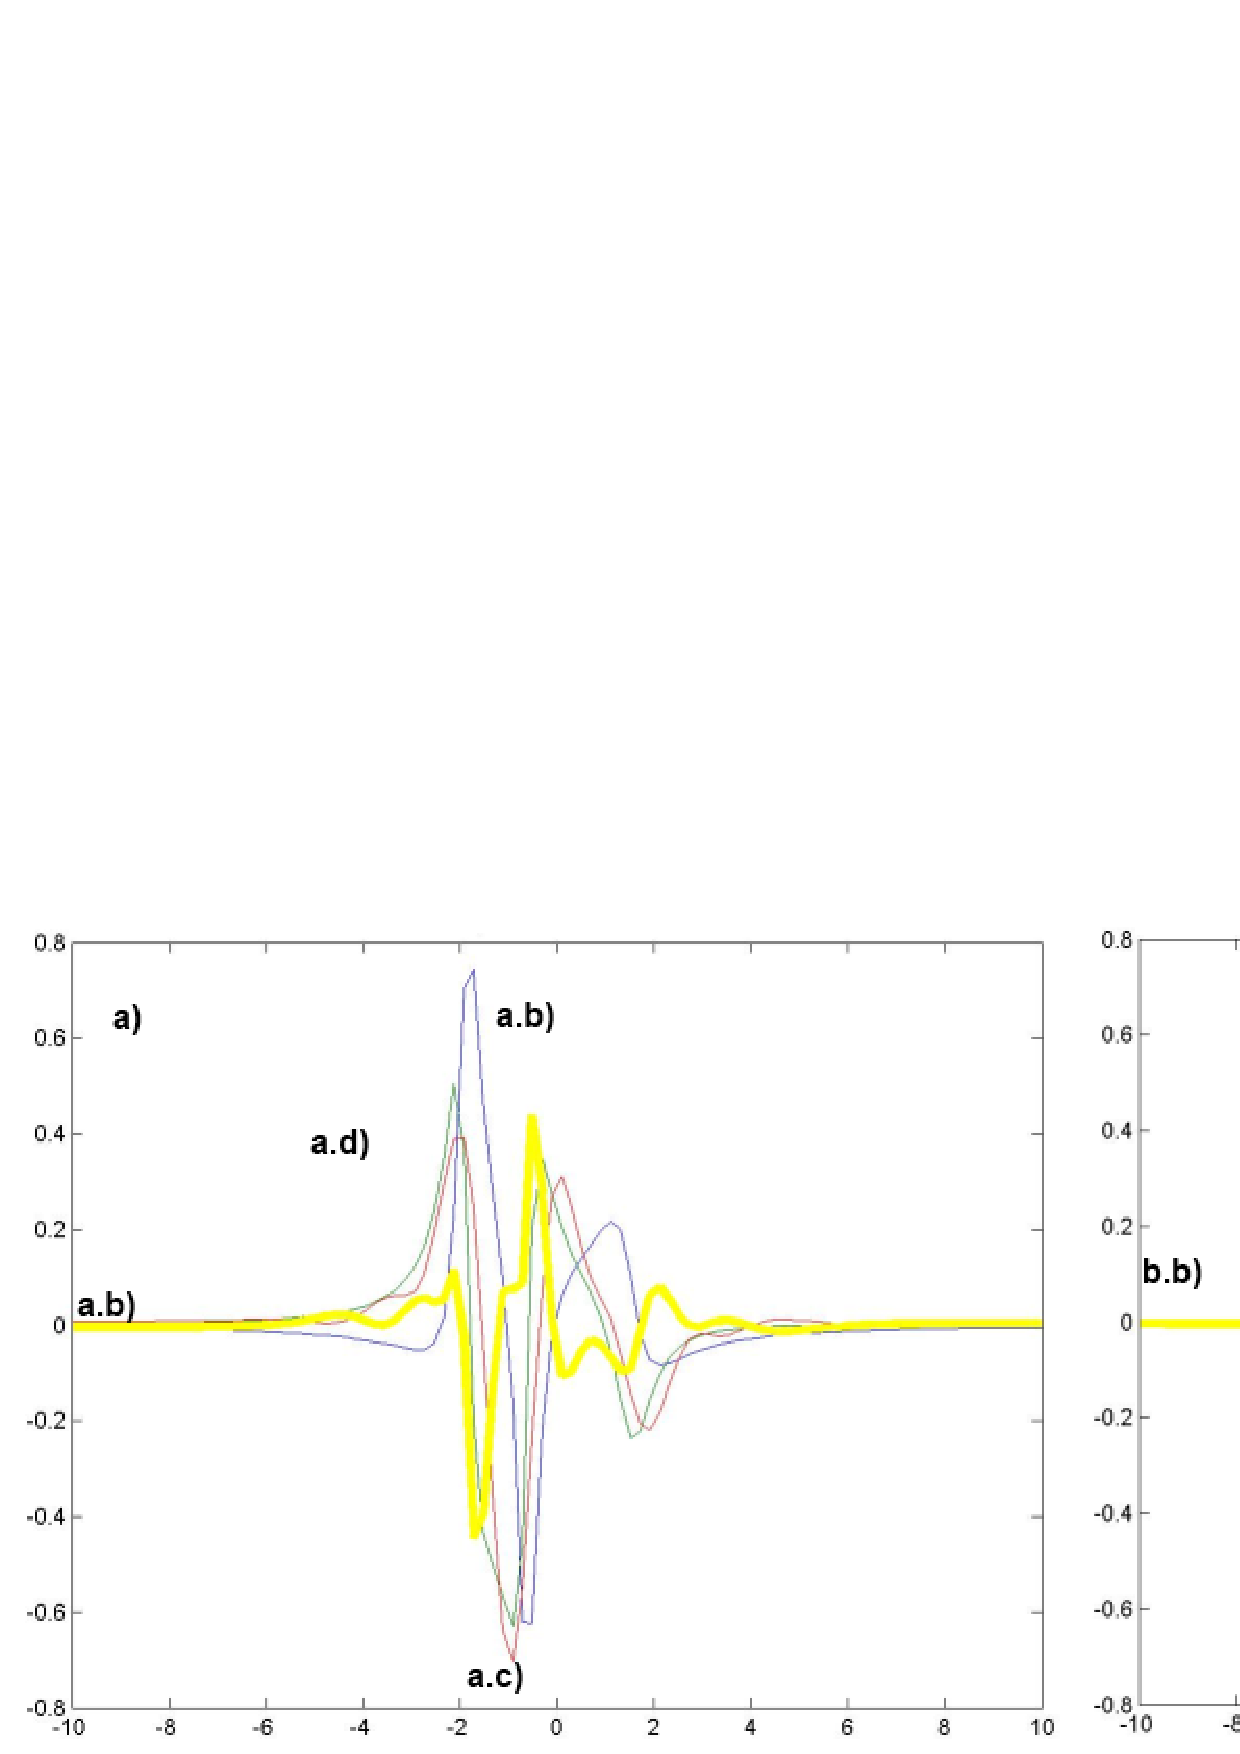
\includegraphics[width=150mm]{img/hht_fmix.png}
  \caption{The Figure presents the results of the Hermite-Hilbert transform method applied to the frequency mixing model. Results are
  plotted together:
     a.a) The plot of the real part of ${\chi_{mix}}(\omega )$
     a.b) absolute error plot (a.d-plot minus a.c-plot)
     a.c) imaginary part of ${\chi_{mix}}(\omega )$ obtained with the Hermite-Hilbert transform of a.a-plot, 
     a.d) imaginary part of ${\chi_{mix}}(\omega )$ calculated analytically 
     b.a) The plot of the imaginary part of ${\chi_{mix}}(\omega )$ 
     b.b) absolute error plot (b.d-plot minus b.c-plot)
     b.c) real part of ${\chi_{mix}}(\omega )$ obtained with the Hermite-Hilbert transform of b.a-plot  
     b.d) real part of $\chi_{mix} (\omega )$ calculated analytically 
     \label{fig:hht_fmix}
     }
\end{figure}

In these results we can draw two conclusions. The method based on the periodical polynomials as Hilbert polynomials will
give us ``zig-zag'' like results. The other conclusion is that results obtained seems to be close, but much worst that those
obtained with HCCI or FHT. 

\subsection{HHT for simple quantum-perturbative model} \label{chap:hermite_quantum}

\subsubsection*{Linear model - results:}

As in the Chapter (\ref{chap:nc_nlo}), we have used the same model to describe the simple linear quantum-perturbative model: 

\begin{equation} \label{eq:hht_qp}
  {\chi_{1, \,qp}}(\omega ) = \frac {N}{\varepsilon_0\,h} \sum_{n=1}^{2}\,(\frac {{\mu_{1, \,n}}\,{ \mu_{2, \,n}}}{{\Omega_{n}}
  - \omega  - i\,{\gamma_{n}}} + \frac {{\mu_{2, \,n}}\,{\mu_{1, \,n}}}{{\Omega_{n}} + \omega + i\,{\gamma_{n}}})
\end{equation}

This time we used the following parameters: \\
$\mu = [[3, \, - 0.5], \,[1.2, \,2.4]]$, 
$\Omega =[ - 3, \,13]$, 
$\gamma =[0.7, \,2.3]$,  
$N=8$, 
${\varepsilon_{0}}=1.4, 
h= - 2.7$

Results are presented in Figure (\ref{fig:hht_qp1}). 

\begin{figure}
  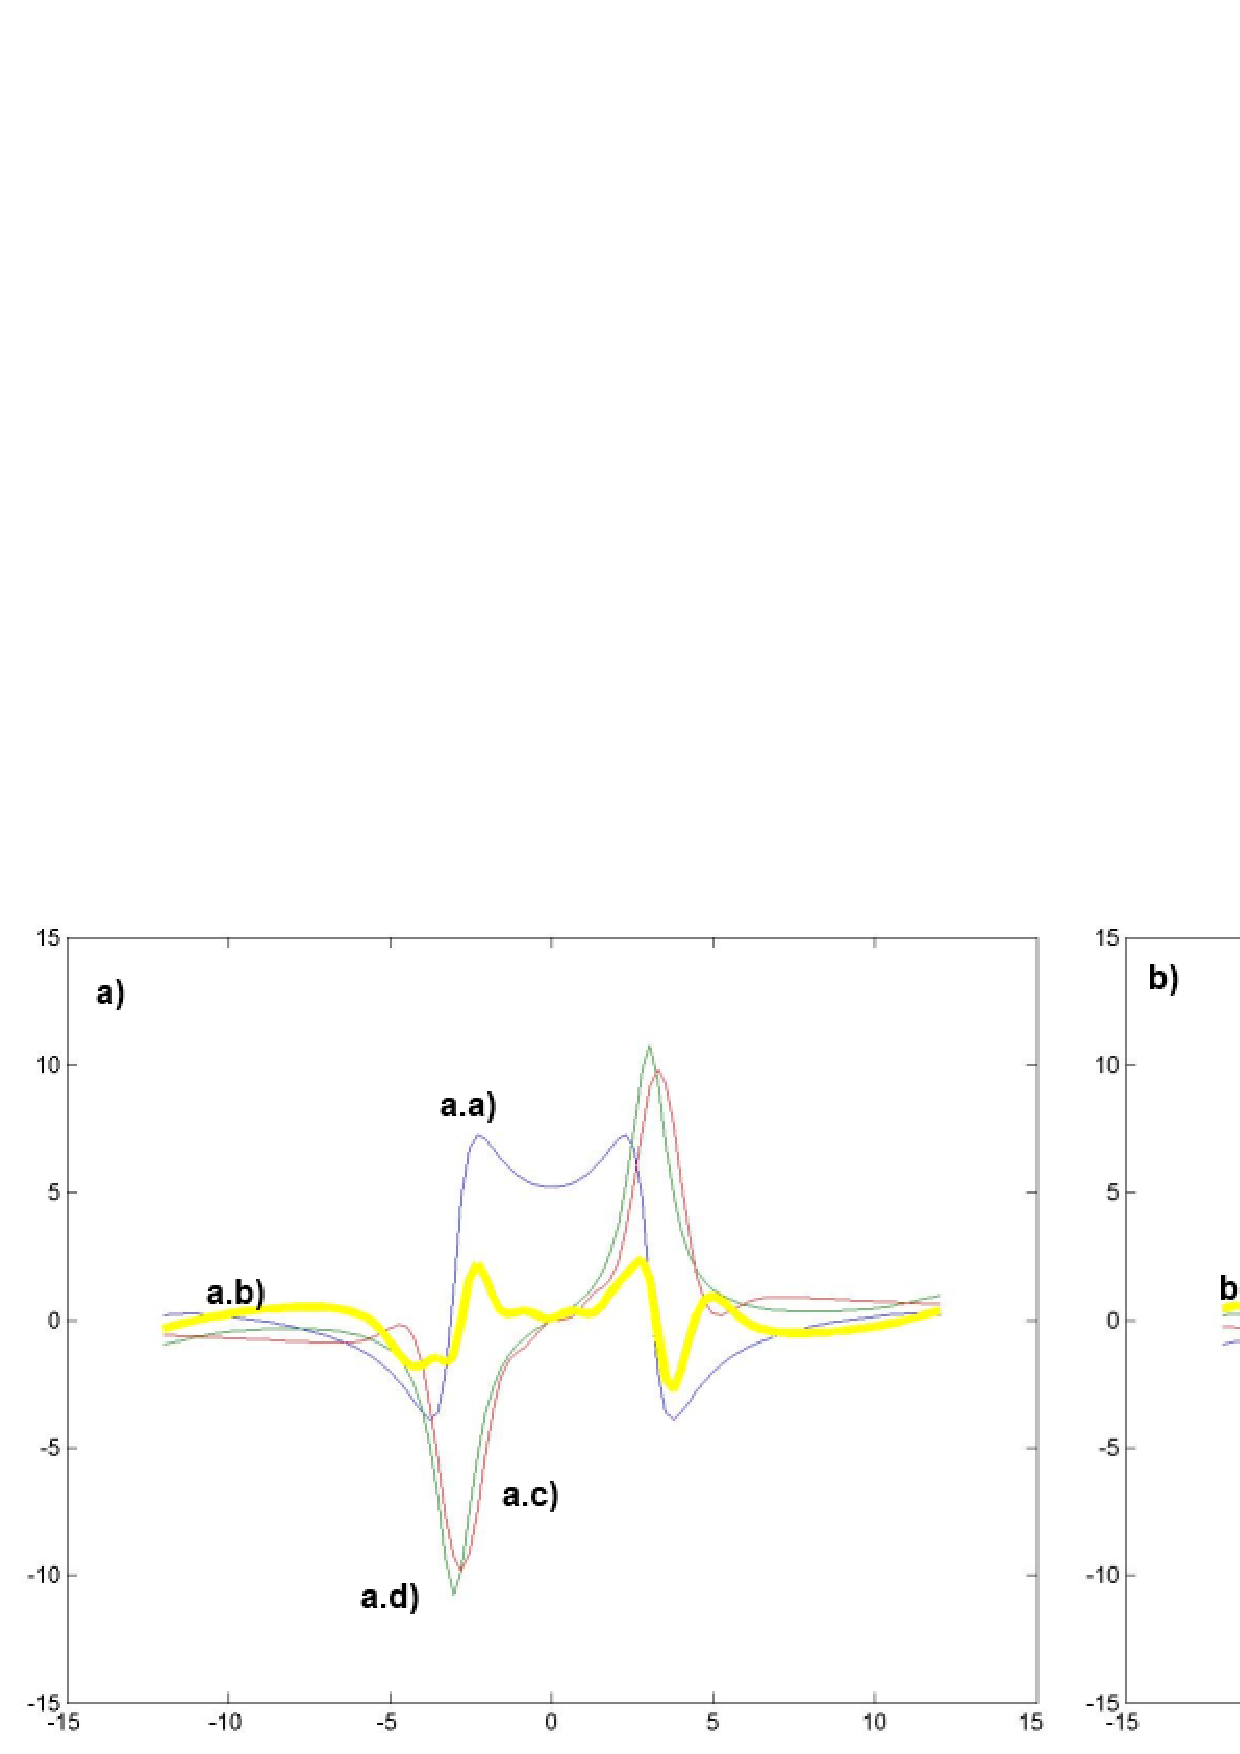
\includegraphics[width=150mm]{img/hht_qp1.png}
  \caption{Results for the linear quantum perturbative model for Hermite-Hilbert transform
    a.a) The plot of the imaginary part of ${\chi_{1, \,qp}}(\omega )$
    a.b) absolute error plot (d-plot minus c-plot) 
    a.c) real part of ${\chi_{1, \, qp}}(\omega )$ obtained with the Hermite-Hilbert transform of a-plot 
    a.d) real part of ${\chi_{1, \, qp}}(\omega )$ calculated analytically 
    b.b) The plot of the real part of ${\chi_{1, \, qp}}(\omega )$ 
    b.b) absolute error plot (d-plot minus c-plot) 
    b.c) imaginary part of ${\chi_{1, \, qp}}(\omega )$ obtained with the Hermite-Hilbert transform of a-plot 
    b.d) imaginary part of ${\chi_{1, \, qp}}(\omega )$ calculated analytically  
    \label{fig:hht_qp1}
  }
\end{figure}

\subsubsection*{Second-order model - results:}

We have also used the same model as in Chapter (\ref{chap:nc_nlo}) to describe the second-order susceptibility model:

\begin{multline} \label{eq:hht_qp2}
  \chi_{2, \,qp}({\omega_{1}}, \,{\omega_{2}}) 
  = 2\, N\,\varepsilon_{0}\,h^{2}\,\sum_{n=1}^{2}\sum_{m=1}^{2}\sum_{l=1}^{2}
  (      \frac {{\mu_{l,\,n}}\,{\mu_{nm}}\,{\mu_{ml}}}
      {({\Omega_{nl}} - \omega_1 - \omega_2 - i\,{\gamma_{nl}})\,({\Omega_{ml}} - \omega_1 - i\,{\gamma_{ml}})} +
  + \\ + \frac   {{\mu_{l, \,n}}\,{\mu_{nm}}\,{\mu_{ml}}}
      {({\Omega_{nl}} - \omega_1 - \omega_1 - i\,{\gamma_{nl}})\,({\Omega_{ml}} - \omega_2 - i\,{\gamma_{ml}})}
  + \\ + \frac   {{\mu_{l, \,n}}\,{\mu_{nm}}\,{\mu_{ml}}}
      {({\Omega_{mn}} - \omega_1 - \omega_2 - i\,{\gamma_{mn}})\,({\Omega_{nl}} + \omega_2 + i\,{\gamma_{nl}})}
  + \\ + \frac{{\mu_{l, \,n }}\,{\mu_{nm}}\,{\mu_{ml}}} 
      {({\Omega_{mn}} - \omega_1 - \omega_2 - i\,{\gamma_{mn}})\,({\Omega_{nl}} + \omega_2 + i\,{\gamma_{nl}})} 
  + \\ + \frac   {{\mu_{l, \,n}}\,{\mu_{nm}}\,{\mu_{ml}}}
      {({\Omega_{nm}} + \omega_1 + \omega_2 + i\,{\gamma_{nm}})\,({\Omega_{ml}} - \omega_1 - i\,{\gamma_{ml}})}
  + \\ + \frac {{\mu_{l, \,n}}\,{\mu_{ nm}}\,{\mu_{ml}}}
      {({\Omega_{nm}} + \omega_1 + \omega_2 + i\,{\gamma_{nm}})\,({\Omega_{ml}} - \omega_1 - i\,{\gamma_{ml}})} 
  + \\ + \frac {{\mu_{l, \,n}}\,{\mu_{nm}}\,{\mu_{ml}}}
      {({\Omega_{ml}} + \omega_1 + \omega_2 + i\,{\gamma_{ml}})\,({\Omega_{nl}} + \omega_1 + i\,{\gamma_{nl}})}
  + \\ + \frac {{\mu_{l, \,n}}\,{\mu_{nm}}\,{\mu_{ml}}}
      {({\Omega_{ml}} + \omega_1 + \omega_2 + i\,{\gamma_{ml}})\,({\Omega_{nl}} + \omega_2 + i\,{\gamma_{nl}})}
  ) ,
\end{multline}
and we will be using the following constants values: \\
$\mu = \left| \begin{array}{cc} 
    1 & 3 \\ -1 & -2 
  \end{array} \right|,\, 
  \Omega = \left| \begin{array}{cc} 
    3 & 16 \\ 4 & 12 
  \end{array} \right|,\,
  \gamma = \left| \begin{array}{cc} 
  1 & 2 \\ -1 & 3
  \end{array} \right|,\, N=5,\, {\varepsilon_{0}}=1,\,h= - 1$

Results are presented in Figure (\ref{fig:hht_qp2}). As for the previous calculations, we can see the model could be invalid
because the occurring errors reach up to 100\%.

\begin{figure} 
  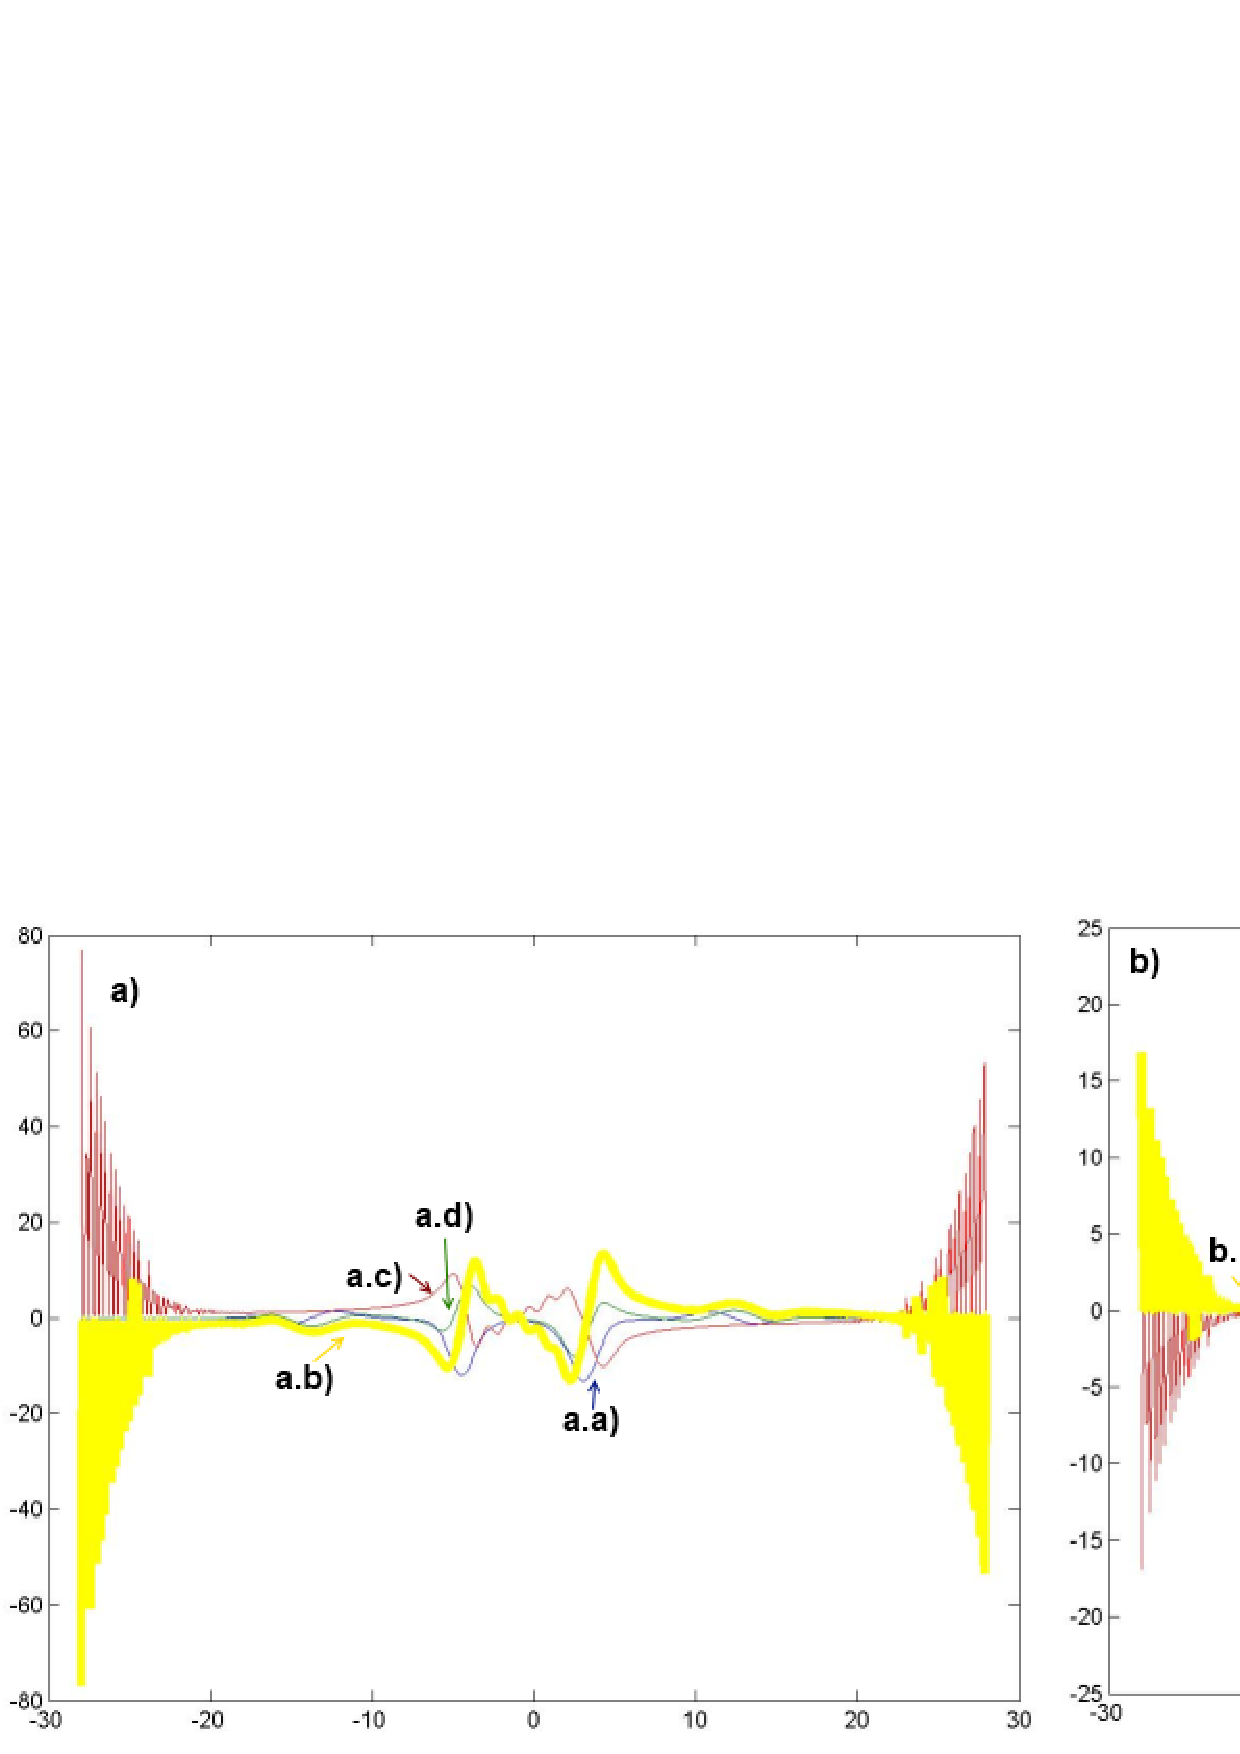
\includegraphics[width=150mm]{img/hht_qp2.png}
  \caption{Results for the second-order quantum perturbative model for Hermite-Hilbert transform transform
     a.a) The plot of the real part of ${\chi_{2, \,qp}}(\omega )$
     a.b) absolute error plot (a.d-plot minus a.c-plot)
     a.c) imaginary part of ${\chi_{2, \,qp}}(\omega )$ obtained with the Hermite-Hilbert transformof a.a-plot, 
     a.d) imaginary part of ${\chi_{2, \,qp}}(\omega )$ calculated analytically 
     b.a) The plot of the imaginary part of ${\chi_{2, \,qp}}(\omega )$ 
     b.b) absolute error plot (b.d-plot minus b.c-plot)
     b.c) real part of ${\chi_{2, \,qp}}(\omega )$ obtained with the Hermite-Hilbert transform of b.a-plot 
     b.d) real part of $\chi_{2, \,qp} (\omega )$ calculated analytically 
     \label{fig:hht_qp2}
     }
\end{figure} 

We have checked the HHT method for various parameters, but none of them has gave us better accuracy. We
encourage the reader to carry out their own calculations with source code given in Appendix A.5.

\section{Fourier-series} \label{chap:fourier}

\subsection{Overview of the Fourier-series based method}  \label{chap:fourier_overview}

The concept of the Hilbert transform evaluation based on the Fourier series also comes from the master thesis by Mathias Johansson
\cite{johansson_hilbert}. There is an important drawback in this approach - in general it should be applied to the periodical
functions, but we will further assume they have a relatively long period. 

\subsubsection*{Fourier series:} 

Each periodical function can be decomposed into a infinite Fourier series. For a given periodic function f with a given period 2*P,
we will introduce the Fourier coefficients:

\begin{subequations} \label{eq:fourier_coeffs}
  \begin{equation}   \label{eq:fcoeffs_an}
    {a_{f, \,n}}=\int_{ - P}^{P}\mathrm{f}(x)\,\mathrm{cos}(n\,x)\, dx
  \end{equation}
  \begin{equation}   \label{eq:fcoeffs_bn}
    {b_{f, \,n}}=\int_{ - P}^{P}\mathrm{f}(x)\,\mathrm{sin}(n\,x)\, dx
  \end{equation}
\end{subequations}

Not getting deeply into harmonic analysis - we will assume that a series of partial sums:

\begin{equation} \label{eq:fourier_partialsums}
  {S_{f, \,N}}(x)=\frac {{a_{f, \,0}}}{2} + (\sum_{n=1}^{N}\,({a
_{f, \,n}}\,\mathrm{cos}(n\,x) + {b_{f, \,n}}\,\mathrm{sin}(n\,x)
))
\end{equation}

for a function $f\,\ \in \,{L_{2}}( - P, \,P)$ converges at almost every point to the f, which can be written as:

\begin{equation} \label{eq:fourier_canbewritten}
  \mbox{if }\,S = \{t : \lim_{N\rightarrow \infty }\,{S_{f, \,N}}(t) \neq \mathrm{f}(t) \} then |S| \leq {\aleph_{0}}
\end{equation}

\subsubsection*{Hilbert transform based on the Fourier series:}

After Johansson \cite{johansson_hilbert} we state that for any given function $f\,\ \textbf{in}\ \,{L_{2}}( - P, \,P)$ we can
calculate the Hilbert transform using the form of Fourier series for this function. All we need to do, is to make a swap in the
(\ref{eq:fourier_partialsums}) equation - the ${a_{n}}$ coefficients should be swapped with ${b_{n}}$ coefficients.

\begin{multline} \label{eq:fourier_hilbert}
  HILBERT(f(x)) = \lim_{N\rightarrow \infty }\,\frac {{a_{f, \,0}}}{2} 
  + \\ + (\sum_{ n=1}^{N}\,({b_{f, \,n}}\,\mathrm{cos}(n\,x)
       + {a_{f, \,n}}\, \mathrm{sin}(n\,x)))
       \,\mbox{ [at alm. every point x] }
\end{multline}

\subsubsection*{Algorithm overview:}

As mentioned before, we will prepare the algorithm as for the periodic function, but we will try to imply that the period is much longer
than the area of interest. We would like to calculate the Hilbert transform for periodical and non-periodical function f. The first step is
to calculate the properties of the input X interval, which is the region in which we are interested of both input function f values and the
values of its Hilbert transform. The second step is to calculate the Fourier coefficients in a main loop. In the same loop we calculate the
next partial sum values. The last step is to extract the inner interval from the extended interval, to omit the numerical errors near the
interval edges.

The full source code of this algorithm, has been presented in the appendix A.6.

\subsection{Fourier-series for simple linear model} \label{chap:fourier_lin}

In Figure (\ref{fig:four_lin}) we have presented the results obtained with the Fourier-Hilbert transform for the simple
linear model defined in model (\ref{eq:physical_frequency_linear}). As we can see - the Fourier-Hilbert transform comes with poor accuracy,
but we would like to put this method into examination with defined models.

\begin{figure} 
  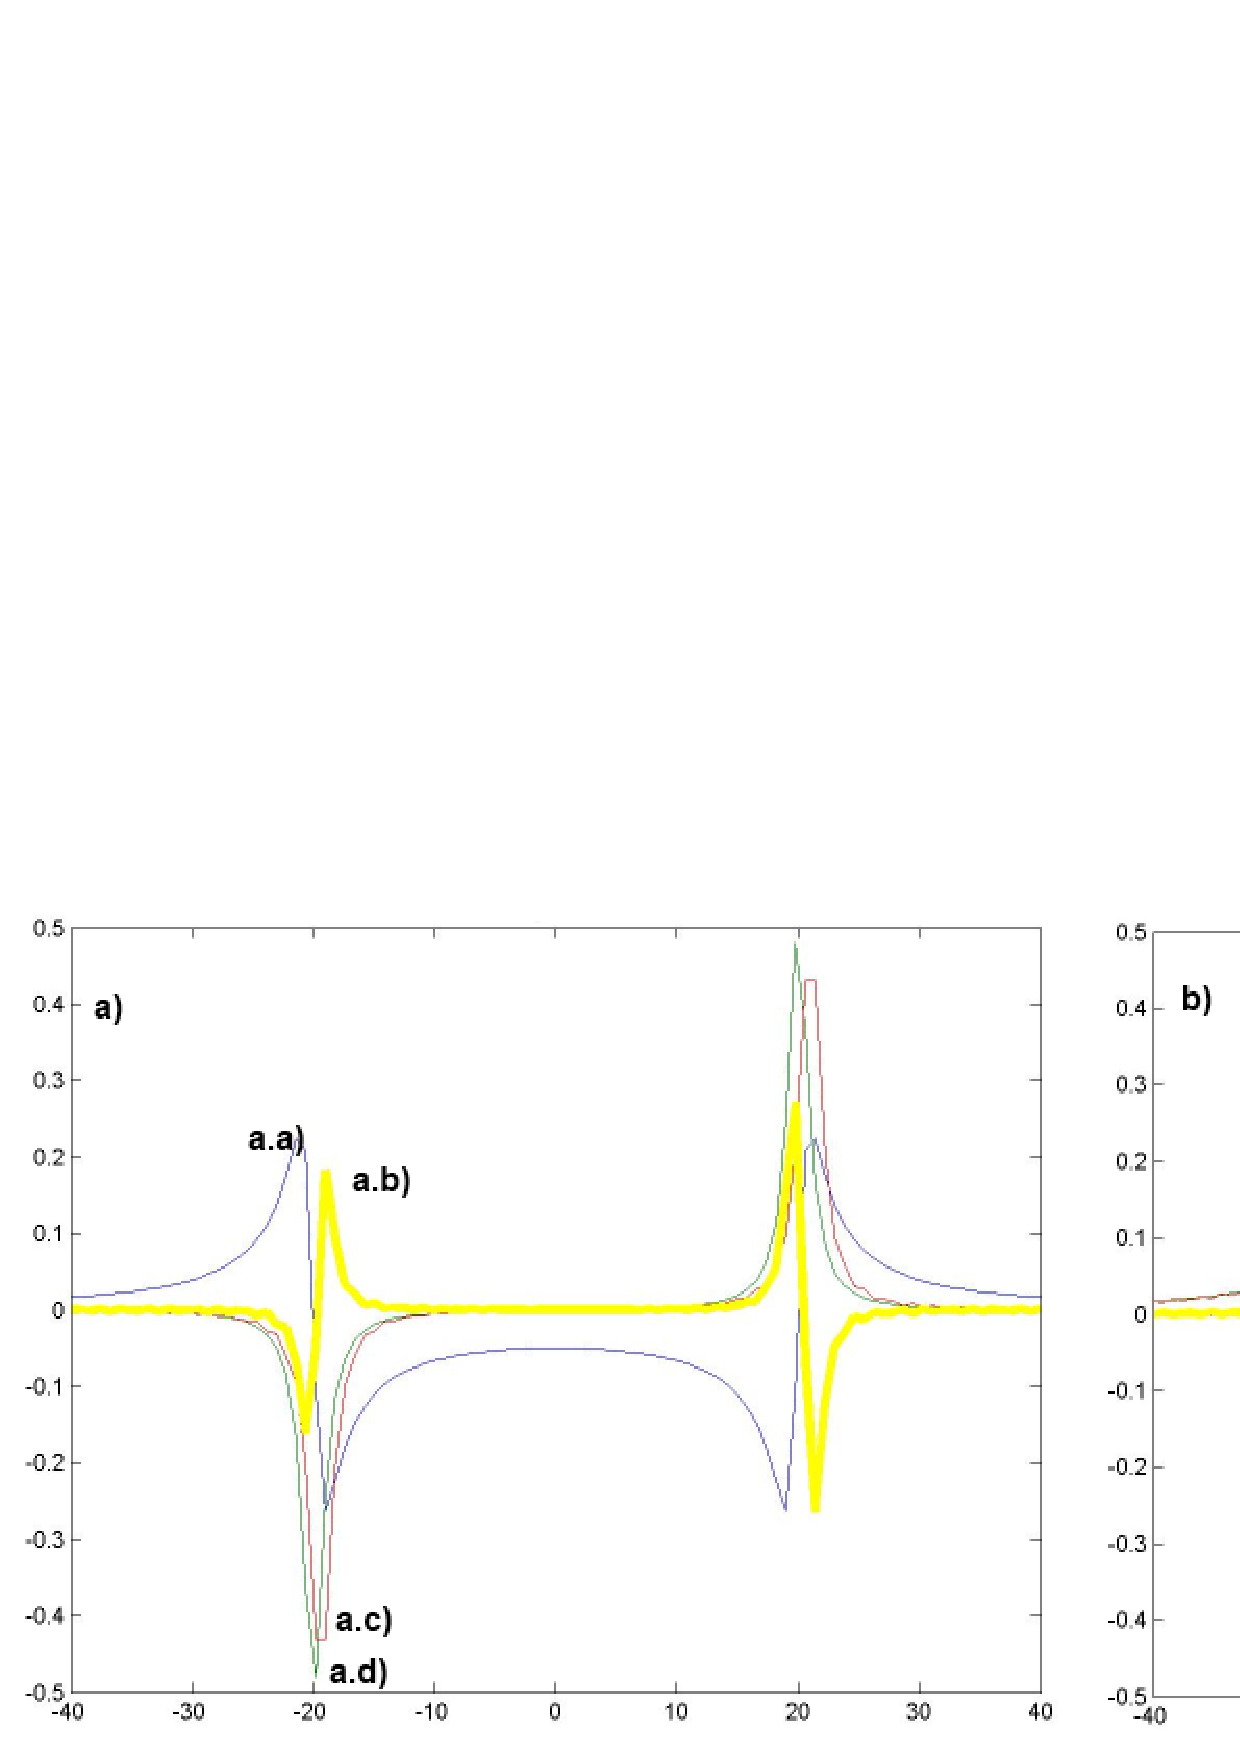
\includegraphics[width=150mm]{img/four_lin.png}
  \caption{ The Figure presents the results of the Hilbert transform based on the Fourier series method applied to the simple linear model.
  Results are plotted together:
   a.a) The plot of the real part of $\chi (\omega )$ 
   a.b) absolute error plot (c-plot minus d-plot) 
   a.c) imaginary part of $\chi (\omega )$ obtained with the Fourier-Hilbert transform of a-plot 
   a.d) imaginary part of $\chi (\omega )$  calculated analytically. 
   b.a) The plot of the imaginary part of $\chi (\omega )$ 
   b.b) absolute error plot (c-plot minus d-plot) 
   b.c) real part of $\chi (\omega )$ obtained with the Fourier-Hilbert transform of a-plot 
   b.d) real part of $\chi (\omega )$ calculated analytically. \label{fig:four_lin}
  }
\end{figure} 

\subsection{Fourier-series for simple nonlinear model} \label{chap:fourier_nlo}

For the pump-probe and frequency mixing models we have used the same parameters as in Chapter (\ref{chap:nc_nlo}). The results
obtained with the Fourier-Hilbert transform has been presented in Figures (\ref{fig:four_pnp}) and (\ref{fig:four_fmix})
respectively.

\begin{figure} 
  \includegraphics[width=150mm]{img/four_pnp.png}
  \caption{The Figure presents the results of the Hilbert transform based on the Fourier series method applied to the pump-and-probe model.
  Results are plotted together:
     a.a) The plot of the real part of ${\chi_{pp}}(\delta )$
     a.b) absolute error plot (a.d-plot minus a.c-plot)
     a.c) imaginary part of ${\chi_{pp}}(\delta )$ obtained with the Fourier-Hilbert transform of a.a-plot, 
     a.d) imaginary part of ${\chi_{pp}}(\delta )$ calculated analytically 
     b.a) The plot of the imaginary part of ${\chi_{pp}}(\delta )$ 
     b.b) absolute error plot (b.d-plot minus b.c-plot)
     b.c) real part of ${\chi_{pp}}(\delta )$ obtained with the Fourier-Hilbert transform of b.a-plot 
     b.d) real part of $\chi_{pp} (\omega )$ calculated analytically 
     \label{fig:four_pnp}
     }
\end{figure} 

\begin{figure} 
  \includegraphics[width=150mm]{img/four_fmix.png}
  \caption{ The Figure presents the results of the Hilbert transform based on the Fourier series method applied to the frequency mixing
  model. Results are plotted together:
     a.a) The plot of the real part of ${\chi_{mix}}(\omega )$
     a.b) absolute error plot (a.d-plot minus a.c-plot)
     a.c) imaginary part of ${\chi_{mix}}(\omega )$ obtained with the Fourier-Hilbert transform of a.a-plot, 
     a.d) imaginary part of ${\chi_{mix}}(\omega )$ calculated analytically 
     b.a) The plot of the imaginary part of ${\chi_{mix}}(\omega )$ 
     b.b) absolute error plot (b.d-plot minus b.c-plot)
     b.c) real part of ${\chi_{mix}}(\omega )$ obtained with the Fourier-Hilbert transform of b.a-plot  
     b.d) real part of $\chi_{mix} (\omega )$ calculated analytically 
     \label{fig:four_fmix}
     }
\end{figure}

In these results we can draw two conclusions. The method based on the periodical polynomials as Fourier series will
give us ``zig-zag'' like results. The other conclusion is that results obtained seems to be close, but much worst that those
obtained with HCCI or FHT. 

\subsection{Fourier-series for simple quantum-perturbative model} \label{chap:fourier_quantum}

\subsubsection*{Linear model - results:}

As in the Chapter (\ref{chap:nc_nlo}), we have used the same model to describe the simple linear quantum-perturbative model: 

\begin{equation} \label{eq:four_qp}
  {\chi_{1, \,qp}}(\omega ) = \frac {N}{\varepsilon_0\,h} \sum_{n=1}^{2}\,(\frac {{\mu_{1, \,n}}\,{ \mu_{2, \,n}}}{{\Omega_{n}}
  - \omega  - i\,{\gamma_{n}}} + \frac {{\mu_{2, \,n}}\,{\mu_{1, \,n}}}{{\Omega_{n}} + \omega + i\,{\gamma_{n}}})
\end{equation}

This time we used the following parameters: \\
$\mu = [[3, \, - 0.5], \,[1.2, \,2.4]]$, 
$\Omega =[ - 3, \,13]$, 
$\gamma =[0.7, \,2.3]$,  
$N=8$, 
${\varepsilon_{0}}=1.4$, 
$h= - 2.7$.

Results are presented in Figure (\ref{fig:four_qp1}). 

\begin{figure}
  \includegraphics[width=150mm]{img/four_qp1.png}
  \caption{Results for the linear quantum perturbative model for Fourier-Hilbert transform
    a.a) The plot of the imaginary part of ${\chi_{1, \, qp}}(\omega )$
    a.b) absolute error plot (d-plot minus c-plot) 
    a.c) real part of ${\chi_{1, \, qp}}(\omega )$ obtained with the Fourier-Hilbert transform of a-plot 
    a.d) real part of ${\chi_{1, \, qp}}(\omega )$ calculated analytically 
    b.b) The plot of the real part of ${\chi_{1, \, qp}}(\omega )$ 
    b.b) absolute error plot (d-plot minus c-plot) 
    b.c) imaginary part of ${\chi_{1, \, qp}}(\omega )$ obtained with the Fourier-Hilbert transform of a-plot 
    b.d) imaginary part of ${\chi_{1, \, qp}}(\omega )$ calculated analytically  
    \label{fig:four_qp1}
  }
\end{figure}

\subsubsection*{Second-order model - results:}

We have also used the same model as in Chapter (\ref{chap:nc_nlo}) to describe the second-order susceptibility model:

\begin{multline} \label{eq:four_qp2}
  \chi_{2, \,qp}({\omega_{1}}, \,{\omega_{2}}) = 
   2\,N\,\varepsilon_{0}\,h^{2}\sum_{n=1}^{2}\sum_{m=1}^{2}\sum_{l=1}^{2}\,
  (      \frac {{\mu_{l,\,n}}\,{\mu_{nm}}\,{\mu_{ml}}}
      {({\Omega_{nl}} - \omega_1 - \omega_2 - i\,{\gamma_{nl}})\,({\Omega_{ml}} - \omega_1 - i\,{\gamma_{ml}})} 
  + \\ + \frac {{\mu_{l, \,n}}\,{\mu_{nm}}\,{\mu_{ml}}}
      {({\Omega_{nl}} - \omega_1 - \omega_1 - i\,{\gamma_{nl}})\,({\Omega_{ml}} - \omega_2 - i\,{\gamma_{ml}})}
  + \\ + \frac {{\mu_{l, \,n}}\,{\mu_{nm}}\,{\mu_{ml}}}
      {({\Omega_{mn}} - \omega_1 - \omega_2 - i\,{\gamma_{mn}})\,({\Omega_{nl}} + \omega_2 + i\,{\gamma_{nl}})}
  + \\ + \frac{{\mu_{l, \,n }}\,{\mu_{nm}}\,{\mu_{ml}}} 
      {({\Omega_{mn}} - \omega_1 - \omega_2 - i\,{\gamma_{mn}})\,({\Omega_{nl}} + \omega_2 + i\,{\gamma_{nl}})} 
  + \\ + \frac {{\mu_{l, \,n}}\,{\mu_{nm}}\,{\mu_{ml}}}
      {({\Omega_{nm}} + \omega_1 + \omega_2 + i\,{\gamma_{nm}})\,({\Omega_{ml}} - \omega_1 - i\,{\gamma_{ml}})}
  + \\ + \frac {{\mu_{l, \,n}}\,{\mu_{ nm}}\,{\mu_{ml}}}
      {({\Omega_{nm}} + \omega_1 + \omega_2 + i\,{\gamma_{nm}})\,({\Omega_{ml}} - \omega_1 - i\,{\gamma_{ml}})} 
  + \\ + \frac {{\mu_{l, \,n}}\,{\mu_{nm}}\,{\mu_{ml}}}
      {({\Omega_{ml}} + \omega_1 + \omega_2 + i\,{\gamma_{ml}})\,({\Omega_{nl}} + \omega_1 + i\,{\gamma_{nl}})}
  + \\ + \frac {{\mu_{l, \,n}}\,{\mu_{nm}}\,{\mu_{ml}}}
      {({\Omega_{ml}} + \omega_1 + \omega_2 + i\,{\gamma_{ml}})\,({\Omega_{nl}} + \omega_2 + i\,{\gamma_{nl}})}
  ) ,
\end{multline}
and we will be using the following constants values:
$\mu = \left| \begin{array}{cc} 
    1 & 3 \\ -1 & -2 
  \end{array} \right|,\, 
  \Omega = \left| \begin{array}{cc} 
    3 & 16 \\ 4 & 12 
  \end{array} \right|,\,
  \gamma = \left| \begin{array}{cc} 
  1 & 2 \\ -1 & 3
  \end{array} \right|,\, N=5,\, {\varepsilon_{0}}=1,\,h= - 1$ .

Results are presented in Figure (\ref{fig:four_qp2}). We can see, that the first model could be valid, while the second model seems to
be invalid for consecutively for all Hilbert transform implementations.

\begin{figure} 
  \includegraphics[width=150mm]{img/four_qp2.png}
  \caption{Results for the second-order quantum perturbative model for Fourier-Hilbert transform transform
     a.a) The plot of the real part of ${\chi_{2, \,qp}}(\omega )$
     a.b) absolute error plot (a.d-plot minus a.c-plot)
     a.c) imaginary part of $\chi_{2, \, qp} (\omega )$ obtained with the Fourier-Hilbert transformof a.a-plot, 
     a.d) imaginary part of $\chi_{2, \, qp} (\omega )$ calculated analytically 
     b.a) The plot of the imaginary part of ${\chi_{2, \, qp}}(\omega )$ 
     b.b) absolute error plot (b.d-plot minus b.c-plot)
     b.c) real part of $\chi_{2, \, qp} (\omega )$ obtained with the Fourier-Hilbert transform of b.a-plot 
     b.d) real part of $\chi_{2, \, qp} (\omega )$ calculated analytically 
     \label{fig:four_qp2}
     }
\end{figure} 

We have checked the Fourier-Hilbert method for various parameters, but none of them has gave us better accuracy. We
encourage the reader to carry out their own calculations with source code given in Appendix A.6.

\section{MATLAB ® out-of-the-box functions} \label{chap:matlab}

\subsection{Overview of the MATLAB ® interior functions} \label{chap:matlab_overview}

Why not take into consideration the already built-in numerical methods from MATLAB? We compare the results obtained with: 


\begin{tabular}{l l}
  - quadgk() &- adaptive Gauss-Kronrod quadrature; \\
  - hilbert() &- fast Hilbert transform based on both FFT and IFFT. \\
\end{tabular}


\subsubsection*{Adaptive Gauss-Kronrod quadrature - theory:}

The source code of the adaptive Gauss-Kronrod quadrature has been published in the popular Fortran 77 numerical integration
QUADPACK library and has been also translated into the MATLAB core language. It is also based on the ''quadva'' routine described by
Lawrence F. Shampine in \cite{shampine_vectorized}. The fundamental idea of this numerical integration algorithm is the nested
quadrature rule - the more accurate quadrature approximation is calculated from the less accurate one. The algorithm is adaptive
and the error estimation is based on the (G-K7,15) pair of the quadrature rules - less and more accurate - the 7-point Gauss rule
and the 15-point Kronrod rule with a share nodes. For more information about the theory beneath this algorithm - please read D.
Calvetti et al \cite{calvetti_computation} or the chapter 5.5 from the book by David Kahaner \cite{kahaner_numerical}.

\subsubsection*{Adaptive Gauss-Kronrod quadrature - short tutorial:}

We have used the MATLAB \textregistered R2009b. It comes with built-in quadgk function with four parameters:


\begin{tabular}{l l}
  'AbsTol'           & - absolute error tolerance \\
  'RelTol'           & - relative error tolerance \\
  'Waypoints'        & - vector of integration waypoints \\
  'MaxIntervalCount' & - maximum number of intervals allowed (default: 650) \\
\end{tabular}

The defined models used within the Hilbert transform comes with one, but strong singularity. While the quadgk() method comes with
copes with infinities, we have suggested to split the integral into two parts, but not including the small area nearby singularity.

If the models singularity $c$ is taken from the range $[a, b]$, we will divide the range $|b-a|$ by $10000$ and calculate the value
as defined in equation (\ref{eq:mat_quadadd}). 
 
\begin{alignat}{1} \label{eq:mat_quadadd}
  \dashint_{ - \infty }^{\infty } \frac {f(x)}{x-c} \, dx \approx 
          & \, quadgk(\frac {f(x)}{x-c}, - \infty, c - \frac{|b-a|}{10000}, \text{'RelTol'}, 0.001, \text{'AbsTol'}, 0.001 ) \\
     + \, & \, quadgk(\frac {f(x)}{x-c}, c + \frac{|b-a|}{10000}, + \infty, \text{'RelTol'}, 0.001, \text{'AbsTol'}, 0.001 )
     \nonumber
\end{alignat}
 
\subsubsection*{Fast Hilbert transform routine - theory:}

The discrete Hilbert transform (DHT) is given by definition after \cite{kak_multilayeredarray} - for a given n-length X vector:

\begin{equation} \label{eq:matlab_fhttheroy}
  \mathrm{DHT}({X_{k}})=\frac {1}{n} \left(  \! \sum_{s=0}^{n - 1}\,{X _{s}}\,(1 - ( - 1)^{(k - s)})\,\mathrm{cot}(\frac {\pi \,(k
  - s) }{n}) \!  \right) 
\end{equation}

The other definition by \cite{calvetti_computation} uses the convolution:

\begin{subequations} \label{eq:matlab_convolution}
  \begin{equation}   \label{eq:mconv_dht}
    \mathrm{DHT}({X_{k}})  = X[] * h[] = \sum_{s=0}^{n - 1}\,{h_{k - s}}\,{X_{s}}
  \end{equation}
  \begin{equation}   \label{eq:mconv_hk}
    {h_{k}}=\frac {1}{n} \left(  \! \mathrm{cot}(\frac {\pi \,k}{n}) - \frac {\mathrm{cos}(\pi \,k)}{\mathrm{sin}(\frac {\pi
    \,k}{n})}\! \right) 
  \end{equation}
\end{subequations}

The important issue is that the DHT is closely related to the discrete Fourier transform (DFT). For a given n-length X vector in
order to evaluate the DHT(X) we can hire the DFT routine. To start, we must remember that in the continuous case:

\begin{equation} \label{eq:matlab_issue}
  \mathrm{FOURIER}(\mathrm{HILBERT}(X_k))=( - i\,\mathrm{sgn}( \frac {n}{2} - k)\,\mathrm{sgn}(k))\,\mathrm{FOURIER}({X_{k}}),
\end{equation}

where we remember that:

\begin{equation} \label{eq:matlab_kernel}
   - i\,\mathrm{sgn}(\frac {n}{2} - k)\,\mathrm{sgn}(k)=\mathrm{FOURIER}(\frac {1}{\pi \,k}) .
\end{equation}

Therefore, in the discrete case we find the similar equation to (\ref{eq:matlab_issue}) relating the DHT and DFT:

\begin{equation} \label{eq:matlab_reldhtdft}
  \mathrm{DFT}(\mathrm{DHT}({X_{k}}))=( - i)\,\mathrm{sgn}(\frac {n}{2} - k)\,\mathrm{sgn}(k)\,\mathrm{DFT}({X_{k}})
\end{equation}

From the (\ref{eq:matlab_reldhtdft}) we can see, that it is quite easy to operate within the Fourier/frequency domain - because the
quite complicate convolution is transformed to a simple algebraic operations. Also - if we have the quick algorithm to perform both
the DFT and inverse-DFT - for example with the fast Fourier transform (FFT) and the inverse fast Fourier transform (IFFT) - the DHT
operation will be calculated as follows:

\begin{equation} \label{eq:matlab_fulldhthdf}
  \mathrm{DHT}({X_{k}})=\mathrm{IDFT}(( - i)\,\mathrm{sgn}(\frac {n}{2} - k)\,\mathrm{sgn}(k)\,\mathrm{DFT}({X_{k}}))
\end{equation}

\subsubsection*{Fast Hilbert transform routine - short tutorial:}

While the hired DFT and IDFT routines are evaluated in complex domain, for a given input n-length X vector we have that:

\begin{equation} \label{eq:matlab_implication}
  \mathrm{hilbert}(X) \Rightarrow X + i\,\mathrm{DHT}(X)
\end{equation}

In order to obtain the final result we need to take the imaginary part of the MATLAB hilbert() function output. The other
important issue is that the \textit{MATLAB®} hilbert() function has one optional parameter called N - to computer the N-point
Hilbert transform. If the input vector X is too short, it will be padded with zeros, otherwise it will be truncated. 

\subsection{MIF for simple linear model} \label{chap:matlab_lin}

In two Figures (\ref{fig:quadgk_lin}) and (\ref{fig:hilb_lin}) we have ga\-thered the results ob\-tained with the MATLAB quadgk() and
hilbert() functions based Hil\-bert trans\-forms for the simple linear model defined in model (\ref{eq:physical_frequency_linear}).
For each method we can see a accep\-table accu\-racy.

\begin{figure} 
  \includegraphics[width=150mm]{img/quadgk_lin.png}
  \caption{The Figure presents the results of the quadgk() method applied to the simple linear model. Results are plotted together:
   a.a) The plot of the real part of $\chi (\omega )$ 
   a.b) absolute error plot (c-plot minus d-plot) 
   a.c) imaginary part of $\chi (\omega )$ obtained with the quadgk()-Hilbert transform of a-plot 
   a.d) imaginary part of $\chi (\omega )$  calculated analytically. 
   b.a) The plot of the imaginary part of $\chi (\omega )$ 
   b.b) absolute error plot (c-plot minus d-plot) 
   b.c) real part of $\chi (\omega )$ obtained with the quadgk()-Hilbert transform of a-plot 
   b.d) real part of $\chi (\omega )$ calculated analytically. \label{fig:quadgk_lin}
  }
\end{figure}

\begin{figure} 
  \includegraphics[width=150mm]{img/hilb_lin.png}
  \caption{The Figure presents the results of the hilbert() method applied to the simple linear model. Results are plotted together:
   a.a) The plot of the real part of $\chi (\omega )$ 
   a.b) absolute error plot (c-plot minus d-plot) 
   a.c) imaginary part of $\chi (\omega )$ obtained with the hilbert() transform of a-plot 
   a.d) imaginary part of $\chi (\omega )$  calculated analytically. 
   b.a) The plot of the imaginary part of $\chi (\omega )$ 
   b.b) absolute error plot (c-plot minus d-plot) 
   b.c) real part of $\chi (\omega )$ obtained with the hilbert() transform of a-plot 
   b.d) real part of $\chi (\omega )$ calculated analytically. \label{fig:hilb_lin}
  }
\end{figure}

\subsection{MIF for simple nonlinear model} \label{chap:matlab_nlo}

In the next four Figures: (\ref{fig:quadgk_pnp}), (\ref{fig:quadgk_fmix}), (\ref{fig:hilb_pnp}) and (\ref{fig:hilb_fmix}) we have gathered
the results obtained with the MATLAB® quadgk() and hilbert() functions based Hilbert transforms for the pump-probe and frequency
mixing models with the same parameters as in Chapter (\ref{chap:nc_nlo}). 

\begin{figure} 
  \includegraphics[width=150mm]{img/quadgk_pnp.png}
  \caption{Results for the pump-probe model using the quadgk() Hilbert transform
     a.a) The plot of the real part of ${\chi_{pp}}(\omega )$
     a.b) absolute error plot (a.d-plot minus a.c-plot)
     a.c) imaginary part of ${\chi_{pp}}(\omega )$ obtained with the quadgk() Hilbert transform of a.a-plot, 
     a.d) imaginary part of ${\chi_{pp}}(\omega )$ calculated analytically 
     b.a) The plot of the imaginary part of ${\chi_{pp}}(\omega )$ 
     b.b) absolute error plot (b.d-plot minus b.c-plot)
     b.c) real part of $\chi_{pp} (\omega )$ obtained with the quadgk() Hilbert transform of b.a-plot 
     b.d) real part of $\chi_{pp} (\omega )$ calculated analytically 
     \label{fig:quadgk_pnp}
     }
\end{figure}

\begin{figure} 
  \includegraphics[width=150mm]{img/quadgk_fmix.png}
  \caption{Results for the frequency model using the quadgk() Hilbert transform
     a.a) The plot of the real part of ${\chi_{pp}}(\omega )$
     a.b) absolute error plot (a.d-plot minus a.c-plot)
     a.c) imaginary part of ${\chi_{pp}}(\omega )$ obtained with the quadgk() Hilbert transform of a.a-plot, 
     a.d) imaginary part of ${\chi_{pp}}(\omega )$ calculated analytically 
     b.a) The plot of the imaginary part of ${\chi_{pp}}(\omega )$ 
     b.b) absolute error plot (b.d-plot minus b.c-plot)
     b.c) real part of ${\chi_{pp}}(\omega )$ obtained with the quadgk() Hilbert transform of b.a-plot 
     b.d) real part of $\chi_{pp} (\omega )$ calculated analytically 
     \label{fig:quadgk_fmix}
     }
\end{figure} 

\begin{figure} 
  \includegraphics[width=150mm]{img/hilb_pnp.png}
  \caption{Results for the pump-probe model using the hilbert() transform
     a.a) The plot of the real part of ${\chi_{mix}}(\omega )$
     a.b) absolute error plot (a.d-plot minus a.c-plot)
     a.c) imaginary part of ${\chi_{mix}}(\omega )$ obtained with the hilbert() transform of a.a-plot, 
     a.d) imaginary part of ${\chi_{mix}}(\omega )$ calculated analytically 
     b.a) The plot of the imaginary part of ${\chi_{mix}}(\omega )$ 
     b.b) absolute error plot (b.d-plot minus b.c-plot)
     b.c) real part of ${\chi_{mix}}(\omega )$ obtained with the hilbert() transform of b.a-plot  
     b.d) real part of $\chi_{mix} (\omega )$ calculated analytically 
     \label{fig:hilb_pnp}
     }
\end{figure}

\begin{figure} 
  \includegraphics[width=150mm]{img/hilb_fmix.png}
  \caption{Results for the frequency mixing model using the hilbert() transform
     a.a) The plot of the real part of ${\chi_{pp}}(\omega )$
     a.b) absolute error plot (a.d-plot minus a.c-plot)
     a.c) imaginary part of ${\chi_{pp}}(\omega )$ obtained with the hilbert() transform of a.a-plot, 
     a.d) imaginary part of ${\chi_{pp}}(\omega )$ calculated analytically 
     b.a) The plot of the imaginary part of ${\chi_{pp}}(\omega )$ 
     b.b) absolute error plot (b.d-plot minus b.c-plot)
     b.c) real part of ${\chi_{pp}}(\omega )$ obtained with the hilbert() transform of b.a-plot 
     b.d) real part of $\chi_{pp} (\omega )$ calculated analytically 
     \label{fig:hilb_fmix}
     }
\end{figure} 

For each method we can once again see the acceptable accuracy for each method, but we can also observe, that each method comes
with noticeable error.

\subsection{MIF for simple quantum-perturbative model} \label{chap:matlab_quantum}

We have also put the determined methods onto test with quantum-perturbative models taken from Chapter (\ref{chap:nc_nlo}).

\subsubsection*{Linear model - results:}

In Figures: (\ref{fig:quadgk_qp1}) and (\ref{fig:hilb_qp1}) we have gathered the results ob\-tained with the MATLAB quadgk() and
hilbert() functions based Hil\-bert tran\-sforms for the linear qua\-ntum\--per\-tur\-ba\-tive model taken with the same para\-meters as in
Chapter (\ref{chap:nc_nlo}).

\begin{figure}
  \includegraphics[width=150mm]{img/quadgk_qp1.png}
  \caption{Results for the linear quantum perturbative model for quadgk() Hilbert transform
    a.a) The plot of the imaginary part of ${\chi_{1, \, qp}}(\omega )$
    a.b) absolute error plot (d-plot minus c-plot) 
    a.c) real part of ${\chi_{1, \, qp}}(\omega )$ obtained with the quadgk() Hilbert transform of a-plot 
    a.d) real part of ${\chi_{1, \, qp}}(\omega )$ calculated analytically 
    b.b) The plot of the real part of ${\chi_{1, \, qp}}(\omega )$ 
    b.b) absolute error plot (d-plot minus c-plot) 
    b.c) imaginary part of ${\chi_{1, \, qp}}(\omega )$ obtained with the quadgk()  Hilbert transform of a-plot 
    b.d) imaginary part of ${\chi_{1, \, qp}}(\omega )$ calculated analytically  
    \label{fig:quadgk_qp1}
  }
\end{figure}

\begin{figure}
  \includegraphics[width=150mm]{img/hilb_qp1.png}
  \caption{Results for the linear quantum perturbative model for hilbert() transform
    a.a) The plot of the imaginary part of ${\chi_{1, \, qp}}(\omega )$
    a.b) absolute error plot (d-plot minus c-plot) 
    a.c) real part of ${\chi_{1, \, qp}}(\omega )$ obtained with the hilbert()  transform of a-plot 
    a.d) real part of ${\chi_{1, \, qp}}(\omega )$ calculated analytically 
    b.b) The plot of the real part of ${\chi_{1, \, qp}}(\omega )$ 
    b.b) absolute error plot (d-plot minus c-plot) 
    b.c) imaginary part of ${\chi_{1, \, qp}}(\delta )$ obtained with the hilbert()  transform of a-plot 
    b.d) imaginary part of ${\chi_{1, \, qp}}(\delta )$ calculated analytically  
    \label{fig:hilb_qp1}
  }
\end{figure}

We observe quite acceptable results for the investigated model, for both methods applied. 

\subsubsection*{Second-order model - results:}

In Figures: (\ref{fig:quadgk_qp2}) and (\ref{fig:hilb_qp2}) we have ga\-thered the results ob\-tained with the MATLAB quadgk() and
hilbert() func\-tions based Hil\-bert transforms for the se\-cond\--order quan\-tum\--per\-tur\-bative model taken with the same
para\-meters as in Chapter (\ref{chap:nc_nlo}).

\begin{figure}
  \includegraphics[width=150mm]{img/quadgk_qp2.png}
  \caption{Results for the second-order quantum perturbative model for quadgk() Hilbert transform
    a.a) The plot of the imaginary part of ${\chi_{1, \, qp}}(\omega )$
    a.b) absolute error plot (d-plot minus c-plot) 
    a.c) real part of ${\chi_{1, \, qp}}(\omega )$ obtained with the quadgk() Hilbert transform of a-plot 
    a.d) real part of ${\chi_{1, \, qp}}(\omega )$ calculated analytically 
    b.b) The plot of the real part of ${\chi_{1, \, qp}}(\omega )$ 
    b.b) absolute error plot (d-plot minus c-plot) 
    b.c) imaginary part of ${\chi_{1, \, qp}}(\omega )$ obtained with the quadgk()  Hilbert transform of a-plot 
    b.d) imaginary part of ${\chi_{1, \, qp}}(\omega )$ calculated analytically  
    \label{fig:quadgk_qp2}
  }
\end{figure}

\begin{figure}
  \includegraphics[width=150mm]{img/hilb_qp2.png}
  \caption{Results for the second-order quantum perturbative model for hilbert() transform
    a.a) The plot of the imaginary part of ${\chi_{1, \, qp}}(\omega )$
    a.b) absolute error plot (d-plot minus c-plot) 
    a.c) real part of ${\chi_{1, \, qp}}(\omega )$ obtained with the hilbert() transform of a-plot 
    a.d) real part of ${\chi_{1, \, qp}}(\omega )$ calculated analytically 
    b.b) The plot of the real part of ${\chi_{1, \, qp}}(\omega )$ 
    b.b) absolute error plot (d-plot minus c-plot) 
    b.c) imaginary part of ${\chi_{1, \, qp}}(\omega )$ obtained with the hilbert() transform of a-plot 
    b.d) imaginary part of ${\chi_{1, \, qp}}(\omega )$ calculated analytically  
    \label{fig:hilb_qp2}
  }
\end{figure}

We observe a huge error as in all previously chapters for the investigated model, for both methods applied.

\section{General comparison of numerical methods used} \label{chap:comparison}

\subsection{Time comparison conclusions:} \label{chap:gencom_time}

Until now we have not mention how much time does it take for each of investigated methods to calculate desired results. In the
Table (\ref{gencom_time}) we have showed how much time does it take to perform the calculations for all 5 investigated models.

\begin{table}
  \caption{Time comparison} \label{gencom_time} 
  \begin{tabular}{l l}
    method name  &  time used for all 5 models \\
    \hline
    HTRAN & 1.8095s \\
    Newton-Cotes &  122.1465s \\
    Clenshaw-Curtis & 776.7389s \\
    Hartley & 9.5106s \\
    Hermite & 6.7423s \\
    Fourier & 443.3777s \\
    quadgk() & 325.0274s \\
    hilbert() & 0.46756s \\
    \hline
  \end{tabular}
\end{table} 

As we can see - the investigated methods come with important timing differences. When preparing experiment data analysis we should
choose the appropriate method reasonably.

\subsection{Accuracy comparison conclusions:} \label{chap:gencom_accuracy}

We have prepare the subjective summary of the accuracy obtained with investigated methods with the zero (bad accuracy) to ten
(good accuracy). It is presented in the Table~(\ref{gencom_accuracy}).


\begin{table}
  \caption{Accuracy comparison} \label{gencom_accuracy} 
  \begin{tabular}{l | c | c | c | c | c}
    method name  &  linear  &  pump-probe  &  freq. mix.  &  quant. linear  &  quant. $2^{\text{nd}}$-order \\
    \hline
    HTRAN            &  7  &  5  &  5  &  5  &  2  \\
    Newton-Cotes     &  7  &  4  &  4  &  3  &  2  \\
    Clenshaw-Curtis  &  9  &  9  &  8  &  7  &  3  \\
    Hartley          &  8  &  8  &  7  &  6  &  3  \\
    Hermite          &  6  &  5  &  3  &  3  &  0  \\
    Fourier          &  6  &  5  &  3  &  3  &  0  \\
    quadgk()         &  7  &  7  &  6  &  5  &  3  \\
    hilbert()        &  7  &  7  &  6  &  5  &  3  \\
    \hline
  \end{tabular}
\end{table}


\subsection{Application comparison conclusions:} \label{chap:gencom_application}


There are two main types of methods - those, which base on the full-vector calculation (like HTRAN, Hartley-Hilbert
transform, hilbert()) and those, which require calculation for each point (Newton-Cotes, Clenshaw-Curtis, Hermite-Hilbert,
Fourier-Hilbert, quadgk()). The first group comes with relative acceptable accuracy, but still not negligible one. On the other
side we can use the Clenshaw-Curtis based implementation of the Hilbert transform - which has showed as the method with the
best accuracy from all investigated methods.

When we would analyze data that has been collected in one dimension - it would be a good idea to hire the accurate, but slow
Clenshaw-Curtis Hilbert transform implementation. But we should also prepare a good method for two-dimensional calculation and for
such case we should use the fast methods like Hartley-Hilbert transform or built-in MATLAB \textregistered hilbert() method.

But what is a good information - all methods can be used in the model analysis and validation process.

\section{Conclusion} \label{chap:conclusion}

We have presented a valid implementation of several different approaches to calculate the improper and singular integral used in
the Hilbert transform. During the implementation and the literature research we have confirmed, that despite of talking about the
complicate Kramers-Kronig relations, we can hire the simpler Hilbert transform.

\subsection{Model conclusion} \label{chap:conclusion_model}


During work on this thesis we have found at least one invalid model - such as second-order quantum-perturbative model. For none of
implemented method this model has shown any acceptable type of accuracy. There were more such models, not taken into scope - but
with described tools - an experienced research will be able to validate model with the Hilbert transform relations.

The one hypothetical proposal of explanation the failure of the second-order quantum-perturbative model is that this model as the
only investigate one - depends on two input frequencies. The theory of multi-dimensional Hilbert transform states, that one point
depends on the whole multi-dimensional spectra. What we have done here - was the false assumption - that for such a model we can
simple strike on dimension out. This assumption proved to be false. 

The multi-dimensional Hilbert transform is beyond the scope of this work and requires the better knowledge of implementation the
multi-dimensional singular quadratures.


\subsection{Numerical conclusion} \label{chap:conclusion_numerical}


1. We have presented several methods and the comparison of their accuracy, convergency and speed. Which method is the best and why?
This set of tools should be treated as a numerical tool box - the choice is always depends on the user's choice.
2. The speed-leading methods are based on the full-vector calculations. There are a good candidates for the multi-dimensional
hilbert transform integration.

\subsection{Z-scan technique conclusion} \label{chap:conclusion_zscan}

In our opinion the data collected from the Z-scan experiment can be put into test with all prepared methods. We should also
remember, that the phenomena occurring during this experiment - due to strong energy - shows the complicated nonlinearity, so the
multi-dimensional Hilbert transform methods may be required. 

\subsection{General conclusion} \label{chap:conclusion_general}

The aim of this work was to:

\begin{itemize} 
	\item Development of numerical methods of the Hilbert transform. It succeeded and the methods are available altogether with
	their source code and the testing routines. Users can choose among a wide range of methods with described parameters.
	\item Validation of models given in literature. This succeeded only for the most popular models. There is a wide range of models
	given in literature for which the Hilbert transform rule simple does not work.
	\item Carrying out the calculations on multi-dimensional models. It failed. It turned out that such calculations require much more
	complex numerical methods.
\end{itemize}

Other conclusions:

1. This thesis in only an introduction into the important, but still not well described, hardly-investigated interdisciplinary
problem concerning the investigation of light and matter interaction in area of nonlinear optics. 

2. This topic should be continued as the cooperation between various disciplines is the key role to solve many questions stated
by nowadays nonlinear optics scientists - so the strong mathematical, numerical, chemical and quantum-mechanical background skills
are together required, one person is unable to have it all, so a team should be created (here in Wrocław).

''A major challenge for researchers working in a multidisciplinary area is the need to learn relevant concepts outside their
expertise. This may require searching through a vast amount of literature, often leading to frustrations of not being able to
extract pertinent information quickly. ''- P. Prasad \cite{prasad_nanophotonics}

3. We can find many papers in area of Kramers-Kronig for nonlinear optics, but in my opinion - in case of nonlinear optics many of
them are false and not properly argued, with wrong or improper mathematical assumptions, numerical errors and sometimes even
tendential optimism and non-scepticism, which - especially in area of modern physics - is incomprehensible.

4. We are all in a long run for a Nobel prize :) It's a huge motivation :)

\subsection{Further questions and research direction} \label{chap:conclusion_further}

What should be the continuation of this work?

\begin{itemize} 
	\item The theory which is linking the Hilbert transform with nonlinear optical models should be more deeply investigated. How can
	the influence of subsequent photons shooting the investigated sample be described with only one equation?
	\item Many literature models should be validated and a list of both valid and invalid models should be publicated.
	\item The valid and proper tools for multi-dimensional Hilbert transform should be prepared
\end{itemize}


Other open questions:
1. Should we always use the Fourier transform when translating between the time-domain and the frequency domain?

2. As the linear model in optical research is quite well described, we need to prepare tools for the nonlinear calculations, which
involve operating on the two-dimensional data sets. There are algorithms like 2D-FFT, 2D-FHT, maybe there also can be an algorithm
for 2D-hilbert transform.

3. How to efficiently perform calculations for higher dimensional data (f.e. third-order or fifth-order nonlinear phenomena)?

4. We need to make a further research on the topic of the harmonic analysis and Fourier analysis and its application to the
spectral analysis.

\section{Acknowledgements} \label{chap:acknowledgements}

I would mostly thank Professor Marek Samoć for introducing me into the magical world of the nonlinear optics. In my opinion there
is an important niche between this scientific domain and the numerical analysis, there are also many questions that I am asking now
myself (beyond the scope of this thesis) and I would like to find answers in the future.


I would give my acknowledgements for many people from the Wrocław University of Technology, especially:


\begin{tabular}{l l}
	Katarzyna Matczyszyn, PhD  & for inspirations to work between two or \\
	                           & more scientific domains and to work for \\ 
	                           & others \\ 
	Dr. Marcin Nyk, PhD        & for a very good mood each time I needed \\
	                           & it and for introducing me into the world \\
	                           & of real chemical experiments \\
	Chris Corkey, PhD          & for Your great smile, great mood and \\
	                           & inspiration to travel \\
	All OM-IN-NANO Great TEAM! & I would like to thank You all guys for \\ 
	                           & your hard work and for the great time \\
	                           & and experience not only in the real and \\
	                           & hard research, but also in a top-science \\
	                           & You are coping with guys! Thank also You \\
	                           & for all Your answers to all my (usually \\
	                           & simple) questions. \\
\end{tabular}


Great honours should be also given for the members of the University of Wrocław. I would like to give my acknowledgements for:


\begin{tabular}{l l}
    Paweł Keller, PhD              & for supervising me through the hard area \\
                                   & of quadratures with singularities \\ 
    Professor Stanisław Lewanowicz & for the review of this work, useful comments \\
    							   & and inspiration to think outside the cubicle \\
    Grzegorz Karch, Phd            & for introducing me into the world of advanced \\
                                   & differential and integral calculus \\
\end{tabular}

I would also give my thanks for Professor Takemitsu Hasegawa (Fukui, Japan) for useful hints in calculations.

I would also like to thank all those, who has motivated me to finish this thesis.

\section{Published Results} \label{chap:published_results}


K. Parjaszewski, M. Samoć, ''\textit{Understanding the Kramers-Kronig relations in nonlinear optics}'', PANIC 2010 Conference,
Wrocław University of Technology


K. Parjaszewski, M. Samoć,''\textit{Understanding and solving the Kramers-Kronig relations in nonlinear optics}'', PANIC 2011
Conference, Wrocław University of Technology


More info: http://www.organometallics.pwr.wroc.pl/


\section{References}
\nocite{*}
\bibliographystyle{plain}
\bibliography{biblio}


\section*{Appendix A - The source code}
\subsection*{Appendix A.1 - HTRAN}
\begin{lstlisting}
	function [HT,F] = htran(F,R)
	    %% Description:
	    % Hilbert transform for discrete value vector. This is a fast and quite satisfactory 
	    % algorithm based on the important assumption that R disappears out of the F region.
	
	    %% Based on:
	    % 1. "Hilbert Transform by Numerical Integration" by I.J. Weinbert, 
	    % RADC-TR-79-3, January 1979, Rome Aire Development Center
	    % ERRATA:
	    % In the original publication there was an typo error - the Hilbert
	    % transform is not the 
	    %   1/pi*int(u(tau)/(tau-t),tau=-inf..inf) 
	    % but should rather be:
	    %   1/pi*int(u(tau)/(t-tau),tau=-inf..inf) 
	    
	    %% INPUT:
	    % F - an array of points (abscissas)
	    % R - an array of values (ordinates)
	    
	    %% OUTPUT:
	    % HT   - an array of Hilbert Transform values * (ordinates)
	    % F    - an array of points *                   (abscissas) 
	    % *    - corrected, so size(F,1) <= size(F,2)
	    
	    % We also do not assume that the input signal R is even or odd - because
	    % the original Hilbert Transform was prepared for all type of possible
	    % functions.
	
	    %% The algorithm:
	   
	    % Correcing the input size:
	    if(size(R,1)>size(R,2)), R=R';end;
	    if(size(F,1)>size(F,2)), F=F';end;
	    N = size(R,2);
	    
	    % Calculating the F middlepoint array:
	    Fp(1,1:N-1) = 0.5 .* (F(1,1:N-1)+F(1,2:N));
	    step = F(2)-F(1);
	    
	    % Build h array (step array for faster calculation) 
	    % - Simpson's rule combined with the trapezoidal rule
	    h(1) = step/3;
	    h(1,2:N-1) = 2.*step./3 + mod(1:N-2,2).*2.*step./3;
	    h(N) = step/3;
	    if (mod(N,2)==1), h(N-1) = 5*step/6; h(N) = step/2; end;
	    
	    % Cubic interpolation for the interior values and parabolic 
	    % interpolation for the end values we obtain
	    % new set of ordinates, to omit the singularity:
	    Rp = zeros(1,N-1);
	    Rp(1)       =   0.375*R(1)      +  0.75*R(2)      - 0.125*R(3);
	    Rp(1,N-1)   =  -0.125*R(1,N-2)  +  0.75*R(1,N-1)  + 0.375*R(1,N);
	    Rp(1,2:N-2) = -0.0625*R(1,1:N-3)+0.5625*R(1,2:N-2)+0.5625*R(1,3:N-1)-0.0625*R(1,4:N);
	    
	    % Build Yp array - the heart and first step in integration:
	    Yp = zeros(1,N-1);
	    for i=1:N-1, Yp(i) = sum(h.*(R-Rp(i))./(F-Fp(i))); end;
	    
	    % Build Xp array - the second step in integration:
	    Xp = -Rp./pi .* log((Fp-Fp(1))./(Fp(N-1)-Fp)) + Yp./pi;
	    
	    % Build Xres array - translating the Xp array into Xres array (cubic
	    % interpolation, as previous) - but this time Xp is smaller than Xres:
	    Xres = zeros(1,N);
	    Xres(1)       =  1.875 *Xp(1)       - 1.25  *Xp(2)       + 0.375 *Xp(3);
	    Xres(1,2)     =  0.375 *Xp(1)       + 0.75  *Xp(2)       - 0.125 *Xp(3);
	    Xres(1,3:N-2) = - 0.0625*Xp(1,1:N-4) + 0.5625*Xp(1,2:N-3) + 0.5625*Xp(1,3:N-2) ...
	                    - 0.0625*Xp(1,4:N-1);
	    Xres(1,N-1)   = -0.125 *Xp(1,N-3)   + 0.75  *Xp(1,N-2)   + 0.375 *Xp(1,N-1);
	    Xres(1,N)     =  0.375 *Xp(1,N-3)   - 1.25  *Xp(1,N-2)   + 1.875 *Xp(1,N-1);
	    
	    % We take the real/imag separately:
	    % Orig = imag(Xres);
	    HT = Xres;
	end
\end{lstlisting}
\subsection*{Appendix A.2 - HNCX}
\begin{lstlisting}
	function [H, F] = hncX(fun, a, b, tol, n, cs, pts, wrn, inh)
	    %% Description:
	    % This algorithm is a simple implementation of the Hilbert transform 
	    % based on the Newton-Cotes quadrature
	    % of an arbitrary degree with getting close, but just omitting the singularity
	    % We do not like to use Newton-Cotes of much higher degree, instead we use the
	    % complex quadrature of lower degree for many small steps  
	    
	    %% INPUT:
	    % fun   - real-valued function to transform    (function-handle)
	    % a     - integration starting point           (scalar)
	    % b     - integration ending point             (scalar)
	    % tol   - required tolerance                   (scalar)  [optional, default: 10^(-5)]
	    % n     - degree of Newton-Cotes quadrature    (scalar)  [optional, default: 8]
	    % cs    - how close to singularity             (scalar)  [optional, default: 0.01]
	    % pts   - #points to perform Hilbert transform (scalar)  [optional, default: 200]
	    % wrn   - warning on flag                      (boolean) [optional, default: true]
	    % inh   - the external waitbar handle          (handle)  [optional, default: new waitbar]
	    
	    %% OUTPUT:
	    % H - calculated Hilbert transform values      (ordinates)
	    % F - an array of points                       (abscissas) 
	    
	    %% The algorithm:
	    
	    % Preparation of arguments
	    if nargin < 3, error('QUADNCX:ParamErr', ...
	       'Wrong number of parameter given: fun, a, b are mandatory'); end;
	    if nargin < 4, tol = 10^(-3); end;
	    if nargin < 5, n = 8; end;
	    if nargin < 6, cs = 0.1; end;
	    if nargin < 7, pts = 200; end;
	    if nargin < 8, wrn = true; end;
	    if nargin < 9, h = waitbar(0, 'Please Wait'); closewb= true; 
	    else h = inh; closewb = false; end;
	    
	    % We would like to integrate within 5 times bigger region
	    d = b - a;
	    aMax = a - 2 * d; bMax = b + 2 * d;PTS = 5 * pts;
	    F = linspace(a, b, PTS); X = linspace(a,b,pts);
	    Hp = zeros(1, PTS);
	    
	    % The main hilbert transform loop
	    for k=1:PTS
	        waitbar(k/PTS, h);
	        innerfun = @(x) fun(x) ./ (x - F(k));
	        Hp(k) = quadncX(@(x) innerfun(x),      aMax, F(k) - cs, tol, n, wrn) ...
	              + quadncX(@(x) innerfun(x), F(k) + cs,      bMax, tol, n, wrn);
	    end
	    % finally we are closing the waitbar
	    if(true==closewb), close(h); end;
	    
	    Hp = Hp./pi; H = interp1(F, Hp, X, 'pchip');
	end
	
	function res = quadncX(fun, a, b, tol, n, wrn)
	    %% Description:
	    % Newton-Cotes quadrature of an arbitrary degree
	
	    %% More info:
	    % While this method does not shows very good accuraccy, a set of
	    % arbitrary set parameters has been prepared, but they may be changed
	    % in case of different quadratures.
	    
	    %% INPUT:
	    % fun   - real-valued function to integrate     (function-handle)
	    % a     - integration starting point            (scalar)
	    % b     - integration ending point              (scalar)
	    % tol   - required tolerance                    (scalar)  [optional, default: 10^(-5)]
	    % n     - degree of the Newton-Cotes quadrature (scalar)  [optional, default: 8]
	    % wrn   - warning on flag                       (boolean) [optional, default: true]
	    
	    %% OUTPUT:
	    % res - an quadrature result point              (scalar)
	    
	    nosteps = 100; maxNoSteps = 256*32;
	    iterates  = 1; maxIterate = 256;
	    M = 1.1;
	    tab = prevaluateNCTab(n, a, b);
	    
	    while (iterates < maxIterate);
	        nStep = ceil(nosteps * M);
	        step1 = doStep(fun, a, b, nosteps, tab);
	        step2 = doStep(fun, a, b, nStep, tab);
	        res = (4*step2-step1)/3; 
	        err = abs((step1-res)/max(abs([step1, res, tol])));
	        
					if (err<tol), break;
	        else nosteps = nStep; M = M*1.3; end;
					
	        if (nosteps >=maxNoSteps), break; end;
	        
					iterates = iterates + 1;
	    end
	    if (wrn == true)
	     if   (iterates >= maxIterate), warning('QUADNCX:MaxIterReached', ...
	        'maximum number of iterations reached - the integral seems to be
	     singular'); elseif (nosteps >=maxNoSteps), warning('QUADNCX:MaNoSteps', ...
	        'maximum number of steps reached - the integral seems to be singular');  
         end; 
       end
	end
	
	function tab = prevaluateNCTab(n, a, b)
	    %% Description:
	    % A routine to pre-evalute the Newton-Cotes coefficients
	
	    %% More info:
	    % The table of NC coefficient is calculated using Maple syntax:
	    % Digits:=100;n:=(n);evalf(seq(1/n*(-1)^(n-k)*1/(factorial(k)
	    %                    * factorial(n-k))*int(product(t-j, 
	    %                    j = 0..n)/(t-k), t=0..n), k=0..n));
	    
	    %% INPUT:
	    % n     - degree of the Newton-Cotes quadrature (scalar) 
	    % a     - integration starting point            (scalar)
	    % b     - integration ending point              (scalar)
	    
	    %% OUTPUT:
	    % tab - Newton-Cotes coefficients               (vector)
	    
	    %% The algorithm:
	    maplestr = ['Digits:=40:n:=' num2str(n) ':tab:=evalf(seq(((' num2str(b) ')-(' ...
	       num2str(a) '))/n*(-1)^(n-k)*1/(factorial(k)*factorial(n-k)) ...
	       * int(product(t-jj, jj=0..n)/(t-k), t=0..n), k=0..n));'];
	    maple string;
	    tab = str2num(maple(maplestr))'; %#ok<ST2NM>
	end
	
	function res = doStep(fun, a, b, nosteps, tab)
	    %% Description:
	    % Simple numerical quadrature for given coefficients' table is performed
	    
	    %% INPUT:
	    % fun     - the real-valued function we will like to integrate (function-handle)
	    % a       - integration starting point                         (scalar)
	    % b       - integration ending point                           (scalar)
	    % nosteps - number of points to divine the integration range   (scalar)
	    % tab     - vector of Newton-Cotes coeffients                  (vector) 
	    
	    %% OUTPUT:
	    % res     - calculated quadrature value                        (scalar)
	
	    %% The algorithm:
	    nc = size(tab, 1);
	    intervals = linspace(a, b, nosteps);
	    
	    % Quadrature is divided into small steps:
	    M = zeros(nc, nosteps-1);
	    M(1,  :) = intervals(1:nosteps-1);
	    M(nc, :) = intervals(2:nosteps);
	    h = (M(nc, :) - M(1, :)) ./ nc;
	    
	    % Final calculation in two lines using the matrix multiplication:
	    for k=2:(nc-1),  M(k, :) = M(1, :) + (k-1) .* h; end;
	    res = sum(fun(M') * tab) / nosteps;
	end
\end{lstlisting}
\subsection*{Appendix A.3 - HTRANCC}
\begin{lstlisting}
	function H = htrancc(fun, X, tol, inh)
	    %% Description:
	    % Hilbert transform based on the Clenshaw-Curtis quadrature modified
	    % to work on infinite integral which is used in the Hilbert transform formula
	        
	    %% INPUT:
	    % fun - an function_handle                          (function-handle) 
	    % X   - interval of abscissas to operate with       (abscissas)
	    % tol - deserved tolerance                          (scalar)
	    % inh - inner waitbar                               (waitbar-handle)
	     
	    %% OUTPUT:
	    % H  - the Hilbert transform on the desired interval (ordinates)
	 
	    %% The algorithm:
	    
	    % We set the default tolerance if not given:
	    if nargin<3, tol=10^(-3); end;
	    if nargin<4, h = waitbar(0, 'Please wait', 'Name', ...
	       'Hilbert Transform with Clenshaw-Curtis'); 
        else h = inh; end;
	    
	    a = min(X); b = max(X); NX = length(X); T = abs(b - a);
	    A = a - 2 * T; B = b + 2 * T;
	    Hh = zeros(1, NX); Y = linspace(a, b, NX);
	    
	    % Cubic interpolation rutine (N->N-1 points):
	    Yp(1)         =   0.375*Y(1)           +   0.75*Y(2)           -  0.125*Y(3);
	    Yp(1, NX-1)   = - 0.125*Y(1, NX-2)     +   0.75*Y(1, NX-1)     +  0.375*Y(1, NX);
	    Yp(1, 2:NX-2) = - 0.0625*Y(1, 1:(NX-3)) + 0.5625*Y(1, 2:(NX-2)) ...
	                    + 0.5625*Y(1, 3:(NX-1)) - 0.0625*Y(1, 4:NX);
	    
	    % Main application loop with the waitbar:
	    for n = 1:1:NX-1
	        Hh(n) = hcc(fun, Yp(n), tol, A, B); 
	        waitbar(n/(NX-1), h, 'Please wait');
	    end;
	    if nargin<4, close(h); end;
	    
	    % Reverse cubic interpolation rutine (N-1->N points):
	    H = zeros(1,NX);
	    H(1)        =  1.875 *Hh(1)        - 1.25  *Hh(2)        + 0.375 *Hh(3);
	    H(1,2)      =  0.375 *Hh(1)        + 0.75  *Hh(2)        - 0.125 *Hh(3);
	    H(1,3:NX-2) = - 0.0625*Hh(1,1:NX-4) + 0.5625*Hh(1,2:NX-3) + 0.5625*Hh(1,3:NX-2) ...
	                  - 0.0625*Hh(1,4:NX-1);
	    H(1,NX-1)   = -0.125 *Hh(1,NX-3)   + 0.75  *Hh(1,NX-2)   + 0.375 *Hh(1,NX-1);
	    H(1,NX)     =  0.375 *Hh(1,NX-3)   - 1.25  *Hh(1,NX-2)   + 1.875 *Hh(1,NX-1);
	
	end
	
	function h = hcc(fun, y, tol, a, b)
	    %% Hilbert transform using the Clenshaw-Curtis quadrature
	    
	    %% INPUT:
	    % fun - an function_handle                         (function-handle) 
	    % y   - abscissa to operate with                   (scalar)
	    % tol - deserved tolerance                         (scalar)
	    % a - investigated range minimum                   (scalar)
	    % b - investigated range minimum                   (scalar)
	    
	    %% OUTPUT:
	    % h  - the Hilbert transform in the desired point  (scalar)
	    
	    % We will split the indefinite integral into three main parts:
	    % hcc = int(fun(x)/(x-y), x = -inf..a) ...
	    %     + int(fun(x)/(x-y), x = a..b) ...
	    %     + int(fun(x)/(x-y), x = b..inf)
	    % Due to small values ouf of the [a,b] range, we will skip left and
	    % right summand.
	    
	    % Central integral
	    h = hccside2side(fun, y, tol, a, b);
	    
	    % Left integral
	    leftIntVal  = 0;
	    
	    % Right integral
	    rightIntVal = 0;
	    
	    % Final summation
	    h = leftIntVal + h + rightIntVal;
	end
	
	function h = hccside2side(fun, y, tol, a, b)
	    %% Hilbert transform using the Clenshaw-Curtis quadrature for a
	    %% definite interval
	    Period = b - a;
	    Center = (b+a)/2;
	    d = (y - Center ) .* 2 ./ Period;
	   
	    ccFun = @(t) (fun(t .* Period./2 + Center));
	    
	    h = 1 / pi * newdocc(@(t) ccFun(t), d, tol);
	end
\end{lstlisting}
\subsection*{Appendix A.4 - HFTHILBERT}
\begin{lstlisting}
	function HY = hfthilbert(Y)
	    %% Description:
	    % This is a standard and efficient algorithm ferforming the discrete
	    % Hilbert transform based on two discrete Hartley transforms in O(n log
	    % n) with zero padding
	   
	    %% INPUT:
	    % Y - an discrete array of values (ordinates)
	    
	    %% OUTPUT:
	    % HY   - an array of Hilbert Transform values * (ordinates)
	    
	    %% Based on:
	    % 1. Soo-Chang Pei and Sy-Been Jaw - "Computation of Discrete Hilbert
	    % Transform through Fast Hartley Transform"
	    % 2. http://en.wikipedia.org/wiki/Discrete_Hartley_transform
	   
	    %% The algorithm:
	        
	    % We perform the zero padding to the next power-of-two length
	    N = max(size(Y));
	    M = 2 ^ ceil(log2(N));
	    Y = [Y,zeros(1,M-N)];
	    
	    % Discrete Hartley transform boosted-up to O(n log n)
	    HF = fht(Y);
	    
	    % Defining the HH vector
	    O1 = ones(1,floor(M/2)-1);O2 = -ones(1,ceil(M/2)-1);HH = [0, O1, 0, O2];
	    
	    % Defining the time reversal of HF
	    TRHF = HF([1, M:-1:2]);
	    
	    % Based on the convolution theorem we get the Hartley-Hilbert transform
	    % of X, so in the last step we need to perform the inverse Hartley
	    % transform
	    IHX = TRHF .* HH;
	    
	    % Inverse Hartley transform  boosted-up to O(n log n)
	    HY = - 1/M .* fht(IHX);
	    
	    % The final output vector
	    HY = HY(1:N);
	end

	function res = fht(X)
	    %% Description:
	    % Fast Hartley Transform algorithm.This algorithm is faster than simple 
	    % FFT because it works only in real domain, which involves half the 
	    % number of multiplications
	      
	    %% INPUT:
	    % X - an discrete array of values (ordinates)
	    
	    %% OUTPUT:
	    % HY   - an array of Discrete Hartley Transform values * (ordinates)
	    
	    %% Based on:
	    % 1. Ronald F. Ullman - "An algorithm for the Fast Hartley Transform"
	    % 2. Krzysztof Lorys - polish notes to the lecture of "Algorithms and
	    % Data Structures" held in the Institute of Computer Science,
	    % University of Wroclaw
	  
	    %% The algorithm:
	    N = length(X);
	    
	    % We precalculate the CAS table for vectors of length less or equal 8:
	    CAS = cell(8);
	    CAS{1} = cas(0);
	    for k=2:8, CAS{k} = cas(2*pi*((0:(k-1))'*(0:(k-1)))/k); end
	    
	    % Now we are sure, that X vector is of size M which is a power value of 2.
	    DHT = dofht(X,N,CAS);
	    
	    % The final vector must be truncated because it was arbitrary enlarged
	    % to be with length of power of two
	    res = DHT(1:N);
	end
	
	function HY = dofht(X,N,CAS)
	    %% Recursive, divide & conquer radix-2 Fast Hartley Transform
	    
	    %% INPUT:
	    % X   - an discrete array of values (ordinates)
	    % D   - the length of X vector
	    % CAS - the precalculated cell of 1:8-8 matrix for performing the instant FHT
	    
	    %% OUTPUT:
	    % HY   - an array of Discrete Hartley Transform values * (ordinates)
	    
	    % Fast Hartley Trasform for N lower than 8
	    if N<=8, 
	        HY=X * CAS{N} ; % Instant FHT for 8-element array
	        return;
	    end;
	    % We split the input vector into two equal vectors
	    % In MATLAB first index equals 1, not 0 - but in literature 
	    % X1 is called even, X2 - odd indices.
	    X1 = X(1:2:end); X2 = X(2:2:end); 
	    
	    % Divide & conquer approach
	    HT1 = dofht(X1,N/2,CAS);
	    HT2 = dofht(X2,N/2,CAS);
	    
	    % We precalculate the lower and upper part of the output array 
	    low    = 1:1:N/2;
	    revlow = [1, N/2:-1:2];
	    arg    = (2*pi/N).*(low-1);
	    CS = cos(arg) .* HT2(low) + sin(arg) .* HT2(revlow);
	    H = HT1(low);
	    
	    % The lower and upper part of DHT is combined with the following
	    % radix-2 way
	    HY = [H + CS, H - CS];
	end
	
	function res = cas(X), res = cos(X) + sin(X); end
\end{lstlisting}
\subsection*{Appendix A.5 - HERHTRANS}
\begin{lstlisting}
	function [YH, YFun] = herhtrans(fun, X, tol, maxN)
	    %% Description: 
	    % This is a hilbert transform function based on the orthonormal Hermite polynomials 
	    % and Hermite functions. They have been previously precalculated with 
	    % MATLAB-Maple toolbox
	    
	    %% INPUT:
	    % fun - an discrete array of values (function handle)
	    % X (abscissas)
	    % tol (scalar)
	    % maxN (scalar)
	    
	    %% OUTPUT:
	    % YH   - an array of Hilbert Transform values  (ordinates)
	    % YFun - calculated fun(X) approximation
	    
	    %% Based on:
	    % 1. M. Johansson - "The Hilbert transform"
	    % 2. http://en.wikipedia.org/wiki/Hermite_polynomial
	    % 3. http://en.wikipedia.org/wiki/Hilbert_transform
	    
	    %% The algorithm:
	    
	    if nargin < 3, tol = 10^(-4); end;
	    if nargin < 4, maxN = 18; end;
	    % We set the initial multipliers count on 4, but it shall/may rise  
	    MaxN = min(maxN, 27);InitN = 4;N = InitN;
	    
	    sum = 0; val = 0;
	    % Main loop
	    i=1; AN = zeros(1, N);
	    Fval = fun(X);
	    while (i<=N)
	        n = i-1; % Select proper Hermite function
	        AN(i) = getAN(fun, n, tol);
	        HphiVal = hphin(X, n); 
	        phiVal = phin(X, n); 
	        multiplier = AN(i) .* HphiVal;
	        sum = sum + multiplier;
	        val = val + AN(i) .* phiVal;
	        
	        % If the current multiplier is not negligable - we need to search further
	        err = max(abs((val-Fval)/max(abs([val,Fval,tol]))));
	        if ((i > (N-2)) && (err >= tol) && (N<MaxN)), N = N+1; end; 
	        i = i+1;
	    end
	    YH = -real(sum);
	    YFun = val;
	end
	
	function an = getAN(fun, n, tol)
	    pFun = phiFun(n);
	    funphi = @(t) (fun(t)).*pFun(t);
	    
	    % We change the integration range from -inf .. inf to -1 .. 1
	    ccFun = @(t) ((abs(t)<1) .* funphi(-t./(t.^2-1)) .* (1+t.^2) ./ (-1+t.^2).^2);
	    
	    % Main numerical integration
	    N = 128; 
	    prev = docc(ccFun, N/2);
	    while (N < 1024*1024)
	        an = docc(ccFun, N);
	        if (abs(an-prev)<tol), break; else N = 2*N; end;
	        prev = an;
	    end
	end
			
		%% phin, hphin, phiFun, hPhiFun - cached/precalculated function procedures
\end{lstlisting}
\subsection*{Appendix A.6 - FOURHTRANS}
\begin{lstlisting}
	function [HY, Y] = fourhtrans(fun, X, m, doccN, inh)
	    %% Description: 
	    % This is a hilbert transform function based on the Fouries series
	    % approximation of the given function.
	    
	    %% INPUT:
	    % fun - an discrete array of values        (function handle)
	    % X - interval to perform Hilbert transform  (abscissas)
	    % m - order of Fourier series expantions   (scalar) [optional, default:30]
	    % doccN - number of points for CC integral (scalar) [optional, default:1024]
	    % inh - the output waitbar                  (handle) [optional, new created]
	    
	    %% OUTPUT:
	    % HY - an array of Hilbert Transform values (ordinates)
	    % Y  - an array of fun(X) approximation     (ordinates)
	    
	    %% Based on:
	    % 1. M. Johansson - "The Hilbert transform"
	    % 2. http://en.wikipedia.org/wiki/Fourier_series
	    % 3. http://en.wikipedia.org/wiki/Hilbert_transform
	    
	    %% The algorithm:
	    if nargin<3,m=1024; end;
	    if nargin<4,doccN=4096; end;
	    if nargin<5,h=waitbar(0,'Calculations - Please wait...','Name', ...
	       'Hilbert transform based on the Fouries series'); closewb = true; 
	    else h = inh; closewb = false; end;
	
	    % First we calculate the X boundaries
	    a = min(X);       
	    b = max(X);
	    n = length(X);
	
	    % Then we enlarge 5 times the investigated interval:
	    down = a-(b-a)*2; 
	    up   = b+(b-a)*2;
	    XX = linspace(down, up, 5*n);
	
	    % We measure the important values
	    T = (up-down);       % period
	    L = T/2;             % halfperiod
	
	    % Calculation of the first component
	    Yp  = 1/2 .* docc(fun, doccN, down, up);
	    HYp = 0;
	
	    % Main loop:
	    for k=1:1:m
	        an  = docc(@(x) fun(x) .* cos(k*pi/L .* x), doccN, down, up);
	        bn  = docc(@(x) fun(x) .* sin(k*pi/L .* x), doccN, down, up);
	
	        cs = cos(k*pi/L .* XX);
	        sn = sin(k*pi/L .* XX);
	        
	        % Function approximation (on the NX interval)
	        Yp  =  Yp + an .* cs + bn .* sn;
	        % Hilbert transform approximation (on the NX interval)
	        HYp = HYp + bn .* cs + an .* sn;
	        waitbar(k/m,h);
	    end; 
	    if (true==closewb), close(h); end;
	
	    % Finally, we extract the [a, b] part from the [up, down] interval
	    INN = (2*n+1):1:3*n;
	    Y  =  Yp(INN); 
	    HY = HYp(INN); 
	end
	
	function val = docc(fun, N, a, b)
	    %% Description:
	    % This is one point algorithm and should be used in algorithms that
	    % need to determine the full vector values
	    % Look precisely:
	    % abcde -> abcdedcb ( there is no second 'a' )
	    
	    %% INPUT:
	    % fun - an function_handle 
	    % N - number of points to operate with tolerance (scalar) [optional, default:256]
	    % a - the lower integration bound (scalar) [optional, default: -1]
	    % b - the upper integration bound (scalar) [optional, default:  1]
	    
	    %% OUTPUT:
	    % val  - value of integral
	    
	    %% Based on:
	    % 1. http://fourier.eng.hmc.edu/e161/lectures/dct/node2.html
	    % (unfortunatelly this is DCT-II, so another type)
	    % 2. http://en.wikipedia.org/wiki/Clenshaw-Curtis_quadrature
	    % The very important quote: 
	    % "For example, a DCT-I of N=5 real numbers abcde is exactly equivalent
	    % to a DFT of eight real numbers abcdedcb (even symmetry), divided by
	    % two."
	    
	    %% The algorithm:
	    if nargin<4, b =   1; end;
	    if nargin<3, a =  -1; end;
	    if nargin<2, N = 256; end;
	
	    % Mapping [a, b] into [-1, 1]
	    C = (b+a)/2;
	    T = (b-a)/2;
	    
	    % A new function to be integrated from -1 to 1    
	    newfun = @(x) fun((x .* T ) + C);
	
	    % Getting the value with standard -1,1 Clenshaw Curtis integration routine
	    val = onetoonecc(newfun,N);
	    
	end
	    
	function val = onetoonecc(fun, N)
	    %% CC integration from -1 to 1:
	    
	    % We make this division once, for faster computation
	    N2  = N/2;                                           
	    
	    % Array of N/2+1 points (where N2 = N/2)
	    ps  = 0:1:N2;                                        
	    
	    % N2+1 abscissaas from the 0..pi range
	    xn  = cos(ps.*pi./N);                                
	    
	    % N2+1 ordinates for fun(cos(n*pi/N))
	    yn  = fun(xn) + fun(-xn);                            
	    
	    % We shall set all NaNs and Infs to zero
	    yn(isnan(yn) | (isfinite(yn)==0)) = 0;               
	    
	    % Look at quote in the base description about the connection of DCT-I and DFT/FFT
	    g   = real(fft(yn(1+[0:N2 (N2-1):-1:1])))./2;        
	    
	    % We take symmetrical values and add them together (ommiting first and last)
	    cn  = [g(1), g(2:N2)+g(N:-1:N2+2), g(N2+1)];         
	    
	    % This is the final vector for multiplying
	    dn  = [2, 2./(1-(2.*(1:1:(N2-1))).^2), 2./(1-N^2)];  
	    
	    % Final cc integral calculation
	    val = (dn * cn' )/ N;                                
	end
\end{lstlisting}

\section*{Appendix B - ZScan Measurements} \label{chap:zscan}
\subsection*{Appendix B.1 - Overview of the z-scan technique} \label{chap:zscan_overview}

One of the most important questions being the major motivation of this thesis is how the theory of Hilbert transform or the
Kramers-Kronig relations can be applied to the data measured with the standard ''open aperture'' and ''closed aperture'' z-scan
technique. In this chapter we will describe the process of data collection and its translation into the nonlinear absorption
coefficient spectra and nonlinear refraction index spectra. As mentioned before, since summer 2010 we have set up the femto-second
($1$ fs = $10^{-15}$ s) z-scan system using a Quantronix Integra regenerative amplifier operating at 1 kHz and providing
approximately 1 mJ, 100 fs, 800 nanometer ($1$ nm = $10^{-9}$ m) pulses. It is used as a pump to the Palitra optical parametric amplifier,
which, using several different frequency mixing schemes, can provide the coverage of the 450 - 2000 nm wavelength range. The best way to
describe this set up will be to use Figure (\ref{fig:zscan_sch}) and Figure (\ref{fig:zscan_diag}).

\begin{figure}
 \includegraphics{img/zscan_sch.png}
 \caption{ The schematic diagram of the main measurement part of the z-scan experiment 
 \label{fig:zscan_sch}}
\end{figure}

\begin{figure}
 \includegraphics{img/zscan_diag.png}
 \caption{The photographic diagram of the main measurement part of the z-scan experiment 
 \label{fig:zscan_diag}}
\end{figure}

\subsubsection*{Legend for Figures (\ref{fig:zscan_sch}) and (\ref{fig:zscan_diag})} 
Overview of the main measurement part of the z-scan set-up built at the Wrocław University of Technology and being used since summer 2010.
 
\begin{enumerate}[(a)]
  \item FOCUSING LENS - A laser beam goes through focusing a lens.
  \item SAMPLE IN A CUVETTE - Investigate sample is put into a silica cuvette.
  \item DYNAMIC (MOBILE) STAGE - During experiment the sample changes its relative position from the lens
  \item DETECTOR 1 - Finally the beam reaches the ``open-aperture'' detector  
  \item DEFOCUSING LENS  - ``Open-aperture'' defocusing lens before detector
  \item BEAM SPLITTER - Laser beam is split to pass both through ''open-aperture'' and ''closed aperture'' with a beam splitter
  \item APERTURE - This is the aperture before the ``closed-aperture'' detector
  \item DETECTOR 2 - Finally the beam reaches the ``closed-aperture'' detector
\end{enumerate}


The inventor of the z-scan technique was the Professor Mansoor Sheik-Bahae in 1989 \cite{bahae_sensitive} and since then many variants of this
technique have been deployed ``EZ-Scan", ``White Light z-scan", ``Excite-Probe z-scan" \cite{newport_application}. In a short
description - the z-scan technique uses a single laser beam, a mobile stage and two detectors - for the open and closed aperture.
Using physical model - we can relate the open-aperture results with the nonlinear absorption and the closed-aperture with the
nonlinear refraction index. The mobile stage moves the sample through the position focal point of the focusing lens. We therefore obtain
two diagrams - shown on (\ref{fig:zscan_sch}) and (\ref{fig:zscan_diag}).


\begin{figure}
  \includegraphics{img/oa_plot.png}
  \caption{A typical open-aperture transmittance $\Delta \,\mathrm{T}(Z)$ plot in a z-scan experiment, where \\ 
  $Z$ - the position of the stage/sample \\ 
  $0$ position - the focal point of focusing lens 
  \label{fig:oa_plot}}
\end{figure}


\begin{figure}
  \includegraphics{img/ca_plot.png}
  \caption{A typical closed-aperture transmittance $\Delta \,\mathrm{T}(Z)$ plots in a z-scan experiment, where: \\  
    $Z$ - the position of the stage/sample, \\
    $0$ position - the focal point of focusing lens \\
    red (dashed) plot - material with a positive (negative) refractive index
    \label{fig:ca_plot}}
\end{figure}

We must hereby stress that what we obtain with one z-scan measurement is only half a way to calculate one point in the nonlinear
spectrum plot - because a typical sample is held inside a silica cuvette and is soluted in some solution (for example chloroform or
toluene). So firstly we must measure the solution and an empty silica cuvette z-scan transmittance plots for each monochromatic
wavelength and after so - perform the z-scan experiment on the investigated sample. 

\subsection*{Appendix B.2 - Overview of the derivation} \label{chap:zscan_derivation}

\subsubsection*{Calculation of the nonlinear absorption coefficient:}

As shown of Figure (\ref{fig:oa_plot}) the open-aperture transmittance can be described with the approximation equation:

\begin{equation}
  \Delta \,\mathrm{T}(Z)=\frac {\beta \,{I_{0}}\,(1 - e^{( - \alpha )}\,L)}{\alpha \,2\,\sqrt{2}\,} 
  \left(  \! 1 + \frac {Z^{2}}{(\frac {n\,\pi \,{w_{0}}\,2}{\lambda })^{2}} \!  \right) ,
\end{equation}
 
with the following parameters used: 

\begin{tabular}{ r l }
   $\Delta \,\mathrm{T}(Z)$ & - normalised transmittance of the sample at $Z$ \\
   ${I_{0}}$ & - peak on-axis irradiance at focus \\
   $L$ & - sample length \\
   $\beta $ & - two-photon absorption coefficient \\
   $\alpha $ & - absorption coefficient \\
   $n$ & - index of refraction \\
   ${w_{0}}$ & - spot size at focus (radius at $\frac {1}{e^{2}}$) \\
   $\lambda $ & - laser wavelength \\
   $Z$ & - position of sample with respect to the focal position \\
\end{tabular}

We obtain the two-photon absorption coefficient while standard (f.e. least squares) fitting the measured open-aperture $\beta $ 
plot. This is of course also not the complete truth, because with some advanced models we can obtain other absorptive
nonlinearities. In a short description - the multi-photon absorption can be assumed when the closed-aperture peak is suppressed,
but unfortunately the absorption saturation has just got the opposite effect. So the z-scan technique gives only the simple
information about the nonlinear absorption processes.

\subsubsection*{Calculation of the nonlinear refraction index:}

On Figure (\ref{fig:ca_plot}) we can see the closed-aperture transmittance plot with respect to the sample position Z. It has a
characteristic shape of peak trailing the valley or the valley trailing the peak if the ${n_{2}}$ sign is negative. What now
interests us, is the difference between the peak and valley amplitude - we will call it $\Delta \,{T_{pv}}$. From this difference
we can calculate the on-axis peak nonlinear phase shift with sample at focus $\Delta \,{\Phi_{0}}$

\begin{equation} \label{eq:nlo_onaxisshift}
  \left| \! \,\Delta \,{\Phi_{0}}\, \!  \right| =\frac {\Delta \,{T_{pv}}}{0.407}\,(1 - S)^{0.27},
\end{equation}
where: 
\begin{tabular}{ r l}
  $S$ & - fraction of beam transmitted by the aperture \\
  $\Delta \,{T_{pv}}$ & - change in normalised transmittance between peak and valley. \\ 
\end{tabular}

Now we can estimate the refraction index from equation:

\begin{equation} \label{eq:nlo_estrefindex}
  {n_{2}}=\frac {\lambda \,\Delta \,{\Phi_{0}}}{2\,\pi \,{I_{0}}\,}\frac {1 - e^{( - \alpha )}\,L}{\alpha },
\end{equation}
where: 
\begin{tabular}{ r l}
  $\Delta \,{\Phi_{0}}$ & - on-axis peak nonlinear phase shift with sample at focus \\
  ${I_{0}}$  & - peak on-axis irradiance at focus \\
  $L$ & - sample length \\
  $\alpha $ & - absorption coefficient \\
  $\lambda $  & - laser wavelength \\
\end{tabular}

With data points collected for each wavelength we may obtain the full spectral plot for both nonlinear absorption coefficient and
nonlinear refraction index - due to the z-scan measurements.

\subsection*{Appendix B.3 - Definition of the main problems} \label{chap:zscan_problems}

A typical z-scan experiment consists of the measurement routines with number of more or less around 15-20 different wavelength. One
z-scan measurement usually takes between 5 to 10 minutes and together with:
\begin{enumerate}[(a)]
  \item long laser calibration process after each change of wavelength
  \item silica and empty-solution measurement
  \item measurement of a typical set of 10-20 measured cuvette samples 
\end{enumerate}

The main problems in the z-scan technique concerns the huge amount of time required for one experiment and a dozen factors of uncertainty
for each measurement. Tt may take many days or even weeks to complete one measurement - so even a simple one routine is a time-demanding
process and therefore we would like to get as more information from one experiment as possible.
Scientists are very interested in optimization of the z-scan method. The physical theory requires better understanding of the process and
results requires the better numerical precision, because the general error cumulates with the laser non stability, method
approximation error, fitting and numerical calculations error.

A typical plot containing the z-scan measurement for the close aperture, open aperture and the laser reference is shown in Figure
(\ref{fig:zscan_both}).

\begin{figure} 
  \includegraphics{img/zscan_both.png}
  \caption{A typical plot for both close and open aperture with respect to the sample position Z and with the fit spline line
  \label{fig:zscan_both}} 
\end{figure}

\end{document} 